\documentclass[a4paper,10pt,twoside]{book}

\usepackage[ruled,vlined,linesnumbered,commentsnumbered]{algorithm2e}
\usepackage[T2A,T1]{fontenc}
\usepackage[utf8]{inputenc}
\usepackage[russian,english]{babel}

\usepackage{amsmath}
\usepackage{amssymb}
\usepackage{amsthm}
\usepackage{mathtools} % For \mathclap
\usepackage{bbm} % For indicator function
\usepackage{xfrac} % For slanted fracs (1/2 for example)
\usepackage[aboveskip=1mm,belowskip=-3mm,font=small,labelfont={sf,bf},labelsep=quad]{caption}
\usepackage{chngcntr}
\usepackage{color}
\usepackage{fancyhdr}
\usepackage{float} % For floating algorithms.
\usepackage[paperwidth=17cm,paperheight=24cm,left=2.25cm,right=2.25cm,top=3.5cm,bottom=2.5cm]{geometry}
% \usepackage[paperwidth=210mm,paperheight=297mm,left=4cm,right=4cm,top=5cm,bottom=5cm, includehead, includefoot]{geometry}
\usepackage{graphicx}
\usepackage[labelformat=simple]{subcaption}
\usepackage{lmodern}
\usepackage{makecell}  % Allows forlammting incide tabular cells
\usepackage{setspace}
\usepackage{lineno}
\usepackage{titlesec}
\usepackage{mathrsfs}
\usepackage{booktabs}
\usepackage{chngcntr}
\usepackage{longtable}
\usepackage{array}
\usepackage[makeindex]{imakeidx} % For indexing
% \indexsetup{othercode=\small} % Small font case for index
\usepackage[totoc, rule=.5pt, indentunit=3pt, columnsep=14pt]{idxlayout}
\makeindex[intoc, columns=2, options={-s gronskiy_phd_thesis_idx_style.ist}]

% This adds `~` to sub-items of the Index. See also the
%  `gronskiy_phd_thesis_idx_style.ist` file.
\makeatletter
\renewcommand{\indexsubsdelim}{\raisebox{0.2ex}{\resizebox{.5em}{0.5ex}{$\sim$}}~}%
\makeatother

\usepackage[intoc, refeq, refpage, noprefix]{nomencl} % For nomenclature
\usepackage{hyperref}

% For titlepage
\usepackage{textcase} % for \MakeTextUppercase
\usepackage{soul} % for letterspacing
\sodef\allcapsspacing{\upshape}{0.08em}{0.5em}{0.4em}%
\sodef\lowsmallcapsspacing{\scshape}{0.03em}{0.4em}{0.5em}%
\DeclareRobustCommand{\spacedallcaps}[1]{\MakeTextUppercase{\allcapsspacing{#1}}}%
\DeclareRobustCommand{\spacedlowsmallcaps}[1]{\MakeTextLowercase{\textsc{\lowsmallcapsspacing{#1}}}}

\makeatletter
\def\pagedeclaration#1{%
	\if@printeqref \else \hfill \hyperlink{page.#1}{p.~#1} \fi }
\def\eqdeclaration#1{\hfill Eq.~\hyperlink{equation.#1}{(#1)}}
\makeatother

\usepackage[authoryear]{natbib}
\bibliographystyle{elsarticle-harv}

\usepackage{pgfplots}
\pgfplotsset{compat=1.13} % Comment out because with Wojtek didn't work
\usetikzlibrary{calc}
\usepackage{tikzscale}
% Julien's pictures need that
\usetikzlibrary{shapes,fit}
\usepgfplotslibrary{groupplots}
\definecolor{skyblue1}{HTML}{348ABD}
\definecolor{scarletred1}{HTML}{A60628}
\definecolor{bkgndgray1}{HTML}{EEEEEE}
\definecolor{purple1}{HTML}{7A68A6}

% \linenumbers  % Comment out to get line numbering throughout all the thesis.

% Cell formatting
\renewcommand\cellalign{tl}

\newtheoremstyle{mystyle}
	{}
	{}
	{\itshape}
	{}
	{\sffamily\bfseries}
	{.}
	{ }
	{}

\theoremstyle{mystyle}
\newtheorem{definition}{Definition}
\newtheorem{theorem}{Theorem}
\newtheorem{lemma}[theorem]{Lemma}
\newtheorem{proposition}[theorem]{Proposition}
\newtheorem{corollary}[theorem]{Corollary}
\newtheorem{axiom}{Axiom}
\newtheorem{conj}{Conjecture}
\newtheorem{statement}{Statement}
\newtheorem{remark}{Remark}
\newtheorem{example}{Example}

\renewcommand{\qedsymbol}{\quad\rule{1mm}{3mm}}

\newcommand{\myremark}{{\sffamily\bfseries Remark. }}
\newcommand{\myargremark}[1]{{\sffamily\bfseries Remark (#1). }}

\linespread{1.1}
\renewcommand{\arraystretch}{1.15}

\makeatletter
	\def\@textbottom{\vskip \z@ \@plus 3pt}
	\let\@texttop\relax
\makeatother

\newcommand{\dotcup}{\;\ensuremath{\mathaccent\cdot\cup}\;}
\DeclareMathOperator*{\argmin}{arg\,min}
\DeclareMathOperator*{\argmax}{arg\,max}

% For Russian italics.
\DeclareRobustCommand{\cyrins}[1]{%
  \begingroup\fontfamily{cmr}%
  \foreignlanguage{russian}{#1}%
  \endgroup
}

\setlength\marginparwidth{2cm}
\newcommand\marginal[1]{\marginpar{\raggedright\parindent=-2pt #1}}
\newcommand\AGcomm[1]{\marginal{\textbf{\colorbox{red}{AGtodo:}}\\ \tiny #1}}
\newcommand\agcomm[1]{\AGcomm{#1}}

\newcommand{\Expct}{\mathbb{E}}
\newcommand{\Ind}{\mathbbm{1}}
\newcommand{\Var}{{\mathrm{Var}}}
\renewcommand{\Prob}{{\mathbb{P}}}
\newcommand{\Cov}{{\mathrm{Cov}}}
\newcommand{\KL}{\mathcal{D}^{\text{KL}}}
\newcommand{\MI}{\mathrm{MI}}

% AG: Better-looking overbar, still shorter than crude \overline
\renewcommand{\bar}[2][2mu]{\mspace{#1}\overline{\mspace{-#1}#2\mspace{-#1}}\mspace{#1}}
\renewcommand{\hat}{\widehat}
\newcommand{\data}{X}
\newcommand{\algo}{\mathscr{A}}

% AG: independence symbol
\newcommand\independent{\protect\mathpalette{\protect\independenT}{\perp}}
\def\independenT#1#2{\mathrel{\rlap{$#1#2$}\mkern2mu{#1#2}}}

\newcommand{\e}{\mathrm{e}}
\newcommand*{\QEDA}{\hfill\ensuremath{\square}}
\def\E{ {\mathbb{E}}}
\def\Tbb{{\mathbb{T}}}

\def\D{{\cal D}}
\def\hr{\bar{R}}
\def\S{{\cal S}}
\def\C{{\cal C}}
\def\hb{\hat{\beta}}
\def\hbs{\hat{\beta}^*}
\def\hG{\hat{G}}
\def\wz{\widehat{Z}}
\def\wr{\widehat{R}}
\def\frenergy{\mathcal{F}}
\def\hfrenergy{\hat{\mathcal{F}}}
\def\eps{\varepsilon}
\def\parsec{\par\noindent}
\def\med{\medskip\parsec}

% From JCSS paper.
\def\JM{{JM}}
\def\MR{{MR}}
\def\SIM{{SIM}}
\def\ESIM{{ESIM}}
\def\GSIM{{GSIM}}

\def\tJM{\textsc{Joint Minimizer}}
\def\tFI{\textsc{First Intersection}}
\def\tMR{\textsc{Minimax Regret}}
\def\tSIM{\textsc{Similarity}}
\def\tESIM{\textsc{Estimated Similarity}}
\def\tGSIM{\textsc{Gibbs-Similarity}}
\def\tRandom{\textsc{Random}}
\def\tPickOne{\textsc{Pick One}}
\def\tUpperBound{\textsc{Upper Bound}}
\def\tAsymptotic{\textsc{Asymptotic}}
\def\tOptimalOffline{\textsc{Optimal Offline}}

\def\good{stable}
\def\bad{unstable}
\def\sgood{\mathcal{C}_\text{\good}}
\def\sbad{\mathcal{C}_\text{\bad}}
\def\Good{Stable}
\def\Bad{Unstable}
\def\G{s}
\def\B{u}
\def\g{n_\text{\G}}
\def\b{n_\text{\B}}
\def\DG{\mathcal{D}_\text{\G}}
\def\DB{\mathcal{D}_\text{\B}}
\def\FG{F_\text{\G}}
\def\FB{F_\text{\B}}
\def\R{r}

% For sMbp vs REM chapter.
\newcommand{\prem}{p^{\mathrm{rem}}}
\newcommand{\psmbp}{p^{\mathrm{smbp}}}
\newcommand{\Rrem}{R^{\mathrm{rem}}}
\newcommand{\Rsmbp}{R^{\mathrm{smbp}}}
\newcommand{\Zrem}{Z^{\mathrm{rem}}}
\newcommand{\Zsmbp}{Z^{\mathrm{smbp}}}

% The trick to enable \subfloat commands coming from another article:
\newcommand{\subfloat}[2][]{%
   \begin{subfigure}{\linewidth}%
     #2%
     \caption{}%
     #1%
   \end{subfigure}}


\counterwithin{figure}{chapter}  % Package chngcntr
\counterwithin{table}{chapter}  % Package chngcntr
\counterwithin{equation}{chapter}  % Package chngcntr
\counterwithin{algocf}{chapter}  % Package chngcntr
\counterwithin{theorem}{chapter}  % Package chngcntr
\counterwithin{definition}{chapter}  % Package chngcntr
\counterwithin{statement}{chapter}  % Package chngcntr
\counterwithin{conj}{chapter}  % Package chngcntr


% Babel package requires \addto\captionsenglish
\definecolor{figuresquarecolor}{gray}{0.85}
\addto\captionsenglish{\renewcommand{\figurename}{{\color{figuresquarecolor}{\rule{7pt}{7pt}}}\hspace{1mm}Figure}}
\definecolor{tablesquarecolor}{gray}{0.85}
\addto\captionsenglish{\renewcommand{\tablename}{{\color{tablesquarecolor}{\rule{7pt}{7pt}}}\hspace{1mm}Table}}

% Changing figure reference from `1a` to `1(a)`. Needs also [labelformat=simple] option.
\renewcommand\thesubfigure{(\alph{subfigure})}

\sloppy
\allowdisplaybreaks

%% This code creates the groups for nomenclature
% -----------------------------------------
\usepackage{etoolbox}
\renewcommand\nomgroup[1]{%
	\bigskip
  \item[\sffamily\bfseries%
  \ifstrequal{#1}{A}{General Notation}{%
  \ifstrequal{#1}{B}{Probability Theory}{%
  \ifstrequal{#1}{C}{Information Theory}{%
  \ifstrequal{#1}{D}{Approximation Set-Based Approaches (Chapter~\ref{ch:gen_appch})}{%
  \ifstrequal{#1}{E}{Algorithmic Approximation Set Regularization (Chapter~\ref{ch:mst})}{%
  \ifstrequal{#1}{F}{Statistical Mechanics (Chapters~\ref{ch:free_energy} and~\ref{ch:smbp_and_rem})}{%
  }}}}}}%%
]}
% -----------------------------------------

% A command cancelling ref to eq and page, giving def instead
\newcommand{\mynomdef}[1]{\nomnorefeqpage\hfill Def.~\ref{#1}}

% Changing name of nomenclature
\renewcommand{\nomname}{Notation}

% This adds epigraph to nomenclature
\renewcommand{\nompreamble}{%
	\hfill
	\begin{minipage}[t]{.75\textwidth}
	  \textit{PHILOSOPHERS: \\
	    --- Why? \\
	    --- Why not! \\
	    MATHEMATICIANS:\\
	    --- $y$? \\
	    --- $y_0$!}\\
	  \hrule
	  \vspace{.2cm}
	  \hfill
	  \textsc{--- A folklore joke}
	\end{minipage}
}
\setlength{\nomitemsep}{0pt}
\makenomenclature

%%%%%%%%%%%%%%%%%%%%%%%%%%%%%%%%%%%%%%%%%%%%%%%%%%%%%%%%%%%%%%%%%%%%%%%%%%%%%%
%% BEGIN OF DOCUMENT %%
%%%%%%%%%%%%%%%%%%%%%%%%%%%%%%%%%%%%%%%%%%%%%%%%%%%%%%%%%%%%%%%%%%%%%%%%%%%%%%
\begin{document}

\pagenumbering{roman}

%!TEX root = ../gronskiy_phd_thesis.tex
\begin{titlepage}
  % if you want the titlepage to be centered, uncomment and fine-tune the line below (KOMA classes environment)
  %\begin{addmargin}[-1cm]{-3cm}
    \begin{center}
        \large
        \begingroup
            \textsc{Diss. ETH No. 25007}
        \endgroup

        % \hfill

        \vfill

        \begingroup
            \spacedallcaps{\textbf{Statistical Mechanics}}\\
            \spacedallcaps{\textbf{and Information Theory}}\\
            \spacedallcaps{\textbf{in Approximate Robust Inference}}\\
            %\spacedallcaps{\myTitleLineOne}\\
            %\spacedallcaps{\myTitleLineTwo}\\
            %\spacedallcaps{\myTitleLineThree}
        \endgroup

        \vfill

        \begingroup
            A thesis submitted to attain the degree of \\
            % attain the degree of\\
            % \vspace{0.5em}
            \textsc{Doctor of Sciences of ETH Zurich} \\
            % of
            % \spacedlowsmallcaps{ETH Zurich} \\
            (Dr.\ sc.\ ETH Zurich)
        \endgroup

        \vfill

        \begingroup
            presented by\\
            \vspace{0.5em}
            \textsc{Alexey GRONSKIY}\\
            Specialist in Mathematics, \\
            Lomonosov Moscow State University \\
            \vspace{0.5em}
            born 16 November 1989\\
            citizen of the Russian Federation
        \endgroup

        \vfill

        \begingroup
            accepted on the recommendation of\\
            \vspace{0.5em}
            Prof.\ Dr.\ Joachim M. Buhmann, examiner\\
            Prof.\ Dr.\ Peter Widmayer, co-examiner\\
            Prof.\ Dr.\ Wojciech Szpankowski, co-examiner
        \endgroup

        \vfill

        2018%

        \vfill
    \end{center}
  %\end{addmargin}
\end{titlepage}

\pagestyle{fancy}
% \setlength{\topmargin}{-1mm}
% \setlength{\headheight}{5mm}
% \setlength{\headsep}{5mm}
\renewcommand{\chaptermark}[1]{\markboth{#1}{#1}}
\renewcommand{\sectionmark}[1]{\markright{#1}}
\fancyhf{}
\fancyhead[EL]{\thepage}
\fancyhead[ER]{\textsc{\nouppercase{\leftmark}}}
\fancyhead[OL]{\textsc{\nouppercase{\rightmark}}}
\fancyhead[OR]{\thepage}
\renewcommand{\headrulewidth}{0pt}

\definecolor{chaptercolor}{gray}{0.5}
\definecolor{chapternumbercolor}{gray}{0.8}

\newcommand{\chapterformat}[1]{
	\begin{flushright}
		\parbox{105mm}{\flushright\LARGE\bfseries #1}
	\end{flushright}
}

\titleformat{\chapter}{\normalfont\sffamily}{}{0pt}{\chapterformat}
\titleformat{\section}{\large\sf\bfseries}{\thesection\quad}{0pt}{}
\titleformat{\subsection}{\normalsize\sf\bfseries}{\thesubsection\quad}{0pt}{}
\titleformat{\subsubsection}{\normalsize\sf\bfseries}{\quad}{0pt}{}
\titleformat{\paragraph}[runin]{\normalsize\sf\bfseries}{\theparagraph}{0pt}{}
\let\oldparagraph=\paragraph
\renewcommand\paragraph[1]{\oldparagraph{#1.}}
\titlespacing*{\chapter}{0pt}{-10mm}{10mm}
\titlespacing*{\paragraph}{0mm}{1mm}{5mm}

%!TEX root = ../gronskiy_phd_thesis.tex
\chapter*{Abstract}

Dealing with noisy inputs to optimization problems has been one of the central
tasks in the field of inference since its invention. The reason is clear: no
data comes without measurement uncertainty.  \textit{Robustly optimizing} under
such uncertainty is the first cornerstone of this thesis. The second cornerstone
stems from an idea of contemplating uncertain optimization problems~---
combinatorial ones in our case,~--- as \textit{large disordered systems} and
analyzing their optimization behavior using the methods of statistical mechanics.
Questions concerning optimization methods per se~--- e.g. related to a specific
optimization procedure or guarantees thereof,~--- are not considered in this work.

More precisely, we first address robust optimization under uncertainty by means
of an approximation set-based approach to inference. Here, \textit{approximation
set-based} approach refers to a family of methods regularizing the Empirical
Risk Minimization (ERM). One performs it by sampling from a set of near-optimal
solutions instead of returning the ERM optimizer.  We will describe this
approach and design proof-of-concept experiments which support its usability. In
addition, we will address one of the known computational bottlenecks of the
approach by proving and testing theoretical results.

Second, we expand the approximation set-based approach to the field of
algorithmic combinatorial optimization under uncertain input, picking as an
example its application to the  Minimum Spanning Tree (MST) problem. In short,
the aim is to perform approximation by means of optimal stopping of the
algorithm. We will derive a fast computation pipeline which is free of
computational bottlenecks mentioned above; we then carry out experiments
revealing an ability of our approach not only to robustly solve MST problems,
but also to establish a score that ranks various algorithms according to their
expected localization error~--- as in model validation.

Next, we gradually shift our focus to Maximum Entropy inference for
combinatorial optimization problems. Considering them as large disordered
particle systems~\citep{book/MezardM09} driven by energy optimization via Gibbs
distributions, we rigorously study a so-called \textit{Gibbs relaxation} of the
approximation set-based approach. Surprisingly, this study leads to a prominent
mathematical problem~--- asymptotically-precise computing of \textit{free
energy},~--- which we then fully solve for a special class of combinatorial
optimization problems. Thus, in this part of the thesis we fulfill a twofold
task: on the one hand, we study properties of Gibbs relaxation of approximate
robust optimization; the other, we prove a theoretical result, which is of an
independent interest in statistical mechanics.

Last, we drift away from approximate inference and remain in statistical
mechanical setting. Inspired by the theoretical results described in the
previous paragrpah, we ask fundamental questions about statistical mechanics of
combinatorial optimization problems and how their properties define their
solution structure. We pick a combinatorial optimization problem (sparse Minimum
Bisection Problem, sMBP) and compare its asymptotic behavior with the one of
well-known Random Energy Model (REM,~\citealp{derrida81}), leading to some
interesting conjectures about differences in their search complexity.

\chapter*{Zusammenfassung}

Von Anfang an war die Einbeziehung des Rauschens in die Eingabe von
Optimierungsproblemen ein zentrales Problem im Bereich der Inferenz. Der Grund
dafür ist klar: Daten sind inherent mit gewissen Unsicherheiten in Ihrer
Erhebung verbunden. \textit{Robuste Optimierung} unter Berücksichtigung solcher Unsicherheiten
ist der erste Eckpfeiler dieser Dissertation. Der zweite Eckpfeiler beruht auf
der Idee, dass man verrauschte Optimierungsprobleme~--- in unserem Fall
kombinatorische,~--- als \textit{grosse ungeordnete Systeme} betrachtet und
deren Optimierungsverhalten mittels statistischer Mechanik analysiert. Die
Fragen, die sich auf Optimierungsverfahren beziehen (z.B. im Zusammenhang mit
einer spezifischen Optimierungsmethode oder deren Effizienz), sind in dieser Arbeit
nicht berücksichtigt.


Erstens konzentrieren wir uns auf robuste Optimierung unter Unsicherheit mittels
des \textit{auf Approximationsmengen-basierten} (approximation set-based)
Ansatzes für Inferenz. Hier bezieht sich der Begriff des Approximationsmengen
basierten Ansatzes auf eine Familie von Methoden, welche die Empirische
Risiko-Minimierung (Empirical Risk Minimization, ERM) regularisieren. Man macht
es, indem man aus einer Menge von nahezu optimalen Lösungen Stichproben zieht,
statt eine ERM-Lösung als Antwort zurückzugeben. Wir beschreiben diesen Ansatz
und führen Proof-of-Concept-Experimente aus, welche die Anwendbarkeit des
Konzepts zeigen. Ausserdem beschäftigen wir uns mit den bekannten rechnerischen
Engpässen diesen Ansatzes, indem wir theoretische Einsichten anbieten und
testen.

Zweitens, erweitern wir den Approximationsmengen-basierten Ansatz auf dem Gebiet
der kombinatorischen Optimierung gegeben Unsicherheit in der Eingabe, indem wir
als Beispiel das Minimale-Spannbaum-Problem auswählen (Minimum Spanning Tree,
MST). Kurz gesagt besteht unser Ziel darin, eine Approximation durch optimales
Anhalten des Algorithmus zu erzielen. Wir präsentieren eine schnelle
Berechnungspipeline, die von den oben erwähnten Berechnungsenpässen befreit ist;
dazu führen wir Experimente durch, die zeigen dass der oben definierte Ansatz
nicht nur in der Lage ist, MST-Probleme zuverlässig zu lösen, sondern auch einen
Ranking Wert einführt, der verschiedene Algorithmen nach ihrem
Lokalisierungsfehler bewertet~--- wie beim Modellvalidierungsverfahren.

Im Anschluss richten wir den Fokus auf die Maximum-Entropie-Inferenz für
kombinatorische Optimierungsprobleme. Wir betrachten sie als grosse ungeordnete
Partikelsysteme~\citep{book/MezardM09}, die ihr Energieniveau mittels
Gibbs-Verteilungen optimieren. Wir führen eine thoretische Untersuchung der
sogenannten \textit{Gibbs-Relaxation} des Approximationsmengen basierten
Ansatzes aus. Unerwartet, führt diese Untersuchung zu einem berühmten
mathematischen Problem~--- der asymptotisch genauen Berechnung der
\textit{freien Energie},~--- welches wir dann für eine spezielle Klasse von
kombinatorischen Optimierungsproblemen vollständig lösen. Somit liefert dieser
Teil  zwei Beiträge: einerseits untersuchen wir Eigenschaften der
Gibbs-Relaxation für robuste Optimierung; andererseits erreichen wir ein
theoretisches Ergebnis, das eine unabhängige Bedeutung für die statistische
Mechanik hat.

Zuletzt entfernen wir uns von robuster Inferenz und bleiben im
statistisch-mechanischen Bereich. Inspiriert durch die oben erwähnten
theoretischen Ergebnisse, stellen wir fundamentale Fragen zur statistischen
Mechanik kombinatorischer Optimierungsprobleme und wie deren Eigenschaften die
Lösungsstruktur definieren. Wir wählen ein kombinatorisches Optimierungsproblem
(sparse Minimum Bisection Problem, sMBP) und vergleichen sein asymptotisches
Verhalten mit dem des bekannten Random Energy Models (REM,~\citealp{derrida81}),
was zu einigen spannenden Vermutungen über Unterschiede in ihrer Suchkomplexität
führt.

% Umgehen mit dem Rauschen in Angaben für Optimierungsporbleme war seit der
% Erfindung eine von zentralen Angaben im Bereich der Inferenz. Grund dafür ist
% klar: Daten kommen immer mit gewisser Unsicherheit in Messungen. \textit{Robuste
% Optimierung} unter solcher Unsichercheit ist der erste Eckpfeiler dieser
% Dissertation. Der zweite Eckpfeiler stammt aus der Idee, dass man verrauschte
% Optimierungsprobleme~--- in unserem Fall kombinatorische,~--- als \textit{grosse
% ungeordnete Systeme} beachtet und deren Optimierungsverhalten mittels
% statistischer Mechanik analysiert. Die Fragen, die sich auf
% Optimierungsverfahren beziehen (z.B.~im Zusammenhang mit spezifischer
% Optimierungsmethode oder deren Leistung), sind in dieser Arbeit nicht
% berücksichtigt.

% Erstens konzentrieren wir uns auf robuste Optimierung unter Unsicherheit mittels
% des auf Approximationsmengen basierten (approximation set-based) Ansatzes für
% Inferenz. Hier bezieht sich der Begriff \textit{Aproximationsmenge-basierter
% Ansatz} auf eine Familie von Methoden, die die Empirische Risiko-Minimierung
% (Empirical Risk Minimization, ERM) regularisieren. Man macht es, indem man aus
% einer Menge von nahezu optimalen Lösungen samplet, statt ERM-Lösung als die
% Antwort zurückzugeben. Diese einfache Idee ist der Vicinal Risiko-Minimierung
% (Vicinal Risk Minimization,~VRM,~\citealp{chapelle01}) sehr nahe, die ein
% ähnliches Konzept verwendet, das versucht, Verbundsrisiko aller nahezu optimalen
% Lösungen gleichzeitig zu minimieren. Wir werden diesen Ansatz beschreiben und
% Proof-of-Concept-Experimente ausführen, die seine Anwendbarkeit beweisen.
% Ausserdem werden wir uns mit den bekannten rechnerischen Engpässen dieses
% Ansatzes beschäftigen, indem wir theoretische Ergebnisse anbieten und testen.

% Zweitens, erweitern wir den Approximationsmengen-basierten Ansatz auf dem Gebiet
% der algorithmischen kombinatorischen Optimierung unter unsicheren Eingaben,
% indem wir als Beispiel die Anwendung auf das Minimales-Spannbaum-Problem
% (Minimum Spanning Tree, MST) auswählen. Kurz gesagt, besteht unseres Ziel darin,
% eine Approximierung zu erlediegen, indem man das Algorithmus optimal Anhält. Wir
% werden eine schnelle Berechnungspipeline präsentieren, die von den oben
% erwähnten Berechnungsengpässen befreit ist; dazu werden wir dann Experimente
% durchführen, die zeigen, dass der oben definierte Ansatz nicht nur in der Lage
% ist, MST-Probleme zuverlässig zu lösen, sondern auch einen Ranking-Wert einfürt,
% der verschiedene Algorithmen nach ihrem erwarteten Lokalisierungsfehler
% rangiert~--- ähnlich zum Modellvalidierungsverfahren.

% Danach fokussieren wir auf die statistische Mechanik kombinatorischer
% Optimierungsprobleme. Wir betrachten sie als grosse ungeordnete
% Partikelsysteme~\citep{book/MezardM09}, die ihren Energieniveau mittels
% Gibbs-Verteilungen optimieren.  Wir führen eine thoretische Untersuchung
% sogenannter \textit{Gibbs-Relaxation} des Approximationsmengen-basierten
% Ansatzes aus. Unerwartet, führt diese Untersuchung zu einem berühmten
% mathematischen Problem~--- der asymptotisch genauer Berechnung der
% \textit{freien Energie},~--- das wir dann für eine spezielle Klasse von
% kombinatorischen Optimierungsproblemen vollständig lösen. Somit ist der Beitrag
% dieses Teils zweifältig: einerseits untersuchen wir Eigenschaften der
% Gibbs-Relaxation für robuste Optimierung; andererseits erreichen wir ein 
% theoretisches Ergebnis, das eine unabhängige Bedeutung für die statistische
% Mechanik hat.

% Zuletzt entfernen wir uns von robuster Inferenz und bleiben im
% statistisch-mechanischen Bereich. Inspiriert durch die oben erwähnten
% theoretischen Ergebnisse, stellen wir fundamentale Fragen zur statistischen
% Mechanik kombinatorischer Optimierungsprobleme und wie deren thermodynamische
% Eigenschaften die Lösungsstruktur definieren. Wir wählen ein kombinatorisches
% Optimierungsproblem (sparse Minimum Bisection Problem, sMBP) und vergleichen
% sein \textit{thermodynamisches} Verhalten mit dem des berühmten Random Energy
% Models (REM,~\citealp{derrida81}), was zu einigen spannenden Vermutungen über
% Unterschiede in ihrer Suchkomplexität führt.



%!TEX root = ../gronskiy_phd_thesis.tex
\chapter*{Acknowledgments}

First of all, I am deeply grateful to my advisor, Prof. Dr. Joachim M. Buhmann,
who gave me an opportunity to be part of his group and who, although allowing me
much freedom in choosing topics, always guaranteed me necessary help and
provided guidance. Besides infallible scientific interest, he always supported
me in non-professional matters.

I would also like to thank my co-examiners, Prof. Dr. Peter Widmayer from the
ETH Zurich and Prof. Dr. Wojciech Szpankowski from Purdue University for taking
time to read through this opus, give valuable comments and examine me.
Throughout my studies, Peter Widmayer kept encouraging me and was involved in
numerous discussions on a regular basis. Wojciech Szpankowski became my major
collaborator for a large part of the time I spent on my PhD. He shared valuable
ideas, supported me, taught me a word ``prodding'' and showed what it meant in
practice. He also organized my and my student's visit to Purdue, during which we
made significant progress.

I will always be grateful to my first university lecturer and scientific advisor
in Moscow, Prof. Dr. Alexander Ugolnikov, who is, unfortunately, no longer with
us. He introduced me to the field of discrete mathematics and inspired me to
combine humor and seriousness, not forgetting about life while doing research.

Apart from mentioned above, thanks to my close collaborators with whom I had
lots of fruitful discussions on the topics of this thesis: Tobias Pr\"oger (who
also kindly agreed to proofread this thesis), Rastislav \v{S}r\'amek, Paolo
Penna, Mat{\'{u}}s Mihal{\'{a}}k, An Bian, Nico Gorbach and Stefan Bauer.

The Information Science and Engineering group (formerly the Machine Learning
group) at the ETH Zurich accompanied me from the very first days in Zurich, and I
enjoyed being part of it. Colleagues from my group, as well as from the ones of
Prof. Dr. Andreas Krause (LAS group) and Prof. Dr. Thomas Hofmann (DALab),
taught me a lot during the numerous occasions we had to interact. 
Thanks to David, Brian, Sharon, Patrick, Gabriel, Hasta, Morteza, Alberto,
Ludwig, Peter, Dwarikanath, Dima, Kate, Judith, Rebekka, Luis, Nico, Stefan,
Djordje, An, Luca, Viktor, Alina and Aytun\c{c} for a wonderful time.

If one sees a scientific group as an organism, then heads and bodies have
already been mentioned. But a group is still nothing without its heart which
actually pumps life into it: thanks to our great administrators Rita Klute and
Marianna Berger for their friendliness, support, help and organizing skills.

I thank my Master's students Julien, George and Edouard, with whom we worked a
lot and learned much together. I also constantly learned from numerous
students of the ETH who attended our Machine Learning and Statistical Learning
Theory courses.

I was lucky to spend a summer with Google Research in Zurich, and I am
grateful to my host Neil Houlsby, who was supporting and patient towards me as I
slowly progressed through my internship, and to the rest of the hosting group:
Massimiliano, Jannis, Christian and Wojciech.

The life of a PhD student is, of course, not all about studying and research,
but also about \textit{simply} life~--- in all its variety. Thanks to my Russian
friends Dima, Valya, Valera, Masha, Kate, Roma, Martin, Nikolay, Alexander,
Arseniy, Anna, Vita and Iuliya for their support, good mood and for the great
time we spent already and still spend together. Further, while doing research,
one must periodically clear head with hobbies, so thanks to SWISS Flying Club,
whose instructors introduced me to the art of flying an airplane and helped to
see Switzerland from a bird's-eye view; thanks to the Zurich Rescue and
Ambulance Service, whose instructors accepted me as a volunteer and persevered
to train me, despite my awful Swiss German in the very beginning. Thanks also to
ASVZ and Kim Dojo Karate Clubs whose members actively helped me not to become
overly self-confident at times of my research euphoria.

Thanks to my loving parents Yury and Natalya, who raised me not mechanistically,
but rather showed by their own example what it means~--- to be genuinely
interested in life. To always be curious, open, to keep pushing and not give up.
They are both mathematicians, and I acquired a large part of my early interest
in programming and mathematics from them. My younger brothers Dima and Ivan are
my first and best friends, and we keep learning from each other till today.

And most importantly, infinite (as in ``$\infty$'') gratitude goes to my loving
wife Lena. The level of encouragement and support I get from her is more than
enormous. She laughs and makes me laugh even when everything seems ruined and
frustrating. She is supporting in whatever we do together. Holding PhD herself,
she understands me as nobody else ever did. Thank you, my darling, for being
there. The fact that this text is eventually out is your achievement no less
than mine. 

\textit{UPD on the 10$\,^{th}$ of March 2018.} Four days after the defense of this
thesis, my wife Lena gave birth to our wonderful son Andrey. Existence of such
miracles as an emerging human life is the greatest support, motivation, and
reward for me.

\newpage

\hbox{}

\vfil

\begin{flushright}
\noindent 
\textit{To our parents, who gave us the best they had.} \\[.15cm]
\textit{To my wife, with whom we try to transform it into something even
better.} \\[.15cm]
\textit{To our coming children, who will in turn receive it from us \\ and
hopefully take over this ever-recurring task.}
\end{flushright}

\vfil\vfil\vfil\vfil\vfil

\hbox{}


\cleardoublepage

% \newgeometry{paperwidth=18cm,paperheight=24cm,left=2.5cm,right=2.5cm,top=2.9cm,bottom=2.3cm}

\renewcommand{\chapterformat}[1]{
	\begin{flushright}
		\parbox{105mm}{\flushright\LARGE\bfseries #1}
	\end{flushright}
	\vspace{-1.1cm}
}

\begin{spacing}{1.09}
	\tableofcontents
\end{spacing}

% \tableofcontents

\renewcommand{\chapterformat}[1]{
	\begin{flushright}
		{\fontsize{25mm}{1em}\bfseries\color{chapternumbercolor}\thechapter\hspace{-2mm}} \\
		\parbox{105mm}{\flushright\LARGE\bfseries #1}
	\end{flushright}
}

\cleardoublepage

% \restoregeometry


\fancyhead[EL]{\thepage}
\fancyhead[ER]{\textsc{\nouppercase{\leftmark}}}
\fancyhead[OL]{\thesection\quad\textsc{\nouppercase{\rightmark}}}
\fancyhead[OR]{\thepage}

\pagenumbering{arabic}

%!TEX root = ../gronskiy_phd_thesis.tex 
\chapter{Informal Introduction}

\hfill
\begin{minipage}[t]{.75\textwidth}
\textit{``Se jeunesse savoit; si viellesse pouvoit.'' \\
  (fr. ``If youth knew; if age could.'')} \\
  \hrule
  \vspace{.2cm}
  \hfill
  \textsc{--- Henri ESTIENNE}
\end{minipage}

\section{Information vs. Freedom of Choice}

When a light aircraft, while flying on a sunny day in a relatively flat area
around Langenthal in Switzerland, gets a sudden engine failure at a high
altitude, it is usually not the landing moment itself that constitutes the
difficulty~--- a well-trained pilot can land his engineless airplane anywhere,
provided some conditions are met (flatness, no major obstacles, good ground
quality). The problem of surviving an engine failure actually becomes an
optimization problem of finding the best field. And two contradictory processes
are happening at the same time: while the airplane glides down, the pilot gets
more and more information about the approaching terrain, as he sees it better
(trees, power lines, small rivers). But at the same time he ``zooms in'' closer
to the terrain, loses altitude and has fewer and fewer fields available in his
reach~(Figure~\ref{fig:airplane}).
\begin{figure}[bh!]
    \centering
    \begin{subfigure}[b]{.49\textwidth}
        \includegraphics[width=\linewidth]{figures/ch_introduction/airplane-1}
        \caption{Little information, many choices}
        \label{fig:airplane-1}
    \end{subfigure}
    \hfill
    \begin{subfigure}[b]{.49\textwidth}            
        \includegraphics[width=\linewidth]{figures/ch_introduction/airplane-2}
        \caption{Much information, few choices}
        \label{fig:airplane-2}
    \end{subfigure}
    \\[.5cm]
    \caption{So much of a problem...}
    \label{fig:airplane}
\end{figure}

A field  which looks great from a high altitude can later turn out to be crossed
by a small creek with a power line on the front side, and pilot cannot climb any
more to reach ``that another nice one I've seen over that hill''. It is an
inevitable trade-off: \textit{information almost always comes at a cost of
reduced freedom of action} (hence the epigraph to this chapter). One cannot
infinitely search for the best solution and has to stop and commit at some
point. How to choose that point? A good question for a pilot.

\begin{algorithm}[b]
\caption{Prim's Algorithm for finding Minimum Spanning Tree}\label{alg:prim_intro}
\KwIn{undirected graph with non-negative weights}
\KwOut{spanning tree with minimum total weight}
{initialize current tree by choosing the first vertex randomly\;}
\While{not all vertices are in tree}{
  {find the minimal edge from current tree to the rest\;}
  {add it to the tree\;}
}
\KwRet{current tree}
\end{algorithm}

\begin{figure}[th!]
        \centering
        \begin{subfigure}[b]{.48\textwidth}
            \includegraphics[width=\linewidth]{figures/ch_introduction/mst_illustration_0}
            \caption{Step 2: blind zone is large, no restricted zone yet}
            \label{fig:mst_illustration-0}
        \end{subfigure}
        \hfill
        \begin{subfigure}[b]{.48\textwidth}
            \includegraphics[width=\linewidth]{figures/ch_introduction/mst_illustration_1}
            \caption{Step 3: blind zone gets smaller, restricted zone is small}
            \label{fig:mst_illustration-1}
        \end{subfigure}
        \\[.5cm]
        \begin{subfigure}[b]{.48\textwidth}
            \includegraphics[width=\linewidth]{figures/ch_introduction/mst_illustration_2}
            \caption{Step 4: blind zone gets even smaller, restricted zone is growing}
            \label{fig:mst_illustration-2}
        \end{subfigure}
        \hfill
        \begin{subfigure}[b]{.48\textwidth}
            \includegraphics[width=\linewidth]{figures/ch_introduction/mst_illustration_3}
            \caption{Step 5: no blind zone vanishes, restricted zone is large}
            \label{fig:mst_illustration-3}
        \end{subfigure}
        \\[.5cm]
        \caption{Prim's MST Algorithm: freedom reduces as more of the graph is
          explored. Edge weights are not shown.}
        \label{fig:mst_illustration}
\end{figure}

But the very same question: ``when to stop (commit)?''~--- can be applied to the
field of robust algorithmic optimization. To bring an example, let us consider
some stepwise algorithm, e.g. Prim's algorithm for finding the Minimum Spanning
Tree~\citep{prim57}. \index{Minimum Spanning Tree} It will be discussed in
detail in Chapter~\ref{ch:mst}, but for now we concentrate on a simplistic
explanation of its main property~(Algorithm~\ref{alg:prim_intro}): gradually
building the optimal solution by reducing the scope of possible decisions.

\begin{table}[t!]
\centering
\begin{tabular}{p{5cm}p{5cm}}
\toprule
Pilot in trouble (Figure~\ref{fig:airplane}) & Prim's MST
(Figure~\ref{fig:mst_illustration})
\tabularnewline \midrule
    --- Pilot sees no small details of the terrain and still can literally fly
        wherever he wants.
    &
    --- On step 2, there do not yet exist any restrictions regarding which edges
        can be included into the solution, but searches through only a fraction
        of them. Blind zone is large, which yields definite lack of information.
        \tabularnewline
    --- As he descends, the pilot leaves himself less and less freedom of choice, but
    sees more and more of the details, e.g. large power-lines.
    &
    --- On step 3, the algorithm starts to create some prohibited edges,
    since no cycles are allowed. Blind zone is reducing, which reflects the fact,
    that algorithm explores more and more. \tabularnewline
    --- As he descends further, the pilot continues to lose the freedom of choice, which is yet not
    fully lost. He continues obtaining more and more details. 
    &
    --- On step 4, the algorithm continues creating prohibited edges. Blind zone is
    reduced to one edge, but still exists. \tabularnewline
    --- Finally, the pilot has no chance to divert a lot, having to land, but he now
    has a lot of information about the terrain, e.g. small creeks, trees and
    terrain roughness.
    &
    --- On step 5, the algorithm has created lots of prohibited edges, and has no
    blind zones: it basically explored all of the graph by now. \tabularnewline
\bottomrule
\end{tabular}
\caption{An analogy between real and algorithmic worlds.}
\label{table:mst_algorithm_and_pilot}
\end{table}

It is obvious that, at each further step, the Prim's algorithm: a) has fewer
possible (we call them \textit{feasible}) \index{Feasible solution} solutions
left, and b) it explores more and more detailed information
about these remaining solutions. Since ``a picture is worth a thousand words'', let's
refer to Figure~\ref{fig:mst_illustration} to illustrate this concept. The
figure brings an artificial example of four consecutive steps of Prim's MST
algorithm applied to a $6$-vertex weighted complete graph (weights are not
shown) and pays attention to three ``zones'' of edges: a ``restricted freedom''
zone (edges which will never be considered in the solution), a ``search zone''
(currently considered edges), and a ``blind zone'' (edges which are not yet
considered and thus their information does not contribute at the current step).
One can see the following:
\begin{itemize}
  \item On step 2, the algorithm still expects all edges to be feasible, but 
    searches through only a fraction of them. The blind zone is large, which yields
    definite lack of information.
  \item On step 3, the algorithm starts to create some prohibited edges,
    since no cycles are allowed in a solution. The blind zone is reducing.
  \item On step 4, the algorithm continues creating prohibited edges. The blind zone is
    reduced to one edge, but still exists.
  \item On step 5, the algorithm has created lots of prohibited edges, and has no
    blind zones: it has explored all of the graph by now.
\end{itemize}

To build a connection to the previous fictional example of the real-world
decision making, we refer to Table~\ref{table:mst_algorithm_and_pilot}. The
above property of ``increasing information and reducing freedom'' is
characteristic to many algorithms and, more generally, to systems where the
notion of ``being optimal'' is defined. 

But why are we talking about that? Because having all the possible information
sometimes does not help to select the best solution, as well as having all the
freedom to choose solutions sometimes fails~--- there exists an
\textit{informativeness vs. robustness trade-off}. \index{Trade-off}
\index{Trade-off!Informativeness} \index{Trade-off!Robustness} We revisit this
statement in the next section.

\section{Overly Informed Decisions Are Bad}

Information can be evil under some circumstances. To see that, revisit the
case of Prim's MST Algorithm (Figure~\ref{fig:mst_illustration} and
Algorithm~\ref{alg:prim_intro}): one can easily prove that despite all the fancy
reasoning above, Prim's algorithm always \textit{finds the optimal tree}. Why are
then all the explanations of the previous section important?

The answer is that this optimal tree is only optimal in current instance of
graph weights, which most likely contain \textit{noise}. In fact, all the
real-world observations are contaminated by noise, making it impossible to judge
truth without uncertainty. In terms of our two examples, a very informal
Table~\ref{table:mst_algorithm_and_pilot_noise} explains the analogy. In fact,
it turns out, that in presence of uncertainty, overly informative environments
can deceive the algorithm and lure it into a solution, which is, although
optimal in current instance of noise, still far from being optimal in some 
ground truth, noise-free instance.

\begin{table}[t]
\centering
\begin{tabular}{p{5cm}p{5cm}}
\toprule
Pilot in trouble (Figure~\ref{fig:airplane}) & Prim's MST
(Figure~\ref{fig:mst_illustration})
\tabularnewline \midrule
    --- At each altitude, the pilot sees not all the details
    because there are limitations to his vision (or visibility).
    &
    --- At each step, the algorithm observes noised weights of edges, i.e.~some
    randomness exists.
    \tabularnewline
    --- As a consequence, certain decisions can eliminate possibilities to land
    on fields which seem bad from current altitude but in fact are the best.
    &
    --- As a consequence, certain decisions can eliminate edges which seem
    bad in the current instance, but are very good on the average.
    \tabularnewline
\bottomrule
\end{tabular}
\caption{Noise in real and algorithmic worlds.}
\label{table:mst_algorithm_and_pilot_noise}
\end{table}

Intuitive (we will come to that in a more formal Chapter~\ref{ch:gen_appch})
reasoning for this phenomena of overfitting \index{Overfitting} is as follows:
an agent (pilot, algorithm) uses information contained in the environment to
solve the task. While this information contains a useful component, it keeps a
bit\footnote{``Bit'' here is not the Shannon's information-theoretic bit yet. We
come to it later.} of noise-induced ``garbage''. Filtering the latter out is thus the
key to decent performance. There is a group of methods called
\textit{regularization} \index{Regularization} to fulfill this task.

\section{Regularization by Stochastic Approximation}

While there are lots and lots of ways to regularize solutions to various
optimization problems, we will start the story of this thesis from a point which
we already touched above: approximating solutions. This concept will be central
to the first three chapters of the thesis, leading to surprising conjectures in
the last chapter.

But first things first: informally speaking, stochastic approximation allows us
to avoid optimizing the given objective till the global minimum~--- remember
from above that this global minimum might be not the best one in
expectation!~--- but instead \textit{stops} optimizing at some moment before the
end, leaving us some room near the optimum to choose from. In most cases, one
will then choose randomly from a set of these near-optimal solutions, called an
\textit{approximation set}.

\myremark Revisiting the above example of our pilot for the last time (and let
him land safely), this means: make him descend to some predefined altitude $h >
0$ (it can be low, but not zero), and then stop his (no longer reliable)
cognitive process, choose a field randomly from the \textit{approximation set}
of nearby fields and commit to landing on that one.
\index{Approximation set}

We now would like to make a small side-leap and connect the above approximation
intuition with the field of statistical physics. An important observation is to
note that Mother Nature essentially does the same stochastic approximation when
optimizing energy of states in large particle systems. This phenomenon is
largely studied in, for example, statistical mechanics. In fact, real systems
never find the global optimum of energy, but sample their states from some
distribution (sometimes called~\textit{Gibbs distribution}), which
\textit{concentrates} around optimal states, but assigns some probability to
near-optimal states.
\index{Gibbs distribution}

\begin{figure}[t]
    \centering
    \includegraphics[width=.8\textwidth]{figures/ch_introduction/gibbs_cooling}
    \\[.5cm]
    \caption{Sequence of Gibbs distributions as temperature decreases (``cooling down'')}
    \label{fig:introduction_gibbs_cooling}
\end{figure}

In fact, what we call \textit{temperature} is exactly the parameter which
controls how closely the sampled states approximate the optimal state: an H$_2$O
molecule of water steam at $120$~C$^\circ$ has more freedom to move around than
a molecule of water liquid at $40$~C$^\circ$, which in turn still has more
freedom than a molecule of frozen ice at $-40$~C$^\circ$. This concept is
illustrated by Figure~\ref{fig:introduction_gibbs_cooling}, in which case
temperature is the ``width'' of distribution.

While the idea of approximate solutions is, of course, not new, the cornerstone of
the thesis is to offer a novel answer to the question on \textit{how to choose}
the level of approximation, at which one should sample to obtain robust
solutions. Throughout the thesis, we will formulate this question and answer it from
several prospectives, which we explain in the next section.

\section{Thesis Contributions and Outline}

Precise objectives and contributions are stated separately in each chapter.
Here, we describe them in a survey manner.
\begin{itemize}
    \item {\sffamily\bfseries (Chapter~\ref{ch:gen_appch})}
    To start, we revisit an approximate set-based approach to robust solving, called
    \textit{Approximation Set Coding}. We provide its theoretical background. We
    then introduce and experimentally evaluate an abstract, but still
    interpretable proof-of-concept model, and show the superiority of the
    approximation set-based approach in terms of error. However, this approach
    involves a computationally expensive step. To address it, we prove a
    theoretical result which partially solves the computational bottleneck
    problem. We provide experiments for that as well.
    \item {\sffamily\bfseries (Chapter~\ref{ch:mst})}
    As an expansion of the above approach, we adapt and apply it in algorithmic
    setting, specifically for algorithms which solve the Minimum Spanning Tree
    problem. We show that the approach allows us not only to robustly solve such
    problems, but also ranks various algorithms according to their robustness.
    Finally, our algorithmic adaptation is free of the computational bottleneck
    exhibited in the general setting.
    \item {\sffamily\bfseries (Chapter~\ref{ch:free_energy})} 
    Further, we study a thermodynamical Gibbs relaxation of the approximation
    set-based approach in combinatorial optimization setting and discover its
    deep connection with a prominent task in statistical mechanics, namely
    the task of computing the \textit{free energy density} (for definition
    and details, refer to the respective chapter). The contribution is thus
    twofold: first, we devise and apply the Gibbs relaxation of approximation
    set-based approach, and second, we prove a mathematical result associated
    with it, which has its own importance.
    \item {\sffamily\bfseries (Chapter~\ref{ch:smbp_and_rem})}
    In the last chapter, we drift away from the approximating solutions.
    Inspired by the theoretical results of the previous chapter, we ask
    fundamental questions about statistical mechanics of combinatorial
    optimization and how it defines our ability to efficiently solve them. We
    pick a combinatorial optimization problem and compare its \textit{large
    system size} behavior with the one of well-known Random Energy Model (REM),
    leading to some interesting conjectures about search complexity.
\end{itemize}

Final notes and possible directions of further work are discussed in
Chapter~\ref{ch:conclusion}.

\section{Statement of Publications and Joint Contributions}

\subsection*{Publications}

The following publications appeared while working on this thesis, or were under
review by the time of completing this thesis. I was either the main contributor
or jointly contributing with my co-authors:
\begin{itemize}
    \item \citep{gronskiy14} \\
    \textbf{Gronskiy, A.}, Buhmann, J. M., 2014. How informative are minimum
    spanning tree algorithms? In: 2014 IEEE International Symposium on
    Information Theory (ISIT) 2014;

    \item \citep{aofa2014} \\
    Buhmann, J. M., \textbf{Gronskiy, A.}, Szpankowski, W., 2014. Free energy rates
    for a class of very noisy optimization problems. In: Analysis of Algorithms
    (AofA) 2014;

    \item \citep{analco17} \\
    Buhmann, J. M., Dumazert, J., \textbf{Gronskiy, A.}, Szpankowski, W., 2017b. Phase
    transitions in parameter rich optimization problems. In: Proceedings of
    the Fourteenth Workshop on Analytic Algorithmics and Combinatorics, ANALCO
    2017;

    \item \citep{jcss:2017} \\
    Buhmann, J., \textbf{Gronskiy, A.}, Mihal\'ak, M., Pr\"oger, T.,
    \v{S}r\'amek, R., Widmayer, P., 2017. Robust optimization in the presence of
    uncertainty: A generic approach. Journal of Computer and System Sciences.

    \item (under review) \\
    \textbf{Gronskiy, A.}, Buhmann, J. M., Szpankowski, W., 2018. Free Energy Asymptotics
    for Problems with Weak Solution Dependencies. In: 2018 IEEE International
    Symposium on Information Theory (ISIT) 2018;

    \item (under review) \\
    Buhmann, J. M., Dumazert, J., \textbf{Gronskiy, A.}, Szpankowski, W., 2018.
    Posterior Agreement for Large Parameter-Rich Optimization Problems. In:
    Journal of Theoretical Computer Science.
\end{itemize}

The following publication is aligned with the topic of the thesis, however I 
did not contribute to it significantly:
\begin{itemize}
    \item \citep{bian16} \\
    Bian, Y., \textbf{Gronskiy, A.}, Buhmann, J. M., 2016. Information-theoretic analysis
    of max-cut algorithms. In: 2016 Information Theory and Applications
    Workshop, (ITW), 2016.
\end{itemize}

The following Master's theses were completed under my advisorship:
\begin{itemize}
    \item Dumazert, J., 2015. Free Energy for a Class of Combinatorial
    Optimization Problems and its Asymptotics. ETH Zurich;
    \item Negulescu, G., 2015. Theoretical and Numerical Analysis of an
    Information-Theoretic Approach to Feature Selection. ETH Zurich;
    \item Gence, E., 2017. Electrocardiogram Feature Extraction for Takotsubo
    Syndrome Detection. ETH Zurich (I acted as co-advisor).
\end{itemize}

\subsection*{Joint Contributions}

The ideas in this thesis were mostly developed by me, but some of them were
developed jointly with collaborators. Here, I identify major collaborations and
contributions which are not due to me. For detailed statements of contributions
and notes on presentation, see introductions to the respective chapters
(Sections~\ref{sec:asc_contribs}, \ref{sec:mst_contribs},
\ref{sec:free_energy_contribs} and \ref{sec:smbp_and_rem_contribs}).

\begin{itemize}
    \item {\sffamily\bfseries (Chapter~\ref{ch:gen_appch})}
    The ASC approach~\citep{conf/isit/Buhmann10} and Similarity
    approach~\citep{Sramek:PhD} served as a starting point for this
    thesis, explained in Sections~\ref{sec:asc_original}
    and~\ref{sec:similarity_approach_intro} respectively. We devised the
    proof-of-concept model of Section~\ref{sec:proof_of_concept} jointly with
    T.~Pr\"oger, but he implemented the vast majority of the experiments.
    Theorem~\ref{thm:oracle_similarity} is my contribution.
    \item {\sffamily\bfseries (Chapter~\ref{ch:mst})}
    Contributions, design and implementation are fully due to me.
    \item {\sffamily\bfseries (Chapter~\ref{ch:free_energy})} 
    This was a joint work with W.~Szpankowski and, partially, with J.~Dumazert.
    Contributions are mainly due to me. The main idea behind proof of
    Theorem~\ref{thm:lawler_qap_tight_bound} is due to J.~Dumazert.
    \item {\sffamily\bfseries (Chapter~\ref{ch:smbp_and_rem})}
    Contributions are fully due to me.
\end{itemize}


In general, I appreciate all
the inputs I have ever obtained. It is hard to extract which specific bit comes
from whom, because most of theoretical work was accompanied by lots of
discussions, e-mail exchanges, marker-and-whiteboard as well as
chalk-and-blackboard sessions or coffee brainstorming with lots of people
to whom I am incredibly grateful.



\cleardoublepage

%!TEX root = ../gronskiy_phd_thesis.tex 
\chapter{Background}
\label{sec:background}

\hfill
\begin{minipage}[t]{.75\textwidth}
\cyrins{%
\textit{%
            ``Мы все учились понемногу \\
            Чему-нибудь и как-нибудь, \\
            Так воспитаньем, слава богу, \\
            У нас немудрено блеснуть.''}} \\[.2cm]
  \textit{(rus. 
    ``We all meandered through our schooling \\ 
     haphazard; so, to God be thanks, \\
     it's easy, without too much fooling, \\
     to pass for cultured in our ranks.'')}\\
  \hrule
  \vspace{.2cm}
  \hfill
  \textsc{--- Alexander PUSHKIN}, ``Eugene Onegin''
\end{minipage}
\\[.5cm]

In this chapter, we gather some standard background assumptions, definitions,
theorems, tools and approaches to which we refer throughout the thesis. 

\myargremark{On the notation} 
Although the thesis involves a broad range of topics and fields (coding,
combinatorics, learning, algorithms and statistical mechanics), we made an
effort to unify the notation and keep it consistent \textit{across these
fields}. While it is not always fully possible, the reader can assume that from
now on he/she will be exposed to this unified notation. This is done on purpose
to allow a simpler grasping of analogies between the same notion in different
contexts. At the cost of this, sometimes the notation might seem to be
unconventional w.r.t. each specific topic.
 
\section{Probability Theory}
It is hard to find a field nowadays where probability theory is \textit{not}
used. Being no exception, we are going to utilize the standard axiomatization of
probability theory, developed by A.N.~Kolmogorov. While we refer the reader (in
case of interest) to~\citet{shiryaev95} for details, here we list just basic
information and our assumptions to keep the notation of the thesis
self-contained.

Due to the discrete nature of the problems considered in this thesis, we will
mostly work with discrete distributions (except for data generation sources,
which will be e.g. Gaussians), hence almost all the theorems and derivations
will be stated using $\sum$ sign.

For brevity, we will omit subscripts of expectations $\Expct[\cdot]$, variances
$\Var[\cdot]$ and covariances $\Cov(\cdot, \cdot)$, except for the cases where
there are several randomness sources and we need to distinguish between them.

We will utilize the term \textit{moment-generating function}
\index{Moment-generating function} defined as follows.
\begin{definition}[Moment-generating function]
  For a random variable $X$, we call a function
  \begin{equation}
    G_X(t) \coloneqq \Expct[e^{tX}], \quad t \in \mathbb{R}
  \end{equation}
  a moment-generating function of $X$.
\end{definition}
Moment-generating functions might not exist, and in some derivations we will pay
particular attention to that.

\section{Information Theory}

\index{Information theory}
In this thesis, we are going to utilize some terminology of information theory.
While one of the best books on the topic remains to be~\citep{Cover:2006}, we
give here some basic definitions and theorems.

\subsection{Bits, Nats and the Usage of Logarithm}
\index{Nat (measure of information)}
\index{Bit (measure of information)}
It is common to use logarithms to base $2$ in information theory since they
yield an easily interpretable measure of information called \textit{bit}, which
quantifies information in \textit{binary outcomes}. 

However, one can resort, without loss of generality, to utilizing the natural
logarithm: in this case all the results of information theory hold, however, the
information measure is changed to \textit{nats}, which, informally speaking,
quantifies information in \textit{base-$e$ outcomes}.

Generally, the base-$e$ approach is characteristic for problems with a
dominant physical or general mathematical viewpoint, while the base $2$ approach
is reserved by information theory.

With a slight abuse of notation (but w.l.o.g.), we will utilize same notation
$\log(\cdot)$ for both binary and natural logarithm, and it is made clear from
the context, which of them is currently used. For a very general reference, a
binary logarithm is mainly used in Chapters~\ref{ch:gen_appch} and~\ref{ch:mst},
and a natural logarithm is used in 
Chapters~\ref{ch:free_energy} and~\ref{ch:smbp_and_rem}, since the latter ones 
are more inclined into statistical mechanics.

\subsection{Entropy and KL-Divergence}
One of the central points of this thesis is \textit{uncertainty}. This concept
obtained its rigorous definition\footnote{This very phrase ``rigorous definition
of uncertainty'' may already surprise!} through the notion of \textit{entropy}.
\index{Shannon entropy}
\index{Entropy|see{Shannon entropy}}
\begin{definition}[Shannon entropy]\label{def:shannon_entropy}
  Assume a discrete random variable $X$ is distributed according to $p(x)$. Then,
  the Shannon entropy of $X$ is defined as
  \begin{equation}
    H(X) \equiv H(p) \coloneqq -\sum_{x} p(x) \log p(x).
  \end{equation}
\end{definition}
\nomenclature[C, 00]{$H(X)$, $H(p)$}{Shannon entropy\nomnorefeqpage}%
Shannon entropy quantifies the average \textit{surprise of the outcome} $h(x)$:
\begin{equation}
  H(X) \equiv \Expct[h(x)] \equiv \Expct[ - \log p(x)].
\end{equation} 
The term \textit{surprise} refers here to self-contained information contained
in the outcome, hence the entropy refers to the average self-contained
information. The higher is the entropy, the higher is the average self-contained
information of outcomes, hence the higher is uncertainty of the distribution. A
classical example is a coin toss experiment, where the heads probability 
euqals $p$. Consider two characteristic cases: 

a) for a highly unfair coin (i.e. $p = 0$ or $p = 1$), the outcome of each 
toss does not bring much information (``surprise'') as it is known beforehand. The entropy
is the lowest (zero bits) in this case; 

b) for a fair coin (i.e. $p = 1/2$), the outcome brings a lot of information, as
we cannot have any expectations about it beforehand. The entropy is the
highest (one bit) in this case.

The joint entropy of two random variables $X$ and $Y$ is defined similarly:
\begin{equation}
  H(X, Y) \coloneqq -\sum_{x, y} p(x, y) \log p(x, y).
\end{equation}

\index{Kullback-Leibler divergence}
Next, we will use the term \textit{Kullback-Leibler divergence} (KL-divergence).
\begin{definition}[KL-divergence]
\label{def:kl_divergence}
  Assuming two discrete distributions $p(x)$ and $q(x)$, a relative entropy, or
  Kullback-Leibler (KL) divergence is defined as
  \begin{equation}
    \KL(p \| q) \coloneqq \sum_{x} p(x) \log \biggl( \frac{p(x)}{q(x)} \biggr).
  \end{equation}
  \nomenclature[C, 04]{$\KL(p \parallel q)$}{Kullback-Leibler divergence\mynomdef{def:kl_divergence}}%
  \index{Kullback-Leibler divergence}
  \index{KL|see{Kullback-Leibler divergence}}
\end{definition}
KL-divergence is one of the possible measures of ``distance'' between
distributions, and it quantifies how much additional bits (nats) of information
is required for stable communication, if the receiver assumes source
distribution $q$ instead of the true source distribution $p$.

The next important quantity is \textit{mutual information}. \index{Mutual information}
\begin{definition}[Mutual information]
\label{def:inf_theory_mutual_information}
  Assuming two random variables $X$ and $Y$, the mutual information between them
  is defined as
  \begin{equation}
    \MI(X, Y) \coloneqq \KL(p(x, y) \| p(x) p(y)) = \sum_{x,y} p(x, y)
      \log \biggl( \frac{p(x, y)}{p(x)p(y)} \biggr).
  \end{equation}
  \nomenclature[C, 04]{$\MI(X, Y)$}{mutual information\mynomdef{def:inf_theory_mutual_information}}%
  \index{MI|see{Mutual information}}
\end{definition}
Mutual information is the information-theoretic measure of independence. In other
words, one can show that $\MI(X, Y) = 0 \Leftrightarrow X \independent Y$ (symbol
``$\independent$'' denotes stochastic independence).
\nomenclature[B, 07]{$X \independent Y$}{independence of random variables}%

We will also utilize the fact that
\begin{equation}\label{eq:background_mi_decomposition}
  \MI(X, Y) = H(X) + H(Y) - H(X, Y),
\end{equation}
which can be easily observed.


\subsection{Coding Theory, Channels and Code Rates}
\label{sec:background_coding}
Another concept of information theory, whose importance is exceptionally high
for our purposes, is \textit{coding theory}. \index{Coding theory} For a
detailed explanation of the following definitions we refer the reader to~\citep[Chapter 7]{Cover:2006}, while
here we give, as usual, only necessary basics.

\index{Discrete coding channel}
\index{Channel|see{Discrete coding channel}}
\index{Memoryless channel|see{Discrete coding channel}}
\begin{definition}[Channel] \label{def:discrete_coding_channel}
  A channel is defined by an input alphabet $\mathcal{X}$, an output alphabet
  $\mathcal{Y}$, an input distribution $p(x)$ as well as a transition probability
  matrix $p(y|x)$. We denote such channel as $(\mathcal{X}, p(y|x),
  \mathcal{Y})$. A message $X$ sent through it turns into a message $Y$ received
  according to the transition matrix $p(y|x)$.
\end{definition}
\nomenclature[C, 05a]{$\mathcal{X}$, $\mathcal{Y}$}{channel input-output alphabets\mynomdef{def:discrete_coding_channel}}%
\nomenclature[C, 05b]{$(\mathcal{X}, p(y \vert x), \mathcal{Y})$}{discrete coding channel\mynomdef{def:discrete_coding_channel}}%

\index{Memoryless channel|see{Discrete coding channel}}
\begin{definition}[Memoryless channel]
  A channel is called memoryless if the probability distribution of the output 
  depends only on the input at that time and is conditionally independent of 
  previous channel inputs or outputs.
\end{definition}

\index{Code}
\index{Codebook}
\index{Codebook!Vectors}
\begin{definition}[Code] \label{def:discrete_code}
  An $(M, n)$ code for channel $(\mathcal{X}, p(y \vert x), \mathcal{Y})$ consists of
  \begin{itemize}
    \item an index set $\{1, \ldots, M\}$;
    \item an encoding rule $f^n \colon \{1, \ldots, M\} \to \mathcal{X}^n$, where 
      each $f^n(i)$ is called codebook vector. Set $\{ f^n(i)\}_{i=1}^M$ is called
      codebook.
    \item a deterministic decoding rule $g \colon \mathcal{Y}^n \to \{1, \ldots,
    M\}$.
  \end{itemize}
  \nomenclature[C, 05c]{$(M, n)$}{discrete code parameters\mynomdef{def:discrete_code}}%
\end{definition}
This definition will become highly important for understanding of Chapter~\ref{ch:gen_appch},
in conjunction with the definition of channel capacity and code rate.

\index{Channel capacity}
\begin{definition}[Channel capacity] \label{def:inf_theor_channel_capacity}
  The channel capacity of the channel $(\mathcal{X}, p(y \vert x), \mathcal{Y})$
  is defined as
  \begin{equation}
    C \coloneqq \max_{p(x)} \MI(X, Y).
  \end{equation}
  \nomenclature[C, 05d]{$C$}{channel capacity\mynomdef{def:inf_theor_channel_capacity}}%
\end{definition}

\index{Code!Rate}
\begin{definition}[Code rate] \label{def:inf_theor_code_rate}
  The rate $R_\mathrm{code}$ of an $(M, n)$ code is defined as
  \begin{equation}
    R_\mathrm{code} \coloneqq \frac{\log M}{n}
  \end{equation}
  bits (nats) per transmission.
  \nomenclature[C, 05e]{$R_\text{code}$}{code rate\mynomdef{def:inf_theor_code_rate}}%
\end{definition}

The rate is called \textit{achievable}, if there exists a sequence of
$(2^{nR_\text{code}}, n)$ codes such that the maximal probability of decoding
error goes to zero. 

Finally, it is important to realize that the capacity $C$ is the supremum of
all achievable rates, according to Shannon's Channel Coding Theorem which will be 
stated later. This fact establishes an important connection between the mutual information
and the bitrate \index{Channel!Bitrate} of the channel.

\section{Disordered Systems and Statistical Mechanics}

\index{Disordered systems}
\index{Statistical mechanics}
Large part of the thesis works with the terminology of statistical mechanics. 
A good overview is given in~\citep{bovier2012statistical}, and here we summarize
the basics specific to our work.

\subsection{Disordered Systems}
\label{sec:background_disordered_systems}

Statistical mechanics, which will play a major role in the second half of this
thesis (Chapters~\ref{ch:free_energy} and~\ref{ch:smbp_and_rem}), focuses on
systems consisting of a large number of \textit{particles}, which can find
themselves in certain aggregated \textit{states}, or \textit{configurations}.

As an example, let us consider a so-called $n$-spin system. It is represented by
some physical matter which consists of $n$ particles (atoms) $s_i$, each of
which exhibits one of the two possible directions of the magnetic moment vector
of the atom, called \textit{spin}
\begin{equation}
  \sigma_i \in \S \equiv \{-1, +1\}
\end{equation}
(i.e.~atom's magnetic field is directed ``up'' or ``down'').
\index{State|see{Statistical mechanics}}
\index{Configuration|see{Statistical mechanics}}
\index{Statistical mechanics!State}
\index{Statistical mechanics!Configuration}
\index{Spin glass}
In this system, a configuration $c_{\boldsymbol\sigma} \in
\C$ is defined as an ensemble of spins of its particles, i.e. a vector
\begin{equation}
  c_{\boldsymbol\sigma} = \langle \sigma_1, \ldots, \sigma_n \rangle. 
\end{equation}
\nomenclature[F, 20a]{$\langle \sigma_1, \ldots, \sigma_n \rangle$}{configuration of spins}%
\nomenclature[F, 20b]{$c_{\boldsymbol\sigma}$}{configuration}%
\nomenclature[F, 20c]{$J_{ij}$}{interaction matrix}%

\index{Hamiltonian}
An object used in conjunction with a configuration is its \textit{Hamiltonian},
or \textit{energy}:
\begin{equation}\label{eq:background_deterministic_hamiltonian}
  R(c_{\boldsymbol\sigma}) = -\sum_{i,j} J_{ij} \sigma_i \sigma_j,
\end{equation}
where $J_{ij}$ is a predefined interaction value between spin $i$ and spin
$j$\footnote{Other Hamiltonians are possible (e.g. the ones with external field,
etc.) which depends on the model; describing them is beyond the scope of the
thesis. A very good overview is given in~\citep{bovier2012statistical}.}.

\index{Disorder}
However, there is no randomness yet in this system, which would bring the
\textit{disorder}. To introduce it, assume that there is a random variable $X
\in \mathcal{X}$ which is distributed according to a certain law. In general case,
its nature should not necessarily be aligned with the nature of other model
elements (particles, configurations), i.e. from a model design point of view,
$X$ is a source of randomness and anything more than that. If we now assume that
the interaction matrix $J_{ij}$ depends on it, i.e. $J_{ij} = J_{ij}(X)$, the
Hamiltonian becomes random:
\begin{equation}
  R(c_{\boldsymbol\sigma}, X) = -\sum_{i,j} J_{ij}(X) \, \sigma_i \sigma_j.
\end{equation}
The described system which consists of \\
%
\hspace*{1.5\parindent} a) a source of randomness $X \in \mathcal{X}$, and \\
%
\hspace*{1.5\parindent} b) a set $\C$ of configurations\footnote{In the main part of
the thesis, we will call them ``solutions'', highlighting an optimization
prospective.} $c_{\boldsymbol\sigma}\in \C$, and \\
%
\hspace*{1.5\parindent} c) a random Hamiltonian\footnote{In the main part of the
thesis, we will call it a ``cost'', highlighting an optimization prospective.}
$R(c_{\boldsymbol\sigma}, X)$ \\ 
%
defines a \textit{disordered system}. Its nature is very closely related to the nature
of randomized optimization, and as we will see already in
Chapter~\ref{ch:gen_appch}, the ingredients of the latter are the same.

\subsection{Gibbs Measures}
The Gibbs measures are an important class of measures which arise naturally in conjunction
with statistical mechanics of disordered systems. It is defined as follows.

\begin{definition}
  The Gibbs measure over the configurations is the distribution
  \begin{equation}
    p_\beta(c | \data) =\frac{1}{Z(\beta, X)} \exp(-\beta R(c, \data)),
  \end{equation}
  where the normalization term
  \begin{equation}
    \quad Z(\beta, \data) = \sum_{c^\prime\in \C} \exp(-\beta R(c^\prime, \data))
  \end{equation}
  is called partition function.
\end{definition}

\myremark We remind the reader that the above quantities are random due to their the
parametrization by random source $X$. If it is dropped, then the Hamiltonians
turn from random into deterministic ones
(see~\eqref{eq:background_deterministic_hamiltonian} above).

\subsection{Thermodynamic Properties of Disordered Systems}
Large disordered systems are characterized by macroscopic thermodynamic
properties. One of the most important for us will be \textit{Helmholtz free
energy}. While we discuss its altered (adjusted to our needs) version in detail
later in Chapters~\ref{ch:free_energy} and~\ref{ch:smbp_and_rem}, here we state
its classical definition and provide motivation for it.

\begin{definition}\label{def:background_free_energy}
  Helmholtz free energy is originally defined as
  \begin{equation}
    \frenergy(\beta, X) = -\frac{1}{\beta}\log [Z(\beta, X)]
  \end{equation}
\end{definition}
Due to parametrization by a random source $X$, Helmholtz free energy is itself a
random variable. In this situation, studying its moments (e.g. the expected value) becomes a central
point~\citep[Chapter~9]{bovier2012statistical}. The same will hold for our case,
as explained in much more detail in Chapter~\ref{ch:free_energy} where we will define
\begin{equation}
  \frenergy(\beta) = \mathrm{const} \cdot \Expct_X \frenergy(\beta, X).
\end{equation}
The constant is not important for now.

The importance of the log-partition function is hard to overestimate: it
implicitly contains many other parameters of the system. For example, Shannon
entropy (see~Definition~\ref{def:shannon_entropy}) of the Gibbs measure can be
expressed through it:
\begin{align}
  H(p_\beta) &= -\sum_{c\in \C} p_\beta(c) \log p_\beta(c) \notag \\
    &= \log Z(\beta) - \Expct_{p_\beta(c)}[- \beta R(c)] \notag \\
    &= \log Z(\beta) - \sum_{c \in \C} \frac{- \beta R(c) e^{-\beta R(c)}}{Z(\beta)} \notag \\
    &= \log Z(\beta) - \beta \, \frac{\partial}{\partial \beta} \log Z(\beta).
\end{align}

\subsection{Maximum Entropy Principle}
\label{sec:background_max_entropy}

\index{Maximum entropy principle}
\index{Testable information}
\index{Occam's razor}
In the following, we will refer to Jaynes' \textit{maximum entropy}
principle~\citep{Jaynes57a,Jaynes57b}. This principle states, informally
speaking, that the current state of a physical system is represented by a
distribution which has the highest possible entropy under the given constraints.
This concept is related to a commonly used Occam's razor principle which states
that everything should be explained in the simplest possible way given the
observed constraints.

More formally speaking, under the observed data $X$, the distribution which is
followed by a physical system is the following:
\begin{equation}\label{eq:background_max_ent}
  \hat p(c) = \arg \max_{p \colon \mathrm{obs}(p) = X} H(p),
\end{equation}
where $\mathrm{obs}(p)$ is the function which yields observed data (also-called
\textit{testable information}; for example, it extracts moments of 
the distribution~--- and thus in some sense ``tests'' it).

We will largely utilize the fact that the maximum entropy distribution under certain
constraints is the Gibbs distribution:
\begin{align}
  p_\beta(c|\data) &=\frac{1}{Z(\beta, X)} \exp(-\beta R(c, \data))
    \quad\text{with} \notag \\
  \quad Z(\beta, \data) &= \sum_{c^\prime\in \C} \exp(-\beta R(c^\prime, \data))\,,
\end{align}
where $R(c, X)$ is determined explicitly by the context, and $\beta$ comes from
the method of Lagrange multipliers when optimizing~\eqref{eq:background_max_ent}
and has a semantics of an \textit{inverse temperature}.



\cleardoublepage

%!TEX root = ../gronskiy_phd_thesis.tex 
\chapter[Approximation-Based Regularization for Robust Optimization]{Approximation-Based Regularization \\ for Robust Optimization}
\label{ch:gen_appch}

\hfill
\begin{minipage}[t]{.75\textwidth}
\textit{``Truth is much too complicated to allow anything but approximations.''} \\
  \hrule
  \vspace{.2cm}
  \hfill
  \textsc{--- John von NEUMANN}, ``The Mathematician''
\end{minipage}

\section{Introduction}

\subsection{Motivation}

Within a given data set, not all information is useful~--- given measurement
error, some part of it explains noise, not the true functional dependencies.
Hence, there exists an inevitable limitation on the amount of information bits
one should use in order to avoid overfitting. However, another curse~---
underfitting~--- happens if for some reason the solver decides to play on the
safe side and uses less information than would be optimal. We refer to this
phenomenon as the \textit{informativeness vs. robustness trade-off}.
\index{Underfitting}

In the line of research started
by~\citet{conf/isit/Buhmann10,conf/mcpr2/Buhmann11}, an approach of utilizing
self-calibrating\footnote{Sometimes ``self-calibrating'' is replaced by
``context-sensitive''.} optimization procedures is devised and advocated. In its
essential part, this approach aims at maximizing (through a set of tools
discussed below) the amount of useful information, thereby making 
solutions both statistically robust \textit{and} informative.

This approach features~\citep[cf.][]{Busetto:PhD,jcss:2017}, among others, the following key
properties: 
\begin{itemize}
  \item it does not require any knowledge on
    probability distributions of input instances, particularly not whether the
    noise is systematic or random;
  \item it allows to quantify the quality of the obtained solution w.r.t.~ 
    unseen data instances;
  \item moreover, it makes possible to rank different models.
\end{itemize}

In this chapter, we will provide justification of this approach, as well as
introduce some prototypic examples proving its usability. We will also discuss
possible generalizations and adjustments of this approach, which will be
addressed in the next chapters.

\subsection{Contributions and Outline of the Chapter}
\label{sec:asc_contribs}

As main contributions of this chapter, we
\begin{itemize}
  \item provide a justification and revisit the approach for robust optimization
    called Approximation Set Coding;\index{ASC|see{Approximation Set Coding}} \index{Approximation Set Coding}
  \item introduce and evaluate the simplest, yet interpretable proof-of-concept
    model which shows experimentally the superiority of the ASC-based approach
    and refers to clear intuitions about the mechanism thereof;
  \item prove a theoretical result which suggests one step further in the direction
    of eliminating the computational bottleneck of the ASC~--- computing the ASC
    score;
  \item introduce a so-called Gibbs relaxation of the ASC approach, give 
    a rationale behind it and experimentally evaluate its performance.
\end{itemize}

The chapter is outlined as follows. First, a background and related work are
given in Section~\ref{sec:gen_appch_related_work}. We then provide technical
preliminaries (setting and model assumptions) in
Section~\ref{sec:gen_appch_setting_and_model}. A comprehensive introduction into
the original approximation set-based approach is then given in
Section~\ref{sec:asc_original}. Section~\ref{sec:similarity_approach_intro}
presents an analogical approach to robust optimization. We then give a
proof-of-concept experimental confirmation of the validity of approximation
set-based methods in Section~\ref{sec:proof_of_concept}. Further, we address one
problem which is very characteristic bottleneck for the most of applications of
approximation set-based approaches and solve it in
Section~\ref{sec:analytic_solution}. We then explain how a relaxation of the
approach (called Gibbs relaxation) works in Section~\ref{sec:gibbs_relaxation_of_sim}
and show experimental results for it. Finally, concluding remarks follow
in~Section~\ref{sec:gen_appch_conclusion}.

\myremark Section~\ref{sec:similarity_approach_intro} is included into the
thesis for the sake of ``self-containedness'', and presents an approach not due
to the author of this thesis. For smooth integration into this thesis, we
provided necessary terminological and notational adaptation, but
nevertheless, some small parts of the text of
Section~\ref{sec:similarity_approach_intro}, as well as
Section~\ref{sec:gen_appch_conclusion} may still be similar to that
of~\citet{Sramek:PhD}. Sections~\ref{sec:proof_of_concept},~\ref{sec:analytic_solution}
and~\ref{sec:gibbs_relaxation_of_sim} are a result of joint work hence their
textual presentation may be partially similar to that of~\citet{jcss:2017}.

\section{Background and Related Work Overview}
\label{sec:gen_appch_related_work}

When dealing with uncertain (noisy) inputs, the model designer always confronts
with two related questions:
\begin{itemize}
  \item For a given model, how to provide a well-generalizing regularization?
  \item For a predefined set of models, how to establish an ordering of them which
  would reflect their generalization capability?
\end{itemize}

While we introduce an approach which solves both tasks, in this chapter we will
mainly concentrate on the first application of it, while the next chapter
(Chapter~\ref{ch:mst}) addresses the second one. For now, however, we summarize
an overview of both tasks.

\subsection{Generalization and Stability in Learning}
\label{sec:generalization_stability_in_learning}
When dealing with noisy inputs, a designer of an empirical risk minimization
(ERM) algorithm is always confronting with how well the learned solution
generalizes to the unknown test sets. In fact, the whole field of statistical
learning theory~\citep{Vapnik71,Vapnik:1982} \index{Statistical
learning theory} has been in its core posing this
questions since 70s of the last century. It focuses on the question: for a given
algorithm, can we derive bounds of its generalization error~\citep{Bishop:2006}?
\index{ERM|see{Empirical Risk Minimization}} 
\index{Empirical Risk Minimization} 

The ways of bounding generalization error \index{Generalization error} can be, in our view, split into
three\footnote{These classes are very much interrelated. We brought such
classification for simplicity and don't pretend it to be the only division
possible.} classes: to a more classical one belongs, e.g.~bounding
generalization error via considering properties of \textit{hypothesis space}
such as VC-dimension~\citep{Vapnik71,Vapnik:1982} or Rademacher
complexity~\citep{Shalev-Shwartz:2014}.

Another class of research directions encompasses approaches where one derives
such bounds using the so-called (hypothesis, error or uniform)
stability~\citep{Devroye79,Bousquet:2002} property of the ERM algorithm, which,
in essence, reflects how critical are the fluctuations of the input data for the
outcome of an algorithm. As a side remark, we can note that from the technical
standpoint, the mentioned bounds utilized various concentration
inequalities~\citep{RaginskyS15}. 

Lastly, stability \index{Stability} (and thus generalization) properties have recently enjoyed
research from the information theoretic prospective, considering a learning
algorithm as a channel from the input to output~\citep{Russo15,Xu17} and
relating stability to the mutual information between the input and the output.
To the advantages of this third class of approaches belongs the fact, that the
bounds provided by it, involve \textit{both} the properties of the hypothesis
space and the learning algorithm (as opposed to the aforementioned methods). To
the same ``information theory-inspired'' class can we assign a recent work
by~\citet{Alabdulmohsin:2015} which relates generalization to a total variation
\index{Total variation information} information.

\myremark The approach via input-output mutual information comes very close to
the one introduced and advocated in this chapter. However, we should note that
both approaches stem from different definitions of the communication channel
used to derive error bounds.

\myremark It should be noted here that all the above methods only provide ways 
to guarantee certain performance when the learning algorithm is fixed. They do
not answer the question how to regularize its solutions for a more robust
performance. In contrast, the approach presented and tested in this chapter does
exactly this.

\subsection{Model Selection}
Besides quantifying the quality of a given ERM solution (overview for which was
given above), a modeler can ask another question: how to choose between two
possible models, taking into account various properties such as e.g.~complexity?
A long line research which addressed this question is presented by methods such
as the Minimum Description Length (MDL) principle~\citep{Rissanen:1978}, the
Akaike Information Criterion (AIC), the Bayesian Information Criterion (BIC) or
the Generalized Information Criterion~\citep[for an overview,
see][]{Konishi:2007}.
\index{Model validation}
\index{Model validation!MDL}
\index{Model validation!AIC}
\index{Model validation!BIC}
\index{AIC|see{Model validation}}
\index{BIC|see{Model validation}}
\index{MDL|see{Model validation}}

\subsection{Robust Optimization}

Besides the approaches characteristic for statistical learning theory, there
exists a methodological direction called \textit{robust optimization}.
\index{Robust optimization}
%
Being very close to the approaches above, robust optimization deals with models
for the uncertain input~--- however, contrary to the approaches traditional for
statistical learning theory, in the field of robust optimization, it is
explicitly discouraged to assume the knowledge of the input data distribution,
although some information (for example, if the data comes form certain interval
domain or not) might be available.
%
For a comprehensive overview of robust optimization approaches, we recommend a
recent survey by~\citet{series/lncs/GoerigkS16}.

The closest point of contact between the robust optimization approaches and
approaches of the above Section~\ref{sec:generalization_stability_in_learning}
is, in out view, \textit{optimization for stable inputs} which makes an attempt
to understand the connection between fluctuations of the input and the output,
i.e. some sort of stability~\citep{journals/cpc/BiluL12,%
conf/sirocco/BiloGGPW09,journals/scheduling/GattoW11,conf/sofsem/MihalakSSW11}.



% \section{Related Work}
% \label{sec:gen_appch_related_work}
% ­Noisy inputs received attention in a variety of ways. \emph{Stochatic
% programming}~\cite{Schneider07,KallM05} utilizes random variables to model
% uncertainty in the input data. When the random variables are used only in the
% optimization method and not in modelling the problem, one commonly refers to
% \emph{stochastic optimization}. Stochastic methods often aim at minimizing or
% maximizing the expected cost, and in general they assume all probability
% distributions to be known exactly. However, this is quite a strong assumption
% because as argued earlier, the patterns behind real-world noise might be complex
% and not easily observable.

% \paragraph{Sensitivity analysis and stability}

% \emph{Robust optimization}~\cite{BenTalEGN09} assumes that we are given a set of
% so-called scenarios instead of a probability distribution over the possible
% input instances. Each scenario corresponds to one particular realization of the
% input. Strict robustness computes a solution that is feasible in every scenario,
% and that minimizes the maximum cost over all scenarios. Instead of minimizing
% the maximum absolute cost, min-max regret robustness~\cite{journals/asa/Savage51}
% minimizes the largest regret (i.e., the difference between the cost of the
% chosen solution and the cost of the minimum in the given scenario) over all
% scenarios. However, a worst case perspective in which an adversary will reveal
% the worst possible instance, given the chosen solution, is far too pessimistic
% for real-world applications. Therefore, various relaxations of the
% aforementioned robust optimization approaches have been
% proposed~\cite{series/lncs/GoerigkS16}. For example, cardinality constrained
% robustness~\cite{journals/ior/BertsimasS04} allows a certain amount of problem
% constraints to be violated, while light robustness~\cite{journals/mmor/Schobel14}
% allows to relax the constraints. The disadvantage of these approaches is that
% they might compute solutions that are no longer feasible for the actual
% scenario. To guarantee feasibility in all cases, recoverable robust
% optimization~\cite{series/lncs/LiebchenLMS09} goes one step further and allows
% the proposed solution to be modified after the true instance (or parts of it)
% have been revealed. For an overview on robust optimization approaches, we refer
% to a recent survey by Goerigk and Sch\"obel~\cite{series/lncs/GoerigkS16}.

% \emph{Optimization for stable inputs} attempts to understand when and how small
% changes in the input data affect the solution~\cite{journals/cpc/BiluL12,%
% conf/sirocco/BiloGGPW09,journals/scheduling/GattoW11,conf/sofsem/MihalakSSW11}.
% %
% % \emph{Info-gap decision theory} is peculiar in that it models uncertainty as an
% % information gap rather than a probability~\cite{BenHaim06}.
% % \tptodo{Elaborate or remove}
% % %
% Optimization for sample average~\cite{KleywegtSH02} aims at solving optimization
% problems preceded by averaging several inputs into one.


\section{Setting and Generative Model Assumptions}
\label{sec:gen_appch_setting_and_model}

\subsection{Optimization Problem}
\label{sec:optimization_problem_description}

In the setting we are going to analyze in this and the next chapters, the
following components are assumed to be defined: 

\begin{itemize}
  \item A set $\mathcal{X}$ of possible \textit{data instances} $X$:
  \begin{equation}
    \mathcal{X} \ni X,
  \end{equation}
  \nomenclature[A, 01]{$\mathcal{X}$}{source of data instances}%
  \nomenclature[A, 01a]{$X \in \mathcal{X}$}{[random] data instance}%
  on which no further assumptions (e.g. structure, finiteness, countability) are
  imposed in the most general case (see below in
  Section~\ref{sec:data_generation_model} for possible specifications of such
  assumptions).
  \index{Data instance}

  \item A set $\mathcal{C}$ of possible \textit{solutions}, or
  \textit{hypotheses} $c$:
  \begin{equation}
    \mathcal{C} \ni c,
  \end{equation}
  \nomenclature[A, 01b]{$\mathcal{C}$}{set of solutions}%
  \nomenclature[A, 01c]{$c \in \mathcal{C}$}{solution}% can add \nomnorefeq
  where again no further structural or finiteness assumptions are imposed.

  \item An \textit{objective function} $R(c, X)$ representing the value of a
  given solution solution $c$ for a data instance $X$:
  \begin{equation}\label{eq:cost_function}
    R(c, X) \colon \mathcal{C} \times \mathcal{X} \to \mathbb{R}.
  \end{equation}
  \nomenclature[A, 01d]{$R(c, X)$}{cost function}%
  If not stated otherwise, we will assume a minimization (i.e. ``cost'', ``error''
  or ``energy'') semantics of $R(c,X)$ and call it a \textit{cost function}.
\end{itemize}

\begin{definition}\label{def:optimization_problem_definition}
  Provided that a \textit{solution feasibility} assumption is fulfilled, i.e.~any
  solution $c \in \mathcal{C}$ is \textit{feasible} (i.e.~valid) for any data
  instance $X \in \mathcal{X}$, then we can say that these three components define a
  valid \textit{optimization problem} denoted by a triplet $\mathcal{P} =
  (\mathcal{X}, \mathcal{C}, R)$.
  \nomenclature[A, 01e]{$\mathcal{P} = (\mathcal{X}, \mathcal{C}, R)$}{optimization problem \nomnorefeqpage\hfill Def.~\ref{def:optimization_problem_definition}}%
  \index{Optimization problem}
\end{definition}

The optimization goal consists in finding the
set of those solutions which minimize the cost function:
\begin{equation}
  \mathcal{C}^\bot(X) \coloneqq \arg \min_{c \in \mathcal{C}} R(c, X).
\end{equation}
\nomenclature[A, 01f]{$\mathcal{C}^\bot(X)$}{set of empirical optimizers}%
With a bit of notation abuse we will also write
\begin{equation}
  c^\bot(X) \coloneqq \arg \min_{c \in \mathcal{C}} R(c, X) \in \mathcal{C}^\bot(X),
\end{equation}
\index{Global minimizer}
meaning a \textit{one} (out of many possible) optimal solution (global
minimizer). We will denote the optimal cost as:
\begin{equation}
  R^\bot(X) \coloneqq  \min_{c \in \mathcal{C}} R(c, X).
\end{equation}
\nomenclature[A, 01g]{$R^\bot(X)$}{optimal cost}%

\subsection{Data Generation Model}
\label{sec:data_generation_model}

Dealing with \textit{uncertainty} in optimization requires to define a data
generation process.

In the following, we will simply assume that there is exists \textit{true
(ground, signal) data instance} $X^0$, from which the \textit{noise-contaminated
data instances} are obtained independently, i.e.:
\begin{equation}\label{eq:data_gen_model}
  X', X'', X''', \dots \sim PG(X | X^0)
\end{equation}
through a \textit{problem generating} process $PG(\cdot | X^0)$. 
\nomenclature[A, 01h]{$PG(X \mid X^0)$}{problem generator}%
\index{Problem generator}
Note that the problem generating process is parametrized through the ground
truth $X^0$. Note also that the obtained data instances are independent,
conditioned on the $X^0$:
\begin{equation}\label{eq:pg_independence}
  \text{for any data instances $X', X'' \sim PG(X | X^0)$:\quad } X'
  \independent X'' | X^0.
\end{equation}  
\index{Data instance!Ground truth}

\myremark Although this notation might seem complex, it is actually very
straightforward. In most cases we consider, $X \in \mathcal{X}$ will be just a
vector of random (generated by $PG(\cdot)$) weights from which the costs $R(c,
X)$ are constructed.

\section{Approximation Set-Based Approach}
\label{sec:asc_original}

\index{Approximation Set Coding}
In this section, we will introduce the notions related to Approximation Set
Coding framework~--- a successful way of regularizing solutions to cost-driven
optimization problems.

\subsection{Approximation Sets}

We introduce the notion of \textit{approximation sets}, which are intended to
address the question: how to avoid the risk of overfitting in those frequent
cases, when the solver is not aware of precise noise conditions $PG(\cdot)$
imposed on the dataset?

Consider the following thought experiment: datasets $X', X'', \ldots$ are drawn
according to the random data generation process $PG(\cdot | X^0)$ as given in
Section~\ref{sec:data_generation_model}. As all the datasets stem from the same
``ground'' dataset $X^0$ (in some sense, which we leave undefined  for the sake
of keeping things simple for now), they contain both useful and irrelevant
information. In other words: only \textit{some} information the one obtains from
the dataset ``explains signal'' $X^0$ (e.g. has low condition entropy), while
the rest of the information ``explains noise''.

Utilizing an optimization model defined by cost $R(\cdot, \cdot)$, as
in~\eqref{eq:cost_function} and thus obtaining optimal solutions $c^\bot(X'),
c^\bot(X''), \ldots$, we inevitably absorb both useful and irrelevant information
and overfit, making solutions unstable w.r.t. each other. To regularize the
optimization process, one might want to relax the optimal solution by including
all the solutions located in the vicinity (in some topology we define in a
second) of it. A natural way to define such topology is to utilize the level
surfaces of the cost function $R(\cdot, \cdot)$ itself! The method proposed
by~\citet{conf/isit/Buhmann10} suggests the following definition of the
approximation set.

\begin{definition}[\citet{conf/isit/Buhmann10}]
\label{def:approximation_set}
For a given real number $\gamma \ge 0$, an approximation set is defined as follows:
\begin{equation}
  \mathcal{C}_\gamma (X, R) \coloneqq 
  \{c \in \mathcal{C} \mid R(c, X) - R^\bot(X) \le \gamma\},
\end{equation}
\nomenclature[D, 01]{$\mathcal{C}_\gamma (X, R)$}{$\gamma$-approximation set\nomnorefeqpage\hfill Def.~\ref{def:approximation_set}}%
and the solutions belonging to it will be called $\gamma$-optimal. 
\index{Solution, $\gamma$-optimal}
For the sake
of notation brevity, we will drop the parameter(s) $X$ and/or $R$ where it is
clear from the context, which dataset and cost function are meant. 
\index{Approximation set}
\end{definition}

\begin{figure}[th!]
        \centering
        \begin{subfigure}[b]{.48\textwidth}
            \includegraphics[width=\linewidth]{figures/ch_generic_approach/asc_coding_approximation_1}
            \caption{Large $\gamma$: approximation sets are in a great agreement, but non-informative at all.\\}
            \label{fig:asc_illustration-0}
        \end{subfigure}
        \hfill
        \begin{subfigure}[b]{.48\textwidth}
            \includegraphics[width=\linewidth]{figures/ch_generic_approach/asc_coding_approximation_2}
            \caption{Decreasing $\gamma$: approximation sets get distinguished, and more information is extracted.}
            \label{fig:asc_illustration-1}
        \end{subfigure}
        \\[.5cm]
        % \begin{subfigure}[b]{.48\textwidth}
        %     \includegraphics[width=\linewidth]{figures/ch_generic_approach/asc_coding_approximation_3}
        %     \caption{Further decreasing $\gamma$: approximation sets get distinguished, and more information is extracted.}
        %     \label{fig:asc_illustration-2}
        % \end{subfigure}
        % \hfill
        \begin{subfigure}[b]{.48\textwidth}
            \includegraphics[width=\linewidth]{figures/ch_generic_approach/asc_coding_approximation_4}
            \caption{Small $\gamma$: almost all the information is extracted, but solutions are in poor agreement.}
            \label{fig:asc_illustration-3}
        \end{subfigure}
        \\[.5cm]
        \caption{Intuitive illustration of informativeness vs. stability.
          Approximation sets are parametrized by $\gamma$. The data inputs $X'$,
          $X''$ and $X'''$ come from the same generative source. Decreasing the
          parameter $\gamma$ leads to extracting more information from the given
          data, but at the same time making solutions less stable.}
        \label{fig:asc_illustration}
\end{figure}

Properties of the parameter $\gamma$ are crucial for understanding its role.
On one hand, it is obvious that infinite $\gamma$ yields the whole set of
feasible solutions:
\[
    \left.\mathcal{C}_{\gamma} \right|_{\gamma = \infty} (X) 
      \equiv \mathcal{C}.
\]
On the other hand, it holds
\[
    \left.\mathcal{C}_{\gamma} \right|_{\gamma = 0} (X) 
      \equiv \mathcal{C}^\bot(X) 
      \equiv \{c^\bot(X)\},
\]
i.e. zero $\gamma$ yields only optimal solutions. Selection of the parameter
$\gamma$ allows to trade-off stability of the solutions (extreme case: $\gamma =
\infty$) and the their informativeness (extreme case: $\gamma = 0$). This raises
a very important question: does there exist a way to choose this parameter?

\subsection{Communication and Learning Stability}
\label{sec:communication_learning_stability}

\begin{figure}[bh!]
  \centering
  \begin{subfigure}[b]{.48\textwidth}
      \includegraphics[width=\linewidth]{figures/ch_generic_approach/Boolean_Cube_8code}
      \caption{}
      \label{fig:boolen_cube_vectors_8}
  \end{subfigure}
  \hfill
  \begin{subfigure}[b]{.48\textwidth}
      \includegraphics[width=\linewidth]{figures/ch_generic_approach/Boolean_Cube_2code}
      \caption{}
      \label{fig:boolen_cube_vectors_2}
  \end{subfigure}
  \\[.5cm]
  \caption{Placing codebook vectors of length $3$ on a Boolean cube. Case \textbf{(a)}
    is a ``mean'' option, when we use all the eight vertices as codebook vectors. 
    Case \textbf{(b)} is a ``lean'' option, when we use some of vertices as 
    neighborhoods to the two codebook vectors $000$ and $111$ denoted as big $0$ and big $1$.}
  \label{fig:boolen_cube_vectors}
\end{figure}

\begin{figure}[th!]
  \centering
  \begin{subfigure}[b]{.85\textwidth}
      \includegraphics[width=\linewidth]{figures/ch_generic_approach/Boolean_Cube_8code_error}
      \caption{High rate ($R_{\text{code}}=1$), but no way to correct the error
      (red: sent and received codes).}
      \label{fig:boolen_cube_vectors_error_8}
  \end{subfigure}
  \\[.5cm]
  \begin{subfigure}[b]{.85\textwidth}
      \includegraphics[width=\linewidth]{figures/ch_generic_approach/Boolean_Cube_2code_error}
      \caption{Lower rate ($R_{\text{code}} = 1/3$), correcting one digit error
      (red: sent and received codes).}
      \label{fig:boolen_cube_vectors_error_2}
  \end{subfigure}
  \\[.5cm]
  \caption{Dealing with one digit error. Case \textbf{(a)}
    is high rate option with eight codebook vectors, leading to a low
    error-correcting capacity (in fact, no error can be tolerated). Case
    \textbf{(b)} is lower rate option with two codebook vectors leading to a
    higher error-correcting capacity (one digit error can be tolerated, two
    digits not).}
  \label{fig:boolen_cube_vectors_error}
\end{figure}

In this section, we will be working under definitions of
Section~\ref{sec:background_coding}. The approximation set-based approach has clear
analogies in communication, featuring the idea of communication by means of data
and solutions. To illustrate this relation, we first will refer to information
theory and coding. As established by~\citet{shannon:1948, shannon:1963}, all the
rates up to channel capacity are achievable with vanishing error.

\index{Shannon's Channel Coding Theorem}
\newtheorem*{shannon_thm}{Shannon's Channel Coding Theorem}
\begin{shannon_thm}[e.g. Theorem 7.7.1, \citealp{Cover:2006}]
  For a discrete memoryless channel, all rates below capacity $C$ are
  achievable. Specifically, for every rate $R_{\text{code}} < C$, there exists a sequence of
  $(2^{nR_{\text{code}}}, n)$ codes with maximum probability of error $\lambda^{(n)} \to 0$.
  Conversely, any sequence of $(2^{nR_{\text{code}}}, n)$ codes with $\lambda^{(n)} \to 0$
  must have $R_{\text{code}} \le C$.
\end{shannon_thm}

This important theoretical statement has a non-constructive
proof resting on the idea of random coding with code length $n$ going to
infinity, and thus it does not provide a practical way of building such codes of
finite length. It turns out, that an attempt to design a finite-sized code faces
the trade-off between its error-correcting capability and its rate. An example
of this idea is the simplest Hamming code of length $3$ which we are going to
briefly illustrate due to its importance for the next steps.
\index{Trade-off!Error-correcting capability}
\index{Trade-off!Code rate}
\index{Hamming code}


Figures~\ref{fig:boolen_cube_vectors} and~\ref{fig:boolen_cube_vectors_error} to
some extent explain this trade-off in the simplest possible setting, thus
preparing the reader for introducing the communication channel by means of
datasets. Figure~\ref{fig:boolen_cube_vectors} shows that one can vary the
codebook vector set by, for instance, expanding ``neighborhoods'' of two
vertices $(000)$ and $(111)$ by including all the adjacent vectors, while
Figure~\ref{fig:boolen_cube_vectors_error} demonstrates that although the above
process reduces the code rate from $R_{\text{code}} = 1$ down to
$R_{\text{code}} = 1/3$, it increases its error-correcting capability so that
the code can now tolerate all the one-digit errors. One can also imagine an
extreme (not shown in figures) case of high two-digit noise: it is easy to see
that under this condition, a reliable, stable communication is only possible
with \textit{only one} codebook vector and the \textit{zero rate}
($R_{\text{code}} = 0$). In other words, the code gets less informative, but
more robust. 
\index{Code!Rate}
\index{Codebook!Vectors}

\begin{algorithm}[th!]
\caption{Establishing the Communication}\label{alg:communication_establishing}
\KwData{\\
  \quad instance of the dataset $X' \in \mathcal{X}$, \\ 
  \quad solution set $\mathcal{C} = \{c\}$, \\ 
  \quad cost function $R(c, X)$, \\ 
  \quad set of transformations $\mathbb{T} = \{\tau\}$, where $\tau \colon \mathcal{X} \to \mathcal{X}$\\ 
  \quad parameter $\gamma$}
\KwResult{established communication scheme}

{Sender and Receiver agree on $R(c, X)$\;}
{Sender and Receiver agree on $X'$\;}
{Sender and Receiver agree on $\mathbb{T}$\;}
{Sender and Receiver agree on $\gamma$\;}
\tcp{Then, a coverage by approximation sets is generated:}
\ForEach{$\tau \in \mathbb{T}$}{
  {both Sender and Receiver generate a transformed dataset $\tau \circ X'$\;}
  {both Sender and Receiver compute $\gamma$-approximation set 
    $\mathcal{C}_\gamma(\tau \circ X')$\;}
}
\end{algorithm}

As well as in the coding scenario described above, the learning process can be
viewed as a noisy communication, where the model is a \textit{decoder} which tries
to figure out the solution to \textit{true (useful) signal} contained in the
noisy data. Thus, the following rough analogies can be pointed out:
\begin{itemize}
  \item The role of codebook vectors is played by solutions $c$ to the optimization
    problem $R(c,X)$.
  \item The role of errors is played by the noise generating process $PG()$
    (see.~\eqref{eq:data_gen_model}), which injects uncertainty into data $X$.
  \item The role of ``neighborhoods'' of codebook vectors from
    Figures~\ref{fig:boolen_cube_vectors_2}
    and~\ref{fig:boolen_cube_vectors_error_2} is played by approximation
    sets.
\end{itemize}

We are now going, following~\cite{conf/isit/Buhmann10}, to introduce an
artificial communication scenario~(Algorithms~\ref{alg:communication_establishing},
\ref{alg:communication_transmission} and~\ref{alg:communication_decoding}).
We advise the reader to compare the textual explanation with the pictorial one 
in Figure.~\ref{fig:coding_scheme_cartoon}.
\index{Approximation Set Coding!Communication scenario}
\index{Communication scenario|see{Approximation Set Coding}}

\begin{algorithm}[bh!]
\caption{Encoding and Transmission}\label{alg:communication_transmission}
\KwData{\\
  \quad instance of the dataset $X' \in \mathcal{X}$, \\ 
  \quad instance $X'' \in \mathcal{X}$ not known to receiver, \\
  \quad solution set $\mathcal{C} = \{c\}$, \\ 
  \quad cost function $R(c, X)$, \\ 
  \quad set of transformations $\mathbb{T} = \{\tau\}$, where $\tau \colon \mathcal{X} \to \mathcal{X}$\\ 
  \quad parameter $\gamma$}
  
\KwResult{a received message}
{Sender picks a $\tau_{\text{send}} \in \mathbb{T}$ and sends it\;}
{Sender encodes it by generating 
  a transformed dataset $\tau_{\text{send}} \circ X'$ and sends it\;}
{Sender sends $\tau_{\text{send}} \circ X'$\;}
\tcp{Channel noise comes in the next line:}
{Channel introduces error by applying transformation $\tau_{\text{send}}$ to a $X''$\;}
{Receiver receives $\tau_{\text{send}} \circ X''$ without knowing either $\tau_{\text{send}}$ or $X''$\;}
\end{algorithm}

\paragraph{Encoding step (Algorithm~\ref{alg:communication_establishing}
\index{Approximation Set Coding!Encoding and transmission}
and~\ref{alg:communication_transmission};
Fig.~\ref{fig:coding_scheme_cartoon_1})} Very briefly, the Sender-Receiver
analogy consists in distinguishing individual solutions by means of the noisy
datasets: Sender sends a message (defined below) encoded by the first dataset,
and Receiver receives this message, but perturbed by means of the second
dataset. More precisely, assuming the generative process $PG$
(see~\eqref{eq:data_gen_model}), the transmitted ``messages'' are the
transformations $\tau \in \mathbb{T}$ of the datasets, so
\begin{equation}
  \tau \in \mathbb{T}, \quad \tau \colon \mathcal{X} \to \mathcal{X}.
\end{equation}
\nomenclature[D, 01a]{$\mathbb{T}$}{set of messages}%
\nomenclature[D, 01b]{$\tau \in \mathbb{T}$}{message}%
Now, both Sender and Receiver are agreeing on the dataset $X'$, which will
play the role of the encoding ``benchmark''. Sender then picks a
transformation $\tau_{\text{send}}$ and encodes the message by means of $X'$ via
applying one to the other:
\begin{equation}
  X_{\text{send}} \coloneqq \tau_{\text{send}} \circ X',
\end{equation}
\nomenclature[D, 01c]{$X', X''$}{two instances (ASC scenario)}%
\nomenclature[D, 01da]{$\tau_{\text{send}}$}{message sent}%
and sends it out. Remember that Receiver does not know $\tau_{\text{send}}$, but knows
``codebook approximation sets'' $\{\tau \circ X'\}_{\tau \in \mathbb{T}}$.

\paragraph{Hypothetic noise-free transmission}
If there were no noise, Receiver, having obtained $X_\text{received} =
X_{\text{send}}$, and knowing both $\mathbb{T}$ and $X'$, could just recover the
$\tau_{\text{send}}$ by enumerating:
\begin{equation}
\label{eq:acs_brute_force_decoding}
  \hat \tau \coloneqq \arg \max_{\tau \in \mathbb{T}} \Ind\{X_{\text{received}} = 
    \tau \circ X' \}.
\end{equation}
\nomenclature[D, 01db]{$\hat \tau$}{message decoded}%

\paragraph{Actual noisy transmission (Algorithm~\ref{alg:communication_transmission}; 
Fig.~\ref{fig:coding_scheme_cartoon_2})} 
However, the noise is injected by replacing 
$X'$ by $X''$, which is a noisy version of the initial dataset:
\begin{equation}
  X_{\text{received}} \coloneqq \tau_{\text{send}} \circ X'',
\end{equation}
which makes it impossible for Receiver to perfectly match obtained message to
any of the ``benchmarked ones'' like in Eq.~\eqref{eq:acs_brute_force_decoding}.

\parsec
\myremark It it important to realize, that there are two manifestations of noise
in this scenario. One is the original source of noise generated by $PG(\cdot)$ and resulting
in replacing $X'$ by $X''$. The other is the transmission error caused by 
difference between the sent and received messages.

\paragraph{Decoding (Algorithm~\ref{alg:communication_decoding}; Fig.~\ref{fig:coding_scheme_cartoon_3} and
\ref{fig:coding_scheme_cartoon_4})} 
Just the same
as the Hamming channel performs decoding the received vector by finding
the closest codebook vector, our Receiver tries to find the closest codebook 
dataset out of all the possible datasets $\{\tau \circ X'\}_{\tau \in \mathbb{T}}$.
Closeness is measured as the size of the intersection of their approximation sets:
\begin{equation}
  \hat \tau = \arg \max_{\tau \in \mathbb{T}} \,\,
  \bigl| 
     \mathcal{C}_\gamma(\tau \circ X') \cap \mathcal{C}_\gamma(\tau_{\text{send}} \circ X'')
  \bigr|,
\end{equation}
thus, approximation sets play the role of parity check regions here.
\index{Parity check}

\begin{algorithm}[t]
\caption{Decoding}\label{alg:communication_decoding}
\KwData{\\
  \quad instance of the dataset $X' \in \mathcal{X}$, \\ 
  \quad instance $X'' \in \mathcal{X}$ not known to receiver, \\
  \quad solution set $\mathcal{C} = \{c\}$, \\ 
  \quad cost function $R(c, X)$, \\ 
  \quad set of transformations $\mathbb{T} = \{\tau\}$, where $\tau \colon \mathcal{X} \to \mathcal{X}$\\ 
  \quad parameter $\gamma$}
\KwResult{Transformation $\hat \tau$ which is estimate for $\tau_{\text{send}}$}
{Receiver computes a $\gamma$-approximation set of the received dataset: 
$\mathcal{C}_\gamma(\tau_{\text{send}} \circ X'')$\;}
{Receiver maximizes its overlap with known $\gamma$-approximation sets: 
\begin{equation}\label{eq:asc_decoding_intersection}
  \hat \tau = \arg \max_{\tau \in \mathbb{T}} \,\,
  \bigl| 
     \mathcal{C}_\gamma(\tau \circ X') \cap \mathcal{C}_\gamma(\tau_{\text{send}} \circ X'')
  \bigr|
\end{equation}}
\index{Approximation Set Coding!Decoding}
\end{algorithm}

\index{Hamming code!Decoding}
\index{Hamming distance}
It is crucially important to realize that this decoding rule is very similar to
that of the Hamming code (and thus very natural), because in the Hamming coding,
the closeness is measured by \textit{minimizing} the Hamming distance between
the received vector and the codebook vectors, which is the same as
\textit{maximizing} the intersection between them:
\begin{align}
  \hat{\mathbf{x}} &= 
    \arg \min_{\mathbf{x} \in \mathbb{B}^3} \;
      \|\textbf{x}_\text{received} \oplus \textbf{x} \| \notag \\ 
    &= \arg \min_{\mathbf{x} \in \mathbb{B}^3} \; \bigl( n - 
        \|\textbf{x}_\text{received} \cap \textbf{x}\| \bigr) \notag \\
    &=  \arg \max_{\mathbf{x} \in \mathbb{B}^3} \;
         \|\textbf{x}_\text{received} \cap \textbf{x}\|.
\end{align}
\nomenclature[A, 00]{$\mathbb{B}^3$}{Boolean cube}%
\nomenclature[A, 00a]{$\oplus$}{sum modulo $2$}%

\paragraph{Decoding error and its probability}

When $\hat \tau \ne \tau_\text{send}$, we say that a decoding error occurs.
Obviously, the noise in our channel
(Algorithm~\ref{alg:communication_transmission}), acting via $PG(\cdot | X^0)$,
is the reason for that. Transferring robust optimization problem into a robust
decoding problem, we now will answer, following~\citet{conf/isit/Buhmann10}, a
natural question: how can we bound this probability?

We are interested in bounding the probability
\begin{equation}
  \Prob(\hat \tau \ne \tau_\text{send} | \tau_\text{send}).
\end{equation}

\begin{figure}[th!]
  \centering
  \begin{subfigure}[b]{.48\textwidth}
      \includegraphics[width=\linewidth]{figures/ch_generic_approach/coding_scheme_1}
      \caption{}
      \label{fig:coding_scheme_cartoon_1}
  \end{subfigure}
  \hfill
  \begin{subfigure}[b]{.48\textwidth}
      \includegraphics[width=\linewidth]{figures/ch_generic_approach/coding_scheme_2}
      \caption{}
      \label{fig:coding_scheme_cartoon_2}
  \end{subfigure}
  \\[.5cm]
  \begin{subfigure}[b]{.48\textwidth}
      \includegraphics[width=\linewidth]{figures/ch_generic_approach/coding_scheme_3}
      \caption{}
      \label{fig:coding_scheme_cartoon_3}
  \end{subfigure}
  \hfill
  \begin{subfigure}[b]{.48\textwidth}
      \includegraphics[width=\linewidth]{figures/ch_generic_approach/coding_scheme_4}
      \caption{}
      \label{fig:coding_scheme_cartoon_4}
  \end{subfigure}
  \\[.5cm]
  \caption{Process of correct decoding by approximation sets in the solution
    space: \textbf{(a)} $X'$ is set and sender sends $\tau_4$; \textbf{(b)} due
    to noise which replaces $X'$ by $X''$, all the minimizers move around (red
    to blue) in the solution space; \textbf{(c)} the received solution is
    surrounded by its approximation set (blue) and overlaps are considered;
    \textbf{(d)} decoded solution (dark red) happens to be $\tau_4$ which was initially
    sent (correct decoding).}
  \label{fig:coding_scheme_cartoon}
\end{figure}

Before we proceed, we will denote the intersection in~\eqref{eq:asc_decoding_intersection}
as follows:
\begin{equation}
  \Delta \mathcal{C}_\gamma^\tau 
    \coloneqq \mathcal{C}_\gamma(\tau \circ X') 
      \cap \mathcal{C}_\gamma(\tau_{\text{send}} \circ X'').
\end{equation}
Due to the union bound, it holds that \index{Union bound}
\begin{equation}
  \Prob(\hat \tau \ne \tau_\text{send} | \tau_\text{send}) 
    \le \sum_{\tau \in \mathbb{T}} \Prob 
      \bigl(
        |\Delta \mathcal{C}_\gamma^\tau| \ge |\Delta \mathcal{C}_\gamma^{\tau_\text{send}}| \bigm| \tau_\text{send}
      \bigr),
\end{equation}
i.e. for decoding error to occur, one has to encounter an approximation set
which is yielded by a wrong transformation, but happens to be closer to the
received approximation set (this is illustrated in
Figure~\ref{fig:coding_scheme_cartoon_7}). The last bound can be rewritten via
the indicator function:
\begin{equation}
  \Prob(\hat \tau \ne \tau_\text{send} | \tau_\text{send}) 
    \le \sum_{\tau \in \mathbb{T}} \Expct_{PG}
      \bigl[
        \Ind\{|\Delta \mathcal{C}_\gamma^\tau| \ge |\Delta \mathcal{C}_\gamma^{\tau_\text{send}}|\} \bigm| \tau_\text{send}
      \bigr],
\end{equation}
where the expectation is taken w.r.t. the problem generation process $X', X''
\sim PG(\cdot | X^0)$. We further utilize the monotonicity of $\log$ function:
\begin{equation}
  \Ind\{|\Delta \mathcal{C}_\gamma^\tau| \ge |\Delta \mathcal{C}_\gamma^{\tau_\text{send}}|\} 
  = \Ind\{\log |\Delta \mathcal{C}_\gamma^\tau| \ge \log |\Delta \mathcal{C}_\gamma^{\tau_\text{send}}|\} 
\end{equation}
and the fact that $\Ind\{x \ge 0\} \le \exp(x)$ to come to the following:
\begin{equation}
  \Expct_{PG}
      \Bigl(
        \Ind\{|\Delta \mathcal{C}_\gamma^\tau| \ge |\Delta \mathcal{C}_\gamma^{\tau_\text{send}}|\} \Bigm| \tau_\text{send}
      \Bigr)
      \le
      \frac{|\mathcal{C}_\gamma(X')| \;  |\mathcal{C}_\gamma(X'')|}%
      {|\mathbb{T}| \; |\Delta \mathcal{C}_\gamma^{\tau_\text{send}}|},
\end{equation}
where the product in the nominator comes from the fact that, under our
generation process, the data instances $X'$ and $X''$ are independent given
$X^0$, see~\eqref{eq:pg_independence}.

In the spirit of~\citet{shannon:1948}, we use the random coding argument here: 
all the $\tau$ are identically distributed and independent, hence the above can
be rewritten:
\begin{equation}
  \Prob(\hat \tau \ne \tau_\text{send} | \tau_\text{send}) \le (|\mathbb{T}| - 1)
    \exp(- I_\gamma(\tau_\text{send}, \hat \tau)),
\end{equation}
where 
\begin{equation}
  I_\gamma(\tau_\text{send}, \hat \tau) \coloneqq  \Expct \log 
  \Bigl(
    \frac{|\mathbb{T}| \; |\Delta \mathcal{C}_\gamma^{\tau_\text{send}}|}%
      {|\mathcal{C}_\gamma(X')| \;  |\mathcal{C}_\gamma(X'')|}
  \Bigr).
\end{equation}

\paragraph{Optimizing approximation parameter $\boldsymbol\gamma$}
At this point, we can determine the optimal $\gamma^*$ as follows: the optimal
approximation threshold is chosen as
\begin{equation}\label{eq:asc_best_gamma}
  \gamma^* = \arg \max_{\gamma \ge 0} I_\gamma(\tau_\text{send}, \hat \tau).
\end{equation}
\nomenclature[D, 01]{$\gamma^*$}{optimal $\gamma$}%

\begin{figure}[th!]
  \centering
  \begin{subfigure}[b]{.48\textwidth}
      \includegraphics[width=\linewidth]{figures/ch_generic_approach/coding_scheme_5}
      \caption{}
      \label{fig:coding_scheme_cartoon_5}
  \end{subfigure}
  \\[.5cm]
  \begin{subfigure}[b]{.48\textwidth}
      \includegraphics[width=\linewidth]{figures/ch_generic_approach/coding_scheme_6}
      \caption{}
      \label{fig:coding_scheme_cartoon_6}
  \end{subfigure}
  \hfill
  \begin{subfigure}[b]{.48\textwidth}
      \includegraphics[width=\linewidth]{figures/ch_generic_approach/coding_scheme_7}
      \caption{}
      \label{fig:coding_scheme_cartoon_7}
  \end{subfigure}
  \\[.5cm]
  \caption{Decreased $\gamma$ and increased code rate leads to incorrect
    decoding: \textbf{(a)} same setting (i.e. same noise) as in
    Figure~\ref{fig:coding_scheme_cartoon}, but added more codebook
    vectors; \textbf{(b)} due to noise which replaces $X'$ by $X''$, all the
    minimizers move around (red to blue) in the solution space, \textbf{(c)}
    decoded solution (dark red) happens to be wrong (incorrect decoding).}
  \label{fig:coding_scheme_cartoon_incorrect}
\end{figure}

In practical applications and in the spirit of the Shannon's random coding
argument, it is often assumed that that $\tau_\text{send} = \mathrm{Id}$, i.e.
one computes
\begin{equation}
  I_\gamma(\tau_\text{send}, \hat \tau) \coloneqq  \Expct \log 
  \Bigl(
    \frac{|\mathbb{T}| \; |\Delta \mathcal{C}_\gamma(X', X'')|}%
      {|\mathcal{C}_\gamma(X')| \; |\mathcal{C}_\gamma(X'')|}
  \Bigr),
\end{equation}
where
\begin{equation}
  \Delta \mathcal{C}_\gamma \coloneqq \mathcal{C}_\gamma(X') 
      \cap \mathcal{C}_\gamma(X'').
\end{equation}
\nomenclature[D, 01]{$\Delta \mathcal{C}_\gamma$}{intersection of approximation sets}%
In practice, one often replaces $|\mathbb{T}|$ with the cardinality of the full
solution set~\citep{morteza12}, reflecting a specific choice of possible
transformations\footnote{Since the proof of error probability rests on the
argument of random coding and the codebook messages are chosen randomly, all
the considerations remain valid.}:
\begin{equation}\label{eq:asc_mutual_information_formula}
  I_\gamma(\tau_\text{send}, \hat \tau) \coloneqq  \Expct \log 
  \Bigl(
    \frac{|\C| \; |\Delta \mathcal{C}_\gamma(X', X'')|}%
      {|\mathcal{C}_\gamma(X')| \; |\mathcal{C}_\gamma(X'')|}
  \Bigr),
\end{equation}
\nomenclature[D, 02a]{$I_\gamma$}{ASC $\gamma$-score}%
\begin{definition}
\label{def:asc_score}
  We will call the above quantity ASC $\gamma$-score. We will call its maximum
  simply ASC score or Approximation Capacity (AC):
  \begin{equation}
    C \coloneqq \max_\gamma I_\gamma.
  \end{equation}
  \nomenclature[D, 02ba]{$C$}{approximation capacity}%
  \index{ASC score}
  \index{Approximation capacity}
\end{definition}

\myremark It is interesting to note that the semantics of $I_\gamma(\tau_\text{send}, \hat
\tau)$ is surprisingly similar to that of mutual information
(Definition~\ref{def:inf_theory_mutual_information}). First, both are related to
the maximum rate of certain channel. Second,  both can be decomposed in quite a
similar way: recall from~\eqref{eq:background_mi_decomposition} that, for random
variables $X$ and $Y$,
\begin{equation*}
  \MI(X, Y) = H(X) + H(Y) - H(X, Y).
\end{equation*}
In a same way one may observe, that~\eqref{eq:asc_mutual_information_formula}
can be very easily decomposed into three logarithms:
\begin{align}
  I_\gamma(\tau_\text{send}, \hat \tau) =  \overbrace{- \Expct \log 
  \Bigl(
    \frac{|\mathcal{C}_\gamma(X')|}{ |\C| }
  \Bigr)}^{\text{single entropy}}
  %
  &\overbrace{- \Expct \log 
  \Bigl(
    \frac{|\mathcal{C}_\gamma(X'')|}{|\C|}
  \Bigr)}^{\text{single entropy}} \notag \\
  %
  &\underbrace{+\Expct \log 
  \Bigl(
    \frac{|\Delta \mathcal{C}_\gamma(X', X'')|}{ |\C| }
  \Bigr)}_{\text{joint entropy}},
\end{align}
where first two terms can be contemplated as single entropies of uniform
distributions over approximation sets, and the third term corresponds to
the joint entropy.

\myremark In practical applications, when there are only two data points $X'$, $X''$ and
no information about $PG(\cdot)$ is available, one can use an empirical version
of~\eqref{eq:asc_mutual_information_formula}
\begin{equation}\label{eq:asc_mutual_information_formula_wo_expct}
\hat I_\gamma(X', X'') \coloneqq  \log 
  \Bigl(
    \frac{|\C| \; |\Delta \mathcal{C}_\gamma(X', X'')|}%
      {|\mathcal{C}_\gamma(X')| \; |\mathcal{C}_\gamma(X'')|}
  \Bigr),
\end{equation}
\nomenclature[D, 02b]{$\hat I_\gamma$}{empirical ASC $\gamma$-score}%
as an estimator without the expectation sign. More on that will be given in
Chapter~\ref{ch:mst} when describing the application.

\section{Another View: Similarity Approach}
\label{sec:similarity_approach_intro}

In this section, we briefly visit, with sufficient adaptation of
notation\footnote{The two interpretations of the same idea have been
developed in parallel, hence there are two consistent systems of notation.},
another view on finding a robust approximation, which is called
\textit{similarity approach} and was introduced and developed, e.g.,
in~\citep{Sramek:PhD,Proeger:PhD,jcss:2017}. Yielding the same quantity as
in~\eqref{eq:asc_best_gamma}, this approach arose from a specific interpretation
of the ASC~\citep{conf/isit/Buhmann10}.
\index{Similarity approach}

For the sake of itegration into the thesis, in this section we use additive
approximation set notation (i.e. the same as everywhere in this thesis),
while~\citet{Sramek:PhD} used a multiplicative one\footnote{For the definiton of
multiplicative approximation sets, refer to e.g.~\citep{Sramek:PhD} or
\citep{jcss:2017}.}. Assume there are two \textit{data instances} $X'$ and
$X''$, coming from the same source~$PG(\cdot | X^0)$,
see~\eqref{eq:data_gen_model}. \citet{Sramek:PhD} identifies two cases:

\begin{itemize}
  \item If the generation process $PG$ is very noisy, resulting in two
  non-similar instances $X'$ and $X''$ it is obvious that the intersection of
  two approximation sets ${\mathcal{C}_\gamma}(X')\cap
  {\mathcal{C}_\gamma}(X'')$ will contain some solutions when $\gamma$ is large
  enough. \citet{Sramek:PhD} calls such solutions \emph{expected
  due to $\gamma$}. At this point, the reader can start building analogies to
  the above by revisiting Figure~\ref{fig:asc_illustration-0}, where large
  approximation sets yield a lot of solutions in the intersection.

  \item On the other hand, if the two instances $X'$ and $X''$ are more similar,
  which is the case for a low-noise $PG$, the intersection
  ${\mathcal{C}_\gamma}(X')\cap {\mathcal{C}_\gamma}(X'')$, taken at the same
  $\gamma$ value, will contain, in addition to the above-mentioned (expected due
  to $\gamma$) ones, some solutions due to the similarity of the instances.
  \citet{Sramek:PhD} calls them \emph{unexpected}. In terms coined later~\citep{jcss:2017} 
  it is called \emph{expected due to similarity}.
  \index{Solutions!Expected due to similarity}
\end{itemize}

The point of introducing such cases consists in the following: these latter
solutions,~--- i.e. the ones expected due to similarity~--- are likely to be
good choices for possible test instance $X'''$ that comes from the same source.

The goal is thus shifted to finding the $\gamma$ that maximizes the ratio of the
number of solutions that are expected due to similarity over the size of the
intersection (compare to the ASC approach~\eqref{eq:asc_best_gamma}; the
comparison will be summarized in conclusion,
Section~\ref{sec:gen_appch_conclusion}). To fulfill the task, several
definitions are required. Figure~\ref{fig:intersection_types} illustrates these
definitions.

\begin{definition}[Feasible approximation set] \label{def:feasible_as}
  A set of solutions $F\subseteq\mathcal{C}$ is called a
  \emph{feasible approximation set} if there exists some instance $\tilde X$ and
  some number $\tilde \gamma$ such that $F$ is the $\tilde \gamma$-approximation
  set of $\tilde X$.
\end{definition}

\begin{definition}[Expected intersection sizes due to $\gamma$] \label{def:intersection_due_to_gamma}
  Given $\gamma$ and the sizes $|{\mathcal{C}_\gamma}(X')| =: k(\gamma)$ and
  $|{\mathcal{C}_\gamma}(X'')| =: l(\gamma)$, let
  $es(\gamma,k(\gamma),l(\gamma))$ denote the expected size of the intersection
  of two feasible approximation sets $A$ and $B$ of sizes $k(\gamma)$ and
  $l(\gamma)$, respectively.
  \nomenclature[D, 03a]{$es(\gamma,k(\gamma),l(\gamma))$}{expected intersection\nomnorefeqpage\hfill Def.~\ref{def:intersection_due_to_gamma}}%
\end{definition}
  
\begin{definition}[Expected intersection due to similarity] \label{def:intersection_due_to_sim}
  Given $\gamma$ and the sizes $|{\mathcal{C}_\gamma}(X')| =: k(\gamma)$ and
  $|{\mathcal{C}_\gamma}(X'')| =: l(\gamma)$, if the intersection of
  ${\mathcal{C}_\gamma}(X')$ and ${\mathcal{C}_\gamma}(X'')$ is larger than the
  expected size $es(\gamma,k(\gamma),l(\gamma))$, then it contains some
  solutions that are expected due to similarity, and we will denote them
  $sim(\gamma)$.
  \nomenclature[D, 03b]{$sim(\gamma)$}{size expected due to $\gamma$\nomnorefeqpage\hfill Def.~\ref{def:intersection_due_to_sim}}%
\end{definition}
%
%
\begin{figure}[t!]
  \centering
  \begin{subfigure}[b]{.55\textwidth}
      \label{fig:approx_sets--example--1} 
      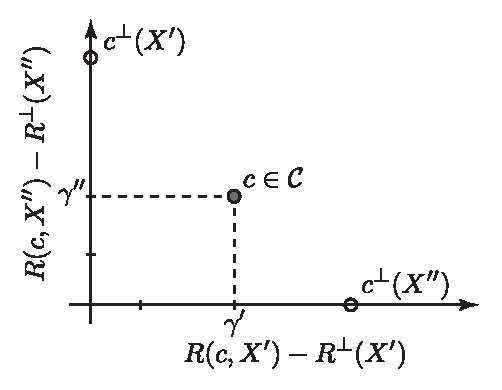
\includegraphics[width=\linewidth]{figures/ch_generic_approach/approx_sets--schematic--1}
      \caption{Placing a solution $c \in \C$}
  \end{subfigure}
  \\[.5cm]
  \begin{subfigure}[b]{.55\textwidth}
      \label{fig:approx_sets--example--3}
      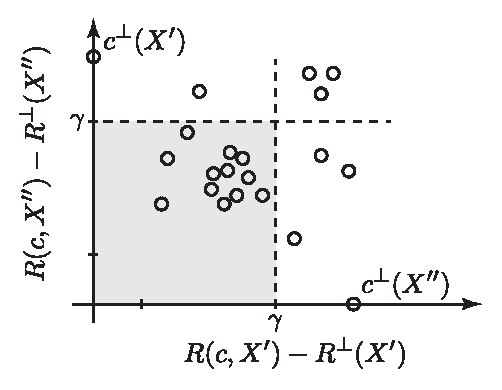
\includegraphics[width=\linewidth]{figures/ch_generic_approach/approx_sets--schematic--3}
      \caption{Intersection $\mathcal{C}_{\gamma}(X')\cap \mathcal{C}_{\gamma}(X'')$}
  \end{subfigure}
  \\[.5cm]
  \caption{
    Approximation sets for the instances $X'$ and $X''$. By $c^\bot(X)$ we
    denote the solution whose cost is minimum in $X$. \textbf{(a)}: We
    place each solution $c \in \mathcal{C}$ at position
    $(\gamma',\gamma'')$, where $\gamma'=R(c, X') - R^\bot(X')$ and
    $\gamma''=R(c, X'') - R^\bot(X'')$. \textbf{(b)}: Example of
    intersection of approximation sets $\mathcal{C}_{\gamma}(X')\cap
    \mathcal{C}_{\gamma}(X'')$ (this view on approximation sets was 
    originally suggested by Tobias Pröger~\citep[cf.][]{jcss:2017}, figure labels
    adapted for additive notation).}
  \label{fig:approx_sets--schematic}
\end{figure}
%
Thus we have 
\begin{equation}
  |{\mathcal{C}_\gamma}(X') \cap {\mathcal{C}_\gamma}(X'')|=sim(\gamma)+
    es(\gamma,k(\gamma),l(\gamma)),
\end{equation}
and, to maximize the probability that the uniformly randomly
chosen solution from the intersection is stable, we want to find the value $\gamma$ that maximizes
$\frac{sim(\gamma)}{sim(\gamma)+es(\gamma,k(\gamma),l(\gamma))}$. The following about 
maximization objectives holds:
\begin{align}
  \arg \max_{\gamma>0} &\;\; \frac{sim(\gamma)}{sim(\gamma)+es(\gamma,k(\gamma),l(\gamma))}  \notag \\
    &\qquad= \arg \max_{\gamma > 0} \; \Bigl(
        1 - \frac{es(\gamma,k(\gamma),l(\gamma))}{sim(\gamma)+es(\gamma,k(\gamma),l(\gamma))}
      \Bigr) \notag \\
    &\qquad= \arg \min_{\gamma > 0} \;\; \frac{es(\gamma,k(\gamma),l(\gamma))}{sim(\gamma)+es(\gamma,k(\gamma),l(\gamma))}
      \notag \\
    &\qquad= \arg \max_{\gamma > 0} \;\; \frac{sim(\gamma)+es(\gamma,k(\gamma),l(\gamma))}{es(\gamma,k(\gamma),l(\gamma))},
\end{align}
hence we can reformulate (for the sake of clarity) the objective of the similarity-based
approach as maximizing the value
\begin{align}
  \label{eq:similarity}
  S_\gamma(X',X'')
    \coloneqq \frac{|{\mathcal{C}_\gamma}(X') \cap {\mathcal{C}_\gamma}(X'')|}{es(\gamma,k(\gamma),l(\gamma))}
    = \frac{sim(\gamma)+es(\gamma,k(\gamma),l(\gamma))}{es(\gamma,k(\gamma),l(\gamma))}.
\end{align}


\begin{figure}[t!]
  \centering
  \begin{subfigure}[b]{.49\textwidth}
      \label{fig:intersection_due_to_gamma} 
      \includegraphics[width=\linewidth]{figures/ch_generic_approach/intersection_due_to_gamma}
      \caption{Two non-similar approximation sets.}
  \end{subfigure}
  \hfill
  \begin{subfigure}[b]{.49\textwidth}
      \label{fig:intersection_due_to_sim}
      \includegraphics[width=\linewidth]{figures/ch_generic_approach/intersection_due_to_sim}
      \caption{Two similar approximation sets}
  \end{subfigure}
  \\[.5cm]
  \caption{Illustration of ideas contained in Definitions~\ref{def:feasible_as},
  \ref{def:intersection_due_to_gamma} and \ref{def:intersection_due_to_sim}: as
  opposed to randomly chosen approximation sets \textbf{(a)}, two related
  (similar) approximation sets \textbf{(b)} have a $sim(\gamma)$ component of
  the intersection, which we naturally seek to maximize.}
  \label{fig:intersection_types}
\end{figure}

\paragraph{Problem-based instance similarity}
In equation~\eqref{eq:similarity}, the expected size of the intersection is
w.r.t.\  the problem specific probability distribution over all feasible
approximation sets of size $|{\mathcal{C}_\gamma}(X')|$ and
$|{\mathcal{C}_\gamma}(X'')|$, respectively. However, this distribution is hard
to estimate, so,~\citet{Sramek:PhD} introduced a problem-based based instance
similarity, which approximates the denominator by a uniformly chosen pair of
approximation sets.
\index{Similarity approach!Problem-based similarity}
%
\begin{definition}[Problem-based instance similarity]
  Let $X'$ and $X''$ be two input instances of a combinatorial optimization
  problem $\mathcal{P}$ with solution space $\mathcal{C}$. For a given $\gamma$,
  let ${\mathcal{C}_\gamma}(X')$ and ${\mathcal{C}_\gamma}(X'')$ be $\gamma$-approximation sets for $X'$
  and $X''$. Further, let $\mathcal{F}_k$ denote the set of all feasible
  approximation sets of size $k$, i.e., the set of all such sets $F\subseteq
  \mathcal{C}$ of size $k$ for which there exists an instance $I'$ and
  a value $\tilde \gamma$ such that $F=\mathcal{C}_{\tilde \gamma}(\tilde X)$. Then, the expression
  \begin{equation}
    \label{eq:generic_similarity}
    S_\gamma(X',X'') = \frac{|{\mathcal{C}_\gamma}(X')\cap {\mathcal{C}_\gamma}(X'')|}
      {\mathop{\mathbb{E}}_{A\in \mathcal{F}_{|{\mathcal{C}_\gamma}(X')|}, B\in
      \mathcal{F}_{|{\mathcal{C}_\gamma}(X'')|}}{\big[|A\cap B|\big]}}
  \end{equation}
  \nomenclature[D, 03c]{$S_\gamma(X',X'')$}{instance $\gamma$-similarity}%
  \nomenclature[D, 04]{$\mathcal{F}_k$}{all feasible approximation sets}%
  is the \emph{similarity of $X'$ and $X''$ at value $\gamma$} (with respect to
  the optimization problem $\mathcal{P}$), and the expression
  \begin{equation}
    \label{def:S}
    S(X',X'') \coloneqq \max_\gamma S_\gamma(X',X'')
  \end{equation}
  \nomenclature[D, 03d]{$S(X',X'')$}{instance similarity}%
  is the \emph{similarity of $X'$ and $X''$} with respect to the optimization
  problem $\mathcal{P}$.
\end{definition}
%

Thus, the similarity-based approach (in the following referred just as
``similarity'' approach) works as follows. First, we compute the value $\gamma$
that maximizes the similarity
\begin{align}\label{eq:similarity_formula}
  S_\gamma(X',X'') = \frac{|{\mathcal{C}_\gamma}(X')\cap {\mathcal{C}_\gamma}(X'')|}
    {\mathop{\mathbb{E}}_{A\in \mathcal{F}_{|{\mathcal{C}_\gamma}(X')|}, B\in
    \mathcal{F}_{|{\mathcal{C}_\gamma}(X'')|}}{\big[|A\cap B|\big]}},
  \tag{\ref{eq:generic_similarity}}
\end{align}
where the expectation is w.r.t.\ the uniform probability distribution over the
elements in $\mathcal{F}_{|{\mathcal{C}_\gamma}(X')|}$ and $\mathcal{F}_{|{\mathcal{C}_\gamma}(X'')|}$,
respectively. We then return a solution from ${\mathcal{C}_\gamma}(X')\cap {\mathcal{C}_\gamma}(X'')$
uniformly at random.

However, there are two practical issues with the procedure shown above: a)~it is
not always clear how to directly optimize $\gamma$ for the value
of~\eqref{eq:generic_similarity}; and b)~sampling from the intersection of the
corresponding $\gamma$-approximation sets uniformly at random might be
difficult. Despite all that, the similarity approach can be always applied in the 
cases, where one can provide all the steps of Algorithm~\ref{alg:similarity}.

\medskip
\begin{algorithm}[ht!]
\caption{Pipeline for Similarity Approach (Section~\ref{sec:similarity_approach_intro})}
\label{alg:similarity}
  {Determine the domains $\mathcal{F}_k$ of feasible approximation sets of size
  $k$.}

  {Provide a mathematical analysis or an algorithm $ALG_\mathbb{E}$ that
  computes the expected size of the intersection of two approximation sets of
  given sizes $k$ and $l$.}

  {Provide an algorithm $ALG_\cap$ that computes the size of the intersection
  ${\mathcal{C}_\gamma}(X')\cap {\mathcal{C}_\gamma}(X'')$, given $\gamma$ and
  two instances $X'$ and $X''$.}

  {Find $\gamma^*$ that maximizes the similarity $S_\gamma(X',X'')$, using
  $ALG_\mathbb{E}$ and $ALG_\cap$.}

  {Provide an algorithm $ALG_\text{rand}$ that picks a uniform random solution
  from the intersection $\C_{\gamma^*}(X')\cap \C_{\gamma^*}(X'')$.}
\end{algorithm}
\medskip

In order to fulfill these tasks, on can use several tools provided below. It is
important to notice that these useful theorems close the
gap between the ASC formulation~\eqref{eq:asc_mutual_information_formula} and the
similarity approach formulation~\eqref{eq:similarity_formula}.

\begin{theorem}[\citealp{Sramek:PhD}]
  \label{thm:simple}
  Let $\mathcal{P} = (\mathcal{X}, \mathcal{C}, R)$
  (see~Section~\ref{sec:optimization_problem_description}) be an optimization
  problem with the property that for any subset $F$ of the set of all feasible
  solutions $\mathcal{C}$ there exists an instance $\tilde X \in \mathcal{X}$
  and a value $\tilde \gamma$ such that $\mathcal{C}_{\tilde \gamma}(\tilde
  X)=F$. Then, the similarity of two instances $X', X''\in\mathcal{X}$ at value
  $\gamma$ is
  \begin{align}
    \label{eq:simple}
    S_\gamma(X',X'')=\frac{|\mathcal{C}||{\mathcal{C}_\gamma}(X') \cap {\mathcal{C}_\gamma}(X'')|}
      {|{\mathcal{C}_\gamma}(X')||{\mathcal{C}_\gamma}(X'')|}.
  \end{align}
\end{theorem}

However, as \citet{Sramek:PhD} notes, there exists an issue that not every subset
$F\subseteq\mathcal{C}$ is a feasible approximation set, and there is still no general
algorithm of computing the expected size of the intersection. The following
chain of theorems provides some approximation guarantees for the value of~\eqref{eq:simple}.

\begin{theorem}[\citealp{Sramek:PhD}]
  \label{thm:bound}
  Let $\mathcal{P} = (\mathcal{X}, \mathcal{C}, R)$ be an optimization problem. If
  $|{\mathcal{C}_\gamma}(X')|=|{\mathcal{C}_\gamma}(X'')|$ for a given $\gamma$, then
  \begin{align}
    \label{eq:bound}
    S_\gamma(X',X'') \leq \frac{|\mathcal{C}||{\mathcal{C}_\gamma}(X')\cap {\mathcal{C}_\gamma}(X'')|}
      {|{\mathcal{C}_\gamma}(X')||{\mathcal{C}_\gamma}(X'')|}.
  \end{align}
\end{theorem}

\begin{theorem} [\citealp{Sramek:PhD}]
  \label{thm:approx}
  Let $A$ be a constant such that for each feasible solution $c$ of some
  optimization problem $\mathcal{P} = (\mathcal{X}, \mathcal{C}, R)$ it holds that 
  $|\{F\in \mathcal{F}_k | c\in F\}| \leq A k|\mathcal{F}_k|/|\mathcal{C}|$. Then,
  \begin{align}
    S_\gamma(X',X'')\geq\frac{|\mathcal{C}||{\mathcal{C}_\gamma}(X')\cap {\mathcal{C}_\gamma}(X'')|}
      {A |{\mathcal{C}_\gamma}(X')||{\mathcal{C}_\gamma}(X'')|}.
  \end{align}
\end{theorem}

\begin{theorem} [\citealp{Sramek:PhD}]
  \label{thm:worst_case}
  Let $\mathcal{P} = (\mathcal{X}, \mathcal{C}, R)$ be an optimization problem.
  Then,
  \begin{align}
    S_\gamma(X',X'')\geq\frac{|{\mathcal{C}_\gamma}(X')\cap {\mathcal{C}_\gamma}(X'')|}{|{\mathcal{C}_\gamma}(X')||{\mathcal{C}_\gamma}(X'')|}.
  \end{align}
\end{theorem}
%

\myremark This shows that the step of deriving the appropriate specific formula or
algorithm to calculate the expected size of the intersection is a necessary
component of the approach, unless it is possible to show that for a concrete
problem the upper bound is sufficient. We will speculate more on that in the
conclusion to this chapter (Section~\ref{sec:gen_appch_conclusion}).

\section{Proof-of-Concept Prototypic Example}
\label{sec:proof_of_concept}

\index{Prototypic example!For ASC}
Previously, in Section~\ref{sec:asc_original}, we introduced a method of
solution regularization by ASC, and later in
Section~\ref{sec:similarity_approach_intro} we gave a thorough overview of an
analogical approach called instance similarity. While they stem from completely
different roots, it can be easily seen that they both aim at choosing an optimal
approximation set width $\gamma$ in a same way. Specifically, we seek to
optimize
\begin{equation}\label{eq:similarity_maximization_objective}
    \gamma^* = \arg \max_{\gamma >0} \frac{|{\mathcal{C}_\gamma}(X') \cap {\mathcal{C}_\gamma}(X'')|}
      {|{\mathcal{C}_\gamma}(X')||{\mathcal{C}_\gamma}(X'')|}
\end{equation}
\myremark Note that this equation is
\textit{not} identical either to its ASC
version~\eqref{eq:asc_mutual_information_formula} or similarity-based
version~\eqref{eq:similarity_formula}, although yielding same optimization goal;
we will briefly revisit the technical differences, like presence of logarithm,
later in the conclusion.

One of the contributions of this thesis is to present an abstract
proof-of-concept model for prototypical combinatorial optimization problems,
which would allow to experimentally the advantages of the approximation set-based 
approaches. We will mostly experimentally investigate how the methods of
Sections~\ref{sec:asc_original} and~\ref{sec:similarity_approach_intro} perform
on this model.

\subsection{The Example Setting and Terminology}
We expect the approximation set-based methods to exceed the performance of other
optimization methods when the set of solutions that have stable cost over all or
most instances is large enough not to be completely hidden in the noise.
%
To highlight the potential of our approach, we consider an uncertain
minimization problem $(\mathcal{X}, \mathcal{C}, R)$ in which the solution space
$\mathcal{C}$ is partitioned into two sets $\sgood$ and $\sbad$ of sizes $\g$
and $\b$, respectively, which contain the \good\ and the \bad\ solutions,
respectively. Without loss of generality we assume that
\begin{align}
  \C &= \{c_i\}_{i=1}^n \notag \\
  \sgood &= \{c_1,\ldots, c_{|\g|}\} \notag \\
  \sbad &= \{c_{|\g|+1},\ldots,c_{|\g|+|\b|}\}.
\end{align}
\nomenclature[D, 04a]{$\sgood$, $\sbad$}{\good\ and \bad\ solutions}%
%
The sets $\sgood$ and $\sbad$ represent solutions which are desirable and
non-desirable to be chosen, which reflects the fact that the approximation
set-based approaches are designed to reliably tell them apart. We further assume
that $\g \ll \b$, which corresponds to the fact that \good\ solutions should be hard
to identify.

Our proof-of-concept scenario abstracts from a concrete optimization problem. In
other words, we do not address here the problem of specific optimization
algorithms. Hence we explicitly state that instead of generating inputs $X \in
\mathcal{X}$, we rather directly generate costs of solutions $c \in \C$.
%
In the terminology of Section~\ref{sec:optimization_problem_description}, an
instance $X$ can be represented as a vector of random solution costs of length
$n$:
\begin{equation}\label{eq:generic_appch_cost_vector}
  X \coloneqq \langle R_i \rangle_{i=1}^{n},
\end{equation} 
and the cost function is simply
\begin{equation}
  R(c_i, X) \coloneqq R_i,
\end{equation} 
i.e.~the $i$-th entry stores the cost of the solution $c_i$ in $X$.

\subsection{Problem Generation}
\label{sec:gen_appch_pg}

We define the solution ``desirability'' by the intuition that costs of \good\
solutions have a small standard deviation and play the role of signal,
while costs of \bad\ solutions have a higher mean and/or a higher standard
deviation and play the role of deceiving noise.

We assume the cost vector of an instance $X$ to be generated with the following
random problem generating process $PG(\cdot)$:
\begin{itemize}
  \item[1)] the first $\g$ values are chosen at random according to some
            (fixed) probability distribution $\DG$, and
  \item[2)] the remaining $\b$ values are chosen at random according to some
            (fixed) probability distribution $\DB$.
\end{itemize}
\nomenclature[D, 04b]{$\DG$, $\DB$}{cost distributions\nomnorefeq}%

\begin{figure}[t!]
  \centering
  \begin{subfigure}[b]{.8\textwidth}
      \includegraphics[width=\linewidth]{figures/ch_generic_approach/stable_and_unstable_distr}
  \end{subfigure}
  \caption{Schematic example of \good\ and \bad\ cost distributions and noise
  levels $N \in \mathcal{N}$ of \bad\ ones, as described in
  Section~\ref{sec:gen_appch_pg}.}
  \label{fig:stable_and_unstable_solutions}
\end{figure}

Naturally it is safe to assume that both $\DG$ and $\DB$ have the property that
\good\ solutions are superior to \bad\ ones
(Figure~\ref{fig:stable_and_unstable_solutions}), e.g., because they have a
smaller expected cost or a smaller variance, i.e. for any $R_\text{\good} \sim
\DG$ and $\R_\text{\bad} \sim \DB$, $\Expct [R_\text{\good}] < \Expct [R_\text{\bad}]$ 
and $\Var [R_\text{\good}] < \Var [R_\text{\bad}]$.
We further assume $\DG$ and $\DB$ are independent of the
instance and of the concrete solution (costs of \good\ solutions are always
chosen from $\DG$, costs of \bad\ solutions are always chosen from $\DB$).

We model noise in a generic way by defining a set of noise levels $\mathcal{N}$
(the concrete definition depends on the type of the noise, see~\citep{jcss:2017}). For a fixed noise
level $N\in\mathcal{N}$, we randomly generate an instance as follows. \Good\
solutions are drawn from a distribution with fixed mean $\mu_\mathrm{\G}$ and fixed
standard deviation $\sigma_\mathrm{\G}$.
\Bad\ solutions are drawn from a distribution with mean $\mu_\mathrm{\B}(N)$ and standard
deviation $\sigma_\mathrm{\B}(N)$. The distributions of the \bad\ solutions are
chosen in a way such that for every two noise levels $N,N'\in\mathcal{N}$ with
$N'>N$, we have $\mu_\mathrm{\B}(N')<\mu_\mathrm{\B}(N)$ or
$\sigma_\mathrm{\B}(N')>\sigma_\mathrm{\B}(N)$.
\nomenclature[D, 04c]{$N \in \mathcal{N}$}{noise levels for experiment\nomnorefeq}%

\myremark Such assumptions on noise levels are justified by the fact that noise
would naturally imply either a smaller expected cost, or a higher standard
deviation, or both~--- resulting in a more aggressive ``deceiving'' of the
algorithm. See Figure~\ref{fig:stable_and_unstable_solutions} for schematic
illustration of this intuition.

Due to its enormous theoretical and practical relevance, we present here the
results for the Gaussian noise model (for more noise settings, see~\citep{jcss:2017}).
 \Good\ solutions are drawn from a Gaussian
distribution with mean $\mu_{\G}=1$ and standard deviation $\sigma_{\G}=1$. We
define the noise levels $\mathcal{N}$ in such a way that for each noise level
$N\in\mathcal{N}$, \bad\ solutions are drawn from a Gaussian distribution with
mean $\mu_{\B}(N)=10$ and standard deviation $\sigma_{\B}(N)=N$: $\DG = \mathrm{Norm}(1, 1)$ and
$\DB(N) = \mathrm{Norm}(10, N^2)$.

\subsection{The Goal and Success Metrics}

Now, our goal is the following: given two instances $X'$ and $X''$ generated by
the random process $PG(\cdot)$ described above, our algorithm $\mathscr{A}$ has
to compute a set of solutions $\hat \C_\mathscr{A}$ of candidates for solutions in
$\sgood$, from which it then picks a solution
uniformly at random. The only knowledge of an
algorithm consists of the two cost vectors of $X'$ and $X''$ defined
in~\eqref{eq:generic_appch_cost_vector}. The algorithm cannot exploit the fact
that there are two categories of solutions, and in particular it has no
knowledge about $\DG$ and $\DB$.

Since we assume that a solution from $\hat{\mathcal{C}}_{\mathscr{A}}$ is
picked uniformly at random, we define the \emph{success probability} of $\mathscr{A}$
with input $X'$ and $X''$ as
\begin{align}
  \label{eq:uncert:prob_succ}
  P_{\mathscr{A}}(X',X'')
    = \frac{|{\mathcal{C}}_\mathscr{A}\cap\sgood|}{|{\mathcal{C}}_\mathscr{A}|}
      \text{, for a solving algorithm } \mathscr{A}.
\end{align}
\nomenclature[D, 04d]{$P_{\mathscr{A}}(X',X'')$}{success metric for experiment}%

We want to investigate how the success probabilities of the similarity algorithm
proposed in this chapter evolves with increasing noise, and benchmark it against
some other algorithms. In this thesis, we present only a Joint Minimizer algorithms
(see next section), but for the results produced on a more complete list of benchmarks
we refer the reader to~\citep{jcss:2017}.

\subsection{Experimental Results}
\label{sec:continuous_noise}

\paragraph{Benchmark: joint cost minimizing}
When only two instances are given, the most efficient and straightforward idea
to find a solution that is likely to be good for a test instance is to compute
a solution~$c$ that minimizes the average cost, or equivalently, the joint cost
$R(c, X')+R(c, X'')$. We refer to this method as the \textit{Joint Minimizer}
method in the plots below.
\index{Joint cost minimizer}
\index{Joint minimizer|see{Joint cost minimizer}}

\paragraph{Results}

For each noise level $N\in\mathcal{N}$, we perform the following
experiment: we generate $\R=1000$ instance pairs $(X',X'')_{k\in\{1,\ldots,
\R\}}$ with noise level $N$ according to the $PG(\cdot)$ process described in
Section~\ref{sec:gen_appch_pg}, and for each of these instance pairs we compute
$P_\mathscr{A}(X',X'')$ for all algorithms $\mathscr{A}$. After that we set
\begin{align}
  \hat P_\mathscr{A}(N) &\coloneqq \frac{1}{\R} \sum_{k=1}^{\R} P_\mathscr{A}(X',X'')
\end{align}
to estimate the average success probability of the proposed methods in
dependency of the noise level $N$. Unless otherwise stated, $\mathcal{C}$
contains $n=1000$ solutions.

In our experiments, $\R=1000$ repetitions turned out to be enough to exhibit
the behaviors of the methods. Preliminary experiments with $10000$ repetitions
gave similar results: the rankings of the methods were the same, only the curves in
the plots appeared to be smoother.

Figure~\ref{fig:gnm} shows that the experimental results for
Gaussian noise show a strong indication that the approximation set-based similarity
approach is very competitive against the joint cost minimization.
\begin{figure}[t!]
  \centering
  \begin{subfigure}[b]{.49\textwidth}
      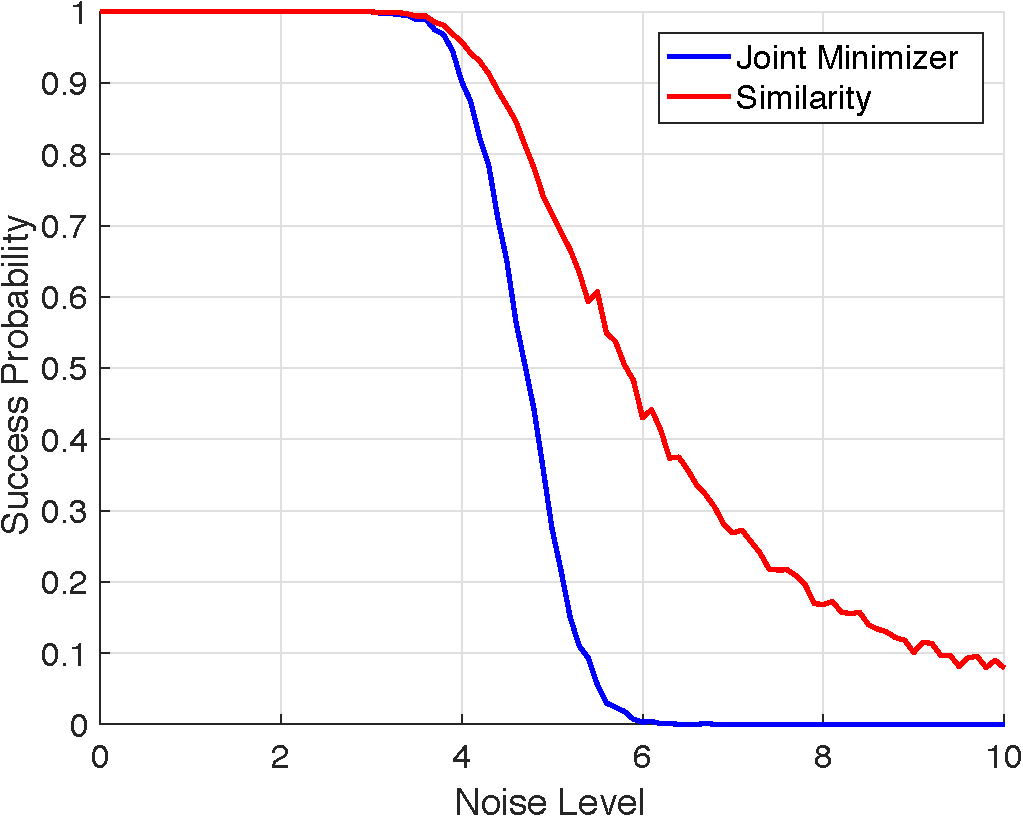
\includegraphics[width=\linewidth]{figures/ch_generic_approach/gnm_g50_b950}
      \caption{$5\%$ of solutions are \good.}
      \label{fig:gnm_5}
  \end{subfigure}
  \hfill
  \begin{subfigure}[b]{.49\textwidth}
      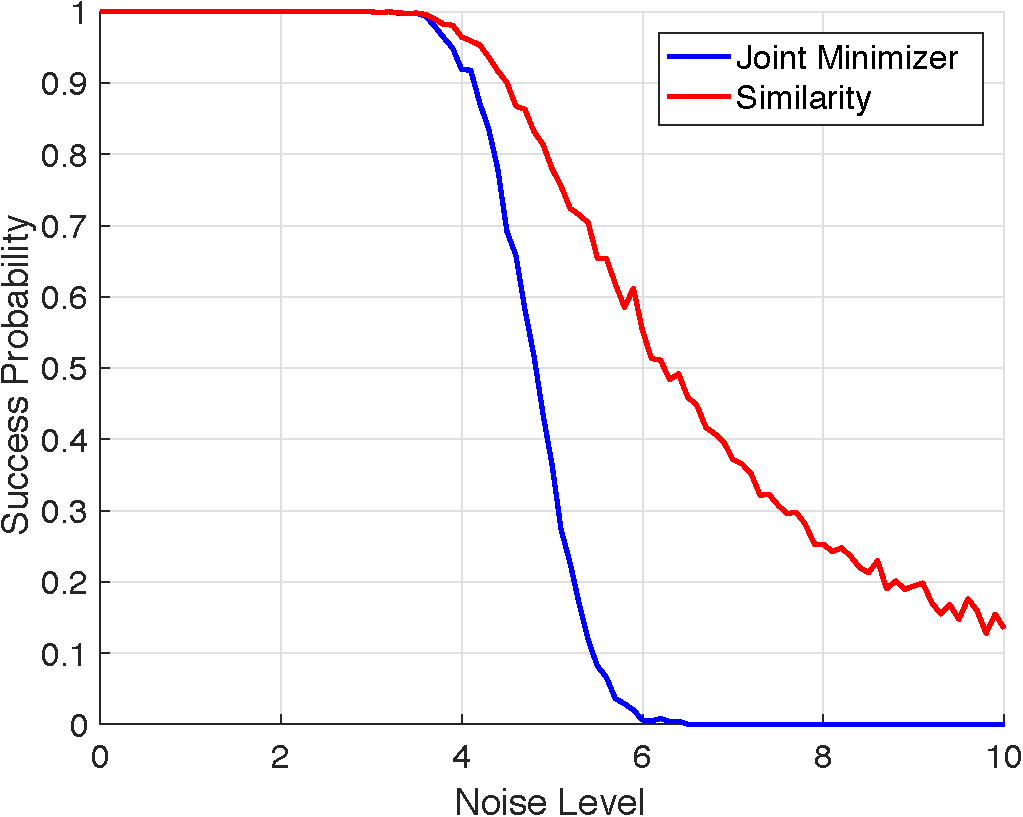
\includegraphics[width=\linewidth]{figures/ch_generic_approach/gnm_g100_b900}
      \caption{$10\%$ of solutions are \good.}
      \label{fig:gnm_10}
  \end{subfigure}
  \\[.5cm]
  \begin{subfigure}[b]{.49\textwidth}
      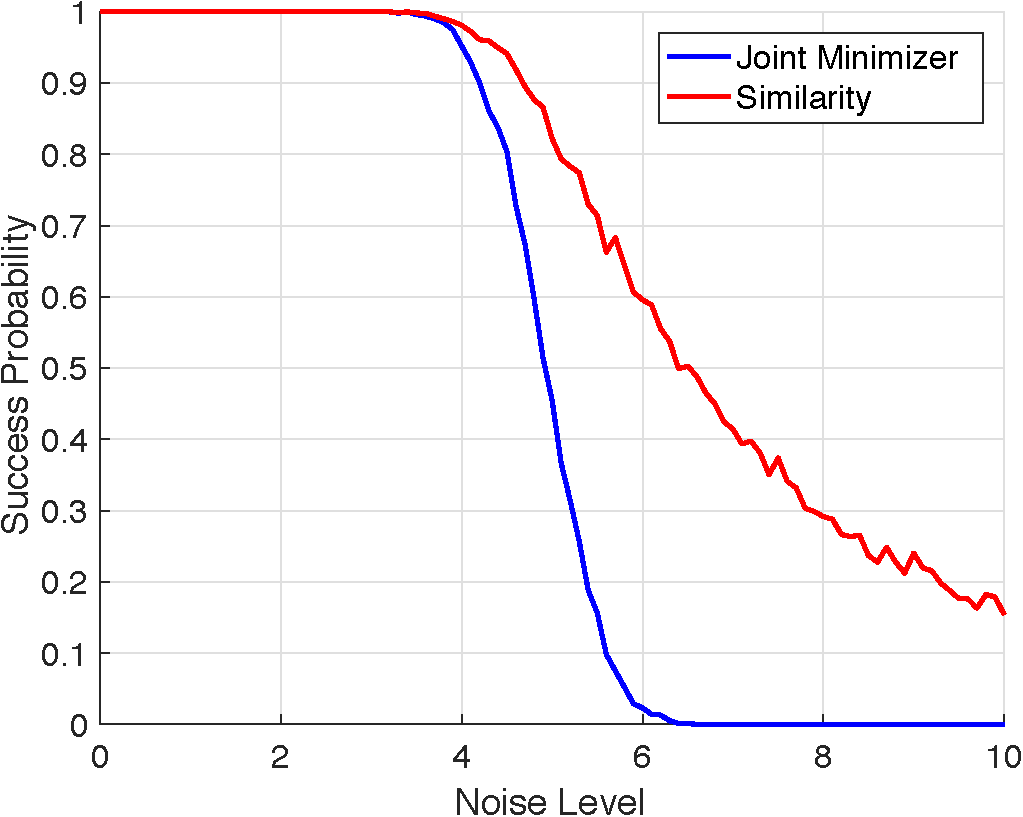
\includegraphics[width=\linewidth]{figures/ch_generic_approach/gnm_g200_b800}
      \caption{$20\%$ of solutions are \good.}
      \label{fig:gnm_20}
  \end{subfigure}
  \hfill
  \begin{subfigure}[b]{.49\textwidth}
      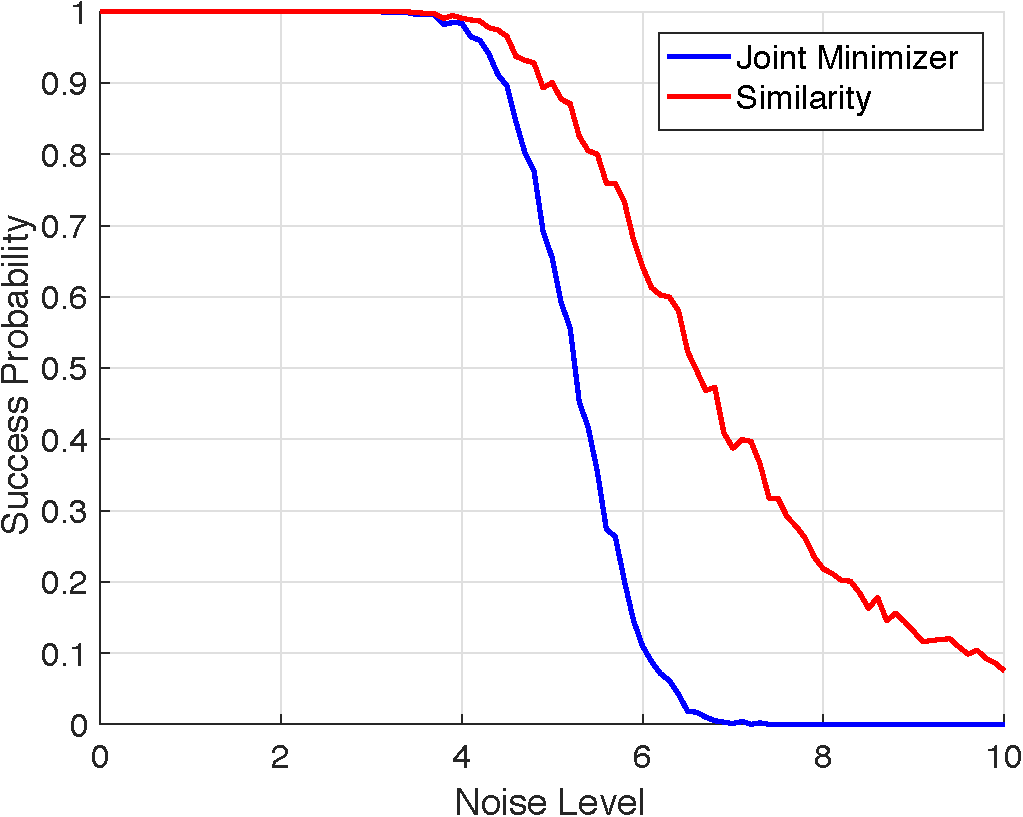
\includegraphics[width=\linewidth]{figures/ch_generic_approach/gnm_g500_b500}
      \caption{$50\%$ of solutions are \good.}
      \label{fig:gnm_50}
  \end{subfigure}
  \\[.5cm]
  \caption{Experimental results where $5\%$ \textbf{(a)}, $10\%$ \textbf{(b)},
    $20\%$ \textbf{(c)} and $50\%$ \textbf{(d)} of the solutions are \good.
    Total number of solutions equals $1000$.}
  \label{fig:gnm}
\end{figure}
Note that the latter is a straightforward way to compute solutions, when only two
inputs are provided. 

\section{Finding Optimal Approximations Analytically}
\label{sec:analytic_solution}

\subsection{Theoretical Results}

One of our main assumptions was that the noise generating process is unknown to
the predicting algorithm $\mathscr{A}$. It was also previously noted that the
crucial step of the whole approximation set-based approach consists in deriving
the appropriate specific formula or algorithm to calculate the
similarity~\eqref{eq:simple}. As a first step towards a formal analysis of the
model discussed in the previous section, in this section we thoroughly
investigate how the similarity~\eqref{eq:simple} behaves in expectation (where
the expectation is computed over all pairs of instances generated by the random
process $PG(\cdot)$), i.e., we analyze the function
\begin{equation}
  \label{eq:oracle_similarity}
  S_\gamma^{\mathrm{EXP}}=\mathbb{E}_{X',X''\sim PG} \,
    S_\gamma(X',X'').
\end{equation}
\index{Similarity approach!Calibration assumption}
\index{Calibration assumption|see{Similarity approach}}
For simplicity we introduce the \emph{calibrating assumption} that the minimum
solutions of both instances $X'$ and $X''$ have the same cost $m$:
\begin{equation}\label{eq:gen_appch_calibrating_assumption}
  \min_c R(c, X') \approx \min_c R(c, X'') \approx m.
\end{equation} 
Without this assumption our analysis would still be possible, but it would be
more technical. Notice that the assumption does not imply that the minimum
solutions themselves are the same: in general, it holds that
\begin{equation}
   \arg \min_c R(c, X') \ne \arg \min_c R(c, X''),
\end{equation} 
i.e. minimum costs are not necessarily attained on the same solution.

\index{Similarity approach!Theoretical estimator}
\begin{theorem}
\label{thm:oracle_similarity}
Let $\gamma>0$, $V = |\mathcal{C}_\gamma(X')\cap \mathcal{C}_\gamma(X'')|$,
$W = |\mathcal{C}_\gamma(X')|\cdot |\mathcal{C}_\gamma(X'')|$, $m$ be the minimum cost of a
solution in both $X'$ and $X''$ (i.e., the calibrating assumption is
satisfied), and $\FG$ and $\FB$ denote the cumulative density functions of the
\good\ and the \bad\ solutions, respectively, evaluated at $m+\gamma$. Then, the
expected similarity~\eqref{eq:oracle_similarity} can be approximated by the
estimated similarity
\begin{align}
  \label{eq:esim}
  S_\gamma^{\mathrm{EXP}} \sim \hat S_\gamma \coloneqq |\mathcal{C}|\left(
    \frac{\Expct[V]}{\Expct[W]} -
    \frac{\Cov(V,W)}{\Expct[W]^2} + \frac{\Var[W] \cdot \Expct[V]}{\Expct[W]^3}\right)
\end{align}
\nomenclature[D, 05]{$S_\gamma^{\mathrm{EXP}}$, $\hat S_\gamma$}{theoretical estimator of similarity}%
where
\begin{align}
  \label{eq:esim:ev}
  \Expct[V] &= \g\FG^2 + \b\FB^2, \\
  \label{eq:esim:ew}
  \Expct[W] &= (\g\FG + \b\FB)^2, \\
  \label{eq:esim:cov}
  \Cov(V, W) &= \g\FG^2(1 - \FG^2) + 2\g(\g-1) \FG^3(1 - \FG) \notag \\
    &\quad + 2\g\b\FG^2\FB (1 - \FG) + 2\g\b\FG\FB^2(1 - \FB) \notag \\
    &\quad + \b\FB^2(1 - \FB^2) + 2\b(\b-1) \FB^3(1 - \FB), \text{ and} \\
  \label{eq:esim:var}
  \Var[W] &= \g^2\FG^2(1- \FG^2) + 2\g^2(\g-1)\FG^3(1 - \FG) \notag\\
    &\quad + 2\g\b(\b - 1) \FG \FB^2 (1 - \FG) \notag\\
    &\quad + 2\g(\g - 1)\b \FG^2 \FB (1 - \FB) \notag\\
    &\quad + 2\g\b \FG \FB (1 - \FG\FB) \notag\\
    &\quad + \b^2 \FB^2 (1 - \FB^2) + 2\b^2(\b-1) \FB^3 (1 - \FB) \notag\\
    &\quad + 4 \g^2 \b \FG^2 \FB (1 - \FG) + 4\g\b^2 \FG \FB^2 (1 - \FB).
\end{align}
\end{theorem}

\paragraph{Proof of Theorem~\ref{thm:oracle_similarity}}
To make this proof more readable, we break it down into several
steps.
\begin{itemize}
  \item[1)] {\em Preliminaries.}
    Let $m=\min_{c \in \mathcal{C}} R(c, X')=\min_{c \in \mathcal{C}} R(c, X'')$. Let
    $c_i$, $i\in\{1,\ldots,\g\}$ denote the solutions in $\sgood$ and
    $\bar c_i$, $i\in\{1,\ldots,\b\}$ denote the solutions in $\sbad$. We define
    \begin{align*}
      A'_{i, \gamma} &= \mathbbm{1}\{R(c_i,X') \le m+\gamma\}, \quad 1 \le i \le \g \\
      A''_{i, \gamma} &= \mathbbm{1}\{R(c_i,X'') \le m+\gamma\}, \quad 1 \le i \le \g \\
      B'_{j, \gamma} &= \mathbbm{1}\{R(\bar c_j,X') \le m+\gamma\}, \quad 1 \le j \le \b \\
      B''_{j, \gamma} &= \mathbbm{1}\{R(\bar c_j,X'') \le m+\gamma\}, \quad 1 \le j \le \b.
    \end{align*}
    \nomenclature[A, 00]{$\mathbbm{1}\{\cdot\}$}{indicator function\nomnorefeqpage}%
    Now the components of the similarity~\eqref{eq:similarity} can be
    expressed as
    \begin{align*}
      |\mathcal{C}_\gamma(X')\cap \mathcal{C}_\gamma(X'')|
        &= \sum_{i = 1}^{\g} A'_{i,\gamma} A''_{i,\gamma} +
          \sum_{j = 1}^{\b} B'_{j,\gamma} B''_{j,\gamma}, \\
      |\mathcal{C}_\gamma(X')|
        &= \sum_{i = 1}^{\g} A'_{i,\gamma} + \sum_{j = 1}^{\b} B'_{j,\gamma}, \\
      |\mathcal{C}_\gamma(X'')|
        &= \sum_{i = 1}^{\g} A''_{i,\gamma} + \sum_{j = 1}^{\b} B''_{j,\gamma}.
    \end{align*}
    For the rest of this proof we will simplify the notation as follows:
    1)~$\gamma$~is omitted in the subscript because we can assume it to be
    the same throughout all considerations, 2) the limits in the sums are
    omitted; for \good\ solutions we
    always sum up to $\g$ and for \bad\ solutions to $\b$, and 3) by $\FG$ and
    $\FB$ we denote the cumulative density functions of \good\ and \bad\
    distributions, respectively, evaluated at $m+\gamma$:
    \begin{equation}
      \FG \coloneqq \FG(m + \gamma), \qquad \FB \coloneqq \FB(m + \gamma).
    \end{equation}
    Observe that 1) $\Expct[A'_i]=\Expct[A''_i]=\FG$ and $\Expct[B'_j]=\Expct[B''_j]
    =\FB$, 2) the random variables in $\{A'_i\}_i \cup \{A''_j\}_j \cup \{B'_k\}_k
    \cup \{B''_\ell\}_\ell$ are jointly independent, and 3) $(A'_i)^2=A'_i$,
    $(A''_i)^2=A''_i$, $(B'_j)^2=Y_j$ and $(B''_j)^2=Y_j$ because these are
    indicators. Also, remember that for jointly independent indicator random
    variables $Z_1, Z_2, Z_3$ with $\Expct[Z_i] = z_i$ we have
    \nomenclature[B, 00]{$\Expct[\cdot]$}{expected value\nomnorefeqpage}%
    \nomenclature[B, 00]{$\Var[\cdot]$}{variance\nomnorefeqpage}%
    \begin{align}
      \Cov(Z_1, Z_2)
        &= z_1 z_2 (1 - z_1 z_2) \label{eq:ag:covariance_general_2} \\
      \Cov(Z_1 Z_2, Z_1 Z_3 )
        &= z_1 z_2 z_3 (1 - z_1) \label{eq:ag:covariance_general_1}
    \end{align}
  \item[2)] {\em Taylor expansion of the expected similarity.}
    A second-order Taylor approximation of $\Expct[V/W]$ gives
    \begin{align}
      \tag{\ref{eq:esim}}
      \Expct\biggl[\frac{V}{W}\biggl]
        \approx \frac{\Expct[V]}{\Expct[W]} -
        \frac{\Cov(V,W)}{\Expct[W]^2} +
        \frac{\Var[W] \cdot \Expct[V]}{\Expct[W]^3}.
    \end{align}
    Remember that $V$ denotes the size of the intersection while $W$ is the
    product of the approximation set sizes. In the following, we will
    analyze each term of~\eqref{eq:esim} separately.
  \item[3)] {\em Expected values of $V$ and $W$.}
    \begin{align*}
      \tag{\ref{eq:esim:ev}}
      \Expct[V] = \sum_i \Expct[A'_i] \cdot \Expct[A''_i] +
        \sum_j \Expct[B'_j] \cdot \Expct[B''_j] = \g\FG^2 + \b\FB^2.
    \end{align*}
    Taking the independence of the random variables into account, for
    $\Expct[W]$ we obtain
    \begin{align*}
      \tag{\ref{eq:esim:ew}}
      \Expct[W]
        = \Expct\Bigl[\sum_i A'_i + \sum_j B'_j\Bigr] \cdot
          \Expct\Bigl[\sum_i A''_i + \sum_j B''_j\Bigr]
        = ( \g \FG + \b \FB )^2.
    \end{align*}
  \item[4)] {\em Analyzing the covariance of $V$ and $W$.}
    Remember that
    \begin{align}
      V &= \sum_i A'_i A''_i + \sum_i B'_i B''_i, \\
      W &= \sum_{j,k} A'_j A''_k + \sum_{i,j} A'_j B''_k +
        \sum_{j,k} B'_j A''_k + \sum_{j,k} B'_j B''_k,
        \label{eq:ag:w_representation}
    \end{align}
    hence
    \begin{align}
      \Cov(V, W)
        &= \sum_{i,j,k} \Cov( A'_i A''_i, A'_j A''_k ) + \sum_{i,j,k} \Cov( A'_i A''_i, A'_j B''_k ) \notag \\
        &+ \sum_{i,j,k} \Cov( A'_i A''_i, B'_j A''_k ) + \sum_{i,j,k} \Cov( A'_i A''_i, B'_j B''_k ) \notag \\
        &+ \sum_{i,j,k} \Cov( B'_i B''_i, A'_j A''_k ) + \sum_{i,j,k} \Cov( B'_i B''_i, A'_j B''_k ) \notag \\
        &+ \sum_{i,j,k} \Cov( B'_i B''_i, B'_j A''_k ) + \sum_{i,j,k} \Cov( B'_i B''_i, B'_j B''_k )
    \end{align}
    We will now analyze each of the single terms.
    \begin{itemize}
      \item[$\bullet$]
        In the first term $\sum \Cov( A'_i A''_i, A'_j A''_k )$
        only the summands with $j=i$ or $k=i$ are non-zero, hence we
        obtain
        \begin{align}
          \sum_{i,j,k} &\Cov( A'_i A''_i, A'_j A''_k )
             = \sum_i \Cov( A'_i A''_i, A'_i A''_i) \notag \\
            &\hspace{1cm}+ \sum_{i \ne j} \Bigl[ \Cov( A'_i A''_i, A'_i A''_j)
            + \Cov( A'_i A''_i, A'_j A''_i)\Bigr] \notag \\
            &= \sum_i \Cov( A'_i A''_i, A'_i A''_i)
            + 2 \sum_{i \ne j} \Cov( A'_i A''_i, A'_i A''_j), \notag\\
            &= \g \FG^2(1 - \FG^2)+2\g(\g-1) \FG^3 (1 - \FG),
            \label{eq:ag:comp_covariance_4}
        \end{align}
        where the last equality holds due
        to~\eqref{eq:ag:covariance_general_2}
        and~\eqref{eq:ag:covariance_general_1}.
      \item[$\bullet$]
        The next two terms $\sum \Cov( A'_i A''_i, A'_j B''_k )$ and
        $\sum \Cov( A'_i A''_i, B'_j A''_k )$ are equal to each other
        (due to the symmetry of $A'$ and $A''$), so their sum resolves
        to
        \begin{equation}
          2 \sum_{i,k} \Cov( A'_i A''_i, A'_i B''_k )
            \stackrel{\text{\eqref{eq:ag:covariance_general_1}}}{=}
            2 \g \b \FG^2 \FB ( 1 - \FG). \label{eq:ag:comp_covariance_2}
        \end{equation}
      \item[$\bullet$]
        The next two terms $\sum \Cov( A'_i A''_i, B'_j B''_k )$
        and $\sum \Cov( B'_i B''_i, A'_j A''_k )$ are both zero
        due to the independence of $A'_i A''_i$ and $B'_j B''_k$.
      \item[$\bullet$]
        The next two terms $\sum \Cov( B'_i B''_i, A'_j B''_k )$
        and $\sum \Cov( B'_i B''_i, B'_j A''_k )$ can be computed in
        exactly the same way as~\eqref{eq:ag:comp_covariance_2} where
        both $\FG$ and $\FB$ as well as $\g$ and $\b$ are interchanged.
        Hence, their sum equals
        \begin{equation*}
          2 \sum_{i,k} \Cov( B'_i B''_i, B'_i A''_k )
            \stackrel{\text{\eqref{eq:ag:covariance_general_1}}}{=}
            2 \g\b \FG \FB^2 ( 1 - \FB).
        \end{equation*}
      \item[$\bullet$]
        The last term $\sum \Cov( B'_i B''_i, B'_j B''_k )$ is computed
        similar as~\eqref{eq:ag:comp_covariance_4},
        performing the above-mentioned replacements, hence
        \begin{align*}
          \sum_{i,j,k} &\Cov( B'_i B''_i, B'_j B''_k )
            = \b \FB^2(1 - \FB^2) + 2\b(\b-1) \FB^3 (1 - \FB).
        \end{align*}
    \end{itemize}
  \item[5)] {\em Analyzing the variance of $W$.}
    Finally we compute $\Var[W] = \Cov(W, W)$. When $W$ is expressed
    as~\eqref{eq:ag:w_representation}, we obtain
    \begin{align*}
      \Cov(W, W)
      &= \sum_{i,j,k,\ell} \Cov(A'_i A''_j, A'_k A''_\ell) + \sum_{i,j,k,\ell} \Cov(A'_i B''_j, A'_k B''_\ell) \\
      &+\sum_{i,j,k,\ell} \Cov(B'_i A''_j, B'_k A''_\ell) + \sum_{i,j,k,\ell} \Cov(B'_i B''_j, B'_k B''_\ell) \\
      &+ 2 \sum_{i,j,k,\ell} \Cov(A'_i A''_j, A'_k B''_\ell) + 2 \sum_{i,j,k,\ell} \Cov(A'_i A''_j, B'_k A''_\ell) \\
      &+ 2 \sum_{i, j, k, \ell} \Cov(A'_i A''_j, B'_k B''_\ell) + 2 \sum_{i,j,k,\ell} \Cov(A'_i B''_j, B'_k A''_\ell) \\
      &+ 2 \sum_{i,j,k,\ell} \Cov(A'_i B''_j, B'_k B''_\ell) + 2 \sum_{i,j,k,\ell} \Cov( B'_i A''_j, B'_k B''_\ell).
    \end{align*}
    As before we analyze each of these terms separately.
    \begin{itemize}
      \item[$\bullet$]
        The first term $\sum \Cov(A'_i A''_j, A'_k A''_\ell)$ can be
        expressed as
        \begin{align*}
          &\sum_{i} \Cov(A'_i A''_i, A'_i A''_i)
            + 4 \sum_{i\ne j} \Cov(A'_i A''_i, A'_i A''_j) \\
          &+ 2\hspace{-4mm}\sum_{i \ne j, i \ne k, j \ne k}\hspace{-4mm} \Cov( A'_i A''_j, A'_i A''_k)
            + \sum_{i \ne j} \Cov( A'_i A''_j, A'_i A''_j)
        \end{align*}
        where
        \begin{align*}
          \sum_{i} \Cov(A'_i A''_i, A'_i A''_i) &= \g\FG^2(1 - \FG^2), \\
          4 \sum_{i\ne j} \Cov(A'_i A''_i, A'_i A''_j) &= 4\g(\g-1)\FG^3(1-\FG), \\
          2\hspace{-4mm}\sum_{i \ne j, i \ne k, j \ne k}\hspace{-4mm}
              \Cov( A'_i A''_j, A'_i A''_k) &= 2\g(\g-1)(\g-2) \FG^3( 1- \FG), \\
          \sum_{i \ne j} \Cov( A'_i A''_j, A'_i A''_j) &= \g(\g-1)\FG^2 ( 1 - \FG^2),
        \end{align*}
        and therefore
        \begin{equation}
          \label{eq:ag:comp_covariance_6}
          \sum_{i,j,k,\ell}\hspace{-1mm} \Cov(A'_i A''_j, A'_k A''_\ell)
            = \g \FG^2( 1- \FG^2) + 2 \g^2 (\g-1) \FG^3 ( 1- \FG).
        \end{equation}
      \item[$\bullet$]
        The next two terms $\sum \Cov(A'_i B''_j, A'_k B''_\ell)$ and
        $\sum \Cov(B'_i A''_j, B'_k A''_\ell)$ are equal due to the
        symmetry in instances, hence their sum equals
        \begin{align*}
          %&2 \sum_{i, j, k, \ell} \Cov(A'_i B''_j, A'_k B''_\ell) \\
          &2 \sum_{\substack{i \\ j \ne k}} \Cov(A'_i B''_j, A'_i B''_k)
            + 2 \sum_{\substack{i \\ j \ne k}} \Cov(A'_j B''_i, A'_k B''_i) \\
          &\quad + 2 \sum_{i, j} \Cov(A'_i B''_j, A'_i B''_j),
        \end{align*}
        where the the terms are computed as
        \begin{align*}
          2 \sum_{\substack{i \\ j \ne k}} \Cov(A'_i B''_j, A'_i B''_k)
            &\stackrel{\text{\eqref{eq:ag:covariance_general_1}}}{=}
              2 \g\b(\b-1) \FG \FB^2 (1 - \FG), \\
          2 \sum_{\substack{i \\ j \ne k}} \Cov(A'_j B''_i, A'_k B''_i)
            &\stackrel{\text{\eqref{eq:ag:covariance_general_1}}}{=}
              2 \g (\g-1) \b \FG^2 \FB (1 - \FB), \\
          2 \sum_{i, j} \Cov(A'_i B''_j, A'_i B''_j)
            &\stackrel{\text{\eqref{eq:ag:covariance_general_2}}}{=}
              2\g\b \FG \FB ( 1 - \FG \FB).
        \end{align*}
      \item[$\bullet$]
        The next term $\sum \Cov(B'_i B''_j, B'_k B''_\ell)$ is computed
        analogically to~\eqref{eq:ag:comp_covariance_6}
        where \good\ and \bad\ solutions are interchanged, resulting in
        \begin{align*}
          \sum_{i,j,k,\ell} &\Cov(B'_i B''_j, B'_k B''_\ell)
            = \b^2 \FB^2 ( 1 - \FB^2) + 2 \b^2(\b-1) \FB^3 (1 - \FB).
        \end{align*}
      \item[$\bullet$]
        The next terms $2\sum \Cov(A'_i A''_j, A'_k B''_\ell)$ and
        $2\sum \Cov(A'_i A''_j, B'_k A''_\ell)$ are equal due to the
        symmetry of the instances, hence their sum is
        \begin{align}\label{eq:ag:comp_covariance_7}
          4 \sum_{i,j,k,\ell} \Cov(A'_i A''_j, A'_k B''_\ell)
            &= 4 \sum_{i,j,k} \Cov(A'_i A''_j, A'_i B''_k) \notag \\
            &\stackrel{\text{\eqref{eq:ag:covariance_general_1}}}{=} 4 \g^2 \b \FG^2 \FB ( 1 - \FG ).
        \end{align}
      \item[$\bullet$]
        The next terms $2\sum \Cov(A'_i A''_j, B'_k B''_\ell)$ and
        $2\sum \Cov(A'_i B''_j, B'_k A''_\ell)$ are both equal to zero
        due to the independence of $A'_i A''_j$ and $B'_k B''_\ell$, and
        of $A'_i B''_j$ and $A'_k A''_\ell$.
      \item[$\bullet$]
        The last terms $2\sum \Cov(A'_i B''_j, B'_k B''_\ell)$ and
        $2\sum \Cov(B'_i A''_j, B'_k B''_\ell)$ are equal due to the
        symmetry the instances hence their sum can be computed
        analogically to~\eqref{eq:ag:comp_covariance_7} where \good\ and
        \bad\ solutions are interchanged. Hence, we obtain
        \begin{equation*}
          4 \sum_{i,j,k,\ell} \Cov(B'_i A''_j, B'_k B''_\ell)
            = 4 \g \b^2 \FG \FB^2 ( 1 - \FB).
            \qedhere
        \end{equation*}
        \nomenclature[B, 00]{$\Cov(\cdot, \cdot)$}{covariance\nomnorefeqpage}%
    \end{itemize}

\end{itemize}
 
The proof is thus finished.
\QEDA

\subsection{Experimental Results}
We now provide both positive and negative experimental results which highlight
the scope of applicability of such similarity estimation.  We performed an
experimental evaluation using Gaussian noise in a setting similar to the one in
Sections~\ref{sec:gen_appch_pg}--\ref{sec:continuous_noise}: parameters were set
to $\g=100$, $\b=900$, $\mu_{\mathrm{\G}}=1$, $\sigma_{\mathrm{\G}}=1$, $\mu_{\mathrm{\B}}=10$,
$\sigma_{\mathrm{\B}}\in\{0,0.1,\ldots,10\}$.
% 
The only adjustment on had to make was a slightly changed instance generator due
to the calibrating assumption~\eqref{eq:gen_appch_calibrating_assumption}: since
the minima of both instances have to be sufficiently close to each other, the
problem generation process disregarded each pair of instances for which the
minima $m'$ and $m''$ differed by more than $\varepsilon=10^{-4}$, and
repeatedly generated a new pair until $|m'-m''|\le
\varepsilon$. 

For each successful (i.e. not rejected due to calibrating assumption) instance
pair $(X',X'')$, we computed similarity~\eqref{eq:simple} and
estimated similarity~\eqref{eq:esim}, where the latter was calibrated with
$m=(m'+m'')/2$. We repeated the process $\R=1000$ times and calculated the
average similarity
\begin{equation}
  \bar S_\gamma=\frac{1}{\R}\sum_{k=1}^\R S_\gamma(X',X''),
\end{equation}
and compared it to the estimated similarity~\eqref{eq:esim}. We note that we did
not compute the average estimated similarity over all instance pairs, but
instead calibrated Equation~\eqref{eq:esim} directly using the average minimum
cost of the instance pairs, i.e., using $m=\frac{1}{\R}\sum_{k=1}^\R
(m'^k+m''^k)/2$ where $m'^k=\min_{c \in \mathcal{C}} R(c, X'^k)$ and $m''$ is
defined respectively.

Figure~\ref{fig:realVsEstimatedSimilarities} shows the plots of $\hat S_\gamma$ and
$\bar S_\gamma$ defined above for two noise levels: $\sigma_{\mathrm{\B}}=1$ and for $\sigma_{\mathrm{\B}}=5$.
\begin{figure}[ht!]
  \centering
  \begin{subfigure}[b]{.6\textwidth}
      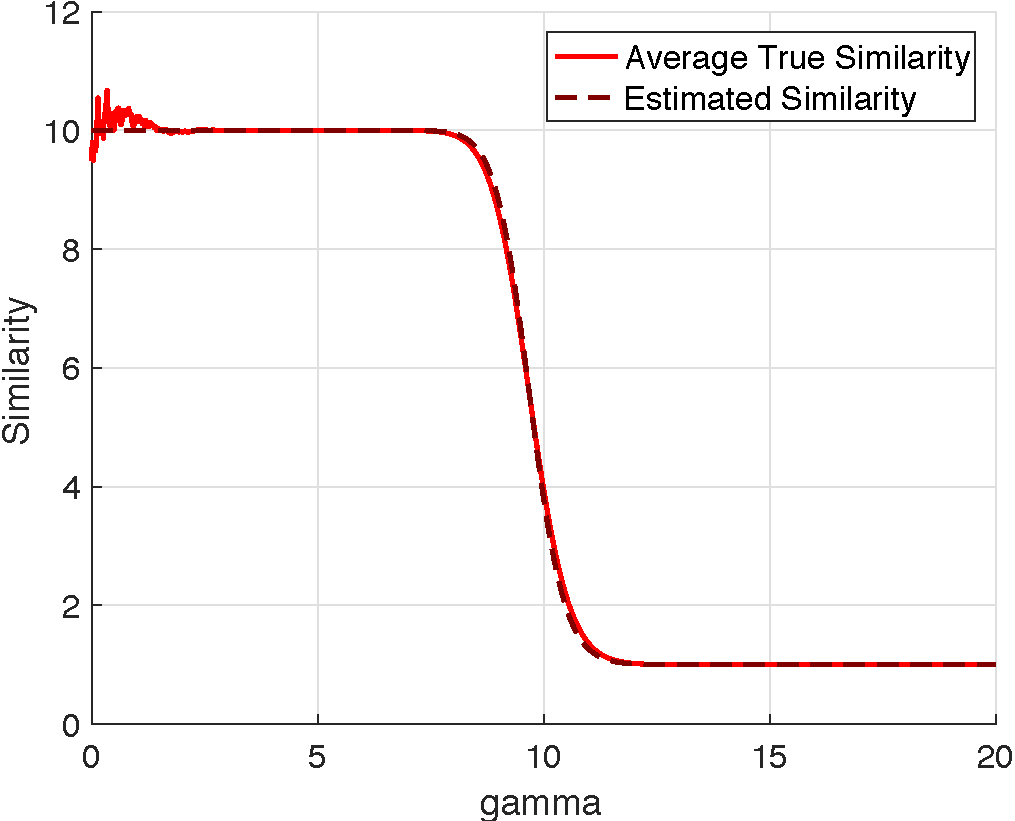
\includegraphics[width=\linewidth]{figures/ch_generic_approach/realVsEstimatedSimilarities_sb1}
      \caption{}
  \end{subfigure}
  \\[.5cm]
  \begin{subfigure}[b]{.6\textwidth}
      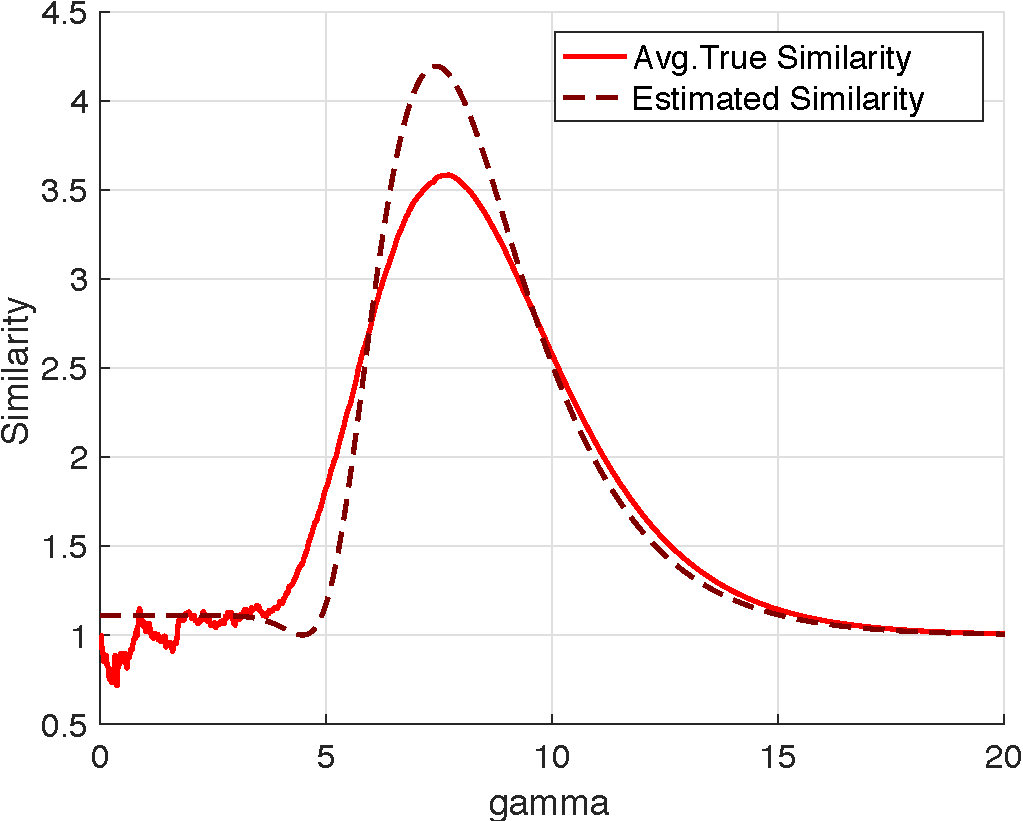
\includegraphics[width=\linewidth]{figures/ch_generic_approach/realVsEstimatedSimilarities_sb5}
      \caption{}
  \end{subfigure}
  \\[.5cm]
  \caption{Average vs. estimated similarity for $\sigma_{\mathrm{\B}}=1$ \textbf{(a)}, and for
    $\sigma_{\mathrm{\B}}=5$ \textbf{(b)}.}
  \label{fig:realVsEstimatedSimilarities}
\end{figure}
We see that the estimated similarity matches the average similarity relatively
well, especially for larger values of $\gamma$. Although the discrepancy grows
with the noise (which is natural due to the Taylor expansion used in the proof),
probably the most important thing to note is that the positions of the $\gamma^*$
computed based on $\hat S_\gamma$ and $\bar S_\gamma$ remain the same.

% \agcomm{till here}

% For $\sigma_{\mathrm{\B}}=5$, the situation is more difficult to analyze. However,
% Figure~\ref{fig:realVsEstimatedSimilarities}b shows that the maximum of the
% estimated similarity is larger than the estimated similarity at $\gamma=0$, and
% it also shows that the values $\gamma$ where the average and the estimated
% similarity, respectively, are maximized coincide well. Therefore the
% aforementioned problem of an empty intersection does not occur.

% As before we computed for both methods the
% intersection $\mathcal{C}_{\gamma^*}(X')\cap \mathcal{C}_{\gamma^*}(X'')$ and
% evaluated the resulting success probability using the definition
% in~\eqref{eq:uncert:prob_succ}. 
% Figure~\ref{fig:realVsEstimated} shows that for
% high noise, \tESIM\ has a higher chance to pick a \good\ solution than \tSIM\
% and \tMR\ which is not surprising because it has knowledge about the underlying
% process.
% \begin{figure}[t!]
%   \centering
%   \begin{subfigure}[b]{.85\textwidth}
%       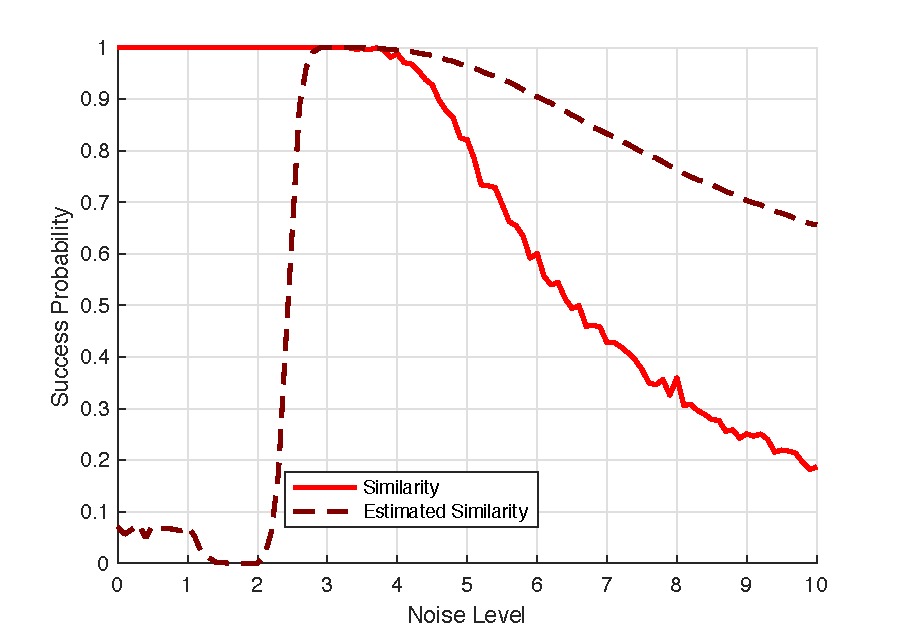
\includegraphics[width=\linewidth]{figures/ch_generic_approach/realVsEstimatedSuccessProbabilities}
%   \end{subfigure}
%   \\[.5cm]
%   \begin{subfigure}[b]{.85\textwidth}
%       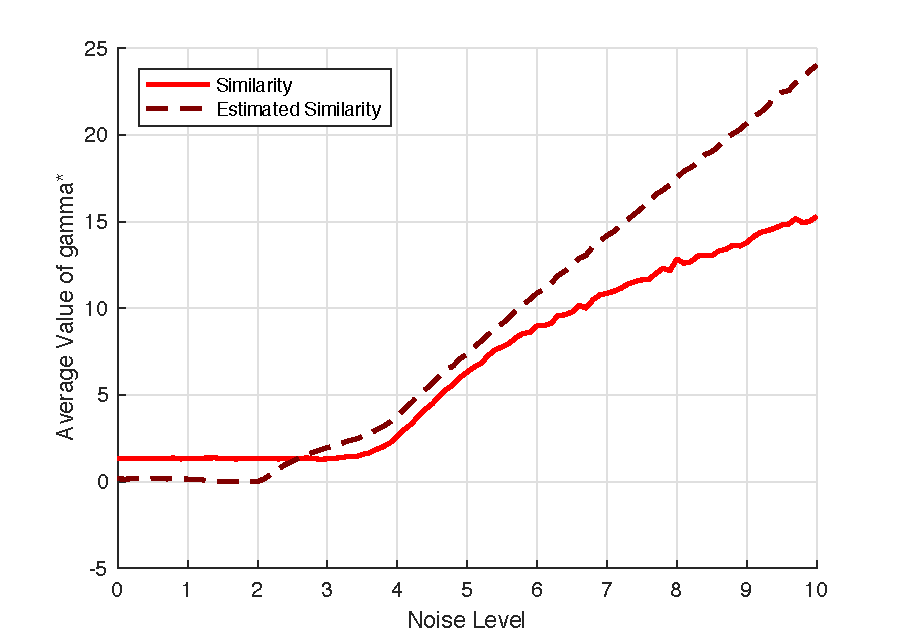
\includegraphics[width=\linewidth]{figures/ch_generic_approach/realVsEstimatedGamma}
%   \end{subfigure}
%   \\[.5cm]
%   \caption{Comparison of the success rates of \tMR\ and \tSIM\ with the one of
%     the estimated similarity (a), and a comparison of the values $\gamma^*$
%     that \tMR, \tSIM\ and \tESIM\ compute.}
%   \label{fig:realVsEstimated}
% \end{figure}

% The weak performance of the estimated similarity for small noise seems to be
% more surprising. To understand why this happens, consider
% Figure~\ref{fig:realVsEstimated}b\AGcomm{Fig ref broken} which shows the average value of $\gamma^*$
% that each method computes. Observe that for $\sigma_{\mathrm{\B}}<2.5$, the average value of
% $\gamma^*$ that the estimated similarity computes is below the one that
% \tMR\ computes, and since \tMR\ computes the
% smallest $\gamma$ for which the intersection of both $\gamma$-approximation sets
% is non-empty, the estimated similarity nearly always underestimates $\gamma$. To
% understand why this happens, we investigate the situation for $\sigma_{\mathrm{\B}}=1$ (low
% noise) and $\sigma_{\mathrm{\B}}=5$ (moderate noise). For each of the $\R=1000$ experiments,
% we compared the values of $\gamma^*$ that \tSIM\ computes with the
% ones of the estimated similarity. Figure~\ref{fig:realVsEstimatedPairs} shows
% the distribution of the points $(\gamma_\SIM^*,\gamma_\ESIM^*)$ where a point is
% red if \tSIM\ outperformed \tESIM, and green
% otherwise.
% \begin{figure}[t]
%   \centering
%   \begin{minipage}[t]{\textwidth}
%     \small
%     \centering
%     \includegraphics[width=.9\linewidth]{figures/ch_generic_approach/realVsEstimatedGamma_sb1}
    
%     (a)
%   \end{minipage}\\
%   \begin{minipage}[t]{\textwidth}
%     \small
%     \centering
%     \includegraphics[width=.9\linewidth]{figures/ch_generic_approach/realVsEstimatedGamma_sb5}
    
%     (b)
%   \end{minipage}
%   \caption{Each point corresponds to the outcome of one experiment, where the
%     $x$-coordinate denotes the value $\gamma^*$ computed by \tSIM\ and the
%     $y$-coordinate denotes the value $\gamma^*$ computed by \tESIM. A point
%     is red if \tSIM\ outperformed \tESIM, and green otherwise. The
%     experiments were performed for $\sigma_{\mathrm{\B}}=1$ (a), and for $\sigma_{\mathrm{\B}}=5$
%     (b).}
%   \label{fig:realVsEstimatedPairs}
% \end{figure}
% We see that for low noise, the estimated similarity nearly always
% underestimates $\gamma^*$. On the other hand, the choice of $\gamma^*$ for
% moderate noise is often better than the one by \tSIM. Hence, it
% seems that \tSIM\ is still too much influenced by the noise in the
% instances.

To summarize, we considered the expected similarity of two instances from the
same generator, and we derived an estimation for it that only depends on the
number of \good\ and \bad\ solutions, and on the respective cumulative density
functions. Our experiments showed that our estimation approximates the expected
similarity well when the noise is not too low. 
%
Our experiments also showed that the $\gamma^*$ that maximizes the estimated
similarity does indeed help to identify \good\ solutions. In particular,
choosing a solution from the intersection of the corresponding
$\gamma^*$-approximation is a promising way of robust solving. One of the
possible steps in this direction should be to analyze how many \good\ and how
many \bad\ solutions this intersection contains in expectation.

\section{Gibbs Relaxation of the Approximation Set-Based Approach}
\label{sec:gibbs_relaxation_of_sim}

\subsection{Approximation Sets with Gibbs Weights}
\label{sec:gibbs_relaxation_of_sim_weights}

\index{Approximation Set Coding!Gibbs relaxation}
\index{Gibbs relaxation|see{Approximation Set Coding}}
\nomenclature[D, 06]{$w^G_\beta(c, X)$}{Gibbs weights\nomnorefeq}%
\nomenclature[D, 06a]{$\beta$}{inverse temperature\nomnorefeq}%
\citet{conf/isit/Buhmann10}, in addition to the approximation set-based
approach, introduced its Gibbs-relaxed version which we give in this section.
The idea (we adapt it for the sake of notation alignment with the material of
this chapter) is as follows: using the maximum entropy principle
(Section~\ref{sec:background_max_entropy}) by~\citet{Jaynes82} from statistical
physics~\citep[see also][]{book/MezardM09}, for a real number $\beta \ge 0$, an
instance~$X$ and a solution~$c$, the Gibbs weight \index{Gibbs weights} of $c$
is defined as $w^G_\beta(c, X)
\coloneqq \exp(-\beta R(c, X))$. Now one computes a value $\beta^*$ that
maximizes
\begin{align}
  \label{eq:gibbs_realaxation}
  \beta^* = \arg \max_{\beta > 0}
    \log \biggl(|\C| \frac{\sum_{c\in\mathcal{C}}\big(w^G_\beta(c,X')\cdot w^G_\beta(c,X'')
      \big)}{\big(\sum_{c\in\mathcal{C}} w^G_\beta(c,X')\big)\cdot
      \big(\sum_{c\in\mathcal{C}} w^G_\beta(c,X'')\big)} \biggr),
\end{align}
\nomenclature[D, 06c]{$\beta^*$}{optimal inverse temperature}%
or, since the optimization goal is the same (see remark
after~\eqref{eq:similarity_maximization_objective}), maximizes the ratio
\begin{align}
  \label{eq:gibbs_similarity_maximization_objective}
  \beta^* = \arg \max_{\beta > 0}
    \frac{\sum_{c\in\mathcal{C}}\big(w^G_\beta(c,X')\cdot w^G_\beta(c,X'')
      \big)}{\big(\sum_{c\in\mathcal{C}} w^G_\beta(c,X')\big)\cdot
      \big(\sum_{c\in\mathcal{C}} w^G_\beta(c,X'')\big)},
\end{align}
and then samples a solution $c$ from the whole solution space $\mathcal{C}$ with
probability 
\[
  p_\beta(c) = \frac{w^G_{\beta^*}(c,X')\cdot w^G_{\beta^*}(c,X'')}{\sum_{c'\in
\mathcal{C}} (w^G_{\beta^*}(c',X')\cdot w^G_{\beta^*}(c',X''))}.
\]
We refer to this as the \textit{Gibbs relaxation of approximation set-based
approach}.

\subsection{Relation of Similarity and Gibbs Similarity}

Interestingly, the classical approximation set-based
approach~\eqref{eq:similarity_maximization_objective} and its Gibbs
relaxation~\eqref{eq:gibbs_similarity_maximization_objective} have a clear
relation: for a number $\gamma\ge 0$, an instance $X$ and a solution~$c$ we
define a 0-1-weight $w^\Ind_\gamma(c, X)$ that is $1$ if and only if $R(c,
X)\le R(c^\perp,X) +
\gamma$, and 0 otherwise. It is easy to see that
\begin{align}
  \label{eq:approximation_set_sum}
  |{\mathcal{C}_\gamma}(X')| &= \sum_{c\in\mathcal{C}} w^\Ind_\gamma(c, X')  \notag \\
  |{\mathcal{C}_\gamma}(X'')| &= \sum_{c\in\mathcal{C}} w^\Ind_\gamma(c, X'') \notag \\
  |{\mathcal{C}_\gamma}(X')\cap {\mathcal{C}_\gamma}(X'')| &= \sum_{c\in\mathcal{C}}
    \big(w^\Ind_\gamma(c,X')\cdot w^\Ind_\gamma(c,X'')\big).
\end{align}
\nomenclature[D, 06c]{$w^\Ind_\gamma(c, X)$}{indicator weights}%
With these equalities it follows that the objective of maximizing
$S_\gamma(X',X'')$ in~\eqref{eq:similarity_maximization_objective} corresponds
to the one of~\eqref{eq:gibbs_similarity_maximization_objective} in which the
0-1-weights $w^{\Ind}_\gamma$ are substituted for the Gibbs weights $w^G_\beta$.
%
Moreover, notice that $w^\Ind_\gamma(c,X')\cdot w^\Ind_\gamma(c,X'')=1$ if
and only $c\in {\mathcal{C}_\gamma}(X')\cap {\mathcal{C}_\gamma}(X'')$. Hence, sampling a solution from
$\mathcal{C}$ with a probability proportional to $w^\Ind_{\gamma^*}(c,X')
\cdot w^\Ind_{\gamma^*}(c,X'')$ corresponds to sampling a solution from
$\mathcal{C}_{\gamma^*}(X')\cap \mathcal{C}_{\gamma^*}(X'')$ uniformly at random.
%

Similar to the parameter $\gamma$ in Equation~\eqref{eq:simple}, the parameter
$\beta$ (called ``inverse temperature'' in statistical physics\footnote{Much
more on that will be given in Chapter~\ref{ch:free_energy}.}) 
\index{Inverse temperature} controls
the amount of solutions that are taken into account. For $\beta=0$, all
solutions have the same weight 1 (corresponding to the case $\gamma=\infty$ in
which the intersection contains every solution in $\mathcal{C}$), while for
$\beta\to \infty$ the distribution concentrates on the solutions with the
minimum joint cost. Hence, the parameter $\beta$
in~\eqref{eq:gibbs_similarity_maximization_objective} is by its semantics an
``inverse'' to the parameter~$\gamma$ in~\eqref{eq:simple}.

\subsection{Experimental Results}
\label{sec:gen_appch_gibbs_experiments}

\begin{figure}[t!]
  \centering
  \begin{subfigure}[b]{.49\textwidth}
      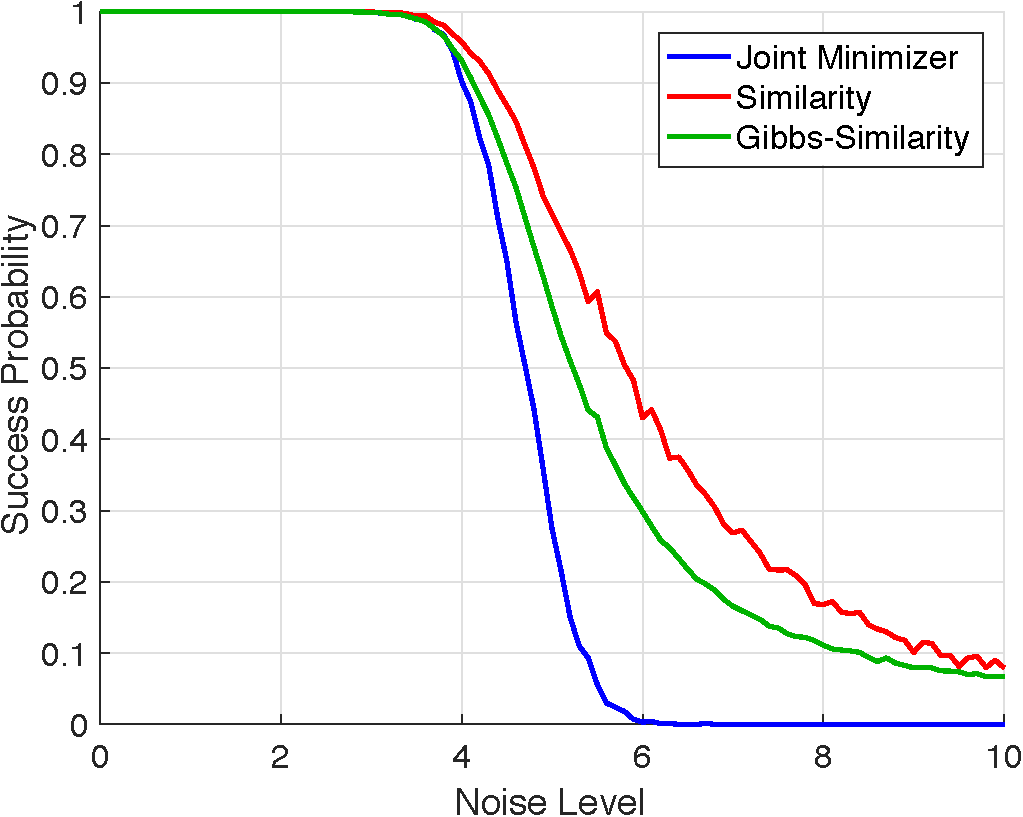
\includegraphics[width=\linewidth]{figures/ch_generic_approach/gnm_g50_b950_gibbs}
      \caption{$5\%$ of solutions are \good.}
      \label{fig:gnm_5_gibbs}
  \end{subfigure}
  \hfill
  \begin{subfigure}[b]{.49\textwidth}
      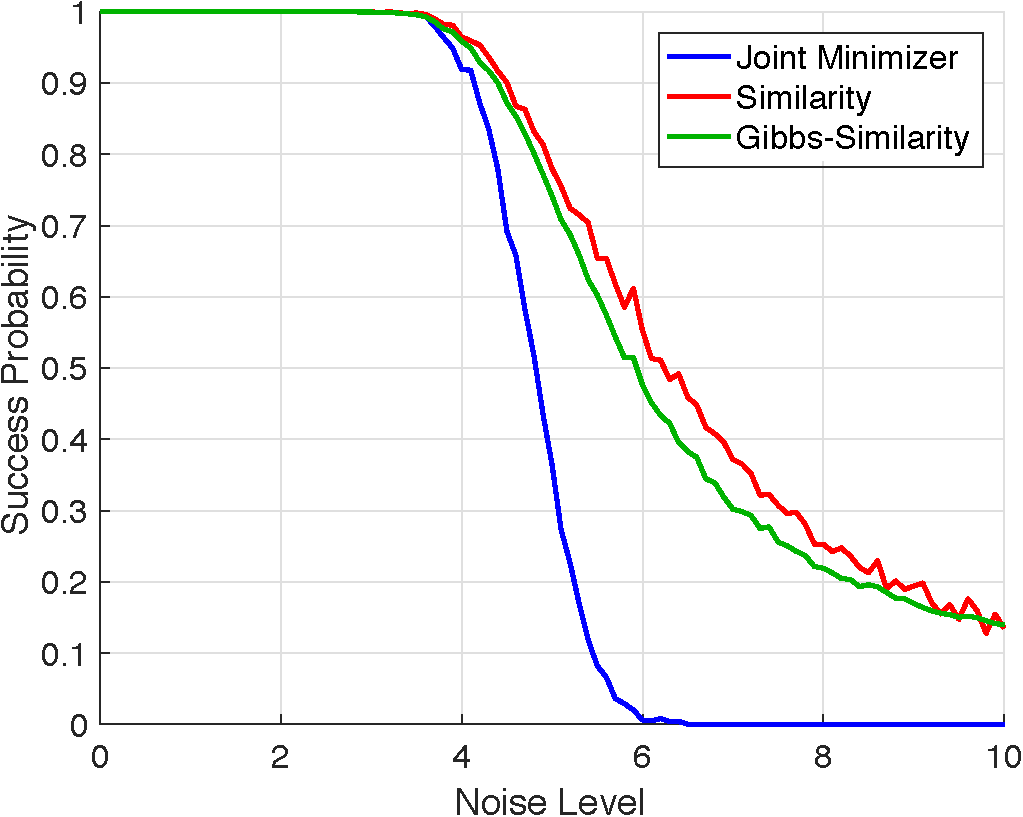
\includegraphics[width=\linewidth]{figures/ch_generic_approach/gnm_g100_b900_gibbs}
      \caption{$10\%$ of solutions are \good.}
      \label{fig:gnm_10_gibbs}
  \end{subfigure}
  \\[.5cm]
  \caption{Gibbs relaxation shows almost the same performance. Experimental
    results where $5\%$ \textbf{(a)} and $10\%$ \textbf{(b)}. Model and setting
    are the same as in Section~\ref{sec:proof_of_concept}.}
  \label{fig:gnm_gibbs}
\end{figure}

Since the Gibbs relaxation chooses every solution $c \in \mathcal{C}$ with a probability
proportional to $w^G_{\beta^*}(c, X')\cdot w^G_{\beta^*}(c, X'')$, we define its
success probability as
\begin{equation}
  P_\mathscr{A}^G(X',X'')
    \coloneqq \frac{\sum_{c \in \sgood} w^G_{\beta^*}(c, X')\cdot w^G_{\beta^*}(c, X'')}
      {\sum_{c \in \mathcal{C}} w^G_{\beta^*}(c, X')\cdot w^G_{\beta^*}(c, X'')}
\end{equation}
where $\beta^*$ is the value $\beta$ that
maximizes~(\ref{eq:gibbs_similarity_maximization_objective}). Notice that the
sums in the numerator and denominator are computed over different sets of
solutions. Notice that this formula is a full analogy
of~\eqref{eq:uncert:prob_succ}.

Figure~\ref{fig:gnm_gibbs} shows, under the same setting as in
Section~\ref{sec:proof_of_concept}, that the Gibbs relaxation provides yields
almost the same performance and thus can be considered as a viable variant
of the approximation set-based approach. This idea will be massively exploited 
in Chapter~\ref{ch:free_energy}.

\section{Discussion and Conclusion}
\label{sec:gen_appch_conclusion}

In this chapter, we introduced an approximation set-based approach to robust
optimization and justified it via a so-called Approximation Set Coding which
provides an information-theoretic background. Below, we will elaborate on some
points which are, in our view, highlighting its most interesting and/or
controversial properties.

\subsection*{Role of the logarithm}

Consider the comparison between the empirical ASC score~\eqref{eq:asc_mutual_information_formula}
\begin{equation*}
  \log 
    \frac{|\mathbb{\C}| \; |\Delta \mathcal{C}_\gamma(X', X'')|}%
      {|\mathcal{C}_\gamma(X')| \; |\mathcal{C}_\gamma(X'')|}
\end{equation*}
and the empirical similarity score~\eqref{eq:simple}:
\begin{equation*}
  \frac{|\mathcal{C}||{\mathcal{C}_\gamma}(X') \cap {\mathcal{C}_\gamma}(X'')|}
    {|{\mathcal{C}_\gamma}(X')||{\mathcal{C}_\gamma}(X'')|}.
\end{equation*}
Note that there is a difference in putting the logarithm in front of the 
ASC score. Although both have their maxima at the same $\gamma$, this logarithm
will be of essential importance later in Chapter~\ref{ch:free_energy} so
it is instructive to explain this difference.

The numerator and the denominator of the score can be seen as the
alternative and the null hypothesis, respectively, in statistical hypothesis
testing~--- the likelihood ratio test. One can view the usage of logarithm of
the likelihood ratio as a tool for ensuring asymptotic normality of estimators
in the case of weak coupling. For the main objective of this chapter, using the
logarithm had no special implications, since we were interested in the $\gamma^*$
which maximized score, but not in the score itself.

We should also note that the coding argument which we brought when deriving ASC
implies that logarithm allows to quantify the informativeness/capacity using \textit{bits}
(or \textit{nats}, depending on the type of the logarithm in use). This is 
turns the ASC score into the one which allows interpretable value~--- i.e. the one
answering ``how many bits of information can the model extract''.
\index{Nat (measure of information)}

\subsection*{Is the way of defining approximation unique?}
As one can see from the material of this chapter, the whole approximation
set-based approach rests on \textit{some notion} of closeness of the given
solution to the optimal one ($c^\bot$). We quantified this notion in terms of
parameters $\gamma$ or (in case of Gibbs approximation) $\beta$. But there
exists a whole zoo of other possible parametrizations, for example,
parametrizing by the step $t$ of a stepwise algorithm. However, we advocate the
point of view that such parametrization should yield a local topology around
each solution according to the following informal procedure:

\begin{enumerate}
  \item define certain measure of local closeness of solutions around the optimal;

  \item make an assumption: each solution \textit{is} the optimal solution for some
  input;

  \item local approximation topologies induced by the above create a ``cover''
  of the whole solution space; 
  \index{Topology}
  \index{Local approximation topology}

  \item derive conditions under which such a covering by local topology is can be
  turned into metric space (metrization theorems); \index{Metrization theorems}

  \item the above allows to create a uniform (i.e. non-local) closeness relation.
\end{enumerate}
This high-level roadmap gives some insight into the final goal of such a journey:
understand the structure of solution space in a problem-specific manner.

\subsection*{Are all solutions in the intersection created equal?}
Our method expects all solutions in the best approximation set intersection to
be equally desirable (e.g., equally good for a third, unknown instance). In some
cases, it might be useful to choose the solution based on some problem specific
criterion, e.g., choose the solution closest to the centroid of the intersection
set.

\subsection*{Will more input lead to better results?}
We mostly studied the two instance scenario because this is the minimum number
of instances necessary  to distinguish information from noise. Often, however,
more than two instances are available. The extension to multiple instances is
not immediately obvious.

There are several ways of addressing it: (a) first, one can break it into pairs
and average. This is how the framework is intended to be used in practice; (b)
second, one can derive a version of ASC for multiple agents. The latter approach
sounds much more interesting from the research prospective, as it is not clear
what would be the channel analogy in case of several agents (remember, in the
two instance scenario, we considered one data point as a codebook benchmark, and
the other as error problem generator). On can as well go in the direction of a
straightforward generalization of the similarity
formula~\eqref{eq:asc_mutual_information_formula}. In the course of our
research, some attempts have been made in that direction and they yielded
promising results.


\subsection*{Can we find efficient algorithmic solutions?}

The remark after Theorems~\ref{thm:simple}--\ref{thm:worst_case} tells that one
of the pitfalls of approximation set-based approach consists in computation of
the similarity score. While we used brute-force enumeration for our
proof-of-concept experiments, it would be of a great importance to find either
(a) analytical estimations for the similarity score or (b) efficient algorithms
for computing it.

In this chapter, we tackled case (a) and made an attempt to derive a very simple
analytical estimator, which uses the knowledge of the true distributions. This
assumption, of course, renders it useless in real cases, but allows usage of
plug-in estimators of the true distributions.

On a much higher level which uses less information about the true distributions,
the approach (a) will be tackled in Chapter~\ref{ch:free_energy}.

In specific cases, such as application to combinatorial algorithms, the approach
(b) can be used by utilizing combinatorial structure of the solutions. This will
be shown in Chapter~\ref{ch:mst}.

\subsection*{Similarity as a computational goal-specific measure}
An interesting side-result that we did not focus on in this chapter is the
expressiveness of instance similarity $S_{\gamma^*}$. In fact, it utilizes a
\textit{computational goal-induced} topology on the set of solutions. We bring
here a motivation which was best described in~\citep{jcss:2017}.
\index{Topology}
\index{Computational goal-induced topology}
For example, consider the problem of computing a shortest path between two given
vertices in a graph $G$. 
%
Having two instances $X'$ and $X''$ of this problem, one may attempt to measure
the similarity of these instances using certain structural information exposed to
us~--- e.g.,~the correlation coefficient or the Euclidean distance between the
vectors containing the edge weights.
\index{Euclidean distance}

However, if the instances differ a lot only in some weights which are usually
high and thus these edges that are never used in any nearly-shortest path, then
the similarity approach will correctly consider such examples as similar,
whereas for example the correlation coefficient will tell the opposite.
%
At the same time, if the computational goal was a maximum matching of edges
rather than the minimizing the weight cost, the similarity would regard the two
instances as significantly different.
%
This example highlights the need for a measure of \emph{similarity of instances
with respect to a computational goal}. This is performed by inducing a local topology
around each solution, and this topology depends only on the computational goal
and not on anything else.


\cleardoublepage

%!TEX root = ../gronskiy_phd_thesis.tex
\chapter[Minimum Spanning Tree Algorithms: Regularization by Stopping]{Minimum Spanning Tree
  Algorithms: \\ Regularization by Stopping}
\label{ch:mst}

\hfill
\begin{minipage}[t]{.75\textwidth}
\textit{``Besser ein Spatz in der Hand, als eine Taube auf dem Dach.'' \\
  (germ. ``A bird in the hand is worth two in the bush.'')} \\
  \hrule
  \vspace{.2cm}
  \hfill
  \textsc{--- Proverbs}
\end{minipage}

\section{Introduction}

\subsection{Motivation and Examples} 

\index{Minimum Spanning Tree}
\index{MST|see{Minimum Spanning Tree}}
Noise perturbed combinatorial optimization problems arise in various real-world
applications where problem instances are abstracted by weighted\footnote{We will
further utilize both the terms ``costs'' and ``weights'' in the same meaning.}
graphs with fluctuations in the weights. In this chapter, we
investigate the noisy Minimum Spanning Tree (MST) problems and their ability to
infer robust spanning trees. Examples of real-world applications of minimum
spanning trees come from various fields of human activity, such as
\emph{communication networks with delays} (optimizing message delivery times,
cf.~\citep{Bertsekas:1987}) or \emph{stock markets} (analyzing stock exchange
correlations, cf.~\citep{Sandoval:2012}), etc. All the applications require
trees with a high level of robustness to fluctuations since the quality of trees
is measured by expected costs. Wide real-world demand and applicability
stimulated extensive research on the robust minimum spanning trees
problem~\citep{Aron:2004, Kozina:1994, Sandoval:2012, Yaman:Karasan:Pinar:2001},
which addressed different aspects of the robust spanning tree setting, such as
development of algorithms, measuring algorithmic complexity, or comparing
robustness criteria.

In this chapter, we use an information-theoretic regularization approach
introduced in Chapter~\ref{ch:gen_appch} to analyse and validate MST algorithms
from the point of view of how well they can recognize (localize) the true
Minimum Spanning Tree under unknown noise in the graph instance. The validation
concept is developed for ``contractive'' algorithms that follow a step-by-step
strategy of shrinking the solution space until a single best solution is
identified.  This validation approach is based on the \emph{two-instance
scenario} \citep{Vapnik:1982} that requires statistical estimates to generalize
to test instances when the estimates have been inferred from a training
instance. For spanning trees, that means that they have to yield low costs on at
least two problem instances without being explicitly adapted to the test
instance.%%% JB: the reference to the IB method is obscure. We should
%%% reformulate it. 
Such regularization remains in the spirit of the \emph{information bottleneck
method}~\citep{Tishby:1999} in the sense that it tries to optimize the amount of
information that the algorithm might transfer from an artificial channel (see
below, Section~\ref{sec:ASReg}).
\index{Infromation bottleneck method}

%Suppose we need to construct a delivery
%network with minimal travel time along a given transportation system,
%where travel times along each road section fluctuate due to random
%transport delays caused by possibly unforeseeable events. Another 
%real-world application arises from stock financial markets,
%which exhibit strong correlations that can be
%modeled by a temporally evolving dependency graph. A minimalistic
%description of these correlations with a simple conditional
%independence structure requires to find a minimum spanning tree in
%such a noise contaminated graph (see~\citep{Sandoval:2012}). Both
%applications 

\subsection{Contributions and Outline of the Chapter}
\label{sec:mst_contribs}
As main contributions of this chapter, we
\begin{itemize}
  \item define a notion of contractive algorithm and give an general
  extension of the ASC regularization approach (introduced earlier in
  Chapter~\ref{ch:gen_appch}) for the case of stepwise contractive algorithmic
  problems. We call it Algorithmic ASC;
  \item provide a specialization of such extension to the case of three major
  algorithms solving the Minimum Spanning Tree (MST) problem, including the
  necessary tools to avoid brute-force enumeration known as a computational
  bottleneck of ASC;
  \item carry out experiments which justify usage of Algorithmic ASC score as
  a ranking tool related to expected localization error: higher Algorithmic ASC
  score yields lower error.
\end{itemize}

The chapter is outlined as follows. First, a related work overview is given in
Section~\ref{sec:mst_related_work}. Then, in Section~\ref{sec:mst_related_work}
we revisit those ingredients of ASC approach relevant for this chapter. A
comprehensive introduction into the original approximation set-based approach is
then given in Section~\ref{sec:asc_original}. Later, the main contribution is
made in Section~\ref{sec:mst_algorithmic_gen}, where we make a generalization of
the ASC to algorithmic problems, and Section~\ref{sec:applying_asc_to_mst} where
we directly apply it to Minimum Spanning Tree (MST) problem and three most
important algorithms solving it. Experimental results follow in
Section~\ref{sec:mst_results}. Finally, we discuss our findings in
Section~\ref{sec:mst_conclusion}.

\section{Related Work Overview} 
\label{sec:mst_related_work}

Literature entries on robust spanning trees vary by research purpose
(e.g.~algorithm complexity, robustness), adopted noise model
(e.g.~interval data), regularization strategy (regularizing by
pruning, graph preprocessing).  For example,
\citep{Yaman:Karasan:Pinar:2001} investigated graphs with edge weights
which are supposed to fall uniformly into a predefined interval. The
approach is based on regularization \emph{by preprocessing the graph},
which, in turn, involves eliminating selected edges and forcing other
edges to be included into the spanning tree.

\index{Pruning (tree)}
Regularizing an MST by \emph{pruning} as proposed
by~\citep{Sandoval:2012} identifies the presumably robust part of a
spanning tree. This goal is achieved by means of analyzing the
survival matrix constructed from adjacency matrices for training
minimum spanning trees.

Our approach is similar in that pruning (more precisely, optimal
stopping) is used as a regularization tool, but it rather aims at
\emph{analysis and comparison} of the algorithm's robustness by means
of such regularization. This approach also exhibits technical
differences from the mentioned work, relying only on \emph{two} data
instances, and it follows the spirit of learning theory with its goal
to analyse algorithms in a noise distribution independent way.

In Section~\ref{regularization_gen}, the general concepts of the
information-theoretic framework are given, as well as the
information-theoretic motivation. Then, in
Section~\ref{sec:mst_algorithmic_gen}, the application to stepwise algorithms
is discussed. The results and conclusion are summarized in
Sections~\ref{sec:mst_results} and~\ref{sec:mst_conclusion}, respectively.

\section{Approximation Set Coding Regularization}
\label{regularization_gen}

To make this chapter self-consistent, we first give a short overview of the approach
first introduced in Chapter~\ref{ch:gen_appch}, as well as of the
notation and terms used throughout this chapter.
\index{Regularization}

\subsection{Notation and Definitions}

Assume, there is a data instance $X$ given, for example
measurements in a data space $\mathcal{X}$, so that $X \in
\mathcal{X}$. In case of the MST problem, $\mathcal{X}$ is the set of
all possible combinations of the edge costs and $X$ is a particular realization
of such costs. Let $c$ denote a solution in a general set of solutions $\C$, so
that $c \in \C$. In case of the MST, $\C$ is the set of feasible spanning trees.

An optimization problem is defined by a cost (objective) function $R:
\C\times\mathcal{X}\rightarrow \mathbb{R}_{+}$ that assigns
each solution $c$ a real value $R(c,X)$. Furthermore,
$c^{\bot}(X) \in \arg\min_{c \in \C} R(c, X)$
denotes\footnote{In the context where it is clear what $X$ is, we
will omit the ``$(X)$'' in the notation: $c^\bot(X) \equiv
c^\bot$; $R(c,X) \equiv R(c)$; $\C_\gamma(X) \equiv
\C_\gamma$.} the minimum cost solution.

For the sake of referring to it in the rest of the chapter, we give here a
definition from Chapter~\ref{ch:gen_appch}:
\begin{definition}
\label{def:mst_ch_approximation_set}
For a given real number $\gamma \ge 0$, an approximation set is defined as follows:
\begin{equation}
  \mathcal{C}_\gamma (X, R) \coloneqq 
  \{c \in \mathcal{C} \mid R(c, X) - R^\bot(X) \le \gamma\},
\end{equation}
\end{definition}

In fact, it is desirable to find a \emph{robust set} of solutions
rather than a single solution, since we cannot trust the global
minimizer $c^\bot$ to achieve low costs on test instance due to noise
in the measurements. In this light, the sets $\C_\gamma(X)$ play
the role of a ``trade-off agent'' in the process of finding the robust
solution to optimization problem. This trade-off is 
%%% meant to be the one 
balancing the solution sets between overfitting ($\gamma = 0$) and underfitting (large
$\gamma$).
\index{Global minimizer}
\index{Overfitting}
\index{Underfitting}

%%%%%%%%%%%%%%%%% JB corrections up to here %%%%%%%%%%%%%%%%%

\subsection{Robust Solving via ASC Regularization}
\label{subsec:asc_regularization_crit}
Regularization by the Approximation Sets applies to a situation, when two data
instances $X', X'' \in \mathcal{X}$ are available and when both are generated by
injecting two noise realizations into the true data instance $X^0 \in
\mathcal{X}$ (see Section~\ref{sec:data_generation_model}). It is required for
both cases that the noise follows the same noise distribution: $X', X'' \sim
PG(X^0)$. In the spirit of statistical learning theory, we are interested in
distribution independent results since the distribution $PG(X^0)$ might be
unknown.

A robust solution to the noisy optimization problem $(\mathcal{X}, \C, R)$ is
obtained by the two-step process described in
Algorithm~\ref{alg:robust_solving_via_similarity}.

\begin{algorithm}[hb!]
\caption{Robust Solving via ASC Regularization}
\label{alg:robust_solving_via_similarity}
  \KwData{\\
  \quad two instances of the $X', X''$, \\ \\ 
  \quad cost function $R(c, X)$}

  \KwResult{Solution $c \in \C$.}

  {
    Find the optimal regularization parameter $\gamma^*$ that
    maximizes the log-ratio 
    % involving \emph{the first two data instances}:
    \begin{equation}\label{eq:mst_asc_ratio}
      \hat I_\gamma(X', X'') \coloneqq \log 
      \Bigl(
        \frac{|\C| \; |{\C}_{\gamma}(X') \cap {\C}_{\gamma}(X'')|}%
          {|\mathcal{C}_\gamma(X')| \; |\mathcal{C}_\gamma(X'')|}
      \Bigr),
    \end{equation}
  }

  {Choose a solution uniformly at random from the intersection of
        optimal approximation sets: $c \in C_{\gamma^*}(X') \cap
        C_{\gamma^*}(X'')$.}
\end{algorithm}

\myremark Note the difference of~\eqref{eq:mst_asc_ratio} with previously
defined~\eqref{eq:asc_mutual_information_formula}: dropping the 
expectation. This is perfectly legitimate in case when we have no access to the
problem generation distribution and have to replace the actual value by its
estimator.

\subsection{Information-Theoretic Basis for ASC Regularization}
\label{sec:ASReg}

Applying of ASC bases itself on the information-theoretic ground which uses
approximation sets $\C_{\gamma}(X)$ in a fictitious communication scenario.
This communication scenario involves sending and receiving a
\emph{transformation} $\tau\colon
\mathcal{X} \to \mathcal{X}$ that maps the data space onto
itself. We briefly recap the necessary information here: for a full
introduction, refer to Chapter~\ref{ch:gen_appch}
(Section~\ref{sec:communication_learning_stability}).

Communicating a true $\tau_{\mathrm{send}}$ is performed by sending ${\tau_{\mathrm{send}} \circ
X'}$ to the receiver, while the channel perturbs this ``message''
by substituting $X'$ with $X''$. Finally, the receiver obtains
$\tau_{\mathrm{send}} \circ X''$. The reader should note that $X'$ is known to
both sender and receiver.
\index{Sender}
\index{Receiver}
\index{Approximation Set Coding!Encoding and transmission}
\index{Approximation Set Coding!Decoding}

As the receiver 
%%% JB: receives
accepts $\tau_{\mathrm{send}} \circ X''$, it has has to distinguish the
fluctuations in $X''$ relative to $X'$ from the applied
transformation $\tau_{\mathrm{send}}$. Error free communication is guaranteed if the
receiver can identify the correct transformation $\tau_{\mathrm{send}}$ without
being deceived by these fluctuations.  The straightforward decoding
rule consists in finding the ``nearby'' transformation $\hat \tau$,
which maximizes the overlap between the received approximation set
$\C_\gamma(\tau_{\mathrm{send}} \circ X'')$ and the ``nearby'' approximation set
$\C_\gamma(\hat\tau \circ X')$.

The role of the codebook vectors is played by all such transformations
which enable us to cover the complete solution space $\C$
with approximation sets $\C_\gamma(\tau \circ X')$. Obviously,
$\gamma$ controls the number of such codebook vectors since for large
$\gamma$ we can only select few such sets to cover $\C$;
otherwise we risk decoding errors. The concept is analogous to
classical coding theory where every codebook vector defines the
``center'' of an ``error-correcting'' sphere, and the elements of this
sphere are \emph{indistinguishable} from the data transmission point
of view.
\index{Indistinguishable solutions|see{Solutions}}
\index{Solutions!Indistinguishable}

As derived in Section~\ref{sec:communication_learning_stability}, an
asymptotically vanishing error probability is achievable for coding rates
bounded by
%%
\begin{align}
  I_\gamma(X', X'') &= \Expct \hat I_\gamma(X', X'') \notag \\ 
  &=
  \Expct \log\left( \frac{|\C| \, |{\C}_{\gamma}(X') \cap
      {\C}_{\gamma}(X'')|}{|{\C}_{\gamma}(X')|
      \, |{\C}_{\gamma}(X'')|}\right), \label{eq:mst_ch_mutual_inf}
\end{align}
The estimator $\hat I_\gamma(X', X'')$ in (\ref{eq:mst_ch_mutual_inf}) measures
the total information content of a message.

For a fixed $\gamma$, a large overlap means that the evaluation of the first
dataset generalizes to the second dataset, whereas a small or empty intersection
indicates lack of generalization. The fraction of approximation set
cardinalities in (\ref{eq:mst_ch_mutual_inf}) measures stability of the solutions under
noise fluctuations.

The value $\Expct \hat I_{\gamma}(X', X'')$ is an estimate for the \emph{mutual
information} and, in analogy to information theory
(cf.~\citep[Ch.~7]{Cover:2006}), the \emph{approximation capacity} is defined as
$C \coloneqq\max_{\gamma}\Expct [\hat I_{\gamma}(X', X'')]$ (cf.
Definition~\ref{def:asc_score}). The expectation $\Expct$ is taken with respect
to the random variables $X', X''$. If the distribution $PG(X^0)$ is unknown then
we have to derive learning theoretic large deviation bounds based on the
empirical quantity $\hat I_{\gamma}(X', X'')$ and appropriate complexity
penalties.

In summary, maximizing the ratio~\eqref{eq:mst_asc_ratio} allows us to select the
optimal resolution for the solution set, and elements of this approximation set
are considered indistinguishable given the present noise process.

\section{ASC Regularization for Stepwise Algorithms}
\label{sec:mst_algorithmic_gen}

\subsection{Application to Stepwise Algorithms: Main Idea}

Direct application of ASC regularization requires
optimizing~\eqref{eq:mst_asc_ratio} w.r.t.~$\gamma$, which, in turn, amounts
to compute the cardinalities 
\begin{equation}
  |{\C}_{\gamma}(X') \cap {\C}_{\gamma}(X'')|, 
  \quad |{\C}_{\gamma}(X')|, 
  \quad |{\C}_{\gamma}(X'')|
\end{equation}
(cf. Definition~\ref{def:mst_ch_approximation_set}).  In general, computation or
at least estimation of these cardinalities requires to enumerate the elements of
$\C$ and to test if they belong to $\C_\gamma$. Such enumeration is
computationally hard, since $\C$ grows sometimes very fast (exponentially in
cases of some combinatorial problems).\footnote{This difficulty emerges as a
common bottleneck in many problem settings. We elaborated on it in
Section~\ref{sec:gen_appch_conclusion} of the previous chapter.}

For algorithms, these enumeration problems arise in a constraint form, i.e.,
\emph{the algorithm itself} might help to optimize this enumeration, eliminating
all those solutions that get ``out of consideration'' as the algorithm
progresses. In other words, some algorithms feature a step-by-step nature, and
they shrink the set of feasible solutions at each next step, ending up with the
optimal solution at the last step. Figure~\ref{fig:mst_contractive_algorithm}
illustrates this intuition. This contraction is very similar to the shrinkage of
approximation sets, as they shrink to the optimal solution as $\gamma$
decreases. The feasible sets induced by the algorithm often turn out to be
efficiently computable~-- and we will exploit this property of contractive
algorithms. 

\subsection{Contractive Algorithms and Their Approximation Sets}
\index{Contractive algorithm}We define the algorithmic approximation set at computational step $t$ as the set
of solutions that are still considered as potential answers to be returned by
the algorithm $\algo$. This generalized notion of an approximation set for
algorithm $\algo$ measures the statistical behavior of a specific algorithm
during its execution. 
\nomenclature[E, 05a]{$\algo$}{algorithm\nomnorefeq}%

\myremark Even if $\algo$ calculates the global minimum of the cost
function, the algorithm may not follow a gradient flow on that costs to
determine the global minimum.

\begin{figure}[ht!]
  \centering
  \includegraphics[width=\textwidth]{figures/ch_mst/contractive_alg}
  \\[.5cm]
  \caption{Illustration of a contractive algorithmic flow: the set of
    feasible (i.e. still possible) solutions contracts from step to step,
    shrinking to $c^\bot$ at the end of execution.}
  \label{fig:mst_contractive_algorithm}
\end{figure}

\begin{definition}
\label{def:contractive_algorithm}
  Assume that for a given data instance $X$ the stepwise execution of the
  algorithm $\algo$ evaluated on this instance can be expressed as a sequence of
  subsets of feasible solutions
  %%
  \begin{align}
    \algo(X) &= \langle A_0(X), \ldots, A_T(X)
    \rangle,
    \quad\text{where} \notag \\
  %%
    A_t(X) &\subseteq \C, \quad t = 0, \ldots, T, \qquad\quad
    \text{and} \notag\\
  %%
    A_0(X) &= \C \notag \\ 
    A_T(X) &= \{c^\bot\}.
  \end{align}
  \nomenclature[E, 05b]{$A_i(X)$}{algorithmic feasible set\mynomdef{def:contractive_algorithm}}%
  \nomenclature[E, 05b]{$T$}{total number of steps\nomnorefeq}%
  %%
  We call $\algo$ contractive, if $A_{t+1} \subseteq
  A_{t}$.  
\end{definition}

\begin{definition}\label{def:algorithmic_approximation_set}
  For a contractive algorithm it is natural to define an algorithmic
  $t$-approximation set as follows: $\C^\algo_t(X) \coloneqq A_t(X)$.
  \nomenclature[E, 05d]{$\C^\algo_t(X)$}{algorithmic $t$-approximation set\mynomdef{def:algorithmic_approximation_set}}%
  \index{Algorithmic!Approximation set}
  \index{Approximation set!Algorithmic|see{Algorithmic}}
\end{definition}

An example of such algorithm, as well as comprehensive illustration, will be
given in Section~\ref{sec:applying_asc_to_mst} and
Figure~\ref{fig:ch_mst_illustration}.

Speaking informally, the algorithmic $t$-approximation set is an approximation
set as defined in Definition~\ref{def:mst_ch_approximation_set}, but taken
w.r.t. the flow of a particular algorithm at update step $t$. The role of the
$\gamma$ parameter is now (in contrast to
Definition~\ref{def:mst_ch_approximation_set}) played by a discrete step
variable $t$ spanning from $0$ to $T$ (note that, generally, $T$ is not a
constant). All the other notions remain the same when adopting the new
definition of the approximation sets $A_t(X)$. For example, the following
defines the algorithmic ASC score:

\begin{definition}
As an analogy to~\eqref{eq:mst_ch_mutual_inf}, we will call the quantity
%%
\begin{align}\label{eq:alg_eq:mst_asc_ratio}
  I_t^\algo = \Expct \hat I_t^{\algo}( X', X'' ) 
    &\coloneqq \Expct \log\biggl( \frac{|\C| \, |{\C}^\algo_{t}(X') \cap
      {\C}^\algo_{t}(X'')|}{|{\C}^\algo_{t}(X')|
      \, |{\C}^\algo_{t}(X'')|}\biggr) \notag \\
    &\equiv \Expct \log \biggl(\frac{
      |\C|\; |A_t(X') \cap A_t(X'')|
    }{
      |A_t(X')|\; |A_t(X'')|
    }\biggr), 
\end{align}
\nomenclature[E, 05g]{$I_t^\algo$}{algorithmic ASC $t$-score}%
\nomenclature[E, 05ga]{$\hat I_t^\algo$}{empirical algorithmic ASC $t$-score}%
where $A_t(\cdot)$ are defined above, an algorithmic ASC $t$-score.
\index{Algorithmic!ASC score}
\index{Approximation Set Coding!Algorithmic|see{Algorithmic}}
\end{definition}
As in Chapter~\ref{ch:gen_appch}, we will distinguish between 
expected and empirical values.

\subsection{Algorithmic ASC Score and Optimal Stopping}
\begin{figure}[hb!]
  \centering
  \includegraphics[width=\textwidth]{figures/ch_mst/contractive_alg_opt_stop}
  \\[.5cm]
  \caption{The main question addressed in this chapter: which of the steps to
    choose for the optimal stopping.}
  \label{fig:mst_contractive_algorithm_opt_stop}
\end{figure}
As an empirical extension of the notions introduced in
Chapter~\ref{ch:gen_appch}, we claim that the algorithmic channel capacity
\begin{equation}
  C^\algo \coloneqq \max_{t = [0, \ldots, T]} I^\algo_{t} 
    = \max_{t = [0, \ldots, T]}\Expct [\hat I^\algo_{t}(X', X'')],
\end{equation} 
\nomenclature[E, 05gb]{$C^\algo$}{algorithmic approximation capacity}%
also referred as~\emph{algorithmic approximation capacity} or \emph{information
content}, equals the maximum amount of information which could be transferred
through a fictitious channel described in Section~\ref{sec:ASReg} (and, in more
detail, earlier in Section~\ref{sec:communication_learning_stability}), and
constrained to the specific algorithm (i.e., algorithmic approximation sets are
allowed). From the learning perspective, the algorithmic approximation capacity
shows how well the algorithm can filter out the noise (by $t$-optimization),
remaining robust to underfitting.
\index{Algorithmic!Approximation capacity}
\index{Optimal stopping}

In a full analogy with the approach of Chapter~\ref{ch:gen_appch}
(cf.\eqref{eq:asc_best_gamma}), one can find the optimal stopping time $t^*$ by
maximizing the algorithmic ASC $t$-score:
\begin{equation}\label{eq:mst_asc_best_step}
  t^* \in \arg \max_{t = [0, \ldots, T]} \hat \Expct I^\algo_t(X', X'').
\end{equation}
\nomenclature[E, 05g]{$t^*$}{optimal stopping time}%
We are going to use this approach as an optimal stopping criterion for the 
rest of the chapter (see Figure~\ref{fig:mst_contractive_algorithm_opt_stop}).

\myremark We will call this approach \textit{algorithmic ASC} opposed to the
original ASC approach developed in Chapter~\ref{ch:gen_appch}.
\index{Algorithmic!Approximation Set Coding}

\section{ASC Regularization for MST Algorithms}
\label{sec:applying_asc_to_mst}

\subsection{Major MST Algorithms}
In the rest of the chapter, we will consider the Minimum Spanning Tree (MST)
problem. Its formulation is as follows: given a weighted undirected graph $G =
(V, E)$, find a spanning tree of the minimum possible weight. \textit{Spanning
tree} is defined as a connected subgraph of $G$ without cycles, whose vertex set
equals $V$.
\index{Tree!Spanning}
\index{Spanning tree|see{Tree}}

There are several classical solutions to this problem, of which we will focus on
\textit{Prim's}, \textit{Kruskal's} and \textit{reverse-delete} algorithms. We
bring their definitions in a pseudo-code in
Algorithms~\ref{alg:prim_alg_pseudocode},~\ref{alg:kruskal_alg_pseudocode}
and~\ref{alg:rd_alg_pseudocode} and explain a verbal intuition behind them below.
\index{MST Algorithm!Prim's}
\index{MST Algorithm!Kruskal's}
\index{MST Algorithm!Reverse-delete}
\index{Prim's|see{MST Algorithm}}
\index{Kruskal's|see{MST Algorithm}}
\index{Reverse-delete|see{MST Algorithm}}


\begin{algorithm}[ht!]
\caption{Prim's Algorithm for finding MST}\label{alg:prim_alg_pseudocode}
\KwIn{undirected graph $G(V, E)$ with non-negative weights}
\KwOut{spanning tree with minimum total weight}
{initialize current tree $B = (V_B, E_B)$ by choosing first vertex: 
  $B \leftarrow (\{v^*\}, \emptyset)$\;}

\While{$V_B \ne V$ (not all vertices are in tree)}{
  {find the minimal edge $e_\mathrm{min} = (v, v_\mathrm{min})$ 
    from $B$ to the rest $G \setminus B$\;} 
  {add $e_\mathrm{min}$ to the tree $B$\;} }

\KwRet{current tree $B$}
\end{algorithm}

\begin{algorithm}[ht!]
\caption{Kruskal's Algorithm for finding MST}\label{alg:kruskal_alg_pseudocode}
\KwIn{undirected graph $G(V, E)$ with non-negative weights}
\KwOut{spanning tree with minimum total weight}
{initialize current tree $B = (V_B, E_B)$: $B \leftarrow (\emptyset, \emptyset)$ \;}

\While{$V_T \ne V$ (not all vertices are in tree)}{
  {find the minimal edge $e_\mathrm{min}$ such that: \\
    \quad a) $e_\mathrm{min} \not \in E_B$ and \\ 
    \quad b) $B \cup e_\mathrm{min}$ has no cycles\;} 
  {add $e_\mathrm{min}$ to the tree $B$\;} 
}

\KwRet{current tree $B$}
\nomenclature[E, 10a]{$G(V, E)$}{graph\nomnorefeq}%
\end{algorithm}

\begin{algorithm}[ht!]
\caption{Reverse-Delete Algorithm for finding MST}\label{alg:rd_alg_pseudocode}
\KwIn{undirected graph $G(V, E)$ with non-negative weights}
\KwOut{spanning tree with minimum total weight}
{initialize current graph $B = (V_B, E_B)$ with the input graph: $B \leftarrow G$
\;}

\While{$B$ is connected and yet not a tree}{
  {find the maximal edge $e_\mathrm{max}$ in $B$ such that: \\
    \quad deleting $e_\mathrm{max} $ does not disconnect $B$\;} 
  \If{no such edge found}{break\;}
  \Else{remove $e_\mathrm{max}$ from $B$\;} 
}

\KwRet{current tree $B$}
\end{algorithm}

\begin{figure}[th!]
  \centering
  \begin{subfigure}[b]{.48\textwidth}
      \includegraphics[width=\linewidth]{figures/ch_mst/mst_illustration_0}
      \caption{Step 2: candidate edges set is large, no restricted edges yet}
      \label{fig:ch_mst_illustration-0}
  \end{subfigure}
  \hfill
  \begin{subfigure}[b]{.48\textwidth}
      \includegraphics[width=\linewidth]{figures/ch_mst/mst_illustration_1}
      \caption{Step 3: candidate edges set is large gets smaller, restricted edges appear}
      \label{fig:ch_mst_illustration-1}
  \end{subfigure}
  \\[.5cm]
  \begin{subfigure}[b]{.48\textwidth}
      \includegraphics[width=\linewidth]{figures/ch_mst/mst_illustration_2}
      \caption{Step 4: candidate edges set is large gets even smaller, restricted edges build up}
      \label{fig:ch_mst_illustration-2}
  \end{subfigure}
  \hfill
  \begin{subfigure}[b]{.48\textwidth}
      \includegraphics[width=\linewidth]{figures/ch_mst/mst_illustration_3}
      \caption{Step 5: almost everything is restricted}
      \label{fig:ch_mst_illustration-3}
  \end{subfigure}
  \\[.5cm]
  \caption{Prim's MST Algorithm: freedom reduces as information
    grows. Edge weights are not shown (figure from the introduction recreated
    here for convenience).}
  \label{fig:ch_mst_illustration}
\end{figure}

\emph{Prim's algorithm} (``growing tree'' strategy) starts with a tree $B=(V_B,
E_B)$ on an empty set of edges $E_P$ and a starting vertex $v^{*}$. The
algorithm enlarges $E_B$, adding one edge $e_t$ at step $t$ (the first step
adds an edge incident to $v^{*}$), so that $B$ remains to be a tree, until $B$
becomes a spanning tree of $G$. It takes $T = n-1$ steps.

\emph{Kruskal's algorithm} (``connecting trees in a forest'' strategy) of
finding MSTs starts with an empty set of edges $E_B$. The algorithm adds
a minimal possible $e_t$ at the step $t$, not allowing cycles in $E_B$,
but yet not requiring $B$ to be connected at all times, until $B$ becomes a spanning tree
of $G$. It takes $T = n-1$ steps.

\emph{Reverse-Delete} (``reducing graph'' strategy) algorithm starts
with a graph on the full set of edges $B = G$ and shrinks it, removing one maximal edge
$e_t$ per step and keeping the graph
$B$ connected, until $B$ becomes a spanning tree. 
For a complete graph, it takes $T = n(n-1)/2 - n + 1$ steps.

\myremark All the three algorithms can be easily proven to reach the global
minimizer solution $c^\bot(X) \in \arg \min_c R(c, X)$.

\subsection{Counting Approximation Sets for MST}

\paragraph{MST algorithms are contractive} From the description of three
algorithms in the previous section one can see, that they all comply with the
Definition~\ref{def:contractive_algorithm} of a contractive algorithm, due to
the following line of reasoning. Since each of them yields a set (yet
\textit{not} an approximation set) of \textit{candidate edges} which still are
able to make it into the final tree:
\begin{itemize}
  \item in case of Prim's and Kruskal's: candidates are edges which are
    either already included or still can be included into $B$;
  \item in case of Reverse-Delete: candidates are edges which still remain (i.e.
    are no yet removed) in $B$.
\end{itemize}
To complete the reasoning, one should notice that an algorithmic approximation
set is exactly the set of spanning trees built on such candidate edges.

This concept is illustrated in Figure~\ref{fig:ch_mst_illustration}, where
several steps ($2$ to $5$) of the Prim's algorithm are shown. One can easily see
that as the algorithm flows, some edges are excluded from consideration (due to
no-cycle condition; shown in red) and hence less and less spanning trees remain
possible.

\paragraph{Computing cardinalities for MST} How can we calculate the
cardinalities of algorithmic approximation sets involved in the evaluation of
term~\eqref{eq:alg_eq:mst_asc_ratio}? Counting number of spanning trees for a
complete graph can be performed analytically via Cayley's
formula~\citep{Aigner2010}:
\newtheorem*{cayley_thm}{Theorem (Cayley's Formula for Spanning Trees)}
\begin{cayley_thm}
  The total number of labeled trees on $n$ vertices is equal to $n^{n-2}$.
  \index{Labeled tree|see{Tree}}
  \index{Tree!Labeled}
\end{cayley_thm}

\index{Cayley's formula}
However, Cayley's formula works only for complete graphs, while in our case, one
has to deal with a general case of counting trees on a non-complete subgraph
(candidate edges). In this work, we utilize the Matrix-Tree
Theorem~\citep[cf.][]{Harris:2008}. For a connected graph $G = (V,E)$, it
involves computing the adjacency matrix $M^G_{\mathrm{adj}}$, the degree matrix
\begin{equation}
  M^G_{\mathrm{deg}} = \mathop{\mathrm{diag}}(\deg{v_1}, \ldots,
\deg{v_n}),
\end{equation} 
and uses a notion of a cofactor:
\index{Degree matrix}
\index{Adjacency matrix}
\nomenclature[E, 07a]{$M^G_{\mathrm{adj}}$}{adjacency matrix}%
\nomenclature[E, 07b]{$M^G_{\mathrm{deg}}$}{degree matrix}%
\nomenclature[E, 07f]{$\mathrm{deg}(v)$}{degree of vertex}%

\begin{definition}
  Given an $n \times n$ matrix M, the $i,j$ cofactor of $M$ is defined to be
  $(-1)^{i+j} \mathrm{det}(M_{i, j})$, where $M_{i, j}$
  is the submatrix of $M$, where $i$-th row and $j$-th column are removed.
  \nomenclature[A, 00j]{$\mathrm{det}(\cdot)$}{determinant}%
  \index{Cofactor}
  \index{Matrix cofactor!see{Cofactor}}
\end{definition}

\newtheorem*{matrix_tree_thm}{Theorem (Kirchhoff's Matrix-Tree Theorem)}
\begin{matrix_tree_thm}
  The total number of labeled trees on a graph $G = (V,E)$ with adjacency matrix
  $M^G_{\mathrm{adj}}$, degree matrix $M^G_{\mathrm{deg}}$ is equal to (any) cofactor
  of the matrix $L = M^G_{\mathrm{deg}}- M^G_{\mathrm{adj}}$.
  \index{Kirchhoff's matrix-tree theorem}
\end{matrix_tree_thm}

%%The algorithm of finding the stepwise algorithmic
%%rate~\eqref{eq:mst_ch_mutual_inf} is thus the one described as
%%Algorithm~\ref{alg_mutual_inf}.
%%\begin{algorithm}
%%\caption{\textsc AlgApproxSetRatio}
%%\label{alg_mutual_inf}
%%\begin{algorithmic}
%%  \STATE $I\gets [\;]$ \COMMENT{the ratio~\eqref{eq:alg_eq:mst_asc_ratio} array}
%%  \STATE $P_1, P_2 \gets [\;]$ \COMMENT{candidate edges left at the
%%    current step (both for $X', X''$)} \FORALL{t = 1 \ldots
%%    T} \STATE $P_1 \gets P_1\setminus\{e_t(X')\}$ \STATE $P_2
%%  \gets P_2\setminus\{e_t(X'')\}$ \STATE\COMMENT{Now compute the
%%    cardinalities of aqpproximation sets} \STATE $N_1\gets$
%%  ComputeMatrixTreeCount($P_1$) \STATE $N_2\gets$
%%  ComputeMatrixTreeCount($P_2$) \STATE $N_{12}\gets$
%%  ComputeMatrixTreeCount($P_1 \cap P_2$) \STATE $I[t]\gets$
%%  ComputeRatio($N_1$, $N_2$, $N_{12}$)
%%\ENDFOR
%%\end{algorithmic}
%%\end{algorithm}

In our cases, applying the Matrix-Tree theorem to count cardinalities of algorithmic
approximation sets  ${\C}^\algo_{t}(X')$ and
${\C}^\algo_{t}(X'')$ is straightforward. Computing an intersection of two
algorithmic approximation sets ${\C}^\algo_{t}(X') \cap
{\C}^\algo_{t}(X'')$ is simple as well.

As the last step, it we find the optimal stopping step $t^* \in
\arg\max_t
\hat I^{\algo}_t( X', X'' )$ which maximizes the
ratio. The optimal stopping time $t^*$ then defines a
pruning operation on the solution space to make $\algo$ robust.

\subsection{Uniform Sampling an Optimally Stopped Spanning Tree}

Once the optimal stopping time $t^*$ is defined, we can sample from 
and intersection of two optimally-stopped algorithmic approximation sets 
${\C}^\algo_{t}(X') \cap {\C}^\algo_{t}(X'')$ using the Pr\"ufer encoding of
labeled trees. This purely algorithmic task, however, goes beyond the scope 
of this work and we thus leave it out.
\index{Pr\"ufer codes}

\section{Experimental Results} 
\label{sec:mst_results}
We will experimentally check that algorithmic approximation capacity is a consistent
measure of the information that can be extracted by an algorithm from
noisy data by means of optimal stopping.

\begin{figure}[!t]
\centering
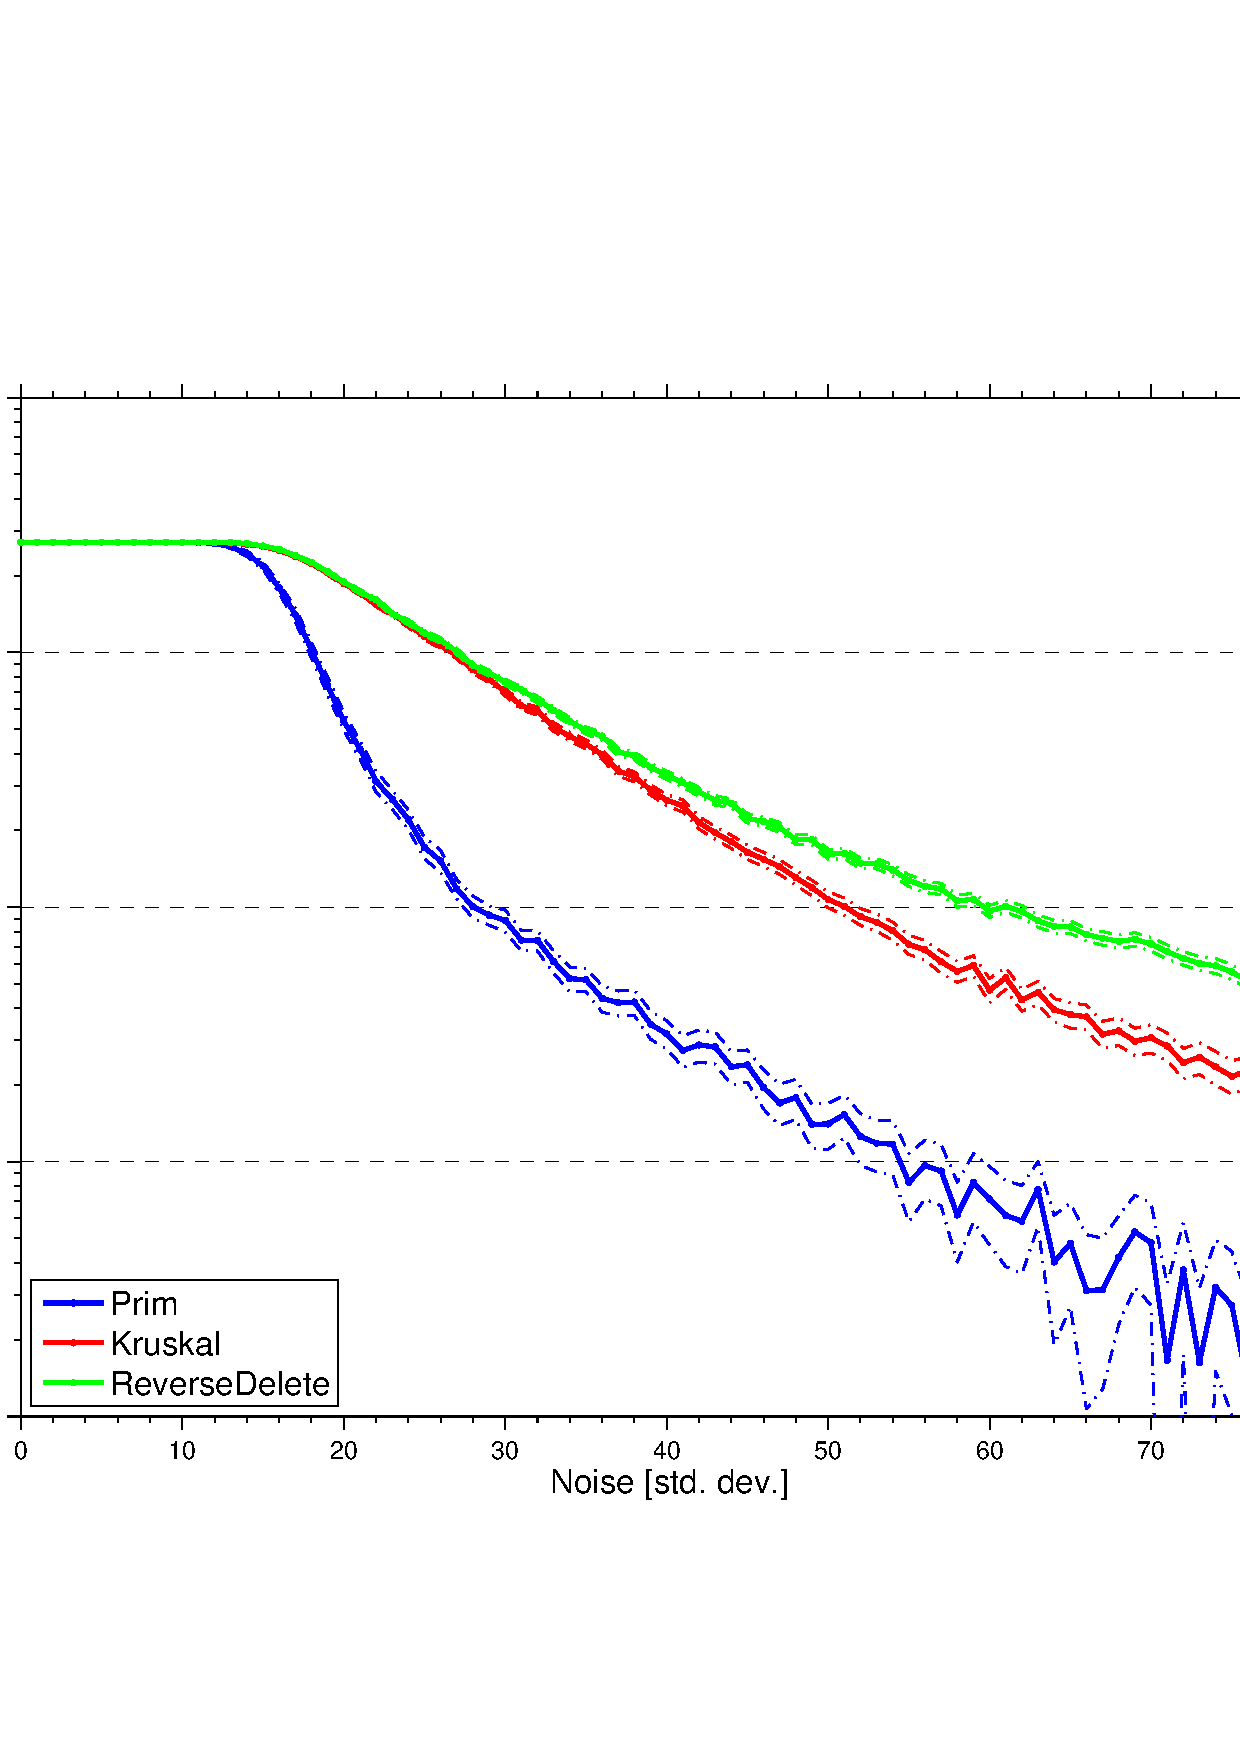
\includegraphics[width=.9\textwidth]{figures/ch_mst/gaus_inf_log}
\caption{Gaussian noise model: information content}
\label{fig:gaus_inf}
\end{figure}

\subsection{Experiment Setting: Gaussian Noise Model}
To investigate the general information-theoretic behavior of MST
algorithms in practice, we generate weighted complete graphs in a
hierarchical way. First, we generate a ``ground truth'' graph with
$n = 50$ vertices and with edges that are attributed by Gaussian weights,
sampled i.i.d. from a Gaussian distribution $\mathcal{N}(\mu_0 = 100,
\sigma_0^2 = 100)$.
Second, perturbed versions of this ground truth graph are then obtained by
adding Gaussian noise $\mathcal{N}(\mu = 0, \sigma^2)$ to the edge
weights for a given noise range $\sigma \in [0,  8\sigma_0]$.

In the experiment with approximation set-regularized algorithms we repeated the
experiment $400$ times to ensure the statistical significance of the
results. For some plots a semi-logarithmic scale was used for a better
visualization of small differences. Confidence intervals were also constructed
and plotted.

\subsection{Algorithmic Approximation Capacity Ranking of Algorithms}
\index{Ranking}
We plot the algorithmic information content $\max_t \Expct \hat
I_t^{\algo}(X', X'') $~(cf.~\eqref{eq:alg_eq:mst_asc_ratio}) for three algorithms (Figure~\ref{fig:gaus_inf}).
%%% JB: no new paragraph
At low noise levels (particularly $\sigma = 0$) all the three
algorithms exhibit the same information content, which is equal to
$\log_2{n^{n-2}} = 48 \log_2{50} \approx 270,9$ bits of information:
at zero noise, all the three algorithms choose the true MST out of
$|\C|$ possible spanning trees. For a complete graph,
Cayley's tree formula calculates the number of possible solutions as
$|\C| = n^{n-2}$.
%%% JB: In a noise-free setting, extracting the right tree corresponds
%%% to $\log_2{n^{n-2}} = 48 \log_2{50} \approx 270,9$ bits of
%%% information.    

The plot in Figure~\ref{fig:gaus_inf} provides a clear ranking of the three algorithms
w.r.t. their information content dependent on the noise level. A qualitative explanation 
which accounts for such ranking and 
clarifies the idea behind evaluating information content, is the
following:
%
%\begin{figure}[!t]
%\centering
%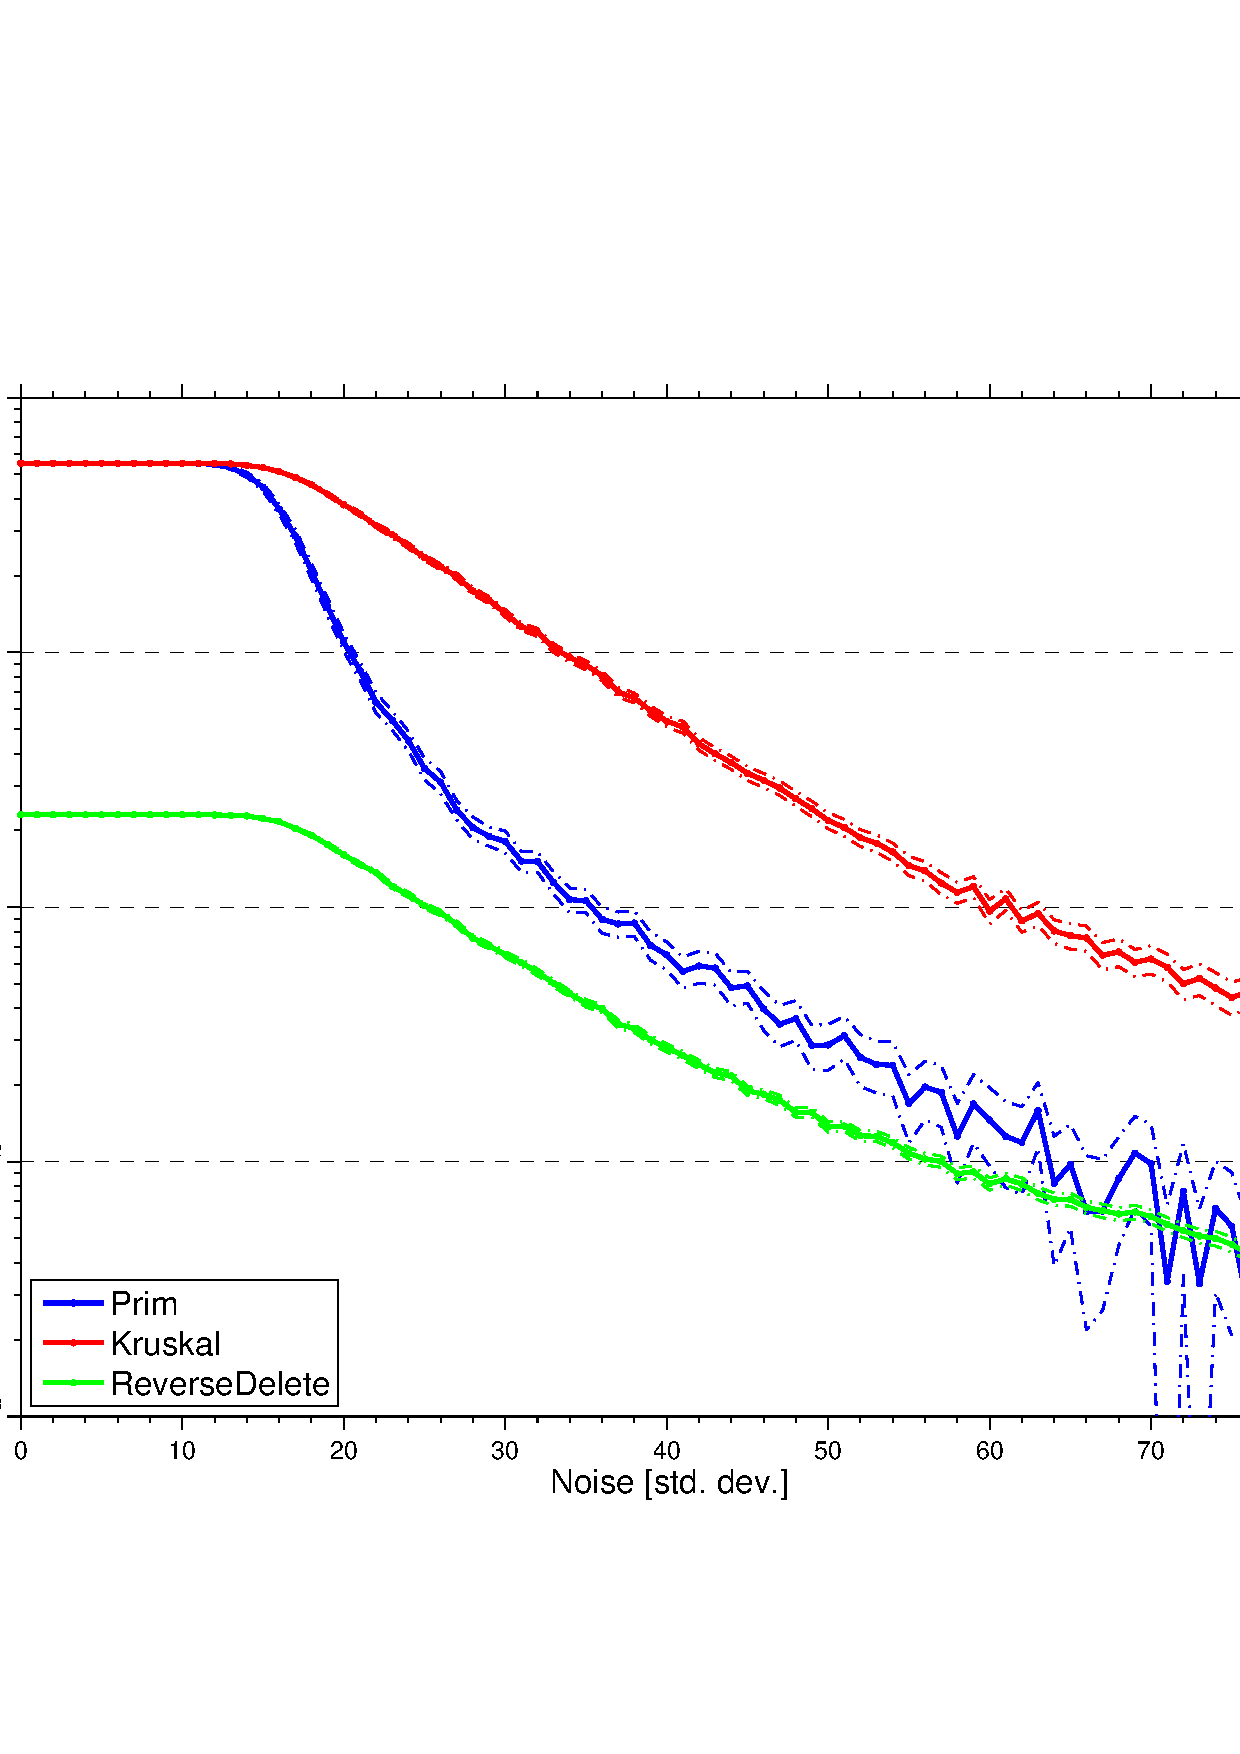
\includegraphics[scale=0.3]{figures/ch_mst/gaus_inf_step_log}
%\caption{Gaussian noise model: information content per step}
%\label{fig:gaus_inf_step_log}
%\end{figure}

\emph{Prim's algorithm} considers for addition only the edges which
are already connected to the tree built so far.  Among the not yet
considered edges there might be low cost edges which are more
efficient to be added in the beginning of the run rather than in the
end, thus making the information extraction inefficient from the point
of view of the algorithm dynamics.

\emph{Kruskal's algorithm} explores all the possible edges as
candidates for addition at each step, thus being less inclined to add
inefficient edges first and using the algorithm dynamics in a
efficient way. This gain is reflected by its increased informativeness
relative to Prim's algorithm.

\emph{Reverse-Delete algorithm} is more informative than Kruskal's,
since it efficiently discards all those edges which should not be
included in any approximate spanning tree. It pursues a strategy of
delayed decision making, that proved to be favourable also in other
situations of decision making under uncertainty.

\begin{figure}[!t]
\centering
\includegraphics[width=0.9\textwidth]{figures/ch_mst/gaus_loc_err_mod}
\caption{Gaussian noise model: localization error}
\label{fig:gaus_loc_err}
\end{figure}

The above insights are proven by the plot showing the stepwise
dynamics of logarithm of the cardinalities $|\C^\algo_t(X')|$, $|\C^\algo_t(X'')|$
(Figure~\ref{fig:gaus_as_card}). It visualizes the
fact, that as $t$ progresses, Prim's algorithm contracts for the
solution faster than Kruskal's, and both contract faster that the
Reverse-Delete one, which, in turn, forces earlier stopping and thus
leads to the worse performance. In fact, we can formulate an informal statement:
\begin{statement}
  Assume that at the step $t$ the algorithm exhibits the edge set $B$ defined
  above in Section~\ref{sec:applying_asc_to_mst}. Then the reduction of the
  amount of feasible spanning trees with edges in $B$ obtained by adding
  $e_{t+1}$ which is adjacent to $B$  (Prim) is higher than the reduction
  obtained by adding non-adjacent $e_{t+1}$ (Kruskal in general), and both are
  higher than the reduction obtained by deleting $e_{t+1}$ from $B$
  (Reverse-Delete).
\end{statement}

\index{Stepwise dynamics}
The plot in the Figure~\ref{fig:gaus_ratio_dyn} explains the discussed ranking
from the stepwise dynamics prospective. The algorithm, which reaches maximum of
mutual information earlier, is less informative in overall, and vice versa. This
behavior reflects a natural trade-off between early decision and informativeness of the
solution.

\subsection{Localization Error Ranking of Algorithms}

\index{Ranking}
The three given algorithms ``explore'' the solution set with different
dynamic behavior, extracting different amount of the information
about the true solution. This behavior is related to the localization error.

For the algorithmically ASC-regularized
(Section~\ref{subsec:asc_regularization_crit}) solution $\hat c$
we plot (Figure~\ref{fig:gaus_loc_err}) the localization error, which is
computed as $E(\hat c) = 1 - |c^* \cap \hat c| / |c^*|$, where straight brackets
denote the cardinality of edges.

\begin{figure}[!t]
\centering
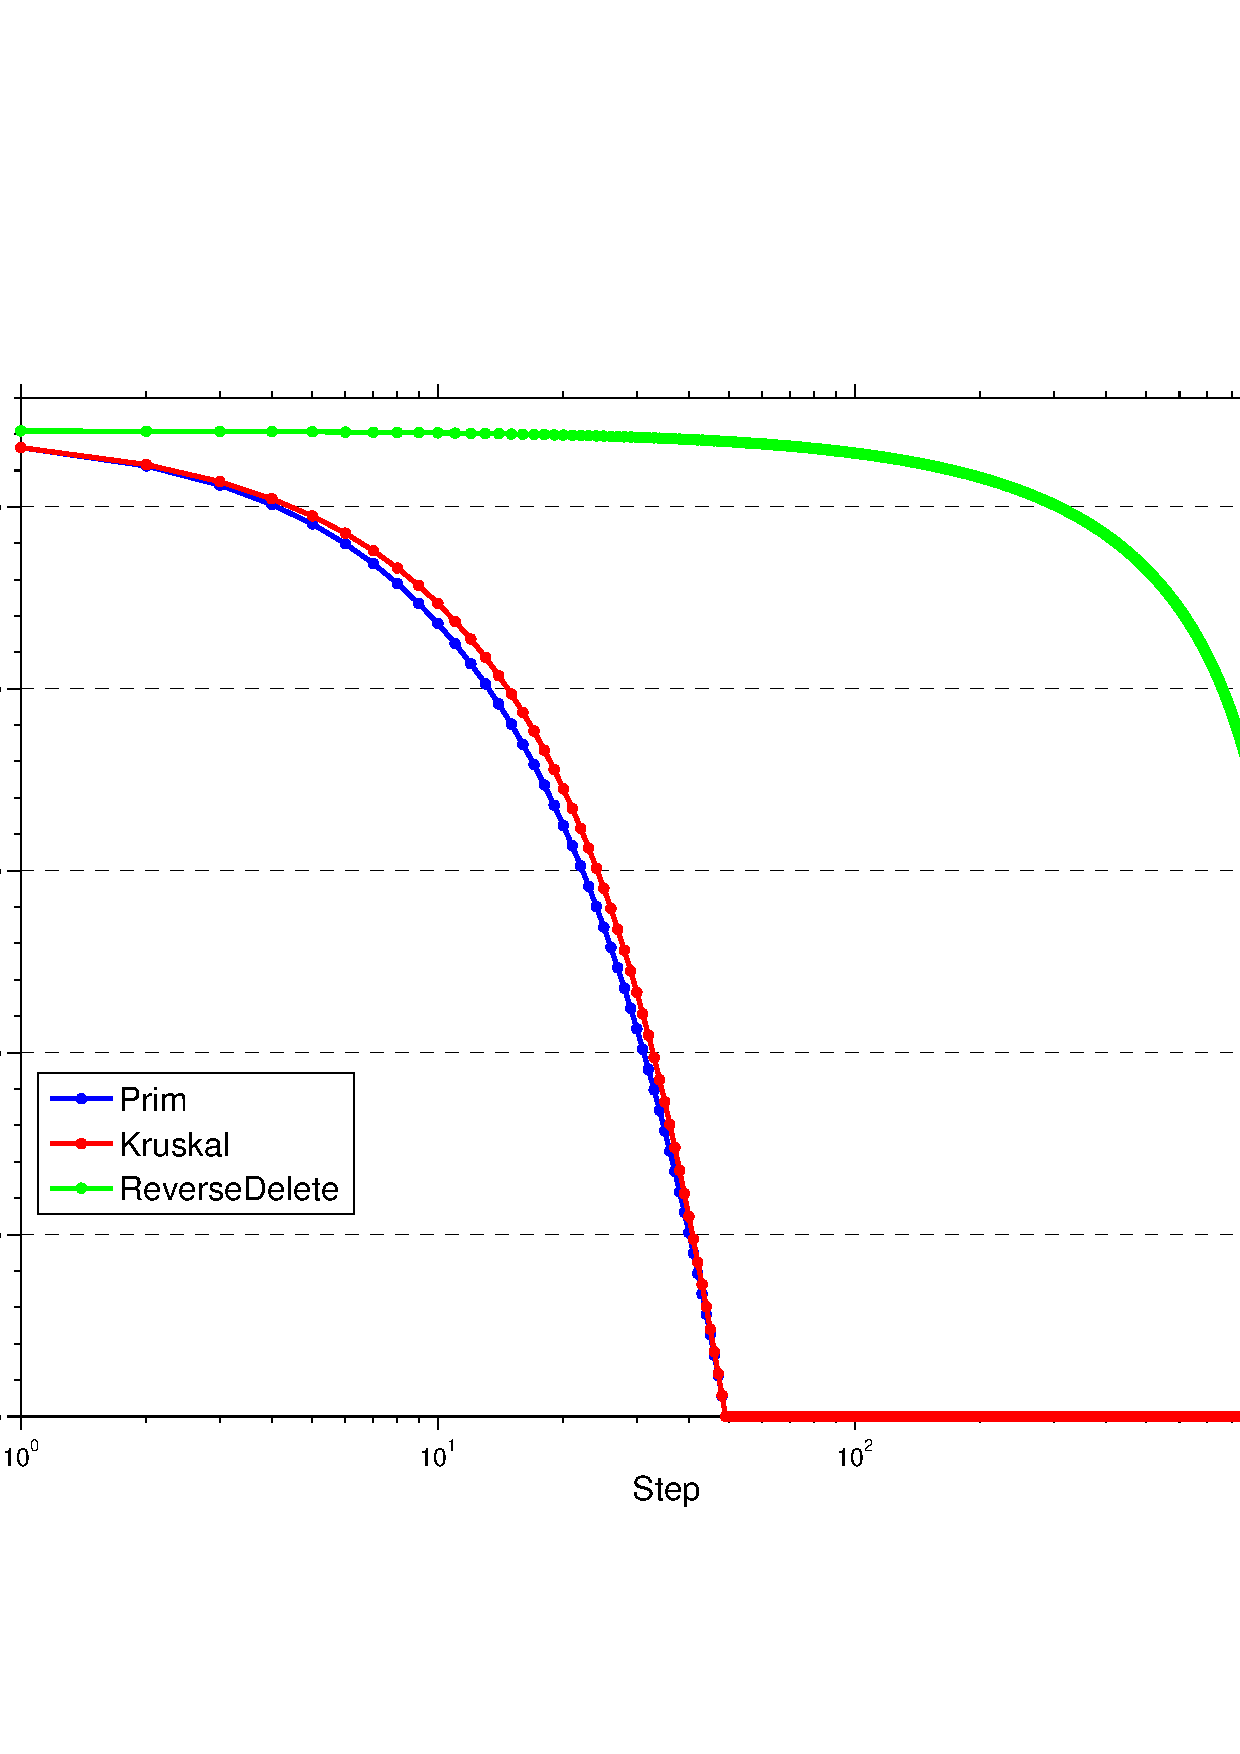
\includegraphics[width=.9\textwidth]{figures/ch_mst/gaus_as_card}
\caption{Gaussian noise model: stepwise approximation set log-cardinalities ($\sigma = 48$)}
\label{fig:gaus_as_card}
\end{figure}

\index{Localization error}
It can be seen from the figures, that the ranking of the three
algorithms according to their localization capability is in connection
with the information content ranking~--- the more informative
algorithm yields less error in localizing the true solution.

\begin{figure}[!t]
\centering
\includegraphics[width=.9\textwidth]{figures/ch_mst/gaus_ratio_dyn}
\caption{Gaussian noise model: stepwise algorithmic information defined in~\eqref{eq:alg_eq:mst_asc_ratio} ($\sigma = 48$)}
\label{fig:gaus_ratio_dyn}
\end{figure}
%
%\begin{figure}[!t]
%\centering
%\includegraphics[scale=0.3]{figures/ch_mst/gaus_as_intersection_card}
%\caption{Gaussian noise model: stepwise approximation set intersection log-cardinalities ($\sigma = 48$)}
%\label{fig:gaus_as_intersect_card}
%\end{figure}

\subsection{Algorithmic ASC vs. Original ASC}
\label{sec:aasc_vs_asc}

As the last experiment, we showed that the original ASC regularization (the one
via $\gamma$-parameter) works still better than algorithmic ASC and even beats
the Joint Minimizer (first introduced as a benchmark solution in
Chapter~\ref{ch:gen_appch}), which minimizes the average cost $R(c, X')+R(c, X'')$.
\index{Joint cost minimizer}

Due to the computation limitations of the original ASC~--- it yields enumerating
the whole set of spanning trees ($n^{n-2}$) for each step $t$ --- we could only
run the experiments for graphs with few vertices ($n = 6$).
Figure~\ref{fig:aasc_vs_original} shows that the original ASC remains
competitive with the Joint Minimizer solution, while algorithmic version shows
weak performance. This is not surprising and comes at a certain cost for which
we discuss in conclusion.

\begin{figure}[!t]
\centering
\includegraphics[width=.9\textwidth]{figures/ch_mst/gen_6_all}
\caption{Error plotted on the solutions obtained via original ASC
  (Chapter~\ref{ch:gen_appch} and algorithmic ASC (this chapter), as well as benchmarked on
  Joint Minimizer (Section~\ref{sec:aasc_vs_asc}).}
\label{fig:aasc_vs_original}
\end{figure}

\section{Discussion and Conclusion}
\label{sec:mst_conclusion}

\subsubsection{On the ASC-induced ranking of the algorithms}
The framework of approximation set coding is generalized from
the domain of models to the domain of algorithms in the
chapter. This framework enables us to apply an information-theoretic
regularization and quality assessment principle to algorithms,
and, in particular, to a minimum spanning tree problem with noisy
graphs as input.

We interpreted the results of the quantitative analysis of the
algorithms in a qualitative way, binding the strategy of the algorithm
to its information content, showing consistency and agreement with the
localization capability of the algorithm.

The ranking of the quantities plotted in
% Figure~\ref{fig:gaus_inf},~\ref{fig:gaus_loc_err},~
% \ref{fig:gaus_as_card},~ \ref{fig:gaus_ratio_dyn}
Figure~\ref{fig:gaus_inf}--\ref{fig:gaus_ratio_dyn}
support the following conjecture.
\begin{conj}
  The information content of contractive algorithms applied to the
  same problem establishes a ranking among them. This ranking is
  consistent with the average localization error of these algorithms.
\end{conj}

A possible way of investigating this relation is a rigorous analysis of the
approximation set dynamics using the mentioned Matrix-Tree theorem.
Although we utilized the simplest model of Gaussian noise,
independent on separate edges, there exists evidence, which
allows us to expect the same consistent results for a \emph{structured}
noise setting, when the edges of the graph are impacted by the noise
in a complex way, involving the statistical dependence of the noise
ingredients and other degrees of the noise model complexity.

\subsubsection{Algorithmic ASC vs. original ASC}

Should one use algorithmic approximation approach of this chapter or the
original $\gamma$-approximation approach form Chapter~\ref{ch:gen_appch}? In
this section, we address a question on whether the optimal stopping rule derived
by algorithmic ASC can compete with the original ASC (we initiated this discussion
in Section~\ref{sec:aasc_vs_asc}).

In fact, these two approaches serve quite different purposes and feature
different highlights. The original $\gamma$-parametrized ASC regularization
works in conjunction with the optimization goal $R(c, X)$, while its algorithmic
version makes use of algorithm-specific \textit{flow}. Although the algorithm
finds the same global optimizer as a bare $R(c, X)$-minimization procedure, the
structure of approximation sets if very different. Below, we list the main
points of difference:
\begin{itemize}
\item The original ASC relates to the continuous parameter, while algorithmic ASC
works with a discrete steps. This yields different power of resolution at which 
we coarse-grain the solution set $\C$. For original ASC, this resolution power 
is higher (it can allow much smaller step between approximation set sizes), while 
for algorithmic ASC it fully depends on the algorithm.

\item Original ASC is hard to apply computationally, since it boils down to 
computing and enumerating approximation sets. For algorithmic ASC, it is easier
to derive a problem-specific procedure which makes it \textit{orders of
magnitude} faster. For example, in the MST case, we utilized the Matrix-Tree
theorem and computed the cardinalities analytically at each step!
\end{itemize}

Hence, the trade-off between the power of resolution and the computational 
power exists and should be addressed in each special case.

\subsubsection{General notes on the ASC approach to algorithms}

From the statistical physics perspective, a contractive algorithm can be
considered as a process, where the temperature decreases step by step, and thus
``freezes'' the solution space, until finding the optimal solution. The
survey~\citep[Sec.~3.2]{Merhav:2010} discusses the connection between such a
coding framework and statistical physics. This connection \citep{JB:ISIT:2010}
inspires us to explore the dynamics of the algorithm from a generalization point
of view and to relate it to the information theory~\citep{Merhav:2010}.

We will consider the statistical physics viewpoint on the ASC regularization in the next
chapter.
\cleardoublepage

%!TEX root = ../gronskiy_phd_thesis.tex 
\chapter[Combinatorial Optimization: Regularization by Free Energy]{%
  Combinatorial Optimization: \\ Regularization by Free Energy}
\label{ch:free_energy}

\hfill
\begin{minipage}[t]{.75\textwidth}
\textit{``Tout cela, Maxwell et Boltzmann l'ont expliqué, mais celui qui l'a vu
plus nettement, dans un livre trop peu lu parce qu'il est difficile à lire,
c'est Gibbs dans ses principes de la Mécanique Statistique.''} \\[.2cm]
\textit{(fr. ``All this, Maxwell and Boltzmann have explained, but the one who saw it
in the cleanest way, in a book that is too little read because it is difficult
to read, is Gibbs, in his `Principles of Statistical Mechanics'.'')} \\
\hrule
\vspace{.2cm}
\hfill
\textsc{--- Henri POINCARÉ}, ``La valeur de la science''
\end{minipage}

\section{Introduction}

Most real world combinatorial optimization problems are affected by noise in the
input data, thus behaving like large disordered particle systems, e.g. spin
glasses. And similar to large physical systems, they optimize a certain functional
(energy, cost function). 

In this chapter, we will work with two notions arising from this analogy:
\textit{Gibbs distribution} and \textit{free energy}. We address two
interrelated questions connected to these notions: first, we provide rigorous
asymptotic computation of the matching upper and lower bounds on the free energy
(for two disordered combinatorial optimization problems, the sparse Minimum
Bisection Problem, sMBP, and Lawler's Quadratic Assignment Problem, LQAP). We
show that the free energy exhibits phase transitions equivalent to that of 
Derrida's Random Energy Model (REM). Then, the obtained free energy asymptotics
leads to the second contribution of this chapter: theoretic justification of the
Gibbs relaxation of ASC introduced earlier in Chapters~\ref{ch:gen_appch}
and~\ref{ch:mst}. We perform it by introducing the \textit{Gibbs posterior
agreement}, which is, in simple terms, a measure of stability of the Gibbs
distributions in case when the cost function fluctuates. Additionally, we carry
out experiments which support phase transition findings and conjecture further
extension of the theorems proven in the chapter.

\subsection{Notation}
\label{sec:free_setting_notation}

\myremark Before reading this section, we advise the reader to briefly revisit 
the notation of Section~\ref{sec:background_disordered_systems},
Definition~\ref{def:optimization_problem_definition} for notational analogies.

We consider combinatorial optimization problems that can be formulated as
follows (for explanation see Fig.~\ref{fig:notation_explained}): let $n$ be some
integer determining the size of the problem (e.g., number of vertices in a
graph, size of a matrix, etc.), and $\S_n$ a finite set of objects (e.g., set of
edges, elements of a matrix, etc). Working in the spirit
of~Section~\ref{sec:background_disordered_systems} and under the rigorous
notation of Definition~\ref{def:optimization_problem_definition}, we then let
$\data$ denote some random input to the problem (data).
\nomenclature[F, 00a]{$n$}{combinatorial problem size\nomnorefeq}%
\nomenclature[F, 00d]{$\S_n$}{set of base objects\nomnorefeq}%

\begin{figure}[htbp]
  \centering
  \noindent\includegraphics[width=.9\textwidth]{figures/ch_free_energy/solution_set_illustration} 
  \\[.5cm]
  \caption{Illustration of the notation: each of solutions (examples shown in the figure
  are $c_i$, $c_j$, $c_k$) includes $N$ (in the figure $N = 7$) objects from the
  underlying set $\S_n$. The cost function of a solution is the sum of weights
  assigned to the objects, which belong to that solution.}
  \label{fig:notation_explained}
\end{figure}

\nomenclature[F, 05a]{$\C_n$}{set of solutions\nomnorefeq}%
\nomenclature[F, 05d]{$c \in \C_n$}{solution\nomnorefeq}%
\nomenclature[F, 05h]{$\S_n(c) \subseteq \S_n$}{base objects in colution\nomnorefeq}%
\nomenclature[F, 05k]{$X$}{random source\nomnorefeq}%
\nomenclature[F, 05k]{$w_i(\data) = W_i$}{weight of object\nomnorefeq}%
Define $\C_n$ as a finite set of all feasible solutions (e.g.
bisections of a graph), and $\S_n(c) \subseteq \S_n$,
$c\in\mathcal{C}_n$, as a finite set of objects belonging to the
feasible solution $c$ (e.g., set of edges belonging to a bisection).
Let $w_i(\data) = W_i$, $i \in \S_n$, be the weight assigned to the
$i$-th object. In this chapter we consider optimization problems for which the cost
function and optimization task are defined as follows:
\begin{equation}
  \label{eq:cost_function_erm}
  R(c, X) = \sum_{{i} \in \S_n ( c )} w_i ( \data )\quad \text{and} \quad
  c^\bot(X) \in \arg \min_{c \in \C_n} R(c, X).
\end{equation}

\nomenclature[F, 05m]{$m$}{solution set cardinality\nomnorefeq}%
\nomenclature[F, 05o]{$N$}{solution size\nomnorefeq}%
We also denote the cardinality of the feasible set as $m$
(i.e., $m \coloneqq |\C_n|$) and the cardinality of $\S_n(c)$ as $N$ for all $c
\in \C_n$ (i.e., solution size $N \coloneqq |\S_n(c)|$). In this chapter, we
focus on optimization problems in which $\log m=o(N)$ holds
true~\citep[see][]{ws95optimization}.%%% JB: Explanation why we call these problems parameter rich. 
We call these optimization problems \emph{parameter-rich} since the
log cardinality scales sub-linearly with the number $N$ of objects that
belong to a solution~$c$.
\index{Optimization problem!Parameter-rich}

\subsection{Motivation: ASC Gibbs Relaxation via Free Energy}
\label{sec:free_boltzmann-distr-validation}

\paragraph{Gibbs relaxation of ASC} As mentioned in the introduction, most real
world combinatorial optimization problems are affected by noise in the input
data $X$. Therefore, they behave like large disordered particle systems, e.g.,
random networks or spin glasses. Like physical systems, they optimize an
application-dependent functional (cost function), and their solutions are
characterized by some \textit{posterior
distribution} $p(c|X)$ given the data $X$. In view of this stochastic setting,
one can ``robustify'' the solution by the maximum entropy method.  In the framework of maximum entropy, it is well
justified (see \citet{mezard84tsp}) to use Gibbs distributions, known also as
\textit{Gibbs posteriors}, for the posterior distribution $p(c|X)$ leading to a
novel pipeline presented in Fig.~\ref{fig:posterior-explanation} (lower) as
opposed to the standard one (upper).
\index{Gibbs relaxation|see{Approximation Set Coding}}
\index{Gibbs posterior}
\index{Posterior distribution|see{Gibbs posterior}}


\begin{figure}[htbp]
  \centering
  \noindent\includegraphics[width=.9\linewidth]{figures/ch_free_energy/posterior-distribution-explanation}
  \\[.5cm]
  \caption{Standard risk minimization (upper) solution and a solution obtained
  via sampling from approximating posterior distribution (lower).}
  \label{fig:posterior-explanation}
\end{figure}

\myremark The following is the elaboration of the Gibbs ASC relaxation first
introduced very briefly in Chapter~\ref{ch:gen_appch}. Although we give all the
necessary definitions below, we still advise the reader to revisit the
respective Section~\ref{sec:gibbs_relaxation_of_sim_weights}.

\begin{definition}
  Suppose we are given an optimization problem defined by a cost
  function $R(c,X) \in \mathbb{R}$, where $c$ is a solution from the
  finite solution space $\C$ and $X$ is a random data instance.  Then
  the \textbf{Gibbs posterior distribution} $p_\beta(c | X)$ defined
  as 
  \begin{align}\label{eq:GibbsDistr}
    p_\beta(c|\data) &=\frac{1}{Z(\beta, X)} \exp(-\beta R(c, \data))
      \quad\text{with} \notag \\
    \quad Z(\beta, \data) &= \sum_{c^\prime\in \C} \exp(-\beta R(c^\prime, \data))\,.
  \end{align}
\end{definition}
\nomenclature[F, 07a]{$p_\beta(c \vert \data)$}{Gibbs posterior}%
\nomenclature[F, 07c]{$Z(\beta, \data)$}{random partition function}%
\nomenclature[F, 07f]{$\beta$}{inverse temperature}%
The term $Z(\beta, X)$ is known as the \textit{partition function}. The Gibbs
distribution is parameterized by a parameter $\beta$  which is called
the \textit{inverse temperature}. For any $\beta$ the Gibbs posterior assigns the highest
weights to those solutions that have the smallest costs, and $\beta$
controls the level of concentration of $p_\beta(c | X)$ around minimal
solutions~(see~Fig.~\ref{fig:two-instance}).
\index{Partition function}
\index{Inverse temperature}

In passing we remark that we will sometimes omit $\data$ as
an argument of $Z(\beta, \data)$ and $R(c, \data)$ for the sake of brevity. 
Expectation $\Expct[.]$,
variance $\Var[.]$ and other probabilistic operations are meant to be evaluated with
respect to the distribution of $\data$, if not explicitly stated otherwise.

% \textbf{Remark.} The proofs presented in the chapter should in principle work for 
% the broader class of problems with $N = \max_{c \in \C_n} |\S_n(c)|$,
% how this claim still has to be  confirmed. 

\begin{figure}[ht!]
\centering
\begin{subfigure}[b]{\linewidth}
  \noindent\includegraphics[width=\textwidth]{figures/ch_free_energy/posteriors.tikz}%
  \caption{}
  \label{fig:two-instance}
\end{subfigure}
\\[.5cm]
\begin{subfigure}[b]{\linewidth}
  \noindent\includegraphics[width=\textwidth]{figures/ch_free_energy/kernel.tikz}%
  \caption{}
  \label{fig:two-instance-capacity}
\end{subfigure}
\\[.5cm]
\caption{\textbf{(a)}: Schematic depiction of two Gibbs posteriors $p_\beta(\cdot|X')$
  and $p_\beta(\cdot|X'')$, which may underfit (low $\beta$), be optimal
  (intermediate $\beta$) or overfit (high $\beta$) depending on the regularizing
  inverse temperature $\beta$. \textbf{(b)}: the value of the empirical agreement
  kernel $\hat{k}_\beta(X',X'')$ as a function of $\beta$, computed for the toy
  example of the Figure (a). The value $\beta=2.8$ maximizes this kernel,
  meaning that the two posteriors are possibly ``stable'' \emph{and}
  ``informative''.}
  \index{Posterior agreement!Kernel}
\end{figure}%

Obviously, $\beta$ somewhat contributes to robustness of $p_\beta(c|X)$. But
then the question arises: what is the right way to measure how good a particular
choice of $\beta$ is? To answer that, we investigate what happens to $p_\beta(c|X)$
when the input data fluctuates. Let us assume that
\textit{two} noisy instances $X'$ and $X''$, come from the same source. 
Intuitively~(see~Fig.~\ref{fig:two-instance}), for values of $\beta$ that are
\textit{very small}, the posteriors $p_\beta(c | \data')$ and $p_\beta(c |
\data'')$ are very similar (we will informally say ``stable''), but they do not carry much information
due to their large variance (we will informally say ``non-informative'').
Conversely, using values of $\beta$ that are \textit{very high} result in very informative posteriors but they are
simultaneously very sensible to noise (observe that the best solution to $X''$
is highly improbable under $p_\beta(\cdot|\data')$). One of the ways to balance
between these two limits of under- and overfitting is to introduce the posterior
agreement kernel for two data instances that show how ``close'' $p(c|X')$ 
and $p(c|X'')$ are.
\nomenclature[F, 07h]{$X', X''$}{two instances (statistical mechanics)}%
\index{Posterior agreement}

A natural measure of agreement between $p_\beta(c|\data')$ and
$p_\beta(c|\data'')$ is defined by the overlap between the two posteriors in the
solution space. In Section~\ref{sec:gibbs_relaxation_of_sim_weights}, we
introduced (without naming however) a quantity which we call here
\textit{log-posterior agreement kernel} for two instances, and define it below.
\begin{definition}\label{def:free_posterior_agreement_kernel}
%%% Alex, if it is defined for X',X'' then it is always empirical!
  The \textbf{posterior agreement kernel} for two instances $X', X''$
  is defined as 
\begin{align}\label{eq:simker}
  \hat{k}_\beta(\data', \data'') &= \sum_{c \in \C} p_\beta(c | \data') p_\beta(c
  | \data'') \notag \\ 
    &= \frac{
    \sum_{c\in \C} \exp(-\beta (R(c,\data') + R(c,\data''))) 
  }{
    Z(\beta,\data') Z(\beta,\data'')
  } \notag \\
  &\equiv \frac{
    Z(\beta, X', X'')
  }{
    Z(\beta, X') Z(\beta, X'')
  },
\end{align}
where $Z(\beta, X', X'')$ is defined as the expression in nominator.
\index{Posterior agreement!Kernel}
\nomenclature[F, 07k]{$\hat{k}_\beta(\data', \data'')$}{empirical posterior agreement kernel\mynomdef{def:free_posterior_agreement_kernel}}%
\end{definition}

\begin{figure}[ht!]
  \centering\noindent\includegraphics[width=0.35\textwidth]{figures/ch_free_energy/experimental_mututal_inf_chehreghani2012}%
\\[.5cm]
\caption{Experimental results for the averaged log-posterior agreement
  of a clustering problem 
  \citep{morteza12}.}
\label{fig:experiments-capacity}
\end{figure}%

% \begin{figure}[htbp]
% \centering 
% \noindent\includegraphics[width=\textwidth]{\dir/kernel.tikz}
% \caption{Schematic posterior agreement kernel $\hat{k}_\beta(X',X'')$
%   associated with the two-instance scenario
%   of~Fig.~\ref{fig:two-instance} is maximized at $\beta = 2.8$.}%
% \label{fig:two-instance-capacity}%
% \end{figure}

\begin{definition}\label{def:free_log_posteriors}
Further, analogically to ASC
$($cf.~\eqref{eq:asc_mutual_information_formula_wo_expct}$)$ we give a definition of
\textit{empirical log-posterior agreement}:
\begin{align}
  \hat I_\beta(X', X'') &\coloneqq \log \hat{k}_\beta(\data', \data'') \notag \\
    &=  \log \sum_{c \in \C} p_\beta(c | \data') p_\beta(c | \data'')
\end{align}
\index{Empirical log-posterior agreement}
\nomenclature[F, 07n]{$\hat I_\beta(X', X'')$}{empirical log-posterior agreement\mynomdef{def:free_log_posteriors}}%
and the \textit{expected log-posterior agreement}
$($cf.~\eqref{eq:asc_mutual_information_formula}$)$ as
\begin{align}
  I_\beta \equiv \mathrm{eLPA}_\beta &\coloneqq \Expct \hat I_\beta(X', X'') \notag \\ 
    &= \Expct \log \hat{k}_\beta(\data', \data'') \notag \\
    &= \Expct \log \sum_{c \in \C} p_\beta(c | \data') p_\beta(c
  | \data'').
\end{align}
\index{Expected log-posterior agreement}
\index{eLPA|see{Expected log-posterior agreement}}
\nomenclature[F, 07p]{$I_\beta$}{expected log-posterior agreement}%
\nomenclature[F, 07r]{$\mathrm{eLPA}_\beta$}{expected log-posterior agreement}%
\end{definition}

Finally, in full analogy with the original ASC (Chapter~\ref{ch:gen_appch}) we
introduce \textit{approximation capacity} (see Definition~\ref{def:asc_score})
which quantitatively measures the maximum of expected log-posterior agreement
(cf.~\eqref{eq:gibbs_realaxation}):
\begin{definition}\label{def:gencapacity}
The \textbf{approximation capacity} $I$ of a cost function $R(c,X)$
is defined as
\begin{align}\label{eq:gencapacity}
  I 
    &\coloneqq \sup_\beta \Expct_{X', X''} 
      \log |\C| \sum_{c \in \C} p_\beta(c | \data') p_\beta(c | \data'') \notag \\
    &\coloneqq \sup_\beta \Expct_{\data', \data''} \log\bigl(|\C|\;
    \hat{k}_\beta(\data', \data'') \bigr)\,.
\end{align}
\end{definition}
\index{Approximation capacity}

The optimal $\beta^*$ is thus, according
to Chapter~\ref{ch:gen_appch}, obtained through maximizing the eLPA:
\begin{equation}
  \beta^* \coloneqq \arg \max_\beta \Expct_{\data', \data''} \log\bigl(|\C|\;
      \hat{k}_\beta(\data', \data'') \bigr).
\end{equation} 
\nomenclature[F, 07u]{$\beta^*$}{optimal inverse temperature}%
The search for an optimal $\beta$ can also be interpreted as a selection of a
randomized algorithm that samples solution from a Gibbs posterior with the
respective $\beta$-controlled ``width''. In a toy example presented in
Figure~\ref{fig:two-instance-capacity} the posterior kernel is shown for
different values of $\beta$. We see that it has a clear maximum w.r.t. the
temperature, and this is always the case. In fact, this is also confirmed by
recent experimental results from~\citep{morteza12} shown in
Figure~\ref{fig:experiments-capacity}. In this chapter, in
Theorem~\ref{thm:gen_capacity_lqap_smbp} we provide theoretical justification
for such behavior by considering in details two optimization problems, namely
sparse Minimum Bisection Problem (sMBP) and Lawler's Quadratic Assignment
Problem (QAP).

\paragraph{Computing Free Energy Density}

In order to estimate the posterior kernel ~\eqref{eq:simker} we need to evaluate
$\Expct \log Z(\beta,\data')$, $\Expct \log Z(\beta, \data'')$  as well as
$\Expct \log \sum_{c\in \C} \exp\bigl(-\beta (R(c,\data') + R(c,\data''))\bigr)$, i.e.
the expected log-partition functions.  For a large $n$ this
task represents a computational bottleneck and is known to pose a notoriously difficult
mathematical challenge (see \cite{talagrand03}). We address this issue in our
work and provide new solutions and novel lower bounding techniques. More
precisely, 
%we will be interested in a version (note unsignificant difference
%from the conventional definition) of
we compute the \textit{Helmholtz free energy} density defined
in~\eqref{eq:free_energy_def}.
\begin{definition}
  The free energy density (or rate) of a set of solutions (configurations) $\C$ is
  defined as
  \begin{equation}
  \label{eq:free_energy_def}
    \frenergy(\beta) = -\Expct_X[\log Z( \beta, X)] / \log |\C| \;.
  \end{equation}
  \index{Configuration}
  \index{Free energy}
  \index{Free energy!Denisity}
  \index{Free energy!Rate}
  \index{Helmholtz free energy}
\end{definition}
\myremark Note the differences with the original definition
(Definition~\ref{def:background_free_energy}): first, we drop the $1/\beta$
scaling for convenience here; second, we use a scaling by $\log |\C|$, as we
refer to free energy \textit{density}. It is important that both scalings are
used for technical convenience and to ensure the existance of thermodynamic
limits ($n \to \infty$), therefore, we will mostly utilize the term ``free
energy'' without the word ``density''.



%\begin{figure}
  %\centering
  %\includegraphics[width=.5\textwidth]{figures/ch_free_energy/solution_set_illustration}
  %\caption{Schematic illustration of the objects set $\S_n$, feasible solutions
    %set $\C_n$, cost function $R(c,X)$ and related
    %notions.}
  %\label{fig:solution_set_illustration}
%\end{figure}

% In summary, computing the information content and adjusting the
% parameter $\beta$ for optimization problems requires to
% estimate the expectation of the logarithm of the partition function:
% $\Expct[\log Z(\beta, X)]$. 

It is known~\citep{Bovier2002FreeEnergyFluct,talagrand03}, that obtaining
asymptotic bounds for this quantity is a difficult mathematical problem. In
this chapter we tackle it for some special cases.

\subsection{Contributions and Outline of the Chapter}
\label{sec:free_energy_contribs}

As contributions of this chapter, we 
\begin{itemize}
  \item perform a mathematically rigorous asymptotic analysis of the free energy for 
  two optimization problems (i.e., sparse MBP and Lawler QAP described below in
  detail) for a high-temperature regime, proving matching upper and lower
  bounds. For both, we introduce novel methods of proving them. We shall find
  phase transitions which are equivalent to the discontinuities of REM and
  high-temperature SK~\citep{derrida81,Aizenman1987};
  \index{High-temperature regime}
  \index{Phase transition}
  \index{Free energy!Phase transition}
  \index{Free energy!Matching bounds}
  \item perform a rigorous asymptotic computation of \textit{expected log-posterior
  agreement (eLPA)}~--- a Gibbs relaxation of the ASC score. Original and Gibbs
  ASC scores were introduced in earlier chapters, cf.
  ~\eqref{eq:asc_best_gamma},~\eqref{eq:asc_mutual_information_formula} and
  \eqref{eq:gibbs_similarity_maximization_objective};
  \item we interpret the semantics of eLPA in a new way, supporting the ideas from
  Chapter~\ref{ch:gen_appch} and (indirectly) Chapter~\ref{ch:mst};
  \item we carry out experiments which give a firm ground for a conjecture about
  a form of the free energy in a general (i.e. not constrained to sMBP or Lawler
  QAP) problem cases. Surprisingly, this conjecture turns into proven asymptotics
  for cases of sMBP and Lawler QAP.
\end{itemize}

The chapter is organized as follows. First, an overview on the related work is
given in Section~\ref{sec:free_related_work}. Formal definitions and main result
theorems are stated in Section~\ref{sec:free_main_results}: in
Section~\ref{sec:free_opt_problem_under_consideration} the sMBP and Lawler QAP
optimization problems are described, while in
Section~\ref{sec:free_main_results_statements} (namely,
Theorems~\ref{thm:sparse_mbp_tight_bound}, \ref{thm:lawler_qap_tight_bound} and
\ref{thm:gen_capacity_lqap_smbp}) main results about them are provided. Proofs
of the main results can be found
in~Sections~\ref{sec:free_smbp_lowerbound_proof}
and~\ref{sec:free_lqap_lowerbound_proof}. In
Section~\ref{sec:free_experimental_mainresults}, an important intermediary
discussion is made. Further, in Section~\ref{sec:free_energy_in_general_case} we
perform an experimental evaluation of a more general case of non-sparse MBP, and
conjecture a surprisingly good ad-hoc formula for a free energy. In
Section~\ref{sec:free_free_energy:conclusion}, we discuss our results.

\section{Background and Related Work Overview}
\label{sec:free_related_work}

Combinatorial optimization arises in many real world settings and
these problems are often notoriously difficult to solve due to data
dependent noise in the parameters defining such instances.  Algorithms
that minimize these noisy instances or approximate their global
minimum return a solution that is a random variable due to input
randomness and that is most often highly unstable. Therefore, we 
ask the very reasonable questions: What is the distribution of the
output returned by the algorithm? Can we stabilize such an output
distribution by regularizing the algorithm?

Algorithm design in noise affected real world settings requires both
statistical as well as computational considerations: first, we have to
ensure that outputs of algorithms are typical in a statistical sense,
i.e., they have to occur with high probability. Second, such typical
outputs have to be computable in an efficient way with efficient
resources. 
%%% JB: The next comment can be removed. 
% The reader should notice that statistical requirements
% dominate computational ones in an epistemological sense: A
% computational result has to be rejected if it is atypical since it
% lacks predictive power. Computationally, we might require
% significantly different algorithmic resources (time and space) to
% calculate typical solutions for typical inputs.
%%% up to here.

Due to the statistical nature of inference, we have to efficiently compute
posterior distributions of solutions given input data. Open theoretical issues
emerge for this strategy, e.g., analytical computation of macroscopic properties
like entropy, expected log-partition function or expected
costs~\citep{moor85qap,talagrand03}. The expected log-partition function known
also as the \textit{free energy}, appeared in the context of combinatorial
optimization since the mid 80's; see e.g., the work by \citet{mezard84tsp}, who
explored the free energy properties of the traveling salesman problem.  An
intriguing property of free energy is the emergence of discontinuities of
certain order when changing the concentration of the posterior distribution.
Such abrupt changes of macroscopic properties, also known as \textit{phase
transitions}, are characteristic features of various large systems and have been
generating an uninterrupted interest in theory of discrete structures for a long
time~\citep[see][]{cohen88, LUCZAK1994}.
\index{Phase transition}

Free energy found also applications in theoretical computer science as discussed
in the previous section. We introduced a robustness score function called the
\textit{expected log-posterior agreement} (eLPA) for measuring ``goodness'' of
robust solutions. It is tightly connected to computing free energies, as wee
noted above. Furthermore, estimating the free energy for combinatorial
optimization problems allows us to justify theoretically some experimental
results obtained for these problems.

For the sake of completeness we should note here that the same, if not more
intensive, excitement has been generated for finding \textit{theoretical} laws
that govern the behavior of macroscopic thermodynamic properties in statistical
physics of large disordered particle systems.  Many interesting models of such
large systems were introduced relatively early,~e.g. the
\textit{Sherrington-Kirkpatrick (SK) spin glass model}~\citep[see][]{sk75spin}.
It took, however, some time and effort to develop rigorous techniques for
solving them. For example, \citet{derrida81} introduced a very simple, but
exactly solvable model called \textit{random energy model (REM)} as the limit of
SK models family. Later, \citet{Aizenman1987} published an exact solution in the
high-temperature phase for SK model. The general question about the exact free
energy behavior became increasingly motivating: it triggered a new wave of
latest research \citep[see][]{Bovier2002FreeEnergyFluct, talagrand03}. The
reader should also note that many interesting heuristic tools were developed in
the context of statistical physics over the last several decades, such as the
replica method~\citep{Parisi2009replica}, the cavity
method~\citep{Mezard2003Cavity} and mean-field approximation schemes with belief
propagation algorithms.
\index{Random Energy Model}
\index{Sherrington-Kirkpatrick model}
\index{SK model|see{Sherrington-Kirkpatrick model}}
\index{Spin glass}

\section{Main Results}
\label{sec:free_main_results}

In this chapter we focus on two optimization problems, namely the sparse Minimum
Bisection Problem (sMBP) and the Lawler Quadratic Assignment Problem (LQAP).
Formal definitions are given below. However, we should add that many of our
results hold for a larger class of optimization problems as long as $\log
m=o(N)$~\citep[see][]{ws95optimization}.  In the rest of the chapter we will
utilize the temperature rescaling $\beta = \hat \beta \sqrt{\log m/N}$ with
$\hat \beta = \mathcal{O}(1)$ which together with $\log m = o(N)$ explains $\beta
\to 0$ limit. This rescaling was justified in~\citep{aofa2014}.

For these two problems  we shall provide  
 tight asymptotics for the free energy~\eqref{eq:free_energy_def}, and
compute asymptotically the log-posterior agreement as well as $\hat \beta^*$
that maximizes the posterior kernel.

\subsection{Minimum Bisection and Quadratic Assignment Optimization Problems}
\label{sec:free_opt_problem_under_consideration}

This section introduces the combinatorial optimization problems that will be used to
describe our findings. These problems fall into the $\log m = o(N)$ class
specified in Sec.~\ref{sec:free_setting_notation} and cover a wide range of
practical applications in signal processing and neural information processing.

%%%%%%%%%%%%%%%%%%%%%%%%%%%%%%%%%%%%%%%%%%%%%%%%%%%%%%%%%%%%%%%%%%%%%%%%%%%%%%%%%%%%%%%%%%%%%%
\paragraph{Minimum bisection problem (MBP)} 
\label{sec:free_mbp-problem}
Consider a complete undirected weighted graph $G=(V,E,X)$ of $n$ vertices, where
$n$ is an even number. The input data instance $X$ is represented by (random) weights
$(W_i)_{i\in E}$ of the graph edges.
A \textit{bisection} is a balanced partition $c=(U_1,U_2)$ of the vertices in two
disjoint sets: $U_1, U_2\subset V$, $U_1 \sqcup U_2 = V$,
$|U_1|=|U_2|=\frac{n}{2}$. 
Now $\S_n = E$ and $\C_n$ is the set of all bisections of graph
$G$, while $\mathcal{S}_n(c)$ is the set of all edges cut by the bisection $c$.
The cost of a bisection $c$ is the sum of the weights of all cut edges
\begin{equation}
  R(c, X) = \sum_{i\in\mathcal{S}_n(c)} W_i.
\end{equation}
\index{Minimum Bisection Problem}
\index{MBP|see{Minimum Bisection Problem}}
\nomenclature[F, 09a]{$G=(V,E,X)$}{random graph instance\nomnorefeq}%
\nomenclature[F, 09c]{$(W_i)_{i\in E}$}{edge weights\nomnorefeq}%
\nomenclature[F, 09e]{$(U_1,U_2)$}{bisection\nomnorefeq}%


The minimum bisection problem finds the bisection of a graph
with minimum cost. A simple calculation (we omit here $1/2$ constant
for the sake of brevity) shows that $|\C_n| = m = \binom{n}{n/2}$ and
$|\mathcal{S}_n(c)| = N =
\frac{n^2}{4}$, and that
\begin{equation}
  \log m = \log \binom{n}{n/2} \sim \log \biggl( 2^n \sqrt{\frac{2}{\pi n}}\biggr) =
    n\log 2 - \frac{1}{2} \log n + \mathcal{O}(1),
\end{equation}
which shows that the minimum bisection problem belongs to the class of stochastic
optimization problems discussed in this work (i.e., $\log m = o(N)$).
\nomenclature[A, 03a]{$\binom{n}{k}$}{binomial coefficient}%
\nomenclature[A, 03c]{$\mathcal{O}(\cdot)$}{upper-bounded (constant factor)\nomnorefeqpage}%
\nomenclature[A, 03d]{$o(\cdot)$}{infinitely smaller\nomnorefeqpage}%
\nomenclature[A, 03f]{$\Theta(\cdot)$}{upper- and lower-bounded (constant factor)\nomnorefeqpage}%

\paragraph{Sparse minimum bisection problem (Sparse MBP, sMBP)}
\label{sec:free_sparse_mbp}
\begin{figure}[htbp]
  \centering
  \includegraphics[width=.7\linewidth]{figures/ch_free_energy/smbp_illustration}
  \\[.5cm]
  \caption{Illustration of the sparse Minimum Bisection Problem (sMBP) introduced
  in Section~\ref{sec:free_opt_problem_under_consideration}.}
  \label{fig:free_smbp_illustration}
\end{figure}

\index{Sparse Minimum Bisection Problem}
\index{Sparse MBP|see{Sparse Minimum Bisection Problem}}
\index{sMBP|see{Sparse Minimum Bisection Problem}}
We actually will focus on the \textit{sparse} Minimum Bisection Problem in which
the disjoint subsets are of the size $|U_1|=|U_2|\equiv d$ where $d$ grows
faster than $\log n$ and slower than $n$ (which we write $\log n \ll d \ll n$).
Thus, $N = d^2$ and the following holds
\begin{equation}
  \log m = \log \binom{n}{d} \binom{n-d}{d} = 
    \log \frac{n!}{d! (n-2d)!} \sim 2d \log n .
\end{equation}
Thus the problem falls into the class $\log m = o(N)$ since we assume $\log n \ll d$.
\nomenclature[F, 09g]{$d$}{half-bisection size\nomnorefeq}%

%%%%%%%%%%%%%%%%%%%%%%%%%%%%%%%%%%%%%%%%%%%%%%%%%%%%%%%%%%%%%%%%%%%%%%%%%%%%%%%%%%%%%%%%%%%%%%
\paragraph{Quadratic Assignment Problem (QAP)}
\label{sec:free_qap_definition}
We consider two $n\times n$ real-, positive-valued matrices, namely the weight
matrix $V$ and the distance matrix $H$.  The solution space $\C_n$ is the set of
the $n$-element permutations $\mathbf{S}_n$.  The cost function is then $R(\pi,
V, H) = \sum_{i,j=1}^n V_{ij}\cdot H_{\pi(i),\pi(j)}$ for $\pi\in \mathbf{S}_n$. 
In our terms, the object space is the set of products of entries
of $V$ and $H$ constrained by a relation on the indices: $ \S_n = \{ V_{ij}\cdot
H_{\pi(i),\pi(j)} \mid 1 \le i,j \le n; \pi
\in \mathbf{S}_n \}.$
In our notation, $N=|\mathcal{S}_n(\pi)|=n^2$ and $m=|\C_n|=n!$ and thus $\log m
\sim n \log n = o(N)$ is satisfied.
\index{Quadratic Assignment Problem}
\index{QAP|see{Quadratic Assignment Problem}}

\paragraph{Lawler Quadratic Assignment Problem (Lawler QAP)}
\label{sec:free_lawler}
\cite{lawler1963quadratic} introduced a generalization of the QAP
where the distance and weight matrices are replaced by a 4-dimensional matrix
$Q$ with i.i.d. values: $R(\pi, Q) = \sum_{i,j=1}^n Q_{i,j,\pi(i),\pi(j)}$ for
$\pi\in \mathbf{S}_n$. 
It is interesting to see that this generalization does not
change the combinatorial structure of the problem: a Lawler QAP can be built
from a normal QAP and thus falls into our class.
\index{Quadratic Assignment Problem}
\index{Lawler QAP|see{Lawler Quadratic Assignment Problem}}
\index{LQAP|see{Lawler Quadratic Assignment Problem}}

% \textbf{Remark.} Observe that from a stochastic point of view, if we now generate
% \emph{i.i.d.} values for the entries of $D$ (instead of generating
% \emph{i.i.d.} values for the entries of $V$ and $H$), most of the
% dependencies disappear. In fact, the dependencies boil down to solutions
% sharing entries of matrix $D$: two solutions $\pi$ and $\pi'$ are
% dependent if and only if there exists an index $i$ such that $\pi(i)=\pi'(i)$.
% Thus the dependency is reduced.

%%%%%%%%%%%%%%%%%%%%%%%%%%%%%%%%%%%%%%%%%%%%%%%%%%%%%%%%%%%%%%%%%%%%%%%%%%%%%%
%%%%%%%%%%%%%%%%%%%%%%%%%%%%%%%%%%%%%%%%%%%%%%%%%%%%%%%%%%%%%%%%%%%%%%%%%%%%%%

\subsection{Free Energy and its Phase
  Transition}
\label{sec:free_main_results_statements}

In order to give a full picture, before presenting our main results we 
first derive a tight upper bound on the free energy as discussed
in \citep{aofa2014}.  Interestingly, it shows
that there is a phase transition in the second-order term of the upper bound of
the free energy. Such a phase transition is a characteristic feature of various
large-scale systems~\citep[see][]{LUCZAK1994, talagrand03,
MM:AM:IPC2009}.

First, let us state our main assumptions that we use throughout the chapter.

\index{Common Theorem Setting}
\index{CTS|see{Common Theorem Setting}}
\begin{definition}[Common Theorem Setting]
\label{def:cts}
Consider a class of combinatorial optimization problems in which:
\begin{itemize}
\item[{\rm (A)}] the cardinality
$m$ of the set of feasible solutions and the size $N$ of every feasible
solution are related as $\log m=o(N)$, and we adopt the scaling
$\beta=\hb \sqrt{ \log m / N}$; 
\nomenclature[F, 11a]{$\hb$}{scaled inverse temperature\nomnorefeq}%
\item[{\rm (B)}]
weights $W_i$ are identically (not necessarily independently) distributed with
mean $\mu$ and variance $\sigma^2$ and that the moment-generating function
\index{Moment-generating function} of the negative centralized weights
$(-\bar{W}_i)$ is finite, i.e.~$\bar G(t) \equiv
\Expct[\exp(-t\bar{W}_i)]<\infty$ exists for some $t>0$;
\nomenclature[F, 03]{$\bar G(t)$}{moment-generating function\nomnorefeq}%
\nomenclature[F, 11c]{$\bar{W}_i$}{centralized weights\nomnorefeq}%
\item[{\rm (C)}] 
within a given solution $c$, the weights are mutually independent, i.e. for all
$c\in \C_n$, the set $\{W_i \mid i\in\mathcal{S}_n(c)\}$ is a set of mutually
independent variables.
\end{itemize}
\end{definition}

\begin{theorem}
\label{thm:general-upper-bound}
Under the common theorem setting of the current section the following holds:
\begin{equation}
  \lim_{n\to \infty} \frac{\E[\log Z(\beta, X)] +\hat \beta \mu \sqrt{N\log m}}{\log m}
  \leq
  \begin{cases}
    1+\frac{\hb^2\sigma^2}{2}, &\hb< \frac{\sqrt{2}}{\sigma},\\
    \hb \sigma \sqrt{2}, &\hb\ge \frac{\sqrt{2}}{ \sigma}.
  \end{cases}
\end{equation}
\end{theorem}

\nomenclature[F, 11aa]{$\tilde \beta$}{unit-free rescaled inverse temperature\nomnorefeq}% 
\myremark As it can be seen from the above theorem, a unit-free rescaling 
$\tilde \beta = \hat \beta \sigma$ could simplify the formulation. Further,
we use the initial rescaling for clarity.


\myremark The general upper bound proven  above
is unfortunately not tight. Consider the (non-sparse) minimum bisection
problem with $d=n/2$. Under the same general assumptions for the weights,
it can be shown that a tighter bound holds for $\hat{\beta} \leq
\frac{1}{\sqrt{\log 2}\sigma}$
\begin{equation}
\label{SK_th}
  \lim_{n\to \infty} \frac{\E[\log Z(\beta, X)] +\hat \beta \mu \sqrt{N\log m}}{\log m}
    \leq 1 + \frac{\hat{\beta}^2\sigma^2}{4}.
\end{equation}
We prove \eqref{SK_th} in Section~\ref{sec:free_sk}. \QEDA
\par
\medskip

\paragraph{Proof of Theorem~\ref{thm:general-upper-bound}} 
\index{Inequality!Jensen's}
\index{Jensen's inequality|see{Inequality}}
To get a flavor of bounding $\Expct[ \log Z]$ we first observe that  $\Expct[
\log Z] \leq \log \Expct[ Z]$ (by Jensen's inequality). We can evaluate 
$\Expct[Z]$ as follows:
\begin{align}
  \Expct[Z] &= \Expct\Bigl[\sum_{c\in \C} \exp(-\beta R(c))\Bigr] \notag \\
    &= \exp(-\beta N \mu) \Expct\Bigl[\sum_{c\in \C} \exp\bigl(-\beta
      (R(c)-N\mu)\bigr)\Bigr] \notag \\ 
    &=\exp(-\beta N \mu) m \bar G^N(\beta).
\end{align}
Thus
\begin{equation}
\label{spa1}
\log \Expct[Z]=-\beta N \mu+ \log m + N \log \bar G(\beta)
\end{equation}
since the set of random variables $W_i$ belonging to the same solution  
are mutually independent variables.
Throughout we write $\bar R(c)=R(c)-\Expct[R]=R(c) -N\mu$ for the 
centralized cost, and $\bar G(\beta)$ for the moment generating function of 
the negative centralized weight $\bar W=W - \mu$:
\begin{equation}
  \bar G(\beta) \coloneqq \Expct \exp(-\beta \bar W).
\end{equation}
\nomenclature[F, 11e]{$\bar R(c)$}{centralized cost\nomnorefeq}%

\index{Taylor series}
We can expand $\bar G(\beta)$ into the Taylor series around zero and obtain
\begin{equation}
\bar G(\beta)=1+\frac 12 \beta^2 \sigma^2 + \mathcal{O}(\beta^3).
\end{equation}
We find as long as $\beta\to 0$
\begin{align}
\label{e-EZ}
\log \Expct[Z]&= -\beta N \mu+ \log m +N\log \bar G(\beta) \notag \\
  &= -\beta N \mu+ \log m + N \log\Bigl(1+\frac 12 \beta^2 \sigma^2 + \mathcal{O}(\beta^3)\Bigr) \notag \\
  &= -\beta N \mu+ \log m +\frac 12 N \beta^2 \sigma^2(1+ \mathcal{O}(\beta)).
\end{align}
Now we apply the rescaling from the Common Theorem Setting
\begin{equation}
\label{spa2}
\beta=\hb \sqrt{\frac{\log m}{N}}
\end{equation}
for some constant $\hb$ leading to 
\begin{equation}
\label{spa3}
\frac{\log \Expct[Z]+\beta N \mu}{\log m}= 1+ \frac 12 \hb^2 \sigma^2 (1+\mathcal{O}(\beta)).
\end{equation}
In terms of $\Expct[\log Z]$ we find
\begin{equation}
\label{spa4}
\frac{\Expct[ \log Z] +\hb \mu \sqrt{N \log m}}{\log m} \leq
1+ \frac 12 \hb^2 \sigma^2 \biggl(1+\mathcal{O}\biggl(\sqrt{\frac{\log m}{N}}\biggr)\biggr).
\end{equation}

But there is a surprise! Let us denote
\begin{equation}
  \phi(\beta) = \Expct[\log Z] +\beta N \mu=: \Expct[\log \hat{Z}(\beta)]
\end{equation}
\nomenclature[F, 11g]{$\hat{Z}(\beta)$}{scaled partition function}%

where $\hat{Z}(\beta)=\sum_{c \in \C} \exp(\beta \bar{R}(c))$ with
$\bar{R}(c)=-\sum_{i \in \S(c)} \bar{W}_i$.  It is easy to observe
that
\begin{equation}
\beta \max_{c\in \C} \bar{R}(c) \leq \log \hat{Z}(\beta).
\end{equation}
Using the upper bound obtained in (\ref{spa4}) we  find
\begin{equation}
\label{spa5}
\frac{\Expct[\max_{c\in \C} \bar{R}(c)]}{\log m} \leq  \sqrt{\frac{N}{\log 
    m}} \left( {\hb}^{-1}+\frac 12 \hb \sigma^2 \right). 
\end{equation}
\index{Critical inverse temperature|see{Inverse temperature}}
\index{Inverse temperature!Critical}
Choosing a critical inverse temperature $\hb_c=\sqrt{2}/\sigma$ 
that minimizes the right-hand side of (\ref{spa5}) we arrive at
\begin{equation}
  \Expct[\max_{c\in \C} \bar{R}(c)] \leq \sqrt{2\sigma^2 N \log m} 
% =\hb \sigma \sqrt{2} \log m
\end{equation}
Now proceeding as in \citet[Proposition~1.1.3]{talagrand03}
we obtain
\begin{equation}
\phi'(\beta) \leq \Expct[\max_{c\in \C} \bar{R}(c)].
\end{equation}
But for $\beta > \beta_c \coloneqq \hb_c\sqrt{\log m / N}$,
\begin{equation}
    \phi(\beta)
    \leq \phi(\beta_c) + \phi'(\beta_c)(\beta - \beta_c),
\end{equation}
\nomenclature[F, 11j]{$\beta_c$}{critical inverse temperature}%
since $\phi(\beta)$ is known to be convex.  Applying the
upper bound for $\phi'(\beta)$ yields 
\begin{equation}\label{second_upper}
\Expct[\log \hat Z] \leq \hb \sigma \sqrt{2} \log m
\end{equation}
and the upper bound for the second $\hat\beta$ region is obtained.
Observe that in this region the growth is linear with respect to $\hb$. 

In summary, Theorem~\ref{thm:general-upper-bound} is proven. \QEDA

%\subsection{Matching Lower Bound for Sparse MBP}
%\label{sec:free_smbp_mainresults}

For some combinatorial optimization problems, the asymptotic upper bound of
Theorem~\ref{thm:general-upper-bound} turns out to be tight. Below we present
our two main results which give the asymptotically matching lower bounds for the
Sparse MBP and Lawler QAP. For the Sparse MBP we develop a novel approach of
proving it since the techniques  proposed by~\citet[][Chapter 1]{talagrand03}
seem not to work.%We formulate the matching lower bound for sMBP first.
%The conditions are supposed to comply with
%the common setting given in the beginning of this section.

% The latter lower bound uses a technique suggested by
% Talagrand while for the former lower bound we invented a new approach since the
% Talgarad's method seems not to be working.

\begin{theorem}\label{thm:sparse_mbp_tight_bound}
  Consider the Sparse MBP complying with the Common Theorem Setting whose edge weights
  have mean $\mu$ and variance $\sigma^2$. Then the following holds:
\begin{equation}\label{eq:sparse_mbp_tight_bound}
\lim_{n\to \infty} \frac{\E[\log Z(\beta, X)] +\hat \beta \mu \sqrt{N\log m}}{\log m} =
\left\{ \begin{array}{ll}
1+\frac{\hat \beta^2\sigma^2}{2}, &
\hat \beta< \frac{\sqrt{2}}{\sigma},\\
\hat \beta \sigma \sqrt{2}, & \hat \beta \ge \frac{\sqrt{2}}{\sigma}
\end{array}
\right.
\end{equation}
provided $\log \ll d \ll n^{2/7}/\sqrt{\log n}$.
\end{theorem}

Let us now consider the Lawer QAP. In this case, we apply a slightly modified
approach developed in~\citeauthor{talagrand03}. However, we should point out that
Lawer's QAP has some dependency that were not present in Derrida's model
for which Talagrand proposed his method. 


%\subsection{Matching Lower Bound for Lawler QAP}
%\label{sec:free_lqap_mainresults}

\begin{theorem}\label{thm:lawler_qap_tight_bound}
  Consider Lawler QAP complying with Common Theorem Setting, whose matrix
  entries have mean $\mu$ and variance $\sigma^2$. Then the following holds:
\begin{equation}\label{eq:lawler_qap_tight_bound}
\lim_{n\to \infty} \frac{\E[\log Z(\beta, X)] +\hat \beta \mu \sqrt{N\log m}}{\log m} =
\left\{ \begin{array}{ll}
1+\frac{\hat \beta^2\sigma^2}{2}, &
\hat \beta< \frac{\sqrt{2}}{\sigma},\\
\hat \beta \sigma \sqrt{2}, & \hat \beta \ge \frac{\sqrt{2}}{\sigma}.
\end{array}
\right.
\end{equation}
\end{theorem}

\myremark Proofs of both theorems will be given in separate Sections~\ref{sec:free_smbp_lowerbound_proof}
and~\ref{sec:free_lqap_lowerbound_proof} due to their length.

\subsection{Expected Log-Posterior Agreement Asymptotics}

The above two theorems allow to operate (in a theoretically justified way) with
the free energy, which, as we stated in the introduction, is
a well-known \textit{mathematical} (or \textit{statistical mechanical}) problem.
However, we would like to bring the connection to a more applied field as well:
namely, to robust sampling. By that we refer once more to the definitions of
log-posterior agreement (eLPA) and generalization capacity
(see~\eqref{eq:simker} and~\eqref{eq:gencapacity}). We recall the intuition
behind these two notions: they serve the purpose of selecting the ``best''
temperature ($\beta$) for a Gibbs distribution over the solutions to a
combinatorial problem.

%What is the connection between these notions and
The matching lower bounds for sMBP and Lawler QAP given above in 
Theorems~\ref{thm:sparse_mbp_tight_bound}
and~\ref{thm:lawler_qap_tight_bound} 
allow us to present theoretical justification for the behavior of the
posterior agreement kernel as shown in Figure~\ref{fig:experiments-capacity}.
To see that, we observe that
\begin{align}
\label{eq:log_posterior_rewritten}
  \Expct_{X', X''} \log &\sum_{c \in \C} p_\beta(c|X') p_\beta(c|X'') \\ \notag
    &= \Expct_{X',X''} \log \sum_{c \in C} \frac{\exp(-\beta (R(c, X') + R(c,X'')))}{Z(\beta, X') Z(\beta, X'')} \\
    &= \Expct_{X',X''} \log Z(\beta, X', X'') - \Expct_{X'} \log Z(\beta, X') 
      - \Expct_{X''} \log Z(\beta, X''),
\end{align}
where $Z(\beta, X',X'')$ can naturally be defined as a ``partition function''.
\begin{equation}
  Z(\beta, X', X'') \coloneqq \sum_{c \in C} \exp(-\beta (R(c, X') + R(c,X''))).
\end{equation}
Eventually this allows us to use the above theorems to compute all the three
terms of~\eqref{eq:log_posterior_rewritten}.

To make the final step, we first need to formalize how exactly $X'$ and $X''$ are
obtained: let us assume that the two instances $X'$ and $X''$ are both
represented by two sets of weights $X' = \{W_i'\}$ and $X'' =
\{W_i''\}$ through adding two ``noise'' instances $\delta X' = \{\delta W_i'\}$
and $\delta X'' = \{\delta W_i''\}$ to the same ``signal'' instance
$X = \{W_i\}$ all the mentioned sets being of the same size $|\S|$:
\begin{equation}
  W_i' = W_i + \delta W_i', \quad W_i'' = W_i + \delta W_i'' 
    \quad \text{for} \quad i \in \S.
\end{equation}
We also require that the signal and noise weights have certain means and
variances:
\begin{align}
  \Expct [W_i] &= \mu &  \Var [W_i] &= \sigma^2 \\ 
    \Expct [\delta W_i'] &= \Expct [\delta W_i''] = 0 & 
    \Var [\delta W_i'] &= \Var [\delta W_i''] = \tilde \sigma^2.
\end{align}
We define the \textit{noise-to-signal ratio} as $\gamma=\tilde \sigma/\sigma$.
Applying Theorems~\ref{thm:sparse_mbp_tight_bound}
and~\ref{thm:lawler_qap_tight_bound} we are led to the following result for
the posterior agreement kernel (the consequences of this result will be discussed later in
Section~\ref{sec:free_experimental_mainresults}).
\index{Noise-to-signal ratio}
\nomenclature[F, 11n]{$\gamma$}{noise-to-signal ratio}%

\begin{theorem}\label{thm:gen_capacity_lqap_smbp}
Consider Sparse MBP or Lawler QAP complying with the Common Theorem Setting. Let
set $X$ be ``signal'' weights with mean ${\mu}$ and variance ${\sigma}^2$ and
two sets $\delta X'$, $\delta X''$ be ``noise'' with mean $0$, and variance
$\tilde{\sigma}^2$, all the sets of the same size. Let $X'=X+\delta X'$ and
$X''=X+\delta X''$ (elementwise sum) be the two problem instances. Let 
$\gamma \coloneqq \tilde\sigma/\sigma$ be noise-to-signal ratio. Then the expectation 
of the log-posterior agreement~\eqref{eq:simker} satisfies
\begin{equation}
  \lim_{n\to \infty} 
  \frac{\Expct_{X,\delta X',\delta X''} \log\bigl(|\C|\;
      \hat{k}_\beta(\data', \data'') \bigr)}
  {\log m}
    = \eta(\hb),
\end{equation}
\index{Noise-to-signal ratio}
where
\begin{equation}\label{eq:gc_three_phases}
  \eta(\hb) =
  \begin{cases}
    (\hb{\sigma})^2, & \hb {\sigma} < \frac{\sqrt{2}}{\sqrt{4+2\gamma^2}} \\
    \hb{\sigma}\sqrt{2}\sqrt{4+2\gamma^2} - (\hb{\sigma})^2(1+\gamma^2) - 1, 
      & \frac{\sqrt{2}}{\sqrt{4+2\gamma^2}} 
        \leq \hb{\sigma}
        < \frac{\sqrt{2}}{\sqrt{1+\gamma^2}} \\
    \hb{\sigma}\sqrt{2}
      \bigl(\sqrt{4+2\gamma^2} 
        - 2\sqrt{1+\gamma^2}\bigr) + 1, 
      & \frac{\sqrt{2}}{\sqrt{1+\gamma^2}} \leq \hb{\sigma}
  \end{cases}
\end{equation}
In particular, the expected log-posterior agreement is maximized at the eLPA-optimal
inverse temperature:
\begin{equation}\label{eq:elpa_optimal_temperature}
  \hat{\beta}^* \equiv \hat{\beta}^*_{\mathrm{eLPA}} = \frac{\sqrt{2+\gamma^2}}{\sigma(1+\gamma^2)}.
\end{equation}
\index{Optimal inverse temperature|see{Inverse temperature}}
\index{Inverse temperature!Optimal}
\nomenclature[F, 07ua]{$\hat{\beta}^*_{\mathrm{eLPA}}$}{eLPA-optimal scaled inverse temperature}%
% $\hat{\beta}^* = \frac{\sqrt{4\tilde{\sigma}^2+2\sigma^2}}
% {\sqrt{2}(\tilde{\sigma}^2+\sigma^2)}$.
\end{theorem}

\subsection{Proof of Theorem~\ref{thm:sparse_mbp_tight_bound}: Matching Lower Bound 
for sMBP}
\label{sec:free_smbp_lowerbound_proof}

In this section we present a proof of the matching lower bound for Sparse
MBP. The proof technique that we propose here is novel to the best of our
knowledge and was also used in \citep[see][]{magner2015protein,magner2016isit}.

The proof is broken into several lemmas. Let us start with defining $D$ as
elementwise overlap between two solutions (i.e.~number of shared \textit{edges})
sampled \textit{uniformly at random}. We will refer to this uniform distribution
as $\D$.
\nomenclature[F, 19a]{$D$}{random solution overlap\nomnorefeq}%
\nomenclature[F, 19b]{$\mathcal{D}$}{uniform distribution over solutions\nomnorefeq}%
\index{Elementwise solution overlap}
%\textit{edge-non-overlapping} and
%\textit{vertex-non-overlapping} pairs solutions.

\begin{lemma}\label{lem:vertex_non_overlap}
The following holds
  \begin{equation}
    \frac{\#\{\text{vertex-non-overlapping}\}}{m^2} = 1 - \Theta(d^2/n).
  \end{equation}
  \nomenclature[A, 00e]{$\vert\{\ldots\}\vert$, $\#\{\ldots\}$}{cardinality of a set\nomnorefeqpage}%
\end{lemma}
\parsec
\paragraph{Proof}
Observe that
\begin{align}\label{eq:vertex_non_overlap}
  \frac{\#\{\text{vertex-non-overlapping}\}}{m^2} 
    &= \frac{\binom{n}{d} \binom{n-d}{d} \binom{n-2d}{d} \binom{n-3d}{d}}%
      {\binom{n}{d}^2 \binom{n-d}{d}^2} \notag \\
    &= \frac{\binom{n-2d}{d} \binom{n-3d}{d}}%
      {\binom{n}{d} \binom{n-d}{d}}.
\end{align}
We now use Stirling's approximation, for any integer $c$ to find
\begin{align}
  \binom{n - cd}{d} &\le \frac{(n - cd)^d}{d!} \notag \\
    &= \frac{n^d ( 1 - cd/n)^d}{d!} \notag \\
    &\sim \frac{n^d (1 - cd^2/n)}{d!}.
\end{align}
Similarly,
\begin{align}
  \binom{n - cd}{d} &\ge \frac{(n - (c+1)d)^d}{d!} \notag \\
    &= \frac{n^d ( 1 - (c+1)d/n)^d}{d!} \notag \\
    &\sim \frac{n^d (1 - (c+1)d^2/n)}{d!}.
\end{align}
Applying these bounds we find
\begin{equation}
  \frac{\#\{\text{vertex-non-overlapping}\}}{m^2} 
    \le \frac{(1 - 2d^2/n) (1 - 3d^2/n)}{(1 - d^2/n) (1 - 2d^2/n)}
    \sim 1 - 2d^2/n
\end{equation}
and
\begin{equation}
  \frac{\#\{\text{vertex-non-overlapping}\}}{m^2} 
    \ge \frac{(1 - 3d^2/n) (1 - 4d^2/n)}{(1 - d^2/n)}
    \sim 1 - 6d^2/n.
\end{equation}
This completes the proof.
\QEDA

\begin{lemma} \label{lem:prob_d_zero_equivalence}
  The following holds:
  \begin{equation}
  \Prob_\D(D = 0) \sim \frac{\#\{\text{vertex-non-overlapping}\}}{m^2}
  \end{equation}
\end{lemma}
\parsec
\paragraph{Proof}
  \begin{align}
    \Prob_\D(D = 0) &= \frac{\#\{\text{vertex-non-overlapping}\}}{m^2} \\ \notag  
        &+ \frac{\#\{\text{edge-non-overlapping}\mid\text{vertex-overlapping}\}}{m^2}.
  \end{align}
  Since the following inclusion holds:
  \begin{equation}
    \{\text{edge-non-overlapping}|\text{vertex-overlapping}\} 
      \subseteq \{\text{vertex-overlapping}\},
  \end{equation}
  we can conclude that
  \begin{align}
    \frac{\#\{\text{edge-non-overlapping}\mid\text{vertex-overlapping}\}}{m^2} 
      &\le \frac{\{\text{vertex-overlapping}\}}{m^2} \notag \\
        = \frac{m^2 - \{\text{vertex-non-overlapping}\}}{m^2} 
      &= 1 - 1 + \Theta(d^2/n) \notag \\
      &= o(1),
  \end{align}
where the last equation comes from~Lemma~\ref{lem:vertex_non_overlap} and
  $d =o(n)$.
  Hence, the the following holds:
  \begin{align}
    \frac{\Prob_\D(D = 0)}{\#\{\text{vertex-non-overlapping}\}/m^2} 
      &= 1 \\ \notag 
      &\!\!\!\!\!\!\!\!\!\!\!\!\!\!\!\!\!\!\!\!\!\!\!\!\!\!\!\!\!\!+ 
          \frac{\#\{\text{edge-non-overlapping}\mid\text{vertex-overlapping}\}/m^2}%
        {\#\{\text{vertex-non-overlapping}\}/m^2} \notag \\
      &= 1 + \frac{o(1)}{1 + o(1)} \notag \\
      &= 1 + o(1),
  \end{align}
  which proves the lemma.
\QEDA
\par
\medskip

These lemmas allow us to estimate the expected value of $D$. 

\begin{lemma}\label{lem:expct_d_asymptotics}
  The following holds:
  \begin{equation}
    \Expct_\D D = \mathcal{O}(d^4 / n).
  \end{equation}
\end{lemma}
\parsec
\paragraph{Proof} 
To compute $\Expct_\D D$,  observe
\begin{align}
  \Expct_D D &= 0 \cdot \Prob_\D(D = 0) + \sum_{k=1}^N k \cdot \Prob_\D(D = k) \notag \\
    &\le N \sum_{k=1}^N \Prob_\D(D = k) \notag \\
    &= d^2 \cdot \Prob_\D(D \ne 0) = d^2 \bigl(1 - \Prob_\D(D = 0)\bigr) 
      \sim \Theta(d^4/n),
\end{align}
where the last asymptotic equivalence follows from
Lemmas~\ref{lem:vertex_non_overlap} and~\ref{lem:prob_d_zero_equivalence}. 
The less-than-equal sign turns $\Theta$ into $\mathcal{O}$. The lemma is proven.
\QEDA
\par
\medskip

We also state the lemma which establishes the behavior of $\Var Z$.

\begin{lemma}% [{\citealp[Lemma 1]{aofa2014}}]
\label{lemma:variance_z}
For any $\beta>0$ we have
\begin{equation}
\label{eq-var}
\Var Z = (\Expct Z)^2 \Bigl( \Expct_\D 
    \Bigl( \frac{G(2\beta)}{G^2(\beta)} \Bigr)^D - 1 \Bigr)
\end{equation}
where $D$ is a  random variable denoting the size of the elementwise overlap for
two solutions $c,c'\in \C$, chosen uniformly at random (this uniformness is 
referred by $\mathcal{D}$). Here, $G(\beta)$ is the
moment generating function of the negative weights $(-W_i)$. 
\end{lemma}
\parsec
\paragraph{Proof}
Let
\begin{equation}
Z(\beta) = \exp(-\beta N \mu) \hat{Z}(\beta),
\end{equation}
where, as previously, $\hat{Z}(\beta)=\sum_{c \in \C} \exp(\beta \bar{R}(c))$
with $\bar{R}(c)=-\sum_{i \in \S(c)} \bar{W}_i$.
To compute $\Var \widehat Z$, we proceed as follows
\begin{align}
  \Expct \widehat{Z}^2 &= \Expct \Bigl[ \sum_{c \in \C} \exp(\beta \bar{R}(c)) 
    \cdot \sum_{c' \in C} \exp(\beta \bar{R}(c')) \Bigr] \\ \notag
  &= \sum_{c, c' \in \C} \Expct  \exp\Bigl( -\beta \Bigl( \sum_{i \in \S(c)} 
    \bar{W}_i + \sum_{j \in \S(c')} \bar{W}_j \Bigr) \Bigr).
\end{align}
Now define the elementwise overlap between the solutions $c$ and $c'$ as
$\S_{\mathrm{ovr}}(c,c') \coloneqq \S(c)
\cap \S(c')$, and its cardinality $d = d(c,c') \coloneqq |\S(c, c')|$. 
We also define the symmetric difference $\bar \S_{\mathrm{ovr}}(c,c') \coloneqq \S(c)
\triangle \S(c')$ and continue the chain of equalities:
\begin{equation}
\Expct \widehat{Z}^2 
  = \sum_{c, c' \in \C} \Expct \exp\Bigl( 
    -\beta \Bigl( 
      2\sum_{i \in \S_{\mathrm{ovr}}(c,c')} \bar{W}_i 
      + \sum_{j \in \bar\S_{\mathrm{ovr}}(c,c')} \bar{W}_j 
    \Bigr)  
  \Bigr).
\end{equation}
Here the sets of weights $\S_{\mathrm{ovr}}(c,c')$ and  $\bar\S_{\mathrm{ovr}}(c, c')$ are independent, 
allowing us to decompose the expectation into the product:
\begin{align}
\Expct \widehat{Z}^2 
  &= \sum_{c, c' \in \C} \Expct \exp\Bigl( -\beta 
      \Bigl( 2\sum_{i \in \S_{\mathrm{ovr}}(c,c')} \bar{W}_i \Bigr) 
    \Bigr) 
    \cdot 
    \Expct  \exp\Bigl( -\beta 
      \Bigl( \sum_{j \in \bar\S_{\mathrm{ovr}}(c,c')}\bar{W}_j \Bigr)  
    \Bigr) 
    \notag \\
  &= \sum_{c, c' \in \C} 
    \bigl( {\hG}(2\beta) \bigr)^d \bigl({\hG}(\beta) \bigr)^{2(N-d)} 
  = \bigl( {\hG}(\beta) \bigr)^{2N} \sum_{c, c' \in \C} 
    \biggl( \frac{{\hG}(2\beta)}{({\hG}(\beta))^2} \biggr)^d.
\end{align}
Now assume that the probability of the two solutions $c$ and $c'$,
chosen uniformly at random, to have a $d$-element overlap is
$\mathbb P_{\mathcal{D}}(d)$ and rewrite the above as follows:
\begin{align}
  \Expct \widehat{Z}^2
    &= \bigl( {\hG}(\beta) \bigr)^{2N} \sum_{d = 0}^N m^2 \mathbb P_{\mathcal{D}}(d) 
      \biggl( \frac{{\hG} (2\beta)}{({\hG}(\beta))^2}\biggr)^d \notag \\
    &= m^2  \bigl( {\hG}(\beta) \bigr)^{2N}  \sum_{d = 0}^N \mathbb P_{\mathcal{D}}(d) 
      \biggl( \frac{{\hG}(2\beta)}{( {\hG} (\beta)) ^2}\biggr)^d 
  \notag \\
    &= (\Expct \widehat{Z})^2 \sum_{d = 0}^N \mathbb P_{\mathcal{D}}(d) 
      \biggl( \frac{{\hG}(2\beta)}{( {\hG}(\beta) )^2} \biggr)^d . 
\end{align}

We conclude that 
\begin{equation}
  \Var \widehat{Z} 
    = \Expct \widehat{Z}^2 - (\Expct \widehat Z)^2 
    =  (\Expct \widehat Z)^2 \biggl(\Expct_{\mathcal{D}} 
      \biggl( \frac{{\hG}(2 \beta)}{({\hG}(\beta) )^2} \biggr)^D - 1 \biggr).
\end{equation}
Recalling that $Z(\beta) = \exp(-\beta N \mu)
\widehat Z(\beta)$ and, as well, $G(\beta) = \exp(-\beta \mu) \hG(\beta)$, we obtain the version without hats:
\begin{equation}
  \Var {Z} 
    = \Expct Z^2 - (\Expct Z)^2 
    = (\Expct Z)^2 \biggl(\Expct_{\mathcal{D}} 
      \biggl( \frac{{G}(2 \beta)}{({G}(\beta))^2} \biggr)^D - 1 \biggr).
\end{equation}
This proves Lemma~\ref{lemma:variance_z}. \QEDA

Now we are in the position to prove Theorem~\ref{thm:sparse_mbp_tight_bound}.

\paragraph{Proof of Theorem~\ref{thm:sparse_mbp_tight_bound}}
Let us introduce an event $A$ for some $\epsilon$ we choose later:
\begin{equation}
  A \coloneqq \{ Z \ge \epsilon \Expct Z \}.
\end{equation}
This implies, by Chebychev inequality, 
\index{Inequality!Chebychev}
\index{Chebychev inequality|see{Inequality}}
\begin{equation}\label{eq:one_minus_pa_chebychev}
  1 - \Prob(A) \le \Prob\bigl( |Z - \Expct Z| \ge (1-\epsilon) \Expct Z \bigr)
    \le \frac{\Var Z}{(1-\epsilon)^2 (\Expct Z)^2}.
\end{equation}
In Lemma~\ref{lemma:variance_z} later we will prove the following:
\begin{equation}
\label{eq-varZ}
  \Var Z = (\Expct Z)^2 \Bigl( \Expct_\D 
\Bigl( \frac{G(2\beta)}{G^2(\beta)} \Bigr)^D - 1 \Bigr).
\end{equation}
Expanding $G(2\beta)$ and $G^2(\beta)$ in Taylor's series, we find
%which, in turn, yields asymptotically (see~\citet{aofa2014}):
\begin{equation}
  \Var Z \sim (\Expct Z)^2 \bigl( \sigma^2 \beta^2 \Expct_\D D \bigr).
\end{equation}
Thus \eqref{eq:one_minus_pa_chebychev} can be further rewritten as
\begin{align}
  1 - \Prob(A) &\le \frac{\Var Z}{(1-\epsilon)^2 (\Expct Z)^2} 
    \sim \frac{\sigma^2 \beta^2 \Expct_\D D}{(1-\epsilon)^2} \notag \\
    &= \mathcal{O}\biggl( \frac{\beta^2 \Expct_\D D}{(1-\epsilon)^2} \biggr) \notag \\
    &= \mathcal{O}\biggl( \frac{d^4 \log m}{n (1-\epsilon)^2 N} \biggr) \notag \\
    &= \mathcal{O}\biggl( \frac{d^3 \log n}{n (1-\epsilon)^2} \biggr), 
      \label{eq:one_minus_pa_final_bound}
\end{align}
where we used Lemma~\ref{lem:expct_d_asymptotics} for $\Expct_\D D$ asymptotics.

We now proceed to compute $\Expct \log Z$ along the way
of~\citep{magner2015protein}:
\begin{align}
  \Expct \log Z &= \Expct [\log Z \mid A] \cdot \Prob(A) 
      + \Expct[\log Z \Ind(\bar A)] \\
    &\ge (\log \Expct Z + \log \epsilon) \Prob(A) 
  + \Expct[\log Z \Ind(\bar A)]. \label{eq:expct_log_z_decomposition}
\end{align}
But by (\ref{e-EZ}) we find
\begin{equation}
  \log \Expct Z = -\beta N \mu + \log m + \frac12 N \beta^2 \sigma^2 + o(\beta^2).
\end{equation}
Let the above expression be denoted as $L(\beta, N, m, \sigma)$ 
for the sake of brevity.
So, using~\eqref{eq:one_minus_pa_final_bound}, 
we rewrite~\eqref{eq:expct_log_z_decomposition}:
\begin{align}
  \Expct \log Z &\ge \bigl( 
        L(\beta, N, m, \sigma) + \log \epsilon
      \bigr) 
      \cdot
      \biggl(
        1 - \mathcal{O}\biggl( \frac{d^3 \log n}{n (1-\epsilon)^2} \biggr)
      \biggr) 
      + \Expct[\log Z \Ind(\bar A)] \\
    &\!\!\!\!\!\!\!\!\!\!\!\!\!\!\!\!= L(\beta, N, m, \sigma) + \log \epsilon
      - \bigl(L(\beta, N, m, \sigma) + \log \epsilon\bigr) 
      \cdot \mathcal{O}\biggl( \frac{d^3 \log n}{n (1-\epsilon)^2} \biggr)
      \\ \notag 
      &+ \Expct[\log Z \Ind(\bar A)].
\end{align}
Thus,
\begin{align}
  \frac{\Expct \log Z + \beta N \mu}{\log m} 
    \ge 1 &+ \frac{\hb^2 \sigma^2}{2} + \frac{\log\epsilon}{\log m}
      - \bigl(L(\beta, N, m, \sigma) + \log \epsilon\bigr) 
      \cdot \mathcal{O}\biggl( \frac{d^3 \log n}{n (1-\epsilon)^2} \biggr)
      \\ \notag 
      & + \Expct[\log Z \Ind(\bar A)].
\end{align}

Now we introduce below assumption~\eqref{eq:a_assumption} proved 
later to be true:
assume that 
\begin{equation} \label{eq:a_assumption}
  \frac{d^3 \log n}{n (1-\epsilon)^2} \to 0 \quad (n \to \infty). 
\end{equation}
Having that we notice 
\begin{equation}
  \bigl(L(\beta, N, m, \sigma) + \log \epsilon\bigr) 
      \cdot \mathcal{O}\biggl( \frac{d^3 \log n}{n (1-\epsilon)^2} \biggr)
    = o(1),
\end{equation}
i.e. it is small and thus is further neglected. So we can rewrite 
\begin{equation}\label{eq:expct_log_z_intermediate}
  \frac{\Expct \log Z + \beta N \mu}{\log m} 
    \gtrsim 1 + \frac{\hb^2 \sigma^2}{2} + \frac{\log\epsilon}{\log m}
      + \frac{\Expct[\log Z \Ind(\bar A)]}{\log m}.
\end{equation}
We now estimate the term $\Expct[\log Z \Ind(\bar A)]$.
For some solution $c$,
\begin{align}
  \Expct[\log Z \Ind(\bar A)] &\ge \Expct [\log e^{-\beta R(c)} \Ind(\bar A)] \notag \\
    &= \Expct[-\beta R(c) \cdot \Ind(\bar A)] \vphantom{\frac11} \notag \\
    &= \Expct[-\beta(\bar R(c) + \Expct R) \cdot \Ind(\bar A)] \vphantom{\frac11} \notag \\
    &= \Expct[-\beta \bar R(c) \Ind(\bar A)] - \beta \Expct R \cdot \Prob(\bar A) \vphantom{\frac11}\notag \\
    &\ge -\beta \Expct[|\bar R(c)|] - \beta \mathcal{O}(N) (1 - \Prob(A)) \notag \\
    &\ge -\beta \mathcal{O}(\sqrt{N}) - \beta \mathcal{O} 
      \biggl( N \frac{d^3 \log n}{n (1-\epsilon)^2} \biggr).
\end{align}
Thus, essentially,
\begin{align}
  \frac{\Expct[\log Z \Ind(\bar A)]}{\log m} 
    &\ge - \frac{\beta}{\log m} \mathcal{O} \biggl( N \frac{d^3 \log n}{n (1-\epsilon)^2 } \biggr) \notag \\
    &\sim - \mathcal{O} \biggl( \frac{d^{7/2} \sqrt{\log n}}{n (1-\epsilon)^2} \biggr) \notag \\
    &=o(1)
\end{align}
provided $d=o(n^{2/7}/\sqrt{\log n})$ which we also write as
$d\ll n^{2/7}/\sqrt{\log n}$.
Consequently, \eqref{eq:expct_log_z_intermediate}  becomes
\begin{equation}
  \frac{\Expct \log Z + \beta N \mu}{\log m} 
    \gtrsim 1 + \frac{\hb^2 \sigma^2}{2} + \frac{\log\epsilon}{\log m}
      - \mathcal{O} \biggl( \frac{d^{7/2} \sqrt{\log n}}{n (1-\epsilon)^2} \biggr).
\end{equation}

We will now choose $\epsilon$ in order to produce the lower bounds, and
then check that assumption~\eqref{eq:a_assumption} is  satisfied.
For $\hb > \hb_c \coloneqq \sqrt{2}/\sigma$ we choose 
$$\epsilon = m^{-(1-\hb \sigma \sqrt{2} + \frac{\hb^2\sigma^2}{2})}.$$
This gives 
\begin{equation}\label{eq:expct_log_z_lin_lowerbound}
\frac{\Expct \log Z + \beta N \mu}{\log m} 
    \gtrsim \hb \sigma \sqrt{2} - o(1),
\end{equation}
since for this choice $\epsilon = o(1)$, yielding 
\begin{equation}
  \mathcal{O} \biggl( \frac{d^{7/2} \sqrt{\log n}}{n (1-\epsilon)^2} \biggr) 
    = o(1)
\end{equation}
by our choice of $d$.
For this choice of $\epsilon$ the assumption~\eqref{eq:a_assumption} holds.


For $\hb \le \hb_c \coloneqq \sqrt{2}/\sigma$ we choose $\epsilon = 1/2$, yielding 
\begin{equation}\label{eq:expct_log_z_quad_lowerbound}
  \frac{\Expct \log Z + \beta N \mu}{\log m} 
    \gtrsim 1 + \frac{\hb^2 \sigma^2}{2} + o(1),
\end{equation}
since
\begin{equation}
  \frac{\log\epsilon}{\log m} = o(1), \quad 
  \mathcal{O} \Biggl( \frac{d^{7/2} \sqrt{\log n}}{n (1-\epsilon)^2} \Biggr) 
    = o(1)
\end{equation}
and the assumption~\eqref{eq:a_assumption}  holds.
This completes the proof of Theorem~\ref{thm:sparse_mbp_tight_bound}.
\QEDA

\subsection{Proof of Theorem~\ref{thm:lawler_qap_tight_bound}: Matching Lower 
Bound for Lawler QAP}
\label{sec:free_lqap_lowerbound_proof}

In this section we present the proof of 
Theorem~\ref{thm:lawler_qap_tight_bound} for
the matching lower bound for the Lawler QAP.

Theorem~\ref{thm:general-upper-bound} gives us a general upper
bound. To find the matching lower bound we follow the strategy of \cite{talagrand03}
that we briefly review. We should point out up front that Talagrand's
technique was designed for proving the matching lower bound for 
the Random Energy Model (REM) without any dependency. In our case, there are
clear dependency between solutions, however, not strong enough to destroy the 
the essence of our argument, thought the details are much more involved as
discussed below.

To start, as in Talagrand, we define
$Y$ to be the cardinality of the solution subset for which the centered negative
cost function $\bar{R}(c)$ is large enough, that is,
\begin{equation}
  Y \coloneqq \mathrm{card}\{ c \colon \bar{R}(c) \ge u_n(\hb) \}, 
\end{equation}
where we set in our case
\begin{equation}
\label{e-un}
u_n(\hb) =
\begin{cases}
\hb\sigma^2\sqrt{N\log m}, & \hb < \hb_c\\
\hb_c\sigma^2\sqrt{N\log m}, & \hb \geq \hb_c.
\end{cases}
\end{equation}
We also define
\begin{equation}
a_n=\Prob(\hr(c)\geq u_n(\hb)),
\end{equation}
and
the event $A$ as
$$
A=\{ Y \le ma_n/2\}.
$$
Observe that
\begin{equation}
  \Expct[Y] = ma_n
\end{equation}
\index{Inequality!Markov}
\index{Markov inequality|see{Inequality}}
and by Markov inequality 
\begin{equation}
        \Prob( A ) \le \Prob\bigl( (Y - \Expct[Y])^2 \ge m^2 a_n^2 / 4 \bigr)
\le \frac{4\Var[Y]}{m^2a_n^2} \le \frac{4 \Expct[Y^2]}{m^2a_n^2} -1.
\end{equation}
To follow Talagrand's approach, we need to show that
$\Expct[Y^2]/(ma_n)^2 \to 1$ so that $\Prob( A ) \to 0$
which we formulate as the following lemma proved at the end of this section.

\begin{lemma}
\label{lem-pa}
There exits $\eps>0$ such that
\begin{equation}
\label{e-pa}
\Prob( A ) = \mathcal{O}(n^{-\eps})
\end{equation}
for large $n$.
\end{lemma}

In order to establish it and present a concise proof of our matching bound,
we need one more technical result regarding large deviations of 
$\Prob(\hr(c)\geq u_n(\hb))$ formulated next.

\begin{lemma}\label{large-dev}
Assume $\hb_c<\sqrt{2}/\sigma$. 
The following holds
\begin{equation}
\log\Prob(\hr(c)\geq u_n(\hb)) = -\frac{u_n(\hb)^2}{2N\sigma^2} + o(\log m)
\end{equation}
where $u_n(\hb)$ is defined in (\ref{e-un}) above.
\end{lemma}
\parsec
\paragraph{Proof} We will demonstrate the result only for $\hb<\hb_c$.
The proof is identical for the right region of $\hb$.
The main tool of this demonstration is the G\"{a}rtner-Ellis large-deviation
theorem, as best described in~\citep{dembo2009large}. The following developments
introduce the quantities at play in this theorem.

First observe that 
\begin{equation}
  \Prob(\hr(c)\geq u_n(\hb))=\Prob\Bigl(\frac{1}{\sqrt{N\log m}}\hr(c)\geq \hb\sigma^2 \Bigr).
\end{equation}
Define the logarithmic generating function of $\hr(c)/\sqrt{N\log m}$:
\begin{equation}
  \Lambda_n(\lambda)\coloneqq\log\E\Bigl[\exp\Bigl(\lambda\frac{1}{\sqrt{N\log m}}\hr(c)\Bigr)\Bigr]
    = N\log \bar{G}\left(\frac{\lambda}{\sqrt{N\log m}}\right),
\end{equation}
\nomenclature[F, 20a]{$\Lambda_n(\lambda)$}{logarithmic generating function}%
where $\bar{G}(\lambda)$ is the moment generating function of a negative centered weight $(-\bar{W})$.
The last transition is valid because we assume that the weights within 
a solution are independent as expressed by assumption (C).
Define the limiting moment generating function as
\begin{align}
\Lambda(\lambda)&{\coloneqq} \underset{n\to\infty}{\lim}\frac{1}{\log m}\Lambda_n(\lambda\log m)\\
&= \underset{n\to\infty}{\lim}\frac{N}{\log m}\log\bar{G}\left(\lambda\sqrt{\frac{\log m}{N}}\right)\\
&= \frac{\lambda^2\sigma^2}{2}
\end{align}
because $\bar{G}(\lambda)=1+\frac{\lambda^2\sigma^2}{2}+o(\lambda^2)$ for $\lambda\to 0$.

\index{G\"{a}rtner-Ellis theorem}
The G\"{a}rtner-Ellis theorem~\citep[Theorem 2.3.6]{dembo2009large} yields
\begin{equation}
\underset{n\to\infty}{\lim}\frac{1}{\log m}\log\Prob(\hr(c)\geq u_n(\hb))=-\Lambda^*(\hb\sigma^2)
\end{equation}
where $\Lambda^*(x)=\underset{\lambda>0}{\sup}\lambda\cdot
x-\Lambda(\lambda)=x^2/\left(2\sigma^2\right)$ is the Fenchel-Legendre transform
of $\Lambda(\lambda)$.
\nomenclature[F, 20c]{$\Lambda^*(x)$}{Fenchel-Legendre transform\nomnorefeq}%
Hence,
\begin{align}
\log\Prob(\hr(c)\geq u_n(\hb)) &= -\frac{\hb^2\sigma^2}{2}\log m + o(\log m)\\
&= -\frac{u_n(\hb)^2}{N\sigma^2} + o(\log m)
\end{align}
The proof for $\hb\geq\hb_c$ is similar in all aspects.
\index{Fenchel-Legendre transform}
\QEDA
\par
\medskip
Now, we are in the position to prove Theorem~\ref{thm:lawler_qap_tight_bound}
granted Lemma~\ref{lem-pa} that we prove at the end of this section.
To accomplish it, we need a lower bound for
$\E[\log \wz(\beta)]$. We consider two cases conditioning on
event $A$ defined above and its complementary event $\Omega\backslash A$.
\nomenclature[B, 10]{$\Omega$}{elementary probabilistic outcomes\nomnorefeq}%

We have on event $\Omega\backslash A$
\begin{align}
\wz(\beta)=\sum_{c\in\C_n}\exp(\beta\hr(c))
&\geq \sum_{c:\hr(c)\geq u_n(\hb)}\exp(\beta u_n(\hb))\\
&\geq Y \exp(\beta u_n(\hb))\\
&\geq \frac{ma_n}{2}\exp(u_n(\hb)).
\end{align}
Therefore,
\begin{equation}\label{lower_for_complement}
  \E[\mathbbm{1}_{\Omega\backslash A}\log\wz(\beta)]
    \geq(1-\Prob(A))\left(\log m +\log a_n - \log 2 + \beta u_n(\hb)\right).
\end{equation}

On event $A$, we derive the lower bound in the following way. Choosing an
arbitrary solution $c_0$, we notice that $\wz(\beta)\geq\exp(\beta\hr(c_0))$ and
thus
\begin{equation}\label{lower_for_a}
  \E[\mathbbm{1}_A\log\wz(\beta)]
    \geq -\beta\E[-\mathbbm{1}_A\hr(c_0)]\geq -\beta\E[|\hr(c_0)|] 
    \geq -L\sigma\beta\sqrt{N} + o(1),
\end{equation}
where $L$ is some constant coming from expectation of half-normal distribution,
which is the limiting distribution for $|\hr(c_0)|$. Here we use the fact that
$|\hr(c_0)|$ converges in distribution to a half-normal (due to Central Limit
Theorem, CLT), and then we determine that, due to the dominated convergence
theorem and uniform integrability of $|\hr(c_0)|$~\cite[Ch.~XVI.7]{feller}, the
expectation value of $|\hr(c_0)|$ also converges to the one of half-normal.
\index{Central Limit Theorem}
\index{CLT|see{Central Limit Theorem}}
\index{Half-normal distribution}
\index{Dominated convergence theorem}
\index{Uniform integrability}

Combining \eqref{lower_for_complement} and \eqref{lower_for_a}, we obtain
\begin{equation}\label{combined_lower}
  \E[\log \wz(\beta)] 
    \geq \left( 1 - \Prob(A) \right) 
      (\log m + \log a_n - \log 2 + \beta u_n(\hb)) - L\sigma\beta\sqrt{N} + o(1).
\end{equation}
In summary, by Lemmas~\ref{lem-pa} and \ref{large-dev} 
we arrive at
\begin{align}
\frac{\E[\log \wz(\beta)]}{\log m}
&\geq 1 - \frac{u_n(\hb)^2}{2\sigma^2N\log m} + \frac{\beta u_n(\hb)}{\log m} - \frac{L\sigma\beta\sqrt{N}}{\log m} + o(1)\\
&= 1 - \frac{u_n(\hb)^2}{2\sigma^2N\log m} + \frac{\beta u_n(\hb)}{\log m} + o(1).
\end{align}

Now for the regime $\hb<\hb_c$, recall that $u_n(\hb)=\hb\sigma^2\sqrt{N\log m}$, which yields
\begin{equation}
\frac{\E[\log \wz(\beta)]}{\log m}
\geq 1 + \frac{\hb^2\sigma^2}{2} + o(1).
\end{equation}
For regime $\hb\geq\hb_c$, $u_n(\hb)=\hb_c\sigma^2\sqrt{N\log m}$, hence
\begin{align}
\frac{\E[\log \wz(\beta)]}{\log m}
&\geq 1 - \frac{\hb_c\,^2\sigma^2}{2} + \hb\hb_c\sigma^2  + o(1).
\end{align}
All in all, we have 
\begin{equation}
  \lim_{n\to \infty} \frac{\E[\log Z(\beta, X)] +\hat \beta \mu \sqrt{N\log m}}{\log m}
  \geq
  \left\{
    \begin{aligned}
      &1+\frac{\hb^2\sigma^2}{2}, & &\quad\hb< \hb_c,\\
      &1 - \frac{\hb_c\,^2\sigma^2}{2} + \hb\hb_c\sigma^2, & &\quad\hb\ge \hb_c.
    \end{aligned}
  \right.
\end{equation}
%Let now $\hb_c\to\sqrt{2}/\sigma$. 
Theorem~\ref{thm:lawler_qap_tight_bound} is proven if we establish
Lemma~\ref{lem-pa}, which we do next. \QEDA

\paragraph{Proof of Lemma~\ref{lem-pa}} 
First, note that if solutions (permutations) $\pi$ and $\pi'$ have $k$ common
points, then they share $k^2$ entries of the 4-dimensional matrix $Q$ (out of
the $N=n^2$ entries appearing in $R(\pi,X)$). Besides, since the solution space
$\C_n$ (the set of permutations of size $n$) is a group, there exists a
permutation $\pi''$ such that $\pi'=\pi\circ\pi''$. Thus, counting the common
points between $\pi$ and $\pi'$ is equivalent to counting the fixed points of
$\pi''$, which is a well-studied problem.

The number of permutations with $k$ fixed points is the rencontre number
(see e.g., \cite{spa-book})
\begin{equation}
D_{n,k} = \frac{n!}{k!}\sum_{j=0}^{n-k}\frac{(-1)^j}{j!}.
\end{equation}
Therefore, the number of ordered pairs of permutations sharing $k$ fixed points is
\begin{equation}\label{eq:lawler-bnk}
B_{n,k} = n!D_{n,k}=\frac{n!^2}{k!}\sum_{j=0}^{n-k}\frac{(-1)^j}{j!}.
\end{equation}

Similarly to the case of the sMBP, we can break down $\E[Y^2]$ using those elements
\begin{align}
\E[Y^2] &= \sum_{\pi,\pi'\in C_n} \Prob\left(\hr(\pi, X)\geq u_n(\hb)\text{ and }\hr(\pi',X)\geq u_n(\hb)\right)\\
&= \sum_{k=0}^N B_{n,k} \Prob\left(O_{n,k}+I_{n,k}\geq u_n(\hb)
\text{ and }O'_{n,k}+I_{n,k}\geq u_n(\hb)\right)\label{eq:lawler-ey2}
\end{align}
where $O_{n,k},O'_{n,k}\sim\mathcal{N}(0,N-k^2)$,
$I_{n,k}\sim\mathcal{N}(0,k^2)$ are independent of each other, $I_{n,k}$
represents the sum of the entries shared by the two solutions, and
$O_{n,k},O'_{n,k}$ the entries exclusive to one of the two. 
%We assumed here that
%the entries were normal for simplicity.

Let us now bound the probability
\begin{equation}
 p_{n,k}(\hb)=\Prob\left(O_{n,k}+I_{n,k}\geq u_n(\hb)\text{ and } O'_{n,k}+I_{n,k}\geq u_n(\hb)\right)
\end{equation}
that two solutions with $k^2$ shared entries exceed the threshold $u_n(\hb)$.
This is exactly the probability that the two coordinates of a multivariate
centered normal vector with covariance matrix 
$\left(\begin{smallmatrix} n^2&k^2\\ k^2&n^2 \end{smallmatrix}\right)\sigma^2$ exceed $u_n(\hb)$.
Applying the results of~\citep{savage1962mills} about multivariate Gaussian bounds, 
we have
\begin{align}
p_{n,k} &\leq \frac{\sigma^2}{2\pi
u_n(\hb)^2}\sqrt{\frac{(n^2+k^2)^3}{n^2-k^2}}\exp\left(-\frac{u_n(\hb)^2}{(n^2+k^2)\sigma^2}\right)\\
&= \frac{1}{2\pi \hb^2\sigma^2}\frac{1}{n^2\log
n!}\sqrt{\frac{(n^2+k^2)^3}{n^2-k^2}}\exp\left(-\hb^2\sigma^2\frac{n^2\log
n!}{(n^2+k^2)\sigma^2}\right) \label{eq:lawler-pnk}
\end{align}
for $k<n$.

For $k=n$, $p_{n,n} = a_n$ and we know that
\begin{align}
a_n &\sim \frac{n\sigma}{\sqrt{2\pi}u_n(\hb)}\exp\left(-\frac{u_n(\hb)^2}
{2n^2\sigma^2}\right)\\
&= \frac{1}{\sqrt{2\pi \log n!}\hb\sigma}
\exp\left(-\frac{\hb^2\sigma^2}{2}\log n!\right). \label{eq:lawler-a}
\end{align}
Combining equations \eqref{eq:lawler-bnk}, \eqref{eq:lawler-ey2}, 
\eqref{eq:lawler-pnk} and \eqref{eq:lawler-a} yield
\begin{align}
\frac{\E[Y^2]}{m^2a_n^2} &\lesssim S_n = 
\sum_{k=0}^{n-1} \frac{1}{k!}\left(\sum_{j=0}^{n-k}\frac{(-1)^j}{j!}\right)
\frac{1}{n^2}\sqrt{\frac{(n^2+k^2)^3}{n^2-k^2}}\e^{\left(1-\frac{n^2}{n^2+k^2}\right)
\hb^2\sigma^2\log n!}\nonumber \\
&\   \,\,+\,\, \frac{\sqrt{2\pi\log n!}\hb\sigma}{n!}
\exp(\frac{\hb^2\sigma^2}{2}\log n!). \label{eq:lawler-fullsum}
\end{align}

% It is obvious that the term outside of the sum will tend to $0$ as long as $\hb<\sqrt{2}/\sigma$.
% In the sum, the $k$-th term tends to $1/(\e\,k!)$ under the same condition on $\hb$.
% The sum of these limits is $1$, but we need to ensure that the limit of the sum is equal to the sum of the limits.

% For this, we use a dominated convergence theorem. First, rewrite the sum appearing in equation \eqref{eq:lawler-fullsum} as
% \begin{equation}
% \sum_{k=0}^{\infty}v_{n,k}
% \end{equation}
% where
% \begin{equation}
% v_{n,k} = \left\{
%     \begin{aligned}
%         &\frac{1}{k!}\left(\sum_{j=0}^{n-k}\frac{(-1)^j}{j!}\right)\frac{1}{n^2}\sqrt{\frac{(n^2+k^2)^3}{n^2-k^2}}\e^{\left(1-\frac{n^2}{n^2+k^2}\right)\hb^2\sigma^2\log n!}, &
%             &k<n \\
%         &0, & &\text{otherwise}
%     \end{aligned}
%     \right.
% \end{equation}
% We will now prove that $v_{n,k}$ can be dominated for all $n$ by some $d_k$.

% First, we have
% \begin{equation}\label{eq:lawler-exp-1}
% \sum_{j=0}^{n-k}\frac{(-1)^j}{j!} \leq 1
% \end{equation}
% for all $n > k$, and
% \begin{equation}
% \frac{1}{n^2}\sqrt{\frac{(n^2+k^2)^3}{n^2-k^2}} = \sqrt{\frac{\left(1 + k^2/n^2\right)^3}{1-k^2/n^2}}
% \end{equation}
% is highest for $n=k+1$ and can thus be bounded by $2\sqrt{2k}$ for $k$ sufficiently big.

% Let us now take care of the exponential part of $v_{n,k}$
% \begin{equation}
% f_k(n) = (1-\frac{n^2}{n^2+k^2})\log n!.
% \end{equation}
% This function (for $n>k$) exhibits a maximum and we want to coarsely find its location.
% Consider the extension of the function to the real numbers
% \begin{equation}
% \bar{f}_k(x) = (1-\frac{x^2}{x^2+k^2})\log\Gamma(x+1)
% \end{equation}
% restricted to $]k,\infty[$. Its first derivative is
% \begin{equation}
% \bar{f}_k'(x) = \frac{k^2}{x^2+k^2}\left(\frac{\Gamma'(x+1)}{\Gamma(x+1)}-\frac{2x}{x^2+k^2}\log\Gamma(x+1)\right).
% \end{equation}

% As $k$ (and $x$ since $x>k$) grows, we can assume $x=n$ to be an integer.
% In this case, $\Gamma'(n+1)/\Gamma(n+1)=-\gamma+\sum_{j=1}^{n}\frac{1}{j}$ where $\gamma$ is the Euler-Mascheroni constant.
% The maximum $n^*$ of $\bar{f}_k$ cancels the first derivative, that is
% \begin{equation}
% -\frac{2n^*}{n^{*2}+k^2}\log n^*! -\gamma+\sum_{j=1}^{n^*}\frac{1}{j}\underset{k\to\infty}{\longrightarrow}0.
% \end{equation}
% If we replace $\log n!$ by $n\log n-n+O(\log n)$ and the harmonic sum by $\log n +\gamma + O(1/n)$, we get
% \begin{equation}
% \log n^* - \frac{2n^{*2}}{n^{*2}+k^2}\left(\log n^* - 1\right) + O\left(\frac{\log k}{k}\right)\underset{k\to\infty}{\longrightarrow}0,
% \end{equation}
% which is only possible if $n^*\sim k$, that is $n^* = k + o(k)$.
% We can now bound $f_k$ as follows
% \begin{equation}\label{eq:lawler-nstar}
% f_k(n) \leq f_k(n^*) = \left(1-\frac{n^{*2}}{n^{*2}+k^2}\right)\log n^*!
% \leq \frac{1}{2}\log n^*!
% \end{equation}
% since $n^*>k$.

% Combining equations \eqref{eq:lawler-exp-1}, \eqref{eq:lawler-nstar} and the knowledge we have about $n^*$, we get the following bound on $v_{n,k}$ for $k$ sufficiently big
% \begin{equation}
% v_{n,k} \leq d_k = \frac{2\sqrt{2k}}{k!}(k+o(k))!^{\frac{\hb^2\sigma^2}{2}}.
% \end{equation}
% The series $\sum d_k$ converges as long as $\hb<\sqrt{2}/\sigma$.
% Therefore, under this assumption, we can use the dominated convergence theorem, which proves that
% \begin{equation}
% \lim_{n\to\infty}\sum_{k=0}^{\infty}v_{n,k}=\sum_{k=0}^{\infty}\lim_{n\to\infty}v_{n,k} = \sum_{k=0}^{\infty}\frac{1}{\e k!} = 1.
% \end{equation}

It is obvious that the term outside of the sum will tend to $0$ as long as $\hb<\sqrt{2}/\sigma$.
Let us now address the asymptotics of 
\begin{equation}
S_n = 
\sum_{k=0}^{n-1} \frac{1}{k!}\left(\sum_{j=0}^{n-k}\frac{(-1)^j}{j!}\right)
\frac{1}{n^2}\sqrt{\frac{(n^2+k^2)^3}{n^2-k^2}}\e^{\left(1-\frac{n^2}
{n^2+k^2}\right)\hb^2\sigma^2\log n!}.
\end{equation}
For that, set $k = o\Bigl( \frac{n}{\log n}\Bigr)$ and consider the following 
approximations of various terms of $S_n$.

First,
\begin{equation}
  \sum_{j=0}^{n-k}\frac{(-1)^j}{j!} = \frac{1}{\e} + \mathcal{O} \Bigl( \frac{1}{(n-k)!}\Bigr).
\end{equation}
Second,
\begin{equation}
  \frac{1}{n^2}\sqrt{\frac{(n^2+k^2)^3}{n^2-k^2}} = 1 + 
\mathcal{O} \Bigl( \frac{k^2}{n^2}\Bigr).
\end{equation}
Eventually,
\begin{equation}
  \e^{\left(1-\frac{n^2}{n^2+k^2}\right)\hb^2\sigma^2\log n!} 
    \sim \e^{\frac{k^2}{n^2} n \log n} = 1 + \mathcal{O} \Bigl( \frac{k \log n}{n}\Bigr).
\end{equation}
Plugging back into $S_n$, we  find
\begin{equation}
 S_n = \sum_{k = 0}^{\infty} \frac{1}{k!} \cdot \frac{1}{\e} 
\cdot \biggl(1 + \mathcal{O}\Bigl( \frac{k^2}{n^2}\Bigr)\biggr) 
\cdot \biggl( \mathcal{O} \Bigl( \frac{k \log n}{n}\Bigr) \biggr) = 
1 + \mathcal{O} \Bigl(\frac{1}{n^\epsilon}\Bigr),
\end{equation}
provided that $k = \frac{n^{1-\epsilon}}{\log n}$.
Thus,
\begin{equation}
\frac{\E[Y^2]}{m^2a_n^2}\to 1+ \mathcal{O} (n^{-\eps}) \,\,\text{ and }\,\, 
\Prob(A)\leq\frac{4\Var[Y]}{m^2a_n^2}=  \mathcal{O} (n^{-\eps}).
\end{equation}
This proves the lemma.
\QEDA

\section{Intermediary Discussion}
\label{sec:free_experimental_mainresults}

Due to complexity of results obtained in this chapter, we would like to break
a common rule and bring some intermediary discussion here, before proceeding
to the next section.

First, the reader should notice that the free energy of Sparse MBP
(\ref{eq:sparse_mbp_tight_bound}) and of Lawler QAP
(\ref{eq:lawler_qap_tight_bound}) exhibit a phase transition similar to that of
Derrida's \textit{Random Energy Model (REM)}~\citep[][Section V]{derrida81}. We
like to emphasize that Sparse MBP and Lawler QAP \textit{introduce some
correlation} between costs of pairs of solutions, while REM defines a
technically much simpler setting without any correlations between cost values.
Much more on that will be discussed in Chapter~\ref{ch:smbp_and_rem}.

Second, regarding the behavior of expected log-posterior
agreement~\eqref{eq:gencapacity} shown in
Theorem~\ref{thm:gen_capacity_lqap_smbp}, we can notice that it shows two phase
transitions with quadratic, mixed and linear phases, which corresponds to three
phases of the Generalized REM, well explained in~\citep[][Section 3]{derrida86}.
Its behavior is visualized in Fig.~\ref{fig:theor_gen_capacity}. We make the
following brief observations, explaining the combinatorial meaning for an
approximate learning process:
\index{Random Energy Model!Generalized REM}
\index{Generalized REM|see{Random Energy Model}}

--- The normalized eLPA in \eqref{eq:gc_three_phases} depends on the temperature
    by the product $\hb \sigma$, which pronounces the fact that the
    reference scale for the temperature of Gibbs posteriors is adjusted by the
    amount of signal in data.

--- The noise-to-signal ratio $\gamma$ plays the crucial role.  
    For a fixed signal $\sigma$, the optimal
    temperature $\hb^*$ grows to $\sqrt{2}/\sigma$, as the
    noise-to-signal vanishes ($\gamma \to 0$, i.e. $\tilde\sigma \ll \sigma$).
    This behavior supports our intuition that a posterior adapted to the signal
    variance is better to choose in the absence of noise. Optimal $\hb^*$ is
    located in the so-called \textit{retrieval phase}.
    \index{Phases}
    \index{Phases!Retrieval}
    \index{Retrieval phase|see{Phases}}
    \index{Noise-to-signal ratio}

\begin{figure}[htbp]
  \centering
  \includegraphics[width=0.95\textwidth]{figures/ch_free_energy/gc_theor_beta_up-to-100_v1}
  \caption{Behavior of the expected log-posterior agreement% 
    ~\eqref{eq:gencapacity}.}
  \label{fig:theor_gen_capacity}
\end{figure}

--- The \textit{high-temperature phase} $\hb \to 0$ results in low eLPA 
    meaning that informative solutions cannot be found by sampling from Gibbs
    posteriors (which are too ``broad'') in this phase.
    \index{Phases!High temperature}
    \index{High-temperature phase|see{Phases}}

--- \textit{Freezing phase} $\hb \to \infty$: the decreasing expected
    low-posterior agreement reflects the instability of local minima under
    perturbations $\delta X',\,\delta X''$. Solutions do not generalize and a
    learning algorithm cannot extract information from dataset $X'$ and test it
    on $X''$.
    \index{Phases!Freezing}
    \index{Freezing phase|see{Phases}}

Third, we compare the log-posterior agreement behavior to the previous
experimental evidence of~\citet[Fig.~2]{morteza12}, which shows the same
shape of log-posterior agreement. Although the referred paper has an
experimental nature and considers another optimization problem, it proves the
concept in a nutshell, thereby showing that the theorems presented in this chapter
support to the approach
pioneered in~\citep{JB:ISIT:2010,busse2013}.

Forth, Theorems~\ref{thm:sparse_mbp_tight_bound} and
\ref{thm:lawler_qap_tight_bound} allow to directly optimize the expected Gibbs risk
\begin{equation}\label{eq:expected_gibbs_risk}
  \Expct_{p_\beta(c|X), X}[R(c,X)] = - \frac{\partial}{\partial \beta} \Expct_X \log Z(\beta, X),
\end{equation}
by means of applying differentiation to the results of these theorems on the right-hand side. As a simple corollary,
we thus obtain the following theorem:

\begin{theorem}[Minimizing expected Gibbs risk]\label{thm:gibbs_risk_minimization}
The expected Gibbs risk~\eqref{eq:expected_gibbs_risk} is minimized at the GR-optimal
inverse temperature:
\begin{equation}\label{eq:gr_optimal_temperature}
\hat{\beta}^*_{\mathrm{GR}} 
          := \arg \min_{\hat \beta} \Expct_{p_\beta(c|X), X}[R(c,X)] 
          = \frac{\sqrt{2 +  2\gamma^2}}{\sigma(1+\gamma^2)}.
\end{equation}
\nomenclature[F, 07ub]{$\hat{\beta}^*_{\mathrm{GR}}$}{Gibbs risk-optimal scaled inverse temperature}%
\end{theorem}
It is interesting to compare GR-optimal~\eqref{eq:gr_optimal_temperature} and
eLPA-optimal~\eqref{eq:elpa_optimal_temperature} inverse temperatures:
\begin{equation}
  \hat{\beta}^*_{\mathrm{eLPA}} 
    = \frac{\sqrt{2+\gamma^2}}{\sigma(1+\gamma^2)}
  \quad \text{and} \quad 
  \hat{\beta}^*_{\mathrm{GR}} 
    = \frac{\sqrt{2 + 2\gamma^2}}{\sigma(1+\gamma^2)}
\end{equation}
and not that they have a slight difference: eLPA selects slightly less (by a
factor of $\sqrt{1 + \frac{\gamma^2}{2 + \gamma^2}}$) inverse temperature. This can be
interpreted as follows: eLPA approach tends to be a bit more conservative, selecting
slightly ``broader'' Gibbs posterior as opposed to expected Gibbs risk minimization.

\section{Main Results Extension: a More General Case}
\label{sec:free_energy_in_general_case}

\subsection{A Tighter Upper Bound for Ordinary MBP}
\label{sec:free_sk}

The general upper bound proven in Theorem~\ref{thm:general-upper-bound} above is
unfortunately not always tight. To show it we consider the general (non-sparse)
minimum bisection problem with $n$ vertices, that is, $d=n$. In this case, $N =
|\S_n(c)| = n^2/4$ is the number of edges cut in a bisection, and
$m=|\C_n|=\binom{n}{n/2}$ is the number of possible bisections.%Assume that edge weights $W_i$ are
  %i.i.d. with mean $\mu$ and variance $\sigma^2$ and that the moment
  %generating function of centered weights $(-\bar{W}_i)$ is finite,
  %i.e.~$\Expct[\exp(-\beta\bar{W}_i)]<\infty$ exists for
  %some $t>0$.
Thus we are still in our framework of $\log m =o(N)$, and therefore
we define a scaling $\beta = \hat{\beta}\sqrt{\log m / N}$.

\begin{theorem}
\label{thm:sk_upper_bound}
For the general minimum bisection problem 
the following holds for
$\hat{\beta} \leq \frac{1}{\sqrt{\log 2}\sigma}$
\begin{equation}
  \lim_{n\to \infty} \frac{\E[\log Z(\beta, X)] +\hat \beta \mu \sqrt{N\log m}}{\log m}
    \leq 1 + \frac{\hat{\beta}^2\sigma^2}{4}.
\end{equation}
\end{theorem}
\parsec

\myremark
The idea of the proof is that the minimum bisection problem is a
constrained version of the Sherrington-Kirkpatrick model, which is a
spin model where all the spins are
independent~\citep[cf.][]{sk75spin}. In the minimum bisection
problem, it is required that the partition of the graph be balanced,
or equivalently rephrased in spin model terms, it is required that
there is the same number of up-spins as down-spins.

Therefore, the only difference between the two problems is the
solution space.  More precisely, we have
$\C_n^{\text{MBP}}\subset\C_n^{\text{SK}}$. Hence
\begin{equation}
  Z^{\text{MBP}}(\beta) = \sum_{\mathclap{c\in\C_n^{\text{MBP}}}}\e^{-\beta R(c,X)}
    \leq \sum_{\mathclap{c\in\C_n^{\text{SK}}}}\e^{-\beta R(c,X)} = Z^{\text{SK}}(\beta),
\end{equation}
which allows us to extend any upper bound on $Z^{\text{SK}}$ to
$Z^{\text{MBP}}$.  In particular, Talagrand provides such an upper
bound in~\citep{talagrand03}.
\parsec

\paragraph{Proof of Theorem~\ref{thm:sk_upper_bound}}
First, we introduce some alternate notations for the minimum bisection problem
in order to ease the transition to the Sherrington-Kirkpatrick formalism.
Denote by $G$ an undirected weighted complete graph with $n$ vertices. The
problem consists in finding a bisection of the graph (a partition in two subsets
of equal size) of minimum cost.
More formally, define by $g_{ij}$ the weight assigned to the edge between
vertices $i$ and $j$ ($g_{ij}=g_{ji}$). Denote by $c_i \in \{-1, 1\}$ an
indicator of the subset containing vertex $i$.

We need to find $c \in \{-1,1\}^n$ such that $\sum_i c_i=0$
(balance condition) and the sum of the weights of cut edges
\begin{equation}
  R(c,X) = \sum_{\substack{c_i=-c_j\\i<j}} g_{ij}
\end{equation}
is minimal. Here, $X$ denotes a problem instance of size $n$, i.e. the
particular values $(g_{ij})_{ij}$ of the edge weights.

Define the partition function as
\begin{equation}
  Z(\beta,X) = \sum_{c\in\C_n} \e^{-\beta R(c,X)}
\end{equation}
where $\C_n = \{c\in\{-1,1\}^n | \sum_i c_i = 0\}$ is the solution space. Let us
now prove Theorem~\ref{thm:sk_upper_bound}. Observe that
\begin{align}
  \log Z(\beta,X) + \hat{\beta}\mu\sqrt{N\log m} &= \log Z(\beta,X)+ \beta\mu N \notag \\
    &= \log \sum_{c\in\C_n} \e^{-\beta(R(c,X)-N\mu)} = \log Z(\beta,\bar{X}),
\end{align}
where the edge weights of $\bar{X}$ are defined by $\bar{g}_{ij}=g_{ij} - \mu$.
Hence without loss of generality, we will only consider centered problem
instances in the rest of the proof. For clarity, the explicit mention of the
dependence to $X$ is dropped in the partition function, i.e. $Z(\beta, X) \coloneqq
Z(\beta)$.

Then, let us relax our problem by allowing the partitions to be unbalanced:
\begin{equation}
  Z^*(\beta) = \sum_{c\in\C^*_n}\e^{-\beta R(c)}
\end{equation}
where $\C^*_n=\{-1,1\}^n$ is the relaxed set of solutions. 
Since $\C_n \subset\C^*_n$,
it follows that
\begin{equation}\label{eq:relax}
  Z(\beta)\leq Z^*(\beta).
\end{equation}
Now rewrite the cost function as
\begin{equation}
R(c) = \sum_{\substack{c_i=-c_j\\i<j}} g_{ij}
  = \frac{1}{2}\Bigl(\sum_{i<j}g_{ij} - \sum_{i<j}c_ic_jg_{ij}\Bigr)
  = \frac{1}{2}\Bigl(\sum_{i<j}g_{ij} + \sqrt{n}R^{\text{SK}}(c)\Bigr)
\end{equation}
where
\begin{equation}
R^{\text{SK}}(c) = -\frac{1}{\sqrt{n}}\sum_{i<j}c_ic_jg_{ij}
\end{equation}
is the cost function of the Sherrington-Kirkpatrick model.
This entails
\begin{equation}
  Z^*(\beta)
    = \e^{-\frac{\beta}{2}\sum_{i<j}g_{ij}}
      \sum_{c\in\C^*_n} \e^{-\frac{\sqrt{n}\beta}{2} R^{\text{SK}}(c)}
    = \e^{-\frac{\beta}{2}\sum_{i<j}g_{ij}}Z^{\text{SK}}
      \Bigl(\frac{\sqrt{n}\beta}{2}\Bigr)
\end{equation}
where
\begin{equation}
  Z^{\text{SK}}(\beta) = \sum_{c\in\C^*_n}\e^{-\beta R^{\text{SK}}(c)}
\end{equation}
is the partition function associated with the Sherrington-Kirkpatrick model.
Since the $g_{ij}$ are centered, it follows that
\begin{equation}\label{eq:eq}
  \Expct \bigl[\log Z^*(\beta)\bigr] 
 = \Expct \Bigl[ \log Z^{\text{SK}}\Bigl(\frac{\sqrt{n}\beta}{2}\Bigr)\Bigr].
\end{equation}

We need now the following statement from~\citep{talagrand03},
that we present next.

\begin{theorem}[{\citealp[Theorem 2.2.1]{talagrand03}}]\label{th:tal}
If $\beta<\frac{1}{\sigma}$, we have
\begin{equation}
  \lim_{n\to\infty}\frac{1}{n}\Expct \bigl[\log Z^{\text{SK}}(\beta)\bigr]
    = \frac{\beta^2\sigma^2}{4} + \log 2.
\end{equation}
\end{theorem}

Having stated it, we continue by determining the limit of $\sqrt{n}\beta$:
\begin{equation}
  \sqrt{n}\beta
    = \sqrt{n} \, \hat{\beta}\sqrt{\frac{\log m}{N}}
      = \sqrt{n} \, \hat{\beta}\sqrt{\frac{\log\binom{n}{n/2}}{n^2 / 4}}
    \sim \sqrt{n} \, \hat{\beta}\sqrt{\frac{n\log 2}{n^2 / 4}}
      = 2 \sqrt{\log 2} \, \hat{\beta}
\end{equation}

Thus, we can use Theorem~\ref{th:tal} to obtain, for $\hat{\beta} < \frac{1}{\sqrt{\log 2}\sigma}$
\begin{equation}
  \lim_{n\to\infty}\frac{1}{n}\Expct \Bigl[\log Z^{\text{SK}}\Bigl(\frac{\sqrt{n}\beta}{2}\Bigr)\Bigr]
    = \Bigl(\frac{\hat{\beta}^2\sigma^2}{4} + 1\Bigr)\log 2.
\end{equation}

The equivalence $\frac{\log m}{n} \sim \log 2$ (in $n \to \infty$) and~\eqref{eq:eq}
both allow to write
\begin{equation}
  \lim_{n\to\infty}\frac{\Expct[\log Z^*(\beta)]}{\log m}
    = \frac{\hat{\beta}^2\sigma^2}{4} + 1
\end{equation}
for $\hat{\beta} < \frac{1}{\sqrt{\log 2}\sigma}$. Now~\eqref{eq:relax} implies that
\begin{equation}
  \lim_{n\to\infty}\frac{\Expct[\log Z(\beta)]}{\log m}
    \leq \frac{\hat{\beta}^2\sigma^2}{4} + 1
\end{equation}
for $\hat{\beta} < \frac{1}{\sqrt{\log 2}\sigma}$.\QEDA

\subsection{Sampling Procedure for Simulating the Free Energy}
\label{sec:free_sampling_scheme}
To produce simulations of the partition function for any given
optimization problem, we use a Metropolis-Hastings procedure to sample
solutions at a given temperature $1/\beta$, coupled with an {\it importance
sampling} cooling schedule scheme to efficiently sample solutions at
low temperature levels.  Below, we provide a brief review of
importance sampling.
\index{Metropolis-Hastings algorithm}
\parsec
\index{Importance sampling}
\paragraph{Importance sampling} Let us assume that samples from a
distribution $\mathbb{Q}$ over a random variable $X$ are given.  Then,
the expectation $\E_{\Prob} \phi(X)$ of a function $\phi(X)$ under a
distribution $\Prob$ can be estimated by sampling $X$ under
$\mathbb{Q}$ with
\begin{equation}
  \hat{E}_N = \frac{1}{N}\sum_{i=1}^N \phi(X_i) \frac{\Prob(X_i)}{\mathbb{Q}(X_i)},\quad
  \text{since} \quad
  \E_{\mathbb{Q}}\hat{E}_N =
  \frac{1}{N}\sum_{i=1}^N \E_{\mathbb{Q}} \phi(X_i) \frac{\Prob(X_i)}{\mathbb{Q}(X_i)}
  = \E_{\Prob} \phi(X).
\end{equation}
This method is called the importance sampling since each sample is
``re-weighted'' using the target distribution.

\paragraph{Sampling from Gibbs distribution} 
We adapt importance sampling for
the computation of Gibbs distribution partition functions. Suppose we have Gibbs
distribution at temperature $1/\beta$ over a space $\C$ defined by a cost
function $R: \C \to \mathbb{R}$. The probability of $c\in \C$ is $
\Prob(c|\beta) = \e^{-\beta R(c)}/Z(\beta) $ where
$Z(\beta)=\sum_{c\in\C}\e^{-\beta R(c)}$ is the partition function. Let us
assume the partition function $Z(\beta)$ is given and we can sample from the
Gibbs distribution at temperature $1/\beta'$.  Then
\begin{equation}\label{importance_sampling}
    Z^*_N(\beta, \beta') = \frac{1}{N}\sum_{i=1}^N Z(\beta) \e^{-(\beta'-\beta)R(c_i)}
\end{equation}
is an unbiased estimator of $Z(\beta')$ when sampled under $\Prob(\cdot|\beta)$.
Its precision is controlled by the relative variance:
\begin{equation}
    \Var^{\text{rel}}_{\Prob(\cdot|\beta)} Z^*_N(\beta, \beta')
        = \frac{\Var_{\Prob(\cdot|\beta)} Z^*_N(\beta, \beta')}{\E^2_{\Prob(\cdot|\beta)}
            Z^*_N(\beta, \beta')}
        = \frac{1}{N}\left(\frac{Z(2\beta'-\beta)Z(\beta)}{Z(\beta')^2} - 1 \right).
\end{equation}
Observe that when $\beta$ differs significantly from $\beta'$, 
the variance may be large, leading to poor simulations results.
Furthermore, when $\beta$ is close to $\beta'$, the variance is small, 
thus simulations are more accurate.

\begin{figure}[ht!]
      \centering
      \begin{subfigure}[b]{.7\textwidth}
          \label{fig:mbp_fe_all}
          \includegraphics[width=\textwidth]{figures/ch_free_energy/m20_std5_iter10_big}
          \caption{Full view}
      \end{subfigure}
      \\[.5cm]
     \begin{subfigure}[b]{.7\textwidth}
          \label{fig:mbp_fe_zoom}
          \includegraphics[width=\textwidth]{figures/ch_free_energy/m20_std5_iter10_big_zoomed}
          \caption{A zoom on the right part of the plot}
      \end{subfigure}
      \\[.5cm]
      \caption{Second-order terms of the free energy rate in the case of the
      minimum bisection problem. The edge weights are i.i.d. and generated
      from a Gaussian distribution $\mathcal{N}(\mu=20,\sigma=5)$. Every curve
      is the average of 10 different problem instances. The curve labeled
      ``upper bound'' corresponds to the prediction of Theorem~\ref{thm:general-upper-bound}.}
      \label{fig:mbp_fe}
\end{figure}

\paragraph{Cooling schedule}
\index{Cooling schedule}
Our goal is to estimate the partition function for a wide range of $\beta$. The
difficulties arise mostly for large values of $\beta$, since the partition function
is then very concentrated. To overcome this, we apply our importance sampling
philosophy and simulate first the partition function for small values of $\beta$
(this makes the partition function more uniform and easier to estimate). Once we
have computed the partition function for small $\beta$, we use equation
\eqref{importance_sampling} to evaluate it for the targeted value $\beta'$. But
that is not the end of the story since we need to proceed in small steps using a
cooling schedule $\beta_0 = 0 < \beta_1 < \dots < \beta_k$ in order to reach the
regions of the solution space contributing the most to the partition function.
This is called a cooling schedule~\citep{huber2012norm}. In practice, we use a
Metropolis-Hastings procedure to sample from the Gibbs distribution at a given
temperature.

\begin{figure}[ht!]
    \centering
    \begin{subfigure}[b]{.7\textwidth}
        \label{fig:qa_fe_1}
        \includegraphics[width=\textwidth]{figures/ch_free_energy/tr_qa_m4_std1_n200,400_iter20_rand62098}
        \caption{Standard deviation of $\sigma=1$}
    \end{subfigure}
    \\[.5cm]
    \begin{subfigure}[b]{.7\textwidth}
        \label{fig:qa_fe_2.4}
        \includegraphics[width=\textwidth]{figures/ch_free_energy/tr_qa_m4_std2-4_n200,400_iter10_rand30942}
        \caption{Standard deviation of $\sigma=2.4$}
    \end{subfigure}
    \\[.5cm]
    \caption{Second-order terms of the free energy rate in the case of the
    quadratic assignment problem. The distance and weight matrix entries are
    i.i.d. and generated from equal Gaussian distributions so that the product
    of two entries has mean $\mu=4$ and varying standard deviation. Every curve
    is the average of 10 different problem instances. The curve labeled ``upper
    bound'' corresponds to the prediction of Theorem~\ref{thm:general-upper-bound}.}
    \label{fig:qa_fe}
\end{figure}

\subsection{Simulation Results}
\label{sec:free_simulations_free}

Figure \ref{fig:mbp_fe} shows the simulation of the free energy in the case
of the minimum bisection problem ($d=n/2$) for different graph sizes $n$. The dashed line
corresponds to the upper bound defined in Theorem~\ref{thm:general-upper-bound}.
It appears that the general behavior is quite good for the quadratic part of the
free energy while for the linear part there is some discrepancy (a
multiplicative factor correction is needed).

Figure \ref{fig:qa_fe} shows the simulation of the free energy in the case of
the quadratic assignment problem for different graph sizes $n$. The dashed line
corresponds to the upper bound defined in Theorem~\ref{thm:general-upper-bound}.
The two plots correspond to different variances. Interestingly, in this problem
the correction coefficient depends on the variance, which was not the case for
the minimum bisection problem. Indeed, the correction coefficient is around
$1/12$ for $\sigma=1.0$ and near $1/8$ for $\sigma=2.4$.

\begin{figure}[ht!]
    \centering
    \begin{subfigure}[b]{.7\textwidth}
        \noindent\includegraphics[width=\textwidth]{figures/ch_free_energy/tr_qa_m4_std0-3_n200,400_iter10_rand25441_corr}
        \caption{$\sigma=0.3$}
        \label{fig:conjectured_for_qap_03}
    \end{subfigure}
    \\[.5cm]
    \begin{subfigure}[b]{.7\textwidth}
        \noindent\includegraphics[width=\textwidth]{figures/ch_free_energy/tr_qa_m4_std2-4_n200,400_iter10_rand30942_corr}
        \caption{$\sigma=2.4$}
        \label{fig:conjectured_for_qap_24}
    \end{subfigure}
    \\[.5cm]
    \caption{Influence of the correction in the case of the quadratic assignment problem for different standard deviation. The mean is $\mu=4$ and $\mu_V=\mu_H$ and $\sigma^2_V=\sigma^2_H$.}
    \label{fig:conjectured_for_qap}
\end{figure}

\subsection{A Conjecture about Asymptotic Free Energy Behavior}

Based on our empirical results presented in Figures \ref{fig:mbp_fe} and
\ref{fig:qa_fe}, we are able to conjecture a more precise behavior of the free
energy for the two optimization problems discussed in this chapter.
We shall introduce a correction coefficient $\alpha$ whose value 
is determined experimentally in the sequel.

\begin{conj}\label{ad-hoc}
Consider a class of combinatorial optimization problems complying with Common
Theorem Setting, weights $W_i$ having mean $\mu$ and variance $\sigma^2$. Then
the free energy satisfies
\begin{equation}
    \lim_{n\to \infty} \frac{\E[\log Z(\beta, X)] +\hat \beta \mu \sqrt{N\log m}}{\log m}
    =
    \begin{cases}
        1 + \alpha^2\frac{\hat{\beta}^2\sigma^2}{2},
            &\hat{\beta} < \frac{\sqrt{2}}{\alpha\sigma} \\
\alpha\hat{\beta}\sigma\sqrt{2}, &\hat{\beta} \geq \frac{\sqrt{2}}
{\alpha\sigma}
    \end{cases}
\end{equation}
for some $\alpha \ge 1$.
\nomenclature[F, 25]{$\alpha$}{conjectured correlation parameter}%
\end{conj}

The correction coefficient $\alpha$ is related to the variance of the partition
function which involves strong correlations between feasible solutions (that was
largely ignored in~\citep{aofa2014}). Based on our experimental results, we
conclude that $\alpha$ is well approximated by the following formula
\begin{equation}\label{spa45}
    \alpha = \sqrt{\frac{\E_X\Var_{\mathcal{D}} R(c,X)}{\E_{\mathcal{D}}\Var_X R(c,X)}} = \sqrt{\frac{\E_X\Var_c R(c,X)}{N\sigma^2}}
\end{equation}
where the expectation $\E_{\mathcal{D}}[\cdot]$ and variance
$\Var_{\mathcal{D}}[\cdot]$ are taken w.r.t. to all feasible solutions selected
uniformly.

Important and surprising is the following (proof is trivial)
\begin{statement} 
  For sMBP and Lawler QAP, Conjecture~\ref{ad-hoc} turns into the proven asymptotics,
  since $\alpha = 1$.
\end{statement}

We will revisit the importance of this conjecture in the next chapter, in
Section~\ref{sec:mbp_and_rem_how_similar}.

% All the theoretical and experimental results exhibit a phase transition, which
% is a distinguishing property of thermodinamical quantities in large systems.

% \newpage
%\bibliography{FreeEnergy_Refs}

% \newpage

\section{Discussion and Conclusion}
\label{sec:free_free_energy:conclusion}

This chapter investigates the asymptotics of the information score called the
\emph{expected log-posterior agreement} to validate cost functions and
algorithms for ``parameter rich'' combinatorial optimization problems. We advise the
reader to revisit Section~\ref{sec:free_experimental_mainresults}, where we 
already started discussing the consequences of the main results.

As subtasks, first we provided rigorous derivations for free energy of Sparse
MBP and Lawler QAP, results that had been wanting for some time. However, for
general MBP and QAP we do not expect the lower bound to match the upper bound
found in Theorem~\ref{thm:general-upper-bound}. In fact, based on extensive
simulation we concluded that there is an additional scaling in the part of
linear growth. To establish it, we realize that we need some new techniques to
prove lower bounds that we developed.

Second, we showed that two second order phase transitions
occur for the expected log-posterior agreement. Our analysis and experimental
results show three regions of the the expected log-posterior agreement: a high
temperature phase with low information, a retrieval phase and a disordered
frozen phase. Only the retrieval phase can be used for efficient sampling
solutions. While investigating the asymptotics of the log-posterior agreement
and free energy we faced a challenging mathematical problem leading to some new
research on the interplay between statistical physics and computation. We hope
that techniques presented here can be successfully used for a large class of
different combinatorial structures and problems.

We also have empirically-inspired conjectures for approximating free
energy for general problems (i.e. for MBP, QAP, and potentially other problems),
which are well supported by our experiments and rigorous analysis for special
cases (i.e. conjecture turns into proven asymptotics for Sparse MBP, Lawler
QAP).


\cleardoublepage

%!TEX root = ../gronskiy_phd_thesis.tex 
\chapter[Does the Free Energy Define the Model Behavior?]{Does the Free Energy Define \\ the Model Behavior?}
\label{ch:smbp_and_rem}

\hfill
\begin{minipage}[t]{.75\textwidth}
\textit{``When I see a bird that walks like a duck and swims like a duck and
  quacks like a duck, I call that bird a duck.''} \\
  \hrule
  \vspace{.2cm}
  \hfill
  \textsc{---  James Whitcomb RILEY} (attr.)
\end{minipage}

\section{Introduction}

\subsection{Motivation}

Random combinatorial optimization problems exhibit a highly complex structure
with a spin glass behavior~\citep{Mezard87,SK:CG:MV:Science1983}. Optimization
algorithms for these problems are slowed down by fluctuations in the problem
instances when they search for solutions with low costs. Conceptually, we
consider an optimization algorithm as a mapping from an input space of random
instances to an output space of solutions and such algorithms should sample
``typical'' solutions from appropriate posterior distributions. In this chapter,
we concentrate on maximum entropy sampling principles guided by Gibbs
distributions to study information theoretic properties of random combinatorial
optimization problems and their search landscape.  Analytical computation of
free energy, entropy and other macroscopic thermodynamical properties enables us
to understand the solution structure of a large system, but~--- as already
clarified in~Chapter~\ref{ch:free_energy},~--- this goal has been
known to be notoriously difficult and challenging from a mathematical
standpoint~\citep{talagrand03}. 

While we solved this problem for specific cases (Chapter~\ref{ch:free_energy})
with the purpose of applying in to robust optimization (Chapters~\ref{ch:gen_appch}
and~\ref{ch:mst}), here we will be interested in a more general consequence of
such results: a relation between the Random Energy Model (REM;
see~\citealp{derrida81}) and the Sparse Minimum Bisection Problem (sMBP;
see~Section~\ref{sec:free_mbp-problem}).

% Why are we interested in the relations between REM and sMBP? \\

Why are the relations between REM and sMBP of interest?  The REM does not
introduce any statistical dependencies between solutions. Therefore,
optimization algorithms have to exhaustively inspect all exponentially many
solutions of REM to find the one with minimal costs. Sparse Minimum Bisection
introduces correlations between solutions but they are asymptotically so weak
that they do not change the free energy. Since the free energy is the moment
generating function of the Gibbs distribution we hypothesize that the Gibbs
distributions of both problems are equivalent in terms of Kullback-Leibler
divergences. If this claim would hold then we would not be able to efficiently
search for low cost solutions of sMBP.

\subsection{Contributions and Outline of the Chapter}
\label{sec:smbp_and_rem_contribs}

In this chapter, we revisit the idea of characterizing structural
information in solutions for combinatorial problems by 
information theoretic properties. 

More specifically:
%
\begin{itemize}
  \item we revisit results on the asymptotic behavior of the free
    energy~(Chapter~\ref{ch:free_energy}) on obtaining bounds on the free energy of
    solutions for the sMBP with random edge weights;

  \item these results reveal a remarkable phenomenon that the
    free energy of sMBP behaves very similarly to that of REM. Specifically, we
    show that the free energy of sMBP with random edge weights exhibits phase
    transitions equivalent to Derrida's REM;

  \item in order to deeper understand this observation and solution structure for
    dependent and independent solutions, we then make and prove statements about
    various ways sMBP and REM can be quantitatively related to each other: we show
    that the Kullback-Leibler divergence between Gibbs distributions induced by sMBP
    and REM are bounded, but not zero, which allows to make a conjecture about their
    complexity relations.
\end{itemize}

The chapter is organized as follows. As usual, we start with describing some of
related work in Section~\ref{sec:smbp_rem_related_work}. We then present and
discuss our results about the similar behavior of REM and sMBP in
Section~\ref{sec:smbp_rem_similar}. We speculate on the ways to interpret these
results in Sections~\ref{sec:mbp_and_rem_how_similar}
and~\ref{sec:rem_conclusion}.


\section{Background and Related Work Overview}
\label{sec:smbp_rem_related_work}

Information theory, statistical mechanics and combinatorial optimization in
large disordered systems have been disciplines enjoying several waves of
intensive research. The first wave, associated exclusively with the statistical
mechanics, was marked by the works of~\citet{sk75spinb} or~\citet{derrida81} on
mean-field models of spin glasses. For the reasons stated in the introduction,
we concentrate on Derrida's solvable REM. In short, REM is the simplest
example of a disordered system, whose configurations have i.i.d. energies and,
therefore, are not efficiently ``searchable''. It will become important in the
rest of the chapter that REM reflects the situation with no stochastic
dependencies between solutions. This work inspired several continuations, of
which we can mention, e.g., \citep{derrida86} as a generalization of REM,
or~\citep{Aizenman1987} as exact solution of Sherrington-Kirkpatrick
model~\citep{sk75spin}.

\index{Traveling Salesman Problem}
\index{TSP|see{Traveling Salesman Problem}} 
The second wave of interest was associated not exclusively with statistical
mechanics, but also researched its connection to combinatorial optimization.
Inspired by the work of Derrida, \citet{mezard84tsp} considered the Traveling
Salesman Problem (TSP) as a large disordered system which seeks to optimize its
energy defined by respective \textit{Hamiltonians}\index{Hamiltonian} (see
Section~\ref{sec:background_disordered_systems}). This approach to view a
combinatorial optimization problem from the statistical mechanics prospective
turned out to be extremely fruitful: we recommend the book~\citep{LUCZAK1994} as
a good overview of the results. We should also mention here the
work~\citep{Auffinger2014} who studied algorithmic complexity from the
statistical mechanics viewpoint.
\index{Complexity}
\index{Algorithmic complexity}

Finally, in the last two decades, many attempts have been made to systematize
approaches traditionally used in statistical mechanics and render them rigorous
in a mathematical sense. Here, we point out the work by
\citet{Bovier2002FreeEnergyFluct}, as well as extensive
reviews by \citet{talagrand03,bovier2012statistical}.

\section{Comparison of REM and sMBP}

\subsection{Random Energy Model (REM)}

\index{Random Energy Model}
\index{REM|see{Random Energy Model}}

The REM introduced by~\citet{derrida81} is a model $\mathcal{P}^\mathrm{rem} =
(\mathcal{X}, \C^\mathrm{rem}, R^\mathrm{rem})$ 
\nomenclature[F, 50]{$(\mathcal{X}, \C^\mathrm{rem}, R^\mathrm{rem})$}{definition of REM\nomnorefeq}%
where the following conditions apply:
\begin{enumerate}
  \item Number of solutions (in the original terminology,
    \textit{configurations}) equals 
    \begin{equation}
      |\C^\mathrm{rem}| = 2^K.
    \end{equation}
  \item Here, the data source $X \in \mathcal{X}$ is a vector of $2^K$ Gaussian
    random variables (for the notation, see
    Definition~\ref{def:optimization_problem_definition}), and all solutions
    $c_i
    \in \C^\mathrm{rem}$ carry costs (in the original terminology,
    \textit{Hamiltonians} or \textit{energy levels})
    \begin{equation}
      R^\mathrm{rem}(c_i, X) = X_i, \;\; \text{where} \;\; X_i \sim \mathcal{N}(0, \sigma^2)
    \end{equation}
    \item The costs $X_i$ are i.i.d.
\end{enumerate}

As Derrida noted in his paper, ``the third property is specific to this model.
It simplifies the model enough to allow us to solve it exactly''. While it is
true for REM, such independence is not characteristic for the most of the
models. The next section which discusses dependencies in sMBP.

\subsection{Similar Behavior of REM and sMBP}
\label{sec:smbp_rem_similar}
Earlier, we introduced the sparsity constraint on $d$ in
Theorem~\ref{thm:sparse_mbp_tight_bound} because without it, the stochastic
dependency between two random solutions for original MBP~\citep{garey79} is very
high. Indeed, in original MBP, any two bisections \textit{always} share edges.
By introducing $d$ we: a) substantially reduce such dependency, but on the other
hand b) do not eliminate it at all, like in REM~\citep{derrida81}. 

But by introducing sparsity, didn't we essentially \textit{transform} MBP into
REM? E.g. one can observe that for classical dependency-free REM, the free
energy asymptotics looks just the same, in particular exhibits the same phase
transition and same phase shapes:

\begin{theorem}[adapted formulation from~\citep{talagrand03}] \label{thm:rem}
  Assume $m = 2^K$ is the number of configurations for the REM model with
  Gaussian cost values, with parameters $\mathcal{N}(0, \tau^2)$. Then the
  free energy rate is (asymptotically in $n \to \infty$) equal to
    \begin{equation} \label{eq:talagrand_rem_with_tau}
      \lim_{n \to \infty} \frac{\E[\log Z]}{\log m}=
      \left\{ \begin{array}{ll}
      \frac{\beta^2 \tau^2}{2 \log m} + 1 & 
      \beta < \sqrt{2 \log m}/\tau,\\
      \frac{\beta \tau \sqrt{2}}{\sqrt{\log m}} & \beta \ge \sqrt{2 \log m}/\tau.
      \end{array}
      \right.
    \end{equation}
\end{theorem}
We note that Talagrand formulated it in a more general setting~\citep[cf.][Prop.
1.1.3]{talagrand03}, which is adapted here for clarity. Choosing $\tau = \sigma
\sqrt{N}$ and applying $\beta$ rescaling from~\ref{def:cts}, we arrive at an
equivalent formulation: for Gaussian cost values with parameters $(0, \sigma^2
N)$, we derive
\begin{equation} \label{eq:talagrand_rem_adapted}
  \lim_{n \to \infty} \frac{\E[\log Z]}{\log m}=
  \left\{ 
    \begin{array}{ll}
      1+\frac{\hat \beta^2\sigma^2}{2}, &
        \hat \beta< \frac{\sqrt{2}}{\sigma},\\
      \hat \beta \sigma \sqrt{2}, & 
        \hat \beta \ge \frac{\sqrt{2}}{\sigma}
    \end{array}
  \right.
\end{equation}
\myremark For non-centered cost values, the necessary
correction similar to the one of~\eqref{eq:sparse_mbp_tight_bound} should be
made on the left-hand side which is trivial.

We are now going to sketch an answer to the following question: how much does
sMBP look like REM? We give the following result and then discuss it. First,
let's make some definitions.

\begin{definition}
  For an sMBP setting stated in Theorem~\ref{thm:sparse_mbp_tight_bound},
  we will call equivalent such a REM, for which the number
  of configurations is equal to $m$ and the cost values are Gaussian with
  parameters $(\mu N,
  \sigma^2 N)$.
\end{definition}
For convenience of the following explanation, let us denote the random source
behind such a REM as $Y$ (analogically to $X$ in case of sMBP). Hence for REM,
the cost values $R(c, Y) \sim \mathcal{N}(\mu N, \sigma^2 N)$ and all are
independent. We denote the respective Gibbs distributions $\psmbp_\beta(c | X)$ and
$\prem_\beta(c | Y)$.
\index{Kullback-Leibler divergence}
\begin{theorem}\label{thm:kl_divergence}
  The rate of the KL-divergence between configurations' Gibbs distributions for sMBP 
  and equivalent REM is non-zero and exhibits a phase transition.
  \begin{equation}
    \frac{\Expct_{X, Y}[\KL(\prem_\beta \| \psmbp_\beta)]}{\log m} = 
      \left\{ 
        \begin{array}{ll}
          \hat\beta^2 \sigma^2 &
            \hat \beta< \frac{\sqrt{2}}{\sigma},\\
          \hat \beta \sigma \sqrt{2}, & 
            \hat \beta \ge \frac{\sqrt{2}}{\sigma}
        \end{array}
      \right.
  \end{equation}
  \nomenclature[F, 50a]{$\prem_\beta(c "| X)$}{Gibbs distribution of REM model}%
  \nomenclature[F, 50c]{$\psmbp_\beta(c "| X)$}{Gibbs distribution of sMBP}%
\end{theorem}

\paragraph{Proof}
In the first part of the proof, we will omit the expectation for the sake of
brevity.
%
\begin{align}
\MoveEqLeft \KL(\prem_\beta \| \psmbp_\beta) = \sum_c \prem_\beta(c\vert Y) \log
  \frac{\prem_\beta(c\vert Y)}{\psmbp_\beta(c\vert X)} = \notag \\
  &= \sum_c \prem_\beta(c\vert Y) 
    \left(  
      \log \frac{e^{-\beta \Rrem(c,Y)}}{\Zrem(Y)} \right. \notag \\
      &\qquad\qquad\qquad\qquad
      \left. - \log \frac{e^{-\beta \Rsmbp(c,X)}}{\Zsmbp(X)}
    \right) \notag \\
  &=  \sum_c \prem_\beta(c\vert Y) 
    \left(  \vphantom{\sum}
      \log e^{-\beta \Rrem(c,Y)}   \right. \notag \\
      &\qquad\qquad\qquad - \log e^{-\beta \Rsmbp(c,X)} \notag \\
      &\qquad\qquad\qquad \left. - \log \Zrem(Y) + \log \Zsmbp(X)
      \vphantom{\sum}\right) \notag \\
  &= -\beta \sum_c \prem_\beta(c\vert Y) 
    \Bigl( \Rrem(c,Y) - \Rsmbp(c,X) \Bigr) \notag \\
      &\qquad\qquad\qquad  - \log \Zrem(Y) + \log \Zsmbp(X) 
\end{align}
Returning to the expectation $\Expct_{X,Y}$ and recalling that all the
sMBP-related terms depend on $X$ and all the REM-related terms depend on $Y$, we can continue:
\begin{align}
  \MoveEqLeft -\beta \Expct_{X,Y} \biggl[\sum_c \prem_\beta(c\vert Y) 
    \Bigl( \Rrem(c,Y) - \Rsmbp(c,X) \Bigr) \biggr] \notag \\
      &\qquad\qquad  
        \underbrace{
            {} - \Expct_Y [\log \Zrem(Y) ]
            + \Expct_X [\log \Zsmbp(X)]
          }_{
          \text{
            cancel out due to Thm.~\ref{thm:sparse_mbp_tight_bound} and \ref{thm:rem}}
          } \notag \\
  &= -\beta  
    \Bigl( \Expct_{Y} \Bigl[\sum_c \prem_\beta(c\vert Y) \Rrem(c,Y) \Bigr] \notag \\
        &\qquad\qquad - \Expct_Y 
          \underbrace{\sum_c \prem_\beta(c\vert Y)}_{1} \cdot 
          \underbrace{\vphantom{\sum_c}\Expct_X \Rsmbp(c,X)}_{\mu N} \Bigr) \notag \\
  &= \beta \mu N + \beta \Expct_Y \Bigl[\frac{d}{d\beta} \log \Zrem(Y)\Bigr].
\end{align}
By the argument of dominated convergence theorem, we can under mild conditions
interchange expectation and differentiation, which together
with~\eqref{eq:talagrand_rem_with_tau} and~\eqref{eq:talagrand_rem_adapted}
leads to
\begin{equation}
  \Expct_{X, Y}[\KL(\prem_\beta \| \psmbp_\beta)] = 
    \left\{ 
      \begin{array}{ll}
        \hat\beta^2 \sigma^2 \log m &
          \hat \beta< \frac{\sqrt{2}}{\sigma},\\
        \hat \beta \sigma \log m \sqrt{2}, & 
          \hat \beta \ge \frac{\sqrt{2}}{\sigma},
      \end{array}
    \right.
\end{equation}
which completes the proof of theorem.
\QEDA

\subsection{Consequences of Similar Behavior of REM and sMBP}

We now discuss this result. There are several observations to be made about the
whole line of research reflected in
Theorems~\ref{thm:sparse_mbp_tight_bound},~\ref{thm:rem}
and~\ref{thm:kl_divergence}.

\begin{figure}[th!]
  \centering
  \begin{subfigure}[b]{.48\textwidth}
      \includegraphics[width=\linewidth]{figures/ch_smbp_and_rem/different_solution_overlaps}
      \caption{Solution to an sMBP problem}
      \label{fig:ch_rem_smbp_illustration-0}
  \end{subfigure}
  \hfill
  \begin{subfigure}[b]{.48\textwidth}
      \includegraphics[width=\linewidth]{figures/ch_smbp_and_rem/different_solution_overlaps_1}
      \caption{No overlap at all}
      \label{fig:ch_rem_smbp_illustration-1}
  \end{subfigure}
  \\[.5cm]
  \begin{subfigure}[b]{.48\textwidth}
      \includegraphics[width=\linewidth]{figures/ch_smbp_and_rem/different_solution_overlaps_2}
      \caption{Vertex overlap, but no edge overlap}
      \label{fig:ch_rem_smbp_illustration-2}
  \end{subfigure}
  \hfill
  \begin{subfigure}[b]{.48\textwidth}
      \includegraphics[width=\linewidth]{figures/ch_smbp_and_rem/different_solution_overlaps_3}
      \caption{Only edge overlap counts}
      \label{fig:ch_rem_smbp_illustration-3}
  \end{subfigure}
  \\[.5cm]
  \caption{Illustration of various types of overlaps. Only case \textbf{(d)}
  contributes to statistical dependence between costs of solutions. Carefully
  computing edge overlap can make a huge step forward in understanding higher
  moments of $\log Z$ (in Lemma~\ref{lem:expct_d_asymptotics} we computed only
  expected value).}
  \label{fig:ch_rem_smbp_illustration}
\end{figure}

First, Theorems~\ref{thm:sparse_mbp_tight_bound},~\ref{thm:rem}
and~\ref{thm:kl_divergence} can be interpreted as follows: they yield the
similarity of both problems in terms of macroscopic thermodynamical properties
like free energy rate, but at the same time they convey their difference in
terms of KL-divergence rate: by definition of $\KL$, it measures the amount of
information one might gain (or lose) by assuming $\prem$ instead of $\psmbp$ or
vice versa. The fact that the expected KL-divergence rate is non-zero allows us
to say that sMBP and REM are still different in terms of their distributions.

Second, and probably most importantly, due to the same line of reasoning as in
Theorem~\ref{thm:kl_divergence}, we can conclude that a KL-divergence between
every pair $({\prem}', {\prem}'')$ of independent (that is, with independent
$Y'$ and $Y''$) equivalent REMs is identical to that of $(\prem, \psmbp)$. This
highlights the fact that for full understanding of relations (similarities and
differences) between them one needs to properly quantify this difference in
terms of higher moments and not only \textit{expectation} of KL-divergence rate.

It is important to realize that the higher moments of the KL-divergence can be
most likely controlled by the higher moments of $\log Z$, i.e. $\Var[\log Z]$
and so on. 

The necessary understanding of the behavior of $\Var[\log Z]$, in turn, can be
reached via careful computing of higher moments of edge overlap $D$ of the two
solutions $c_1$ and $c_2$ (illustrated in
Figure~\ref{fig:ch_rem_smbp_illustration}): one can see this, for example,
from the proof of Theorem~\ref{thm:sparse_mbp_tight_bound}, where we have 
\begin{equation*}
  \Var Z \sim (\Expct Z)^2 \bigl( \sigma^2 \beta^2 \Expct_\D D \bigr)
\end{equation*}
as an intermediate result. There exists evidence of a possibility to use 
Taylor expansions to express higher moments of $\log Z$ via those of $Z$.

\section{Comparison of REM and non-sparse MBP}
\label{sec:mbp_and_rem_how_similar}

Interesting question arises: can we say anything about non-sparse (i.e. case
when $d \not \ll n$) MBP? Note that in Section~\ref{sec:free_energy_in_general_case}
of Chapter~\ref{ch:free_energy} we made a conjecture which is backed up by
extensive simulations, which we restate here:

\newtheorem*{adhocconj}{Conjecture~\ref{ad-hoc}}
\begin{adhocconj}[see Section~\ref{sec:free_energy_in_general_case}]
Consider a class of combinatorial optimization problems complying with Common
Theorem Setting, weights $W_i$ having mean $\mu$ and variance $\sigma^2$. Then
the free energy satisfies
\begin{equation*}
    \lim_{n\to \infty} \frac{\E[\log Z(\beta, X)] +\hat \beta \mu \sqrt{N\log m}}{\log m}
    =
    \begin{cases}
        1 + \alpha^2\frac{\hat{\beta}^2\sigma^2}{2},
            &\hat{\beta} < \frac{\sqrt{2}}{\alpha\sigma} \\
\alpha\hat{\beta}\sigma\sqrt{2}, &\hat{\beta} \geq \frac{\sqrt{2}}
{\alpha\sigma}
    \end{cases}
\end{equation*}
for some $\alpha \ge 1$,
where $\alpha$ is well approximated by
\begin{equation*}
    \alpha 
      = \sqrt{\frac{\E_X\Var_{\mathcal{D}} R(c,X)}{\E_{\mathcal{D}}\Var_X R(c,X)}} 
      = \sqrt{\frac{\E_X\Var_{\mathcal{D}} R(c,X)}{N\sigma^2}}
\end{equation*}
\end{adhocconj}

It is instructive to note here that, loosely speaking, parameter $\alpha$
represents the ratio variability across solutions (nominator) and the
variability inside each solution (denominator). The higher the dependence is, the 
less variability across solutions exists. 

Apparently $\alpha = 1$ corresponds to a case of no dependencies (sMBP), while
lower alpha corresponds to higher levels of dependencies. And again, to further
back up this conjecture, one has to develop the understanding of
$\Var_{\mathcal{D}} R(c, X)$, i.e. variance of costs for uniformly chosen
solutions, which boils down to taking overlaps under control (computing
$\Var_\mathcal{D} [D]$ analogically to $\Expct_\mathcal{D}[D]$ as we did in
Lemma~\ref{lem:expct_d_asymptotics}.

\section{Discussion and Conclusion}
\label{sec:rem_conclusion}

The geometry of random combinatorial optimization problems is often
characterized by exponentially many local minima which prevent an
efficient search for low cost solutions. In this chapter, we have
studied random instances of sparse Minimum Bisection Problem which
exhibit a statistical behavior very similar to that of the Random Energy
Model. This similarity between the Gibbs distributions for REM
instances and for sMBP instances is documented by identical values for
the free energies and for the Kullback-Leibler divergences between
pairs of distributions. 

Furthermore, this equivalence also suggests that the computational complexity of
REM and sMBP might be the same and, consequently, random instances of sMBP might
not be efficiently optimized due to the lack of search information as in REM. As
a future research direction we plan to analyze the finite $\log m$ corrections
to estimate the convergence rate of the free energy toward its asymptotic limit.
Another open question remains if there exist REM instances that are arbitrarily
close (w.r.t. KL-divergence) to sMBP instances in the asymptotic limit,
explaining why we cannot find efficient optimization schemes for sparse Minimum
Bisection.

For answering the last question, we have highlighted the importance of developing a better
understanding of the higher moments of the solutions overlap
(Figure~\ref{fig:ch_rem_smbp_illustration}), since the proofs we gave earlier
yield that controlling the dependency between the solutions gives us the essential 
information about the problem's (dis)similarity from REM, where such dependencies
don't exist at all.

\cleardoublepage

%!TEX root = ../gronskiy_phd_thesis.tex
\chapter{Concluding Remarks}
\label{ch:conclusion}

\hfill
\begin{minipage}[t]{.75\textwidth}
\textit{``The measure of greatness in a scientific idea is the extent to which
it stimulates thought and opens up new lines of research.''} \\
  \hrule
  \vspace{.2cm}
  \hfill
  \textsc{---  Paul DIRAC}
\end{minipage}
\\[.5cm]

In this thesis, we addressed the problem of robust approximate optimization in
different settings: general, algorithmic and thermodynamic, and also looked into
the thermodynamic behavior of optimization problem in a more general (i.e. not
related to approximation) sense. Because detailed remarks are given at the end
of each chapter, here we give some very general thoughts about possible
directions of the further research.

\section{Approximate Optimization in General}

It would be interesting to extend the approaches presented in
Chapter~\ref{ch:gen_appch} to the case of more than two instances.
While some straightforward generalizations may exist~--- e.g. mechanistically
extend the formula for ASC score, adding more terms in nominator and
denominator,~--- it becomes unclear how to justify it from the point of view of
coding theory. It can require modifying the definition of the channel which
we presented in that chapter.

Further, while we partially addressed the question of computing intersection
cardinalities, this result relies on knowing distributions, which renders it
unusable in practice or at least requires the use of plug-in estimators. It
would be beneficial to design a class of problems for which this issue
is eliminated. We partially did this for algorithmic problems, but at the cost
of worse performance, as noted in the discussion of that chapter.

Last but not least, there is hope that one can integrate our approach into a
toolbox of stability-related approaches (see related work), because our approach
essentially attacks the problem of identifying stability conditions (by imposing
approximations). It would be interesting to see a connection of our approach
with more conventional techniques.

\section{Robust Algorithmic Optimization}

As we have seen, the ASC score establishes a ranking of algorithms, which also
yields a corresponding ranking of their localization errors. Is this by chance or
can it be proven rigorously? Another question here arises. The
Reverse-Delete algorithm requires many more steps than Prim's and Kruskal's (see
experiments in Chapter~\ref{ch:mst}), but gains much better robustness.
Obviously, this happens because Reverse-Delete is much more elaborate in
exploring the graph: Prim's and Kruskal's algorithms eliminate unexplored edges
much more aggressively, and thus ``skip'' a lot of opportunities without
actually seeing them. We have a clear runtime vs. robustness trade-off, which
raises a question: can one construct an intermediate algorithm using the above
three as building blocks?

Another massive task would be to study more algorithmic problems from this
perspective. It must be recalled that the extension of ASC for algorithms was
performed in some sense ``blindly'', since proving the communication error
bounds (in analogy to that of Chapter~\ref{ch:gen_appch}) is hard in this case.
Consequently, it might turn out that with other algorithmic problems this
approach works much better/worse. Additional research would be beneficial here.

\section{Thermodynamic Behavior of Optimization Problems}

Although we have proven (Chapter~\ref{ch:free_energy}) the asymptotics of free
energy in two specific cases, we still did not devise a general
methodology. Although we are currently under an impression that there is no such
general methodology, more attempts should be made.

Next, we made and experimentally backed up an attractive conjecture about the
behavior of free energy in more general cases than those where
theoretic results were obtained. We brought up an intuitive explanation for it,
and it is extremely interesting to continue a line of research on that.

Further, it is still not clear how far one can go with the sparsity constraint
(which, should be recalled, was introduced to reduce the influence of
interactions between solutions without fully eliminating it). Current
condition $\log n \ll d \ll n^{2/7}$ might be extended, if one uses more
advanced bounding techniques.

Finally, but no less importantly, the free energy behavior of Gibbs-regularized
combinatorial optimization problems like sMBP looks very similar to that of REM
(Chapter~\ref{ch:smbp_and_rem}). Is this coincidental or does this tell us
anything about other aspects of their analogy? In particular, we see that they
are obviously different from the algorithmic point of view: while REM represents
total ``chaos'' with independent costs, the sMBP by definition has a certain
amount of cost dependence and thus intuitively should allow a more efficient
optimum searching than REM. Is this so, and if yes~--- can this line of
reasoning be further developed?

To understand that, one needs to properly estimate higher moments of the
log-partition function, which is highly non-trivial, but for sure a noble goal.


\cleardoublepage

\renewcommand{\chapterformat}[1]{
	\begin{flushright}
		\parbox{105mm}{\flushright\LARGE\bfseries #1}
	\end{flushright}
}

\fancyhead[EL]{\thepage}
\fancyhead[ER]{\textsc{\nouppercase{\leftmark}}}
\fancyhead[OL]{\textsc{\nouppercase{\rightmark}}}
\fancyhead[OR]{\thepage}

\markboth{\MakeUppercase\nomname}{\MakeUppercase\nomname}
\printnomenclature[3cm]

\printindex

\bibliography{gronskiy_thesis_bibliography}
\addcontentsline{toc}{chapter}{Bibliogrpaphy}

%!TEX root = ../gronskiy_phd_thesis.tex
\chapter*{Curriculum Vitae}

\section*{Alexey Gronskiy}

\subsection*{General}
\centering
\begin{tabular}{p{3.5cm}p{8.5cm}}
\toprule
Date and place of birth & \makecell{16 November 1989 \\ Moscow, Russia} \tabularnewline
Citizenship  & Russian Federation \tabularnewline
Civil status & \makecell{Married} \tabularnewline
\bottomrule
\end{tabular}

\subsection*{Education}
\centering
\begin{tabular}{p{3.5cm}p{8.5cm}}
\toprule
2012--2018  & \makecell{\textit{Doctoral studies} \\ Information Science and
    Engineering Group, D-INFK \\ ETH Zürich \\ Switzerland}   \tabularnewline
%
2006--2011 & \makecell{\textit{Specialist degree in Mathematics} (with honours) \\
    Department of Mechanics and Mathematics \\
    Lomonosov Moscow State University (MSU) \\
    Russia} \tabularnewline
%
2004--2006 & \makecell{\textit{High School} (honours gold medal) \\
    City School No.~179 \\
    Moscow \\
    Russia} \tabularnewline
\bottomrule
\end{tabular}


\end{document}
